\documentclass[twoside]{article}

% Packages required by doxygen
\usepackage{fixltx2e}
\usepackage{calc}
\usepackage{doxygen}
\usepackage[export]{adjustbox} % also loads graphicx
\usepackage{graphicx}
\usepackage[utf8]{inputenc}
\usepackage{makeidx}
\usepackage{multicol}
\usepackage{multirow}
\PassOptionsToPackage{warn}{textcomp}
\usepackage{textcomp}
\usepackage[nointegrals]{wasysym}
\usepackage[table]{xcolor}

% Font selection
\usepackage[T1]{fontenc}
\usepackage[scaled=.90]{helvet}
\usepackage{courier}
\usepackage{amssymb}
\usepackage{sectsty}
\renewcommand{\familydefault}{\sfdefault}
\allsectionsfont{%
  \fontseries{bc}\selectfont%
  \color{darkgray}%
}
\renewcommand{\DoxyLabelFont}{%
  \fontseries{bc}\selectfont%
  \color{darkgray}%
}
\newcommand{\+}{\discretionary{\mbox{\scriptsize$\hookleftarrow$}}{}{}}

% Page & text layout
\usepackage{geometry}
\geometry{%
  a4paper,%
  top=2.5cm,%
  bottom=2.5cm,%
  left=2.5cm,%
  right=2.5cm%
}
\tolerance=750
\hfuzz=15pt
\hbadness=750
\setlength{\emergencystretch}{15pt}
\setlength{\parindent}{0cm}
\setlength{\parskip}{3ex plus 2ex minus 2ex}
\makeatletter
\renewcommand{\paragraph}{%
  \@startsection{paragraph}{4}{0ex}{-1.0ex}{1.0ex}{%
    \normalfont\normalsize\bfseries\SS@parafont%
  }%
}
\renewcommand{\subparagraph}{%
  \@startsection{subparagraph}{5}{0ex}{-1.0ex}{1.0ex}{%
    \normalfont\normalsize\bfseries\SS@subparafont%
  }%
}
\makeatother

% Headers & footers
\usepackage{fancyhdr}
\pagestyle{fancyplain}
\fancyhead[LE]{\fancyplain{}{\bfseries\thepage}}
\fancyhead[CE]{\fancyplain{}{}}
\fancyhead[RE]{\fancyplain{}{\bfseries\leftmark}}
\fancyhead[LO]{\fancyplain{}{\bfseries\rightmark}}
\fancyhead[CO]{\fancyplain{}{}}
\fancyhead[RO]{\fancyplain{}{\bfseries\thepage}}
\fancyfoot[LE]{\fancyplain{}{}}
\fancyfoot[CE]{\fancyplain{}{}}
\fancyfoot[RE]{\fancyplain{}{\bfseries\scriptsize Generated by Doxygen }}
\fancyfoot[LO]{\fancyplain{}{\bfseries\scriptsize Generated by Doxygen }}
\fancyfoot[CO]{\fancyplain{}{}}
\fancyfoot[RO]{\fancyplain{}{}}
\renewcommand{\footrulewidth}{0.4pt}
\renewcommand{\sectionmark}[1]{%
  \markright{\thesection\ #1}%
}

% Indices & bibliography
\usepackage{natbib}
\usepackage[titles]{tocloft}
\setcounter{tocdepth}{3}
\setcounter{secnumdepth}{5}
\makeindex

% Hyperlinks (required, but should be loaded last)
\usepackage{ifpdf}
\ifpdf
  \usepackage[pdftex,pagebackref=true]{hyperref}
\else
  \usepackage[ps2pdf,pagebackref=true]{hyperref}
\fi
\hypersetup{%
  colorlinks=true,%
  linkcolor=blue,%
  citecolor=blue,%
  unicode%
}

% Custom commands
\newcommand{\clearemptydoublepage}{%
  \newpage{\pagestyle{empty}\cleardoublepage}%
}

\usepackage{caption}
\captionsetup{labelsep=space,justification=centering,font={bf},singlelinecheck=off,skip=4pt,position=top}

%===== C O N T E N T S =====

\begin{document}

% Titlepage & ToC
\hypersetup{pageanchor=false,
             bookmarksnumbered=true,
             pdfencoding=unicode
            }
\pagenumbering{alph}
\begin{titlepage}
\vspace*{7cm}
\begin{center}%
{\Large biomcmc-\/lib \\[1ex]\large 0.\+1 }\\
\vspace*{1cm}
{\large Generated by Doxygen 1.8.13}\\
\end{center}
\end{titlepage}
\pagenumbering{roman}
\tableofcontents
\pagenumbering{arabic}
\hypersetup{pageanchor=true}

%--- Begin generated contents ---
\section{Biomcmc-\/lib source code documentation}
\label{index}\hypertarget{index}{}This is the doxyfile-\/generated documentation for \href{https://github.com/quadram-institute-bioscience/biomcmc-lib}{\tt biomcmc-\/lib}.

This documentation relates to structures, functions, etc. used by the low-\/level phylogenetics library. This library is not for end users, it is used locally by the \href{https://github.com/quadram-institute-bioscience}{\tt Q\+IB developers} when creating C/\+C++ software. 
\section{Data Structure Index}
\subsection{Data Structures}
Here are the data structures with brief descriptions\+:\begin{DoxyCompactList}
\item\contentsline{section}{\hyperlink{structalignment__struct}{alignment\+\_\+struct} \\*Data from alignment file }{\pageref{structalignment__struct}}{}
\item\contentsline{section}{\hyperlink{structarg__date}{arg\+\_\+date} }{\pageref{structarg__date}}{}
\item\contentsline{section}{\hyperlink{structarg__dbl}{arg\+\_\+dbl} }{\pageref{structarg__dbl}}{}
\item\contentsline{section}{\hyperlink{structarg__end}{arg\+\_\+end} }{\pageref{structarg__end}}{}
\item\contentsline{section}{\hyperlink{structarg__file}{arg\+\_\+file} }{\pageref{structarg__file}}{}
\item\contentsline{section}{\hyperlink{structarg__hdr}{arg\+\_\+hdr} }{\pageref{structarg__hdr}}{}
\item\contentsline{section}{\hyperlink{structarg__int}{arg\+\_\+int} }{\pageref{structarg__int}}{}
\item\contentsline{section}{\hyperlink{structarg__lit}{arg\+\_\+lit} }{\pageref{structarg__lit}}{}
\item\contentsline{section}{\hyperlink{structarg__rem}{arg\+\_\+rem} }{\pageref{structarg__rem}}{}
\item\contentsline{section}{\hyperlink{structarg__rex}{arg\+\_\+rex} }{\pageref{structarg__rex}}{}
\item\contentsline{section}{\hyperlink{structarg__str}{arg\+\_\+str} }{\pageref{structarg__str}}{}
\item\contentsline{section}{\hyperlink{structbinary__parsimony__datamatrix__struct}{binary\+\_\+parsimony\+\_\+datamatrix\+\_\+struct} \\*Used by matrix representation with parsimony (01 10 11 sequences) }{\pageref{structbinary__parsimony__datamatrix__struct}}{}
\item\contentsline{section}{\hyperlink{structbinary__parsimony__struct}{binary\+\_\+parsimony\+\_\+struct} }{\pageref{structbinary__parsimony__struct}}{}
\item\contentsline{section}{\hyperlink{structbiomcmc__rng__struct}{biomcmc\+\_\+rng\+\_\+struct} \\*Random number structure (combined Tausworthe algorithm) }{\pageref{structbiomcmc__rng__struct}}{}
\item\contentsline{section}{\hyperlink{structbip__hashitem__struct}{bip\+\_\+hashitem\+\_\+struct} \\*Key (bipartition) and value (frequency) pair for hash table of bipartitions }{\pageref{structbip__hashitem__struct}}{}
\item\contentsline{section}{\hyperlink{structbip__hashtable__struct}{bip\+\_\+hashtable\+\_\+struct} \\*Hash table of bipartitions (see \hyperlink{structhashtable__struct_ae77d63df7a927e68de61d431d5bc0ddc}{hashtable.\+h} for original version, with string keys and integer values) }{\pageref{structbip__hashtable__struct}}{}
\item\contentsline{section}{\hyperlink{structbipartition__struct}{bipartition\+\_\+struct} \\*Bit-\/string representation of splits }{\pageref{structbipartition__struct}}{}
\item\contentsline{section}{\hyperlink{structbipsize__struct}{bipsize\+\_\+struct} }{\pageref{structbipsize__struct}}{}
\item\contentsline{section}{\hyperlink{structchar__vector__struct}{char\+\_\+vector\+\_\+struct} \\*Vector of strings (char vectors) of variable length }{\pageref{structchar__vector__struct}}{}
\item\contentsline{section}{\hyperlink{structcharvec__str}{charvec\+\_\+str} }{\pageref{structcharvec__str}}{}
\item\contentsline{section}{\hyperlink{structdiscrete__sample__struct}{discrete\+\_\+sample\+\_\+struct} }{\pageref{structdiscrete__sample__struct}}{}
\item\contentsline{section}{\hyperlink{structdistance__generator__struct}{distance\+\_\+generator\+\_\+struct} }{\pageref{structdistance__generator__struct}}{}
\item\contentsline{section}{\hyperlink{structdistance__matrix__struct}{distance\+\_\+matrix\+\_\+struct} }{\pageref{structdistance__matrix__struct}}{}
\item\contentsline{section}{\hyperlink{structdsample__stack__struct}{dsample\+\_\+stack\+\_\+struct} }{\pageref{structdsample__stack__struct}}{}
\item\contentsline{section}{\hyperlink{structedgearray__item}{edgearray\+\_\+item} }{\pageref{structedgearray__item}}{}
\item\contentsline{section}{\hyperlink{structelement}{element} }{\pageref{structelement}}{}
\item\contentsline{section}{\hyperlink{structempfreq__double__element}{empfreq\+\_\+double\+\_\+element} }{\pageref{structempfreq__double__element}}{}
\item\contentsline{section}{\hyperlink{structempfreq__double__struct}{empfreq\+\_\+double\+\_\+struct} }{\pageref{structempfreq__double__struct}}{}
\item\contentsline{section}{\hyperlink{structempfreq__element}{empfreq\+\_\+element} }{\pageref{structempfreq__element}}{}
\item\contentsline{section}{\hyperlink{structempfreq__struct}{empfreq\+\_\+struct} }{\pageref{structempfreq__struct}}{}
\item\contentsline{section}{\hyperlink{structgenetree__struct}{genetree\+\_\+struct} }{\pageref{structgenetree__struct}}{}
\item\contentsline{section}{\hyperlink{structgoptics__cluster__struct}{goptics\+\_\+cluster\+\_\+struct} }{\pageref{structgoptics__cluster__struct}}{}
\item\contentsline{section}{\hyperlink{structhashtable__item__struct}{hashtable\+\_\+item\+\_\+struct} \\*Key/value pair for hash table }{\pageref{structhashtable__item__struct}}{}
\item\contentsline{section}{\hyperlink{structhashtable__struct}{hashtable\+\_\+struct} \\*Hash table (vector indexed by strings) }{\pageref{structhashtable__struct}}{}
\item\contentsline{section}{\hyperlink{structhll__estimate__s}{hll\+\_\+estimate\+\_\+s} }{\pageref{structhll__estimate__s}}{}
\item\contentsline{section}{\hyperlink{structhll__s}{hll\+\_\+s} }{\pageref{structhll__s}}{}
\item\contentsline{section}{\hyperlink{structhungarian__struct}{hungarian\+\_\+struct} }{\pageref{structhungarian__struct}}{}
\item\contentsline{section}{\hyperlink{structkmer__params__struct}{kmer\+\_\+params\+\_\+struct} }{\pageref{structkmer__params__struct}}{}
\item\contentsline{section}{\hyperlink{structkmerhash__struct}{kmerhash\+\_\+struct} }{\pageref{structkmerhash__struct}}{}
\item\contentsline{section}{\hyperlink{structlongoptions}{longoptions} }{\pageref{structlongoptions}}{}
\item\contentsline{section}{\hyperlink{structnewick__node__struct}{newick\+\_\+node\+\_\+struct} \\*Newick trees have minimal information, unlike \hyperlink{structtopology__struct}{topology\+\_\+struct} }{\pageref{structnewick__node__struct}}{}
\item\contentsline{section}{\hyperlink{structnewick__space__struct}{newick\+\_\+space\+\_\+struct} \\*Collection of topologies from tree file. Each topology will have its own char\+\_\+vector }{\pageref{structnewick__space__struct}}{}
\item\contentsline{section}{\hyperlink{structnewick__tree__struct}{newick\+\_\+tree\+\_\+struct} }{\pageref{structnewick__tree__struct}}{}
\item\contentsline{section}{\hyperlink{structpoint}{point} }{\pageref{structpoint}}{}
\item\contentsline{section}{\hyperlink{structPriorityQueue}{Priority\+Queue} }{\pageref{structPriorityQueue}}{}
\item\contentsline{section}{\hyperlink{structprivhdr}{privhdr} }{\pageref{structprivhdr}}{}
\item\contentsline{section}{\hyperlink{structreconciliation__struct}{reconciliation\+\_\+struct} \\*Mapping between gene tree nodes (this) and (external) species tree nodes }{\pageref{structreconciliation__struct}}{}
\item\contentsline{section}{\hyperlink{structrng__diaconis__struct}{rng\+\_\+diaconis\+\_\+struct} \\*Persi Diaconis\textquotesingle{} lagged Fibonacci }{\pageref{structrng__diaconis__struct}}{}
\item\contentsline{section}{\hyperlink{structrng__gfsr4__struct}{rng\+\_\+gfsr4\+\_\+struct} \\*G\+F\+S\+R4 implementation from G\+SL }{\pageref{structrng__gfsr4__struct}}{}
\item\contentsline{section}{\hyperlink{structrng__lfib4__struct}{rng\+\_\+lfib4\+\_\+struct} \\*Marsaglia\textquotesingle{}s L\+F\+I\+B4 lagged Fibonacci using addition }{\pageref{structrng__lfib4__struct}}{}
\item\contentsline{section}{\hyperlink{structrng__mt19937__struct}{rng\+\_\+mt19937\+\_\+struct} \\*M\+T19937-\/64, the Mersenne Twister for 64 bits }{\pageref{structrng__mt19937__struct}}{}
\item\contentsline{section}{\hyperlink{structrng__mt19937ar__struct}{rng\+\_\+mt19937ar\+\_\+struct} \\*M\+T19937, the original Mersenne Twister (for 32 bits); the name \char`\"{}ar\char`\"{} comes from \char`\"{}array\char`\"{} }{\pageref{structrng__mt19937ar__struct}}{}
\item\contentsline{section}{\hyperlink{structrng__swb__struct}{rng\+\_\+swb\+\_\+struct} \\*Marsaglia\textquotesingle{}s Subtract-\/with-\/borrow generator }{\pageref{structrng__swb__struct}}{}
\item\contentsline{section}{\hyperlink{structrng__taus__struct}{rng\+\_\+taus\+\_\+struct} }{\pageref{structrng__taus__struct}}{}
\item\contentsline{section}{\hyperlink{structrng__tt800__struct}{rng\+\_\+tt800\+\_\+struct} \\*Tt800 (small cousin of M\+T19937, the Mersenne Twister) }{\pageref{structrng__tt800__struct}}{}
\item\contentsline{section}{\hyperlink{structrng__well1024__struct}{rng\+\_\+well1024\+\_\+struct} }{\pageref{structrng__well1024__struct}}{}
\item\contentsline{section}{\hyperlink{structrng__xorshift__struct}{rng\+\_\+xorshift\+\_\+struct} }{\pageref{structrng__xorshift__struct}}{}
\item\contentsline{section}{\hyperlink{structspdist__matrix__struct}{spdist\+\_\+matrix\+\_\+struct} }{\pageref{structspdist__matrix__struct}}{}
\item\contentsline{section}{\hyperlink{structspeciestree__struct}{speciestree\+\_\+struct} }{\pageref{structspeciestree__struct}}{}
\item\contentsline{section}{\hyperlink{structsplitset__struct}{splitset\+\_\+struct} }{\pageref{structsplitset__struct}}{}
\item\contentsline{section}{\hyperlink{structtagTRexNode}{tag\+T\+Rex\+Node} }{\pageref{structtagTRexNode}}{}
\item\contentsline{section}{\hyperlink{structtopol__node__struct}{topol\+\_\+node\+\_\+struct} \\*Information of a node (binary tree) }{\pageref{structtopol__node__struct}}{}
\item\contentsline{section}{\hyperlink{structtopology__space__struct}{topology\+\_\+space\+\_\+struct} \\*Collection of topologies from tree file. When topologies have no branch lengths we store only unique topologies }{\pageref{structtopology__space__struct}}{}
\item\contentsline{section}{\hyperlink{structtopology__struct}{topology\+\_\+struct} \\*Binary unrooted topology (rooted at leaf with ID zero) }{\pageref{structtopology__struct}}{}
\item\contentsline{section}{\hyperlink{structTRex}{T\+Rex} }{\pageref{structTRex}}{}
\item\contentsline{section}{\hyperlink{structTRexMatch}{T\+Rex\+Match} }{\pageref{structTRexMatch}}{}
\end{DoxyCompactList}

\section{File Index}
\subsection{File List}
Here is a list of all documented files with brief descriptions\+:\begin{DoxyCompactList}
\item\contentsline{section}{{\bfseries \+\_\+\+\_\+primes\+\_\+unused.\+h} }{\pageref{____primes__unused_8h}}{}
\item\contentsline{section}{{\bfseries \+\_\+header.\+h} }{\pageref{__header_8h}}{}
\item\contentsline{section}{\hyperlink{alignment_8h}{alignment.\+h} \\*File handling functions and calculation of distances for sequence data in nexus format }{\pageref{alignment_8h}}{}
\item\contentsline{section}{{\bfseries argtable3.\+h} }{\pageref{argtable3_8h}}{}
\item\contentsline{section}{\hyperlink{biomcmc_8h}{biomcmc.\+h} \\*Biomcmc library interface to external programs, specific to super\+\_\+sptree repo }{\pageref{biomcmc_8h}}{}
\item\contentsline{section}{\hyperlink{bipartition_8h}{bipartition.\+h} \\*Unary/binary operators on arbitrarily-\/sized bitstrings (strings of zeros and ones) like split bipartitions }{\pageref{bipartition_8h}}{}
\item\contentsline{section}{\hyperlink{char__vector_8c}{char\+\_\+vector.\+c} \\*Vector of strings (species names, leaf names, etc.) }{\pageref{char__vector_8c}}{}
\item\contentsline{section}{\hyperlink{char__vector_8h}{char\+\_\+vector.\+h} \\*List of strings (each string is a vector of chars) }{\pageref{char__vector_8h}}{}
\item\contentsline{section}{\hyperlink{clustering__goptics_8h}{clustering\+\_\+goptics.\+h} \\*O\+P\+T\+I\+CS algorithm based on \href{https://github.com/guineri/GOPTICS}{\tt https\+://github.\+com/guineri/\+G\+O\+P\+T\+I\+CS} }{\pageref{clustering__goptics_8h}}{}
\item\contentsline{section}{\hyperlink{distance__generator_8h}{distance\+\_\+generator.\+h} \\*Distance calculation between generic objects,without generating full matrix beforehand }{\pageref{distance__generator_8h}}{}
\item\contentsline{section}{\hyperlink{distance__matrix_8h}{distance\+\_\+matrix.\+h} \\*Distance matrix, that can be used in alignments and trees, and patristic-\/distance based species distances }{\pageref{distance__matrix_8h}}{}
\item\contentsline{section}{\hyperlink{empirical__frequency_8c}{empirical\+\_\+frequency.\+c} \\*Histogram of vectors, ordered by frequency. Also calculates M\+AP (modal) values }{\pageref{empirical__frequency_8c}}{}
\item\contentsline{section}{\hyperlink{empirical__frequency_8h}{empirical\+\_\+frequency.\+h} \\*Creates a histogram of a vector, ordered by frequency }{\pageref{empirical__frequency_8h}}{}
\item\contentsline{section}{\hyperlink{genetree_8h}{genetree.\+h} \\*Gene tree and species tree structures, for reconciliation etc. This is the high-\/level file with globally exposed functions/structures }{\pageref{genetree_8h}}{}
\item\contentsline{section}{\hyperlink{hashfunctions_8h}{hashfunctions.\+h} \\*Collections of hash functions for 32 and 64 bits, including one-\/liners, murmurhash, and xxhash }{\pageref{hashfunctions_8h}}{}
\item\contentsline{section}{\hyperlink{hashtable_8h}{hashtable.\+h} \\*Double hashing open-\/address hash table using strings as key -- also has distance matrix, that can be used in alignments and trees }{\pageref{hashtable_8h}}{}
\item\contentsline{section}{\hyperlink{hll_8h}{hll.\+h} \\*Hyper\+Log\+Log functions, based on code by Ivan Vitjuk \href{https://github.com/ivitjuk/libhll}{\tt https\+://github.\+com/ivitjuk/libhll} under an I\+SC License }{\pageref{hll_8h}}{}
\item\contentsline{section}{\hyperlink{kmerhash_8h}{kmerhash.\+h} \\*K-\/mer handling of D\+NA sequences, with hash transformation }{\pageref{kmerhash_8h}}{}
\item\contentsline{section}{\hyperlink{lowlevel_8c}{lowlevel.\+c} \\*Lowest level basic functions, that should be available to all other modules }{\pageref{lowlevel_8c}}{}
\item\contentsline{section}{\hyperlink{lowlevel_8h}{lowlevel.\+h} \\*Lowest level header file. Header file for \hyperlink{lowlevel_8c}{lowlevel.\+c} }{\pageref{lowlevel_8h}}{}
\item\contentsline{section}{\hyperlink{newick__space_8h}{newick\+\_\+space.\+h} \\*Reads a list of trees in newick format and creates vector of topologies }{\pageref{newick__space_8h}}{}
\item\contentsline{section}{\hyperlink{nexus__common_8h}{nexus\+\_\+common.\+h} \\*File handling functions for nexus format in general }{\pageref{nexus__common_8h}}{}
\item\contentsline{section}{\hyperlink{parsimony_8h}{parsimony.\+h} \\*Binary and multistate parsimony matrices, together with bipartition extraction for M\+RP }{\pageref{parsimony_8h}}{}
\item\contentsline{section}{\hyperlink{prob__distribution_8h}{prob\+\_\+distribution.\+h} \\*Probability distribution functions and auxiliary mathematical functions from statistical package R }{\pageref{prob__distribution_8h}}{}
\item\contentsline{section}{\hyperlink{prob__distribution__aux_8h}{prob\+\_\+distribution\+\_\+aux.\+h} \\*Auxiliary (low level) functions for prob\+\_\+distribution.\+c }{\pageref{prob__distribution__aux_8h}}{}
\item\contentsline{section}{\hyperlink{quickselect__quantile_8h}{quickselect\+\_\+quantile.\+h} \\*Find k smallest element in vector }{\pageref{quickselect__quantile_8h}}{}
\item\contentsline{section}{\hyperlink{random__number_8h}{random\+\_\+number.\+h} \\*Random number generation, with algorithms from the Gnu Scientific Library (G\+SL) and motivation from the Scalable Parallel Pseudo Random Number Generators Library (S\+P\+R\+NG) }{\pageref{random__number_8h}}{}
\item\contentsline{section}{\hyperlink{random__number__aux_8h}{random\+\_\+number\+\_\+aux.\+h} \\*Variables and structures local to random\+\_\+number.\+c (should be opaque to user) }{\pageref{random__number__aux_8h}}{}
\item\contentsline{section}{{\bfseries random\+\_\+number\+\_\+gen.\+h} }{\pageref{random__number__gen_8h}}{}
\item\contentsline{section}{\hyperlink{read__newick__trees_8h}{read\+\_\+newick\+\_\+trees.\+h} \\*Low-\/level functions for reading newick strings }{\pageref{read__newick__trees_8h}}{}
\item\contentsline{section}{\hyperlink{reconciliation_8h}{reconciliation.\+h} \\*Low-\/level file for gene tree and species tree reconciliation. This file is hidden from user and contains the L\+C\+A-\/based reconciliation distances }{\pageref{reconciliation_8h}}{}
\item\contentsline{section}{\hyperlink{splitset__distances_8h}{splitset\+\_\+distances.\+h} \\*Low-\/level functions that use only the split bipartitions of topologies -- treating them as unrooted usually }{\pageref{splitset__distances_8h}}{}
\item\contentsline{section}{\hyperlink{topology__common_8h}{topology\+\_\+common.\+h} \\*General-\/purpose topology structures created from nexus\+\_\+tree\+\_\+struct (and low-\/level functions) }{\pageref{topology__common_8h}}{}
\item\contentsline{section}{\hyperlink{topology__distance_8h}{topology\+\_\+distance.\+h} \\*Branch length operations on topologies, including patristic distances }{\pageref{topology__distance_8h}}{}
\item\contentsline{section}{\hyperlink{topology__randomise_8h}{topology\+\_\+randomise.\+h} \\*Creation of random topologies and modification of existing ones through branch swapping }{\pageref{topology__randomise_8h}}{}
\item\contentsline{section}{\hyperlink{topology__space_8h}{topology\+\_\+space.\+h} \\*Reads tree files in nexus format and creates a vector of topologies }{\pageref{topology__space_8h}}{}
\item\contentsline{section}{\hyperlink{upgma_8h}{upgma.\+h} \\*U\+P\+G\+MA and bio\+NJ from (onedimensional representation of) distance matrices }{\pageref{upgma_8h}}{}
\end{DoxyCompactList}

\section{Data Structure Documentation}
\hypertarget{structalignment__struct}{}\subsection{alignment\+\_\+struct Struct Reference}
\label{structalignment__struct}\index{alignment\+\_\+struct@{alignment\+\_\+struct}}


Data from alignment file.  




{\ttfamily \#include $<$alignment.\+h$>$}



Collaboration diagram for alignment\+\_\+struct\+:\nopagebreak
\begin{figure}[H]
\begin{center}
\leavevmode
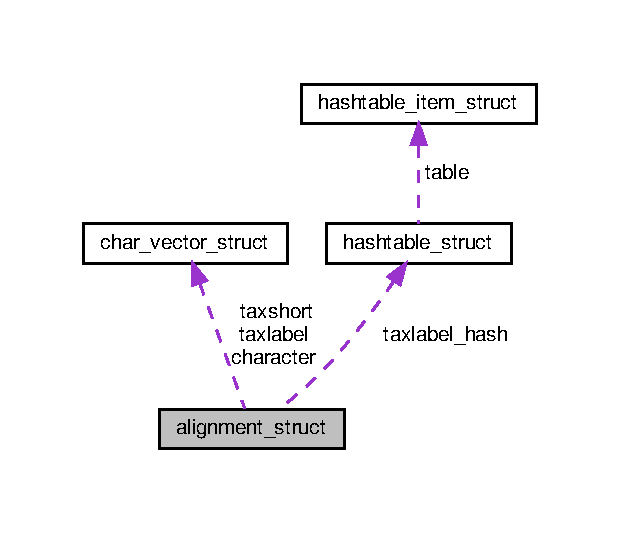
\includegraphics[width=298pt]{structalignment__struct__coll__graph}
\end{center}
\end{figure}
\subsubsection*{Data Fields}
\begin{DoxyCompactItemize}
\item 
\mbox{\Hypertarget{structalignment__struct_a90c549537ebcaeadf99cc214d9dbc8a6}\label{structalignment__struct_a90c549537ebcaeadf99cc214d9dbc8a6}} 
int {\bfseries ntax}
\item 
\mbox{\Hypertarget{structalignment__struct_a6586911ceefd68b40afb55f9c1f8cb37}\label{structalignment__struct_a6586911ceefd68b40afb55f9c1f8cb37}} 
int {\bfseries nchar}
\item 
\mbox{\Hypertarget{structalignment__struct_acae069aef1bf83529417d5503520dd20}\label{structalignment__struct_acae069aef1bf83529417d5503520dd20}} 
int {\bfseries npat}
\item 
\mbox{\Hypertarget{structalignment__struct_a5f298db9c22602b033f76d8e08469f0f}\label{structalignment__struct_a5f298db9c22602b033f76d8e08469f0f}} 
\hyperlink{structchar__vector__struct}{char\+\_\+vector} \hyperlink{structalignment__struct_a5f298db9c22602b033f76d8e08469f0f}{character}
\begin{DoxyCompactList}\small\item\em Number of species, sites and patterns according to sequence file. \end{DoxyCompactList}\item 
\mbox{\Hypertarget{structalignment__struct_ad0f1532a0b09d3987e99c51dd47b9415}\label{structalignment__struct_ad0f1532a0b09d3987e99c51dd47b9415}} 
\hyperlink{structchar__vector__struct}{char\+\_\+vector} \hyperlink{structalignment__struct_ad0f1532a0b09d3987e99c51dd47b9415}{taxlabel}
\begin{DoxyCompactList}\small\item\em Vector with aligned sequence for each taxon. \end{DoxyCompactList}\item 
\mbox{\Hypertarget{structalignment__struct_a193cea40877f33ff676015ed1d1cc876}\label{structalignment__struct_a193cea40877f33ff676015ed1d1cc876}} 
\hyperlink{structchar__vector__struct}{char\+\_\+vector} \hyperlink{structalignment__struct_a193cea40877f33ff676015ed1d1cc876}{taxshort}
\begin{DoxyCompactList}\small\item\em Taxon names from file. \end{DoxyCompactList}\item 
\mbox{\Hypertarget{structalignment__struct_ad0a2760951cbd2698aba10eb383ef942}\label{structalignment__struct_ad0a2760951cbd2698aba10eb383ef942}} 
\hyperlink{structhashtable__struct}{hashtable} \hyperlink{structalignment__struct_ad0a2760951cbd2698aba10eb383ef942}{taxlabel\+\_\+hash}
\begin{DoxyCompactList}\small\item\em Alias (short version) for taxon names that can be used in newick trees. \end{DoxyCompactList}\item 
\mbox{\Hypertarget{structalignment__struct_a18e5ad5b8fc356f20affd880be869405}\label{structalignment__struct_a18e5ad5b8fc356f20affd880be869405}} 
int \hyperlink{structalignment__struct_a18e5ad5b8fc356f20affd880be869405}{n\+\_\+charset}
\begin{DoxyCompactList}\small\item\em Lookup table with taxon names. \end{DoxyCompactList}\item 
\mbox{\Hypertarget{structalignment__struct_aabaec777f714bc9b052a667b95686fc0}\label{structalignment__struct_aabaec777f714bc9b052a667b95686fc0}} 
int $\ast$ \hyperlink{structalignment__struct_aabaec777f714bc9b052a667b95686fc0}{charset\+\_\+start}
\begin{DoxyCompactList}\small\item\em Number of gene segments (A\+S\+S\+U\+M\+P\+T\+I\+O\+NS B\+L\+O\+CK). \end{DoxyCompactList}\item 
\mbox{\Hypertarget{structalignment__struct_a667699e9b5ed61cec6fae87b0db11084}\label{structalignment__struct_a667699e9b5ed61cec6fae87b0db11084}} 
int $\ast$ {\bfseries charset\+\_\+end}
\item 
\mbox{\Hypertarget{structalignment__struct_a494093c32d2dcb61907f0e90c43fefd3}\label{structalignment__struct_a494093c32d2dcb61907f0e90c43fefd3}} 
\hyperlink{lowlevel_8h_a97a80ca1602ebf2303258971a2c938e2}{bool} \hyperlink{structalignment__struct_a494093c32d2dcb61907f0e90c43fefd3}{is\+\_\+aligned}
\begin{DoxyCompactList}\small\item\em Start and end of each gene segment (from 1...N\+C\+H\+AR) (A\+S\+S\+U\+M\+P\+T\+I\+O\+NS ). \end{DoxyCompactList}\item 
\mbox{\Hypertarget{structalignment__struct_ab599779f0254908bf21a78a503ee71bf}\label{structalignment__struct_ab599779f0254908bf21a78a503ee71bf}} 
int $\ast$ \hyperlink{structalignment__struct_ab599779f0254908bf21a78a503ee71bf}{site\+\_\+pattern}
\begin{DoxyCompactList}\small\item\em F\+A\+S\+TA files don\textquotesingle{}t need to be aligned; N\+E\+X\+US files do. \end{DoxyCompactList}\item 
\mbox{\Hypertarget{structalignment__struct_ac026c9e98a3ec37876fb6429b0e6fdb1}\label{structalignment__struct_ac026c9e98a3ec37876fb6429b0e6fdb1}} 
int $\ast$ \hyperlink{structalignment__struct_ac026c9e98a3ec37876fb6429b0e6fdb1}{pattern\+\_\+freq}
\begin{DoxyCompactList}\small\item\em pattern, in \hyperlink{structalignment__struct_a5f298db9c22602b033f76d8e08469f0f}{alignment\+\_\+struct\+::character}, to which original site belongs. \end{DoxyCompactList}\item 
\mbox{\Hypertarget{structalignment__struct_ac559cf9acf696eca7fea967c5c05dd18}\label{structalignment__struct_ac559cf9acf696eca7fea967c5c05dd18}} 
char $\ast$ \hyperlink{structalignment__struct_ac559cf9acf696eca7fea967c5c05dd18}{filename}
\begin{DoxyCompactList}\small\item\em if sequences are aligned, this is the frequency of each pattern. \end{DoxyCompactList}\item 
\mbox{\Hypertarget{structalignment__struct_a301172f590ef4fd3afb783cf417f6b1f}\label{structalignment__struct_a301172f590ef4fd3afb783cf417f6b1f}} 
int \hyperlink{structalignment__struct_a301172f590ef4fd3afb783cf417f6b1f}{ref\+\_\+counter}
\begin{DoxyCompactList}\small\item\em name of the original file, with extension removed \end{DoxyCompactList}\end{DoxyCompactItemize}


\subsubsection{Detailed Description}
Data from alignment file. 

The documentation for this struct was generated from the following file\+:\begin{DoxyCompactItemize}
\item 
\hyperlink{alignment_8h}{alignment.\+h}\end{DoxyCompactItemize}

\hypertarget{structarg__date}{}\subsection{arg\+\_\+date Struct Reference}
\label{structarg__date}\index{arg\+\_\+date@{arg\+\_\+date}}


Collaboration diagram for arg\+\_\+date\+:\nopagebreak
\begin{figure}[H]
\begin{center}
\leavevmode
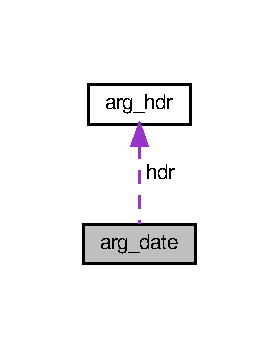
\includegraphics[width=134pt]{structarg__date__coll__graph}
\end{center}
\end{figure}
\subsubsection*{Data Fields}
\begin{DoxyCompactItemize}
\item 
\mbox{\Hypertarget{structarg__date_aaf2344a703e242481c22bdfe2a344463}\label{structarg__date_aaf2344a703e242481c22bdfe2a344463}} 
struct \hyperlink{structarg__hdr}{arg\+\_\+hdr} {\bfseries hdr}
\item 
\mbox{\Hypertarget{structarg__date_a6d4699868e7ac513e4c46d4009376a97}\label{structarg__date_a6d4699868e7ac513e4c46d4009376a97}} 
const char $\ast$ {\bfseries format}
\item 
\mbox{\Hypertarget{structarg__date_a50d9e3b29f556f30830bf07e4cc3bda1}\label{structarg__date_a50d9e3b29f556f30830bf07e4cc3bda1}} 
int {\bfseries count}
\item 
\mbox{\Hypertarget{structarg__date_a6d80a52ebb6691933f872fad22c281bc}\label{structarg__date_a6d80a52ebb6691933f872fad22c281bc}} 
struct tm $\ast$ {\bfseries tmval}
\end{DoxyCompactItemize}


The documentation for this struct was generated from the following file\+:\begin{DoxyCompactItemize}
\item 
argtable3.\+h\end{DoxyCompactItemize}

\hypertarget{structarg__dbl}{}\subsection{arg\+\_\+dbl Struct Reference}
\label{structarg__dbl}\index{arg\+\_\+dbl@{arg\+\_\+dbl}}


Collaboration diagram for arg\+\_\+dbl\+:\nopagebreak
\begin{figure}[H]
\begin{center}
\leavevmode
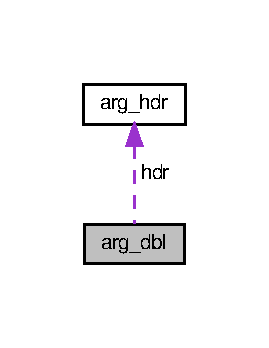
\includegraphics[width=129pt]{structarg__dbl__coll__graph}
\end{center}
\end{figure}
\subsubsection*{Data Fields}
\begin{DoxyCompactItemize}
\item 
\mbox{\Hypertarget{structarg__dbl_a0bf5455c02b70f1afc408597e81f8764}\label{structarg__dbl_a0bf5455c02b70f1afc408597e81f8764}} 
struct \hyperlink{structarg__hdr}{arg\+\_\+hdr} {\bfseries hdr}
\item 
\mbox{\Hypertarget{structarg__dbl_ab94e4d551bc7888e444dc1c7d040dfbb}\label{structarg__dbl_ab94e4d551bc7888e444dc1c7d040dfbb}} 
int {\bfseries count}
\item 
\mbox{\Hypertarget{structarg__dbl_ab928e87ab3a1ab5617b798fe02adfca1}\label{structarg__dbl_ab928e87ab3a1ab5617b798fe02adfca1}} 
double $\ast$ {\bfseries dval}
\end{DoxyCompactItemize}


The documentation for this struct was generated from the following file\+:\begin{DoxyCompactItemize}
\item 
argtable3.\+h\end{DoxyCompactItemize}

\hypertarget{structarg__end}{}\subsection{arg\+\_\+end Struct Reference}
\label{structarg__end}\index{arg\+\_\+end@{arg\+\_\+end}}


Collaboration diagram for arg\+\_\+end\+:\nopagebreak
\begin{figure}[H]
\begin{center}
\leavevmode
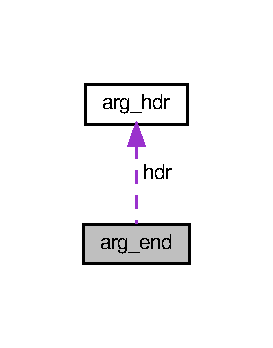
\includegraphics[width=131pt]{structarg__end__coll__graph}
\end{center}
\end{figure}
\subsubsection*{Data Fields}
\begin{DoxyCompactItemize}
\item 
\mbox{\Hypertarget{structarg__end_a5a09c1c05e96501d3c4807d7ffdeb7d0}\label{structarg__end_a5a09c1c05e96501d3c4807d7ffdeb7d0}} 
struct \hyperlink{structarg__hdr}{arg\+\_\+hdr} {\bfseries hdr}
\item 
\mbox{\Hypertarget{structarg__end_ae2996b25150e53ce4986c22f031492bd}\label{structarg__end_ae2996b25150e53ce4986c22f031492bd}} 
int {\bfseries count}
\item 
\mbox{\Hypertarget{structarg__end_a2ac6a156775d0c8a4570efea27270618}\label{structarg__end_a2ac6a156775d0c8a4570efea27270618}} 
int $\ast$ {\bfseries error}
\item 
\mbox{\Hypertarget{structarg__end_a147ab7eeebf5412bc47b6df87ec24b60}\label{structarg__end_a147ab7eeebf5412bc47b6df87ec24b60}} 
void $\ast$$\ast$ {\bfseries parent}
\item 
\mbox{\Hypertarget{structarg__end_abef36034ebc3ba28f53d1b6896e329a6}\label{structarg__end_abef36034ebc3ba28f53d1b6896e329a6}} 
const char $\ast$$\ast$ {\bfseries argval}
\end{DoxyCompactItemize}


The documentation for this struct was generated from the following file\+:\begin{DoxyCompactItemize}
\item 
argtable3.\+h\end{DoxyCompactItemize}

\hypertarget{structarg__file}{}\subsection{arg\+\_\+file Struct Reference}
\label{structarg__file}\index{arg\+\_\+file@{arg\+\_\+file}}


Collaboration diagram for arg\+\_\+file\+:\nopagebreak
\begin{figure}[H]
\begin{center}
\leavevmode
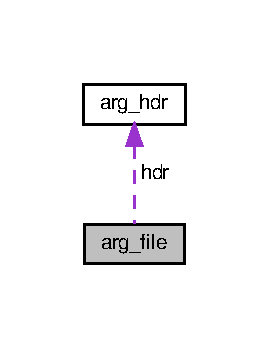
\includegraphics[width=129pt]{structarg__file__coll__graph}
\end{center}
\end{figure}
\subsubsection*{Data Fields}
\begin{DoxyCompactItemize}
\item 
\mbox{\Hypertarget{structarg__file_af4b8905c8b0417777376938221d4e42f}\label{structarg__file_af4b8905c8b0417777376938221d4e42f}} 
struct \hyperlink{structarg__hdr}{arg\+\_\+hdr} {\bfseries hdr}
\item 
\mbox{\Hypertarget{structarg__file_a5390027dbb693cbcc7630c96e5bdde83}\label{structarg__file_a5390027dbb693cbcc7630c96e5bdde83}} 
int {\bfseries count}
\item 
\mbox{\Hypertarget{structarg__file_a7822e37591de9d9a5ce78ed1f69b9bdc}\label{structarg__file_a7822e37591de9d9a5ce78ed1f69b9bdc}} 
const char $\ast$$\ast$ {\bfseries filename}
\item 
\mbox{\Hypertarget{structarg__file_a0765b5bbb8698b4e4c93b8613010568b}\label{structarg__file_a0765b5bbb8698b4e4c93b8613010568b}} 
const char $\ast$$\ast$ {\bfseries basename}
\item 
\mbox{\Hypertarget{structarg__file_a99aa017b9d7de188ad939653effae3e9}\label{structarg__file_a99aa017b9d7de188ad939653effae3e9}} 
const char $\ast$$\ast$ {\bfseries extension}
\end{DoxyCompactItemize}


The documentation for this struct was generated from the following file\+:\begin{DoxyCompactItemize}
\item 
argtable3.\+h\end{DoxyCompactItemize}

\hypertarget{structarg__hdr}{}\subsection{arg\+\_\+hdr Struct Reference}
\label{structarg__hdr}\index{arg\+\_\+hdr@{arg\+\_\+hdr}}
\subsubsection*{Data Fields}
\begin{DoxyCompactItemize}
\item 
\mbox{\Hypertarget{structarg__hdr_a9f3cb843aac57cfad9c1fe4de5cb14bd}\label{structarg__hdr_a9f3cb843aac57cfad9c1fe4de5cb14bd}} 
char {\bfseries flag}
\item 
\mbox{\Hypertarget{structarg__hdr_a48c0d7fb876e6f6e57850f282373ec0e}\label{structarg__hdr_a48c0d7fb876e6f6e57850f282373ec0e}} 
const char $\ast$ {\bfseries shortopts}
\item 
\mbox{\Hypertarget{structarg__hdr_a10c111dc87cba922999fb3df9e0fddb9}\label{structarg__hdr_a10c111dc87cba922999fb3df9e0fddb9}} 
const char $\ast$ {\bfseries longopts}
\item 
\mbox{\Hypertarget{structarg__hdr_ab2ce9d2572f8da0d48be98d6c2cbddf3}\label{structarg__hdr_ab2ce9d2572f8da0d48be98d6c2cbddf3}} 
const char $\ast$ {\bfseries datatype}
\item 
\mbox{\Hypertarget{structarg__hdr_a1d4fe07468a704f059f38e8e144dc5ac}\label{structarg__hdr_a1d4fe07468a704f059f38e8e144dc5ac}} 
const char $\ast$ {\bfseries glossary}
\item 
\mbox{\Hypertarget{structarg__hdr_a6dd2a2f1a4394a68abf64b11d80c5c64}\label{structarg__hdr_a6dd2a2f1a4394a68abf64b11d80c5c64}} 
int {\bfseries mincount}
\item 
\mbox{\Hypertarget{structarg__hdr_a7eb5f9be879e4214cd3fe42bac8ce99f}\label{structarg__hdr_a7eb5f9be879e4214cd3fe42bac8ce99f}} 
int {\bfseries maxcount}
\item 
\mbox{\Hypertarget{structarg__hdr_a4720cbc498bd74a55612edc054f8d670}\label{structarg__hdr_a4720cbc498bd74a55612edc054f8d670}} 
void $\ast$ {\bfseries parent}
\item 
\mbox{\Hypertarget{structarg__hdr_a6ed05b7c388dea710b41c8da72bfe987}\label{structarg__hdr_a6ed05b7c388dea710b41c8da72bfe987}} 
arg\+\_\+resetfn $\ast$ {\bfseries resetfn}
\item 
\mbox{\Hypertarget{structarg__hdr_a263be45e6d91e91fea4fc539df9a54fd}\label{structarg__hdr_a263be45e6d91e91fea4fc539df9a54fd}} 
arg\+\_\+scanfn $\ast$ {\bfseries scanfn}
\item 
\mbox{\Hypertarget{structarg__hdr_ae7435d6a03fb8a32fd6fa64fbd707845}\label{structarg__hdr_ae7435d6a03fb8a32fd6fa64fbd707845}} 
arg\+\_\+checkfn $\ast$ {\bfseries checkfn}
\item 
\mbox{\Hypertarget{structarg__hdr_a38d5e3d139e6cdb04474aede48439a2f}\label{structarg__hdr_a38d5e3d139e6cdb04474aede48439a2f}} 
arg\+\_\+errorfn $\ast$ {\bfseries errorfn}
\item 
\mbox{\Hypertarget{structarg__hdr_ac4be91967af1c23425c4a70383d5f2d6}\label{structarg__hdr_ac4be91967af1c23425c4a70383d5f2d6}} 
void $\ast$ {\bfseries priv}
\end{DoxyCompactItemize}


The documentation for this struct was generated from the following file\+:\begin{DoxyCompactItemize}
\item 
argtable3.\+h\end{DoxyCompactItemize}

\hypertarget{structarg__int}{}\subsection{arg\+\_\+int Struct Reference}
\label{structarg__int}\index{arg\+\_\+int@{arg\+\_\+int}}


Collaboration diagram for arg\+\_\+int\+:\nopagebreak
\begin{figure}[H]
\begin{center}
\leavevmode
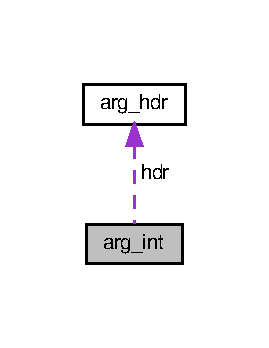
\includegraphics[width=129pt]{structarg__int__coll__graph}
\end{center}
\end{figure}
\subsubsection*{Data Fields}
\begin{DoxyCompactItemize}
\item 
\mbox{\Hypertarget{structarg__int_a2d761e688517421de2b5c6a7b7a4e164}\label{structarg__int_a2d761e688517421de2b5c6a7b7a4e164}} 
struct \hyperlink{structarg__hdr}{arg\+\_\+hdr} {\bfseries hdr}
\item 
\mbox{\Hypertarget{structarg__int_ac27c689313154ed186702d101c8157db}\label{structarg__int_ac27c689313154ed186702d101c8157db}} 
int {\bfseries count}
\item 
\mbox{\Hypertarget{structarg__int_ae552c7d918197309d6ee227dbfb8ed2e}\label{structarg__int_ae552c7d918197309d6ee227dbfb8ed2e}} 
int $\ast$ {\bfseries ival}
\end{DoxyCompactItemize}


The documentation for this struct was generated from the following file\+:\begin{DoxyCompactItemize}
\item 
argtable3.\+h\end{DoxyCompactItemize}

\hypertarget{structarg__lit}{}\subsection{arg\+\_\+lit Struct Reference}
\label{structarg__lit}\index{arg\+\_\+lit@{arg\+\_\+lit}}


Collaboration diagram for arg\+\_\+lit\+:\nopagebreak
\begin{figure}[H]
\begin{center}
\leavevmode
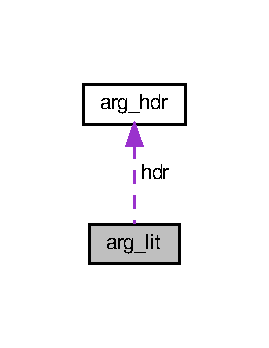
\includegraphics[width=129pt]{structarg__lit__coll__graph}
\end{center}
\end{figure}
\subsubsection*{Data Fields}
\begin{DoxyCompactItemize}
\item 
\mbox{\Hypertarget{structarg__lit_ab01efa22bd97c4e4dd1f00a2626e85e9}\label{structarg__lit_ab01efa22bd97c4e4dd1f00a2626e85e9}} 
struct \hyperlink{structarg__hdr}{arg\+\_\+hdr} {\bfseries hdr}
\item 
\mbox{\Hypertarget{structarg__lit_ab60f65d2cba968ee42e089047a39cf1c}\label{structarg__lit_ab60f65d2cba968ee42e089047a39cf1c}} 
int {\bfseries count}
\end{DoxyCompactItemize}


The documentation for this struct was generated from the following file\+:\begin{DoxyCompactItemize}
\item 
argtable3.\+h\end{DoxyCompactItemize}

\hypertarget{structarg__rem}{}\subsection{arg\+\_\+rem Struct Reference}
\label{structarg__rem}\index{arg\+\_\+rem@{arg\+\_\+rem}}


Collaboration diagram for arg\+\_\+rem\+:\nopagebreak
\begin{figure}[H]
\begin{center}
\leavevmode
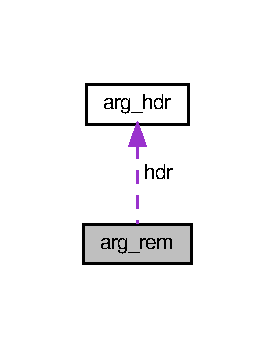
\includegraphics[width=132pt]{structarg__rem__coll__graph}
\end{center}
\end{figure}
\subsubsection*{Data Fields}
\begin{DoxyCompactItemize}
\item 
\mbox{\Hypertarget{structarg__rem_afc389187361d2c1f2b18760b59dc7bfc}\label{structarg__rem_afc389187361d2c1f2b18760b59dc7bfc}} 
struct \hyperlink{structarg__hdr}{arg\+\_\+hdr} {\bfseries hdr}
\end{DoxyCompactItemize}


The documentation for this struct was generated from the following file\+:\begin{DoxyCompactItemize}
\item 
argtable3.\+h\end{DoxyCompactItemize}

\hypertarget{structarg__rex}{}\subsection{arg\+\_\+rex Struct Reference}
\label{structarg__rex}\index{arg\+\_\+rex@{arg\+\_\+rex}}


Collaboration diagram for arg\+\_\+rex\+:\nopagebreak
\begin{figure}[H]
\begin{center}
\leavevmode
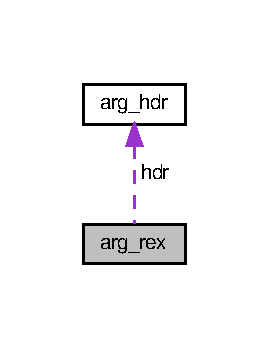
\includegraphics[width=129pt]{structarg__rex__coll__graph}
\end{center}
\end{figure}
\subsubsection*{Data Fields}
\begin{DoxyCompactItemize}
\item 
\mbox{\Hypertarget{structarg__rex_af009bf62545082e4d9128f86846bc320}\label{structarg__rex_af009bf62545082e4d9128f86846bc320}} 
struct \hyperlink{structarg__hdr}{arg\+\_\+hdr} {\bfseries hdr}
\item 
\mbox{\Hypertarget{structarg__rex_aaf9bd8bfb7d71e067c33dcaaa172fcad}\label{structarg__rex_aaf9bd8bfb7d71e067c33dcaaa172fcad}} 
int {\bfseries count}
\item 
\mbox{\Hypertarget{structarg__rex_a3508cb79a9ff78ac5d074b6fc8a34b31}\label{structarg__rex_a3508cb79a9ff78ac5d074b6fc8a34b31}} 
const char $\ast$$\ast$ {\bfseries sval}
\end{DoxyCompactItemize}


The documentation for this struct was generated from the following file\+:\begin{DoxyCompactItemize}
\item 
argtable3.\+h\end{DoxyCompactItemize}

\hypertarget{structarg__str}{}\subsection{arg\+\_\+str Struct Reference}
\label{structarg__str}\index{arg\+\_\+str@{arg\+\_\+str}}


Collaboration diagram for arg\+\_\+str\+:\nopagebreak
\begin{figure}[H]
\begin{center}
\leavevmode
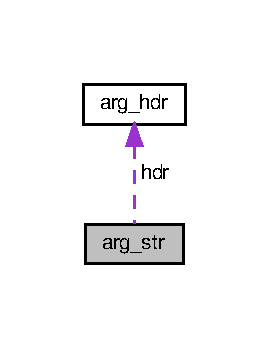
\includegraphics[width=129pt]{structarg__str__coll__graph}
\end{center}
\end{figure}
\subsubsection*{Data Fields}
\begin{DoxyCompactItemize}
\item 
\mbox{\Hypertarget{structarg__str_ac4547101ac4ec560e101979423be8289}\label{structarg__str_ac4547101ac4ec560e101979423be8289}} 
struct \hyperlink{structarg__hdr}{arg\+\_\+hdr} {\bfseries hdr}
\item 
\mbox{\Hypertarget{structarg__str_aaa99fd17e707232cb78e96fafb003d4f}\label{structarg__str_aaa99fd17e707232cb78e96fafb003d4f}} 
int {\bfseries count}
\item 
\mbox{\Hypertarget{structarg__str_ad41813dbbf8d8666a45bf071437ca61d}\label{structarg__str_ad41813dbbf8d8666a45bf071437ca61d}} 
const char $\ast$$\ast$ {\bfseries sval}
\end{DoxyCompactItemize}


The documentation for this struct was generated from the following file\+:\begin{DoxyCompactItemize}
\item 
argtable3.\+h\end{DoxyCompactItemize}

\hypertarget{structbinary__parsimony__datamatrix__struct}{}\subsection{binary\+\_\+parsimony\+\_\+datamatrix\+\_\+struct Struct Reference}
\label{structbinary__parsimony__datamatrix__struct}\index{binary\+\_\+parsimony\+\_\+datamatrix\+\_\+struct@{binary\+\_\+parsimony\+\_\+datamatrix\+\_\+struct}}


used by matrix representation with parsimony (01 10 11 sequences)  




{\ttfamily \#include $<$parsimony.\+h$>$}

\subsubsection*{Data Fields}
\begin{DoxyCompactItemize}
\item 
\mbox{\Hypertarget{structbinary__parsimony__datamatrix__struct_a424911f4f74135af958f97f25ceaf4ad}\label{structbinary__parsimony__datamatrix__struct_a424911f4f74135af958f97f25ceaf4ad}} 
int {\bfseries ntax}
\item 
\mbox{\Hypertarget{structbinary__parsimony__datamatrix__struct_ad2e17453dc6a1835683753232d5b9412}\label{structbinary__parsimony__datamatrix__struct_ad2e17453dc6a1835683753232d5b9412}} 
int {\bfseries nchar}
\item 
\mbox{\Hypertarget{structbinary__parsimony__datamatrix__struct_a673bd1a74e442138332c4c8321f54949}\label{structbinary__parsimony__datamatrix__struct_a673bd1a74e442138332c4c8321f54949}} 
int \hyperlink{structbinary__parsimony__datamatrix__struct_a673bd1a74e442138332c4c8321f54949}{i}
\begin{DoxyCompactList}\small\item\em number of taxa, distinct sites (patterns), and index to current (last) column \end{DoxyCompactList}\item 
\mbox{\Hypertarget{structbinary__parsimony__datamatrix__struct_a137caa1e489a54f80fa6e517b6f9626d}\label{structbinary__parsimony__datamatrix__struct_a137caa1e489a54f80fa6e517b6f9626d}} 
\hyperlink{lowlevel_8h_a97a80ca1602ebf2303258971a2c938e2}{bool} $\ast$$\ast$ \hyperlink{structbinary__parsimony__datamatrix__struct_a137caa1e489a54f80fa6e517b6f9626d}{s}
\begin{DoxyCompactList}\small\item\em 1 (01) and 2 (10) are the two binary states, with 3 (11) being undetermined \end{DoxyCompactList}\item 
\mbox{\Hypertarget{structbinary__parsimony__datamatrix__struct_a246a8e030ece949dc7a0c48946900258}\label{structbinary__parsimony__datamatrix__struct_a246a8e030ece949dc7a0c48946900258}} 
int $\ast$ {\bfseries freq}
\item 
\mbox{\Hypertarget{structbinary__parsimony__datamatrix__struct_ac58346b932eae6dc2cc2ee8857076073}\label{structbinary__parsimony__datamatrix__struct_ac58346b932eae6dc2cc2ee8857076073}} 
int \hyperlink{structbinary__parsimony__datamatrix__struct_ac58346b932eae6dc2cc2ee8857076073}{freq\+\_\+sum}
\begin{DoxyCompactList}\small\item\em frequency of pattern. \end{DoxyCompactList}\item 
\mbox{\Hypertarget{structbinary__parsimony__datamatrix__struct_afb10c6a469cbf1acca33c37e234aa708}\label{structbinary__parsimony__datamatrix__struct_afb10c6a469cbf1acca33c37e234aa708}} 
int $\ast$ \hyperlink{structbinary__parsimony__datamatrix__struct_afb10c6a469cbf1acca33c37e234aa708}{occupancy}
\begin{DoxyCompactList}\small\item\em how many species represented by each bipartition \end{DoxyCompactList}\item 
\mbox{\Hypertarget{structbinary__parsimony__datamatrix__struct_a4acbe9e6568767e51cabd060541f24e6}\label{structbinary__parsimony__datamatrix__struct_a4acbe9e6568767e51cabd060541f24e6}} 
uint32\+\_\+t $\ast$ \hyperlink{structbinary__parsimony__datamatrix__struct_a4acbe9e6568767e51cabd060541f24e6}{col\+\_\+hash}
\begin{DoxyCompactList}\small\item\em hash value of each column, to speed up comparisons \end{DoxyCompactList}\item 
\mbox{\Hypertarget{structbinary__parsimony__datamatrix__struct_a2064ac0302bcbe428c83c5768fa266a7}\label{structbinary__parsimony__datamatrix__struct_a2064ac0302bcbe428c83c5768fa266a7}} 
int \hyperlink{structbinary__parsimony__datamatrix__struct_a2064ac0302bcbe428c83c5768fa266a7}{ref\+\_\+counter}
\begin{DoxyCompactList}\small\item\em how many places have a pointer to this instance \end{DoxyCompactList}\end{DoxyCompactItemize}


\subsubsection{Detailed Description}
used by matrix representation with parsimony (01 10 11 sequences) 

The documentation for this struct was generated from the following file\+:\begin{DoxyCompactItemize}
\item 
\hyperlink{parsimony_8h}{parsimony.\+h}\end{DoxyCompactItemize}

\hypertarget{structbinary__parsimony__struct}{}\subsection{binary\+\_\+parsimony\+\_\+struct Struct Reference}
\label{structbinary__parsimony__struct}\index{binary\+\_\+parsimony\+\_\+struct@{binary\+\_\+parsimony\+\_\+struct}}


Collaboration diagram for binary\+\_\+parsimony\+\_\+struct\+:\nopagebreak
\begin{figure}[H]
\begin{center}
\leavevmode
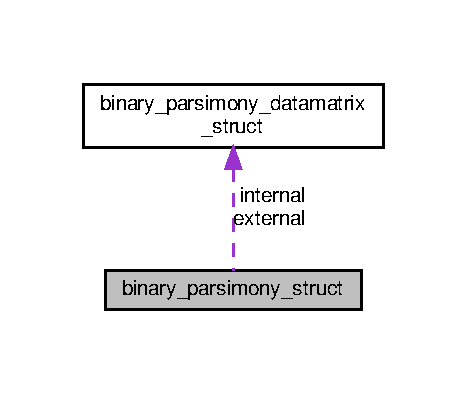
\includegraphics[width=224pt]{structbinary__parsimony__struct__coll__graph}
\end{center}
\end{figure}
\subsubsection*{Data Fields}
\begin{DoxyCompactItemize}
\item 
\mbox{\Hypertarget{structbinary__parsimony__struct_a8002f973d4c738ceb44ff459833965b2}\label{structbinary__parsimony__struct_a8002f973d4c738ceb44ff459833965b2}} 
int $\ast$ \hyperlink{structbinary__parsimony__struct_a8002f973d4c738ceb44ff459833965b2}{score}
\begin{DoxyCompactList}\small\item\em parsimony score per pattern \end{DoxyCompactList}\item 
\mbox{\Hypertarget{structbinary__parsimony__struct_a7ee8780b9cbca6b4b5a6415ef0a47377}\label{structbinary__parsimony__struct_a7ee8780b9cbca6b4b5a6415ef0a47377}} 
\hyperlink{structbinary__parsimony__datamatrix__struct}{binary\+\_\+parsimony\+\_\+datamatrix} {\bfseries external}
\item 
\mbox{\Hypertarget{structbinary__parsimony__struct_a27c3b203843a26338af931010c7666de}\label{structbinary__parsimony__struct_a27c3b203843a26338af931010c7666de}} 
\hyperlink{structbinary__parsimony__datamatrix__struct}{binary\+\_\+parsimony\+\_\+datamatrix} \hyperlink{structbinary__parsimony__struct_a27c3b203843a26338af931010c7666de}{internal}
\begin{DoxyCompactList}\small\item\em binary matrices for leaves and for internal nodes \end{DoxyCompactList}\item 
\mbox{\Hypertarget{structbinary__parsimony__struct_a6515933c8e71aba6cb2795d9ecfd78b8}\label{structbinary__parsimony__struct_a6515933c8e71aba6cb2795d9ecfd78b8}} 
double {\bfseries costs} \mbox{[}4\mbox{]}
\item 
\mbox{\Hypertarget{structbinary__parsimony__struct_a5aab1b8c99ac264cba1c17612f72edea}\label{structbinary__parsimony__struct_a5aab1b8c99ac264cba1c17612f72edea}} 
int \hyperlink{structbinary__parsimony__struct_a5aab1b8c99ac264cba1c17612f72edea}{ref\+\_\+counter}
\begin{DoxyCompactList}\small\item\em how many places have a pointer to this instance \end{DoxyCompactList}\end{DoxyCompactItemize}


The documentation for this struct was generated from the following file\+:\begin{DoxyCompactItemize}
\item 
\hyperlink{parsimony_8h}{parsimony.\+h}\end{DoxyCompactItemize}

\hypertarget{structbiomcmc__rng__struct}{}\subsection{biomcmc\+\_\+rng\+\_\+struct Struct Reference}
\label{structbiomcmc__rng__struct}\index{biomcmc\+\_\+rng\+\_\+struct@{biomcmc\+\_\+rng\+\_\+struct}}


Random number structure (combined Tausworthe algorithm)  




{\ttfamily \#include $<$random\+\_\+number.\+h$>$}



Collaboration diagram for biomcmc\+\_\+rng\+\_\+struct\+:\nopagebreak
\begin{figure}[H]
\begin{center}
\leavevmode
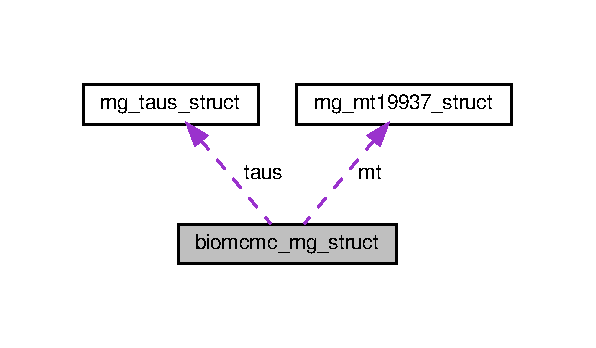
\includegraphics[width=286pt]{structbiomcmc__rng__struct__coll__graph}
\end{center}
\end{figure}
\subsubsection*{Data Fields}
\begin{DoxyCompactItemize}
\item 
\mbox{\Hypertarget{structbiomcmc__rng__struct_a8d4d5fdf7a1c52aabb06b39446c3ed93}\label{structbiomcmc__rng__struct_a8d4d5fdf7a1c52aabb06b39446c3ed93}} 
\hyperlink{structrng__taus__struct}{rng\+\_\+taus\+\_\+struct} {\bfseries taus}
\item 
\mbox{\Hypertarget{structbiomcmc__rng__struct_a0d35534d56f6c0b57d76495319e8f219}\label{structbiomcmc__rng__struct_a0d35534d56f6c0b57d76495319e8f219}} 
\hyperlink{structrng__mt19937__struct}{rng\+\_\+mt19937\+\_\+struct} \hyperlink{structbiomcmc__rng__struct_a0d35534d56f6c0b57d76495319e8f219}{mt}
\begin{DoxyCompactList}\small\item\em Tausworthe linear feedback shift-\/register from G\+SL. \end{DoxyCompactList}\item 
\mbox{\Hypertarget{structbiomcmc__rng__struct_ae26faaf87d679a2b9236ba303471cee2}\label{structbiomcmc__rng__struct_ae26faaf87d679a2b9236ba303471cee2}} 
uint64\+\_\+t \hyperlink{structbiomcmc__rng__struct_ae26faaf87d679a2b9236ba303471cee2}{bit32}
\begin{DoxyCompactList}\small\item\em 64 bits Mersenne Twister from Matsumoto\textquotesingle{}s webpage \end{DoxyCompactList}\item 
\mbox{\Hypertarget{structbiomcmc__rng__struct_ae0279edd5e5e20a4784ef67a6e57a638}\label{structbiomcmc__rng__struct_ae0279edd5e5e20a4784ef67a6e57a638}} 
\hyperlink{lowlevel_8h_a97a80ca1602ebf2303258971a2c938e2}{bool} \hyperlink{structbiomcmc__rng__struct_ae0279edd5e5e20a4784ef67a6e57a638}{have\+\_\+bit32}
\begin{DoxyCompactList}\small\item\em temporary values when only 32 bits are necessary \end{DoxyCompactList}\item 
\mbox{\Hypertarget{structbiomcmc__rng__struct_a387dd92d4bb3218530d7187fdb23a113}\label{structbiomcmc__rng__struct_a387dd92d4bb3218530d7187fdb23a113}} 
double \hyperlink{structbiomcmc__rng__struct_a387dd92d4bb3218530d7187fdb23a113}{rnorm32}
\begin{DoxyCompactList}\small\item\em when using 32 bits we first check if we have one stored \end{DoxyCompactList}\item 
\mbox{\Hypertarget{structbiomcmc__rng__struct_a7e321a23ca5d7305a54374bf98358148}\label{structbiomcmc__rng__struct_a7e321a23ca5d7305a54374bf98358148}} 
double {\bfseries rnorm64}
\item 
\mbox{\Hypertarget{structbiomcmc__rng__struct_a2d50ad99ab3615eb6ada4f176dc00f7d}\label{structbiomcmc__rng__struct_a2d50ad99ab3615eb6ada4f176dc00f7d}} 
\hyperlink{lowlevel_8h_a97a80ca1602ebf2303258971a2c938e2}{bool} \hyperlink{structbiomcmc__rng__struct_a2d50ad99ab3615eb6ada4f176dc00f7d}{have\+\_\+rnorm32}
\begin{DoxyCompactList}\small\item\em stored standard normal random values with 32 and 52 bits of precision \end{DoxyCompactList}\item 
\mbox{\Hypertarget{structbiomcmc__rng__struct_ad38ad14ad51ed51b49315cc944dc9bee}\label{structbiomcmc__rng__struct_ad38ad14ad51ed51b49315cc944dc9bee}} 
\hyperlink{lowlevel_8h_a97a80ca1602ebf2303258971a2c938e2}{bool} {\bfseries have\+\_\+rnorm64}
\end{DoxyCompactItemize}


\subsubsection{Detailed Description}
Random number structure (combined Tausworthe algorithm) 

The documentation for this struct was generated from the following file\+:\begin{DoxyCompactItemize}
\item 
\hyperlink{random__number_8h}{random\+\_\+number.\+h}\end{DoxyCompactItemize}

\hypertarget{structbip__hashitem__struct}{}\subsection{bip\+\_\+hashitem\+\_\+struct Struct Reference}
\label{structbip__hashitem__struct}\index{bip\+\_\+hashitem\+\_\+struct@{bip\+\_\+hashitem\+\_\+struct}}


key (bipartition) and value (frequency) pair for hash table of bipartitions  




{\ttfamily \#include $<$hashtable.\+h$>$}



Collaboration diagram for bip\+\_\+hashitem\+\_\+struct\+:\nopagebreak
\begin{figure}[H]
\begin{center}
\leavevmode
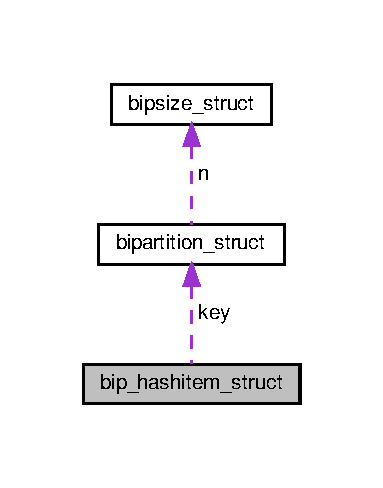
\includegraphics[width=184pt]{structbip__hashitem__struct__coll__graph}
\end{center}
\end{figure}
\subsubsection*{Data Fields}
\begin{DoxyCompactItemize}
\item 
\mbox{\Hypertarget{structbip__hashitem__struct_a12ef81b65e6d8b0e3d09cf75dc45b9d5}\label{structbip__hashitem__struct_a12ef81b65e6d8b0e3d09cf75dc45b9d5}} 
\hyperlink{structbipartition__struct}{bipartition} {\bfseries key}
\item 
\mbox{\Hypertarget{structbip__hashitem__struct_a72dfaa13a770d59596036a35c46cddc2}\label{structbip__hashitem__struct_a72dfaa13a770d59596036a35c46cddc2}} 
int \hyperlink{structbip__hashitem__struct_a72dfaa13a770d59596036a35c46cddc2}{count}
\begin{DoxyCompactList}\small\item\em pointer to bipartition (must update ref\+\_\+counter) \end{DoxyCompactList}\end{DoxyCompactItemize}


\subsubsection{Detailed Description}
key (bipartition) and value (frequency) pair for hash table of bipartitions 

The documentation for this struct was generated from the following file\+:\begin{DoxyCompactItemize}
\item 
\hyperlink{hashtable_8h}{hashtable.\+h}\end{DoxyCompactItemize}

\hypertarget{structbip__hashtable__struct}{}\subsection{bip\+\_\+hashtable\+\_\+struct Struct Reference}
\label{structbip__hashtable__struct}\index{bip\+\_\+hashtable\+\_\+struct@{bip\+\_\+hashtable\+\_\+struct}}


Hash table of bipartitions (see \hyperlink{structhashtable__struct_ae77d63df7a927e68de61d431d5bc0ddc}{hashtable.\+h} for original version, with string keys and integer values)  




{\ttfamily \#include $<$hashtable.\+h$>$}



Collaboration diagram for bip\+\_\+hashtable\+\_\+struct\+:\nopagebreak
\begin{figure}[H]
\begin{center}
\leavevmode
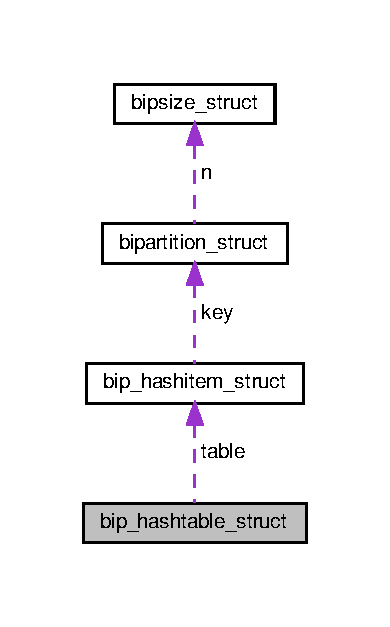
\includegraphics[width=187pt]{structbip__hashtable__struct__coll__graph}
\end{center}
\end{figure}
\subsubsection*{Data Fields}
\begin{DoxyCompactItemize}
\item 
\mbox{\Hypertarget{structbip__hashtable__struct_a12c1565ff6c6070f7d478bf8aa944432}\label{structbip__hashtable__struct_a12c1565ff6c6070f7d478bf8aa944432}} 
int {\bfseries size}
\item 
\mbox{\Hypertarget{structbip__hashtable__struct_a25e9a1bf231580249c88a75e6b714c15}\label{structbip__hashtable__struct_a25e9a1bf231580249c88a75e6b714c15}} 
int \hyperlink{structbip__hashtable__struct_a25e9a1bf231580249c88a75e6b714c15}{probelength}
\begin{DoxyCompactList}\small\item\em Table size. \end{DoxyCompactList}\item 
\mbox{\Hypertarget{structbip__hashtable__struct_abb13b3f66308184429bca8b7f4a5f67f}\label{structbip__hashtable__struct_abb13b3f66308184429bca8b7f4a5f67f}} 
int \hyperlink{structbip__hashtable__struct_abb13b3f66308184429bca8b7f4a5f67f}{maxfreq}
\begin{DoxyCompactList}\small\item\em Number of collisions before empty slot is found. \end{DoxyCompactList}\item 
\mbox{\Hypertarget{structbip__hashtable__struct_a25524e54647fc07fef816a68b253d18f}\label{structbip__hashtable__struct_a25524e54647fc07fef816a68b253d18f}} 
uint32\+\_\+t \hyperlink{structbip__hashtable__struct_a25524e54647fc07fef816a68b253d18f}{h}
\begin{DoxyCompactList}\small\item\em frequency (integer) of most frequent bipartition \end{DoxyCompactList}\item 
\mbox{\Hypertarget{structbip__hashtable__struct_a0ff51403063e40a6c0e50c011450eaef}\label{structbip__hashtable__struct_a0ff51403063e40a6c0e50c011450eaef}} 
uint32\+\_\+t \hyperlink{structbip__hashtable__struct_a0ff51403063e40a6c0e50c011450eaef}{a1}
\begin{DoxyCompactList}\small\item\em Value set by hash(). Used in hash1() and hash2() to avoid calling hash() again. \end{DoxyCompactList}\item 
\mbox{\Hypertarget{structbip__hashtable__struct_a6f7552b78ecdf55700939433b37e87e6}\label{structbip__hashtable__struct_a6f7552b78ecdf55700939433b37e87e6}} 
uint32\+\_\+t {\bfseries a2}
\item 
\mbox{\Hypertarget{structbip__hashtable__struct_a168857c41fa3b69ed7e182b54d6c0eec}\label{structbip__hashtable__struct_a168857c41fa3b69ed7e182b54d6c0eec}} 
uint32\+\_\+t {\bfseries b1}
\item 
\mbox{\Hypertarget{structbip__hashtable__struct_a1a121d5300cd180192ff50d2e5d07e73}\label{structbip__hashtable__struct_a1a121d5300cd180192ff50d2e5d07e73}} 
uint32\+\_\+t {\bfseries b2}
\item 
\mbox{\Hypertarget{structbip__hashtable__struct_a069f02825833c148d16c419b1e8e6df2}\label{structbip__hashtable__struct_a069f02825833c148d16c419b1e8e6df2}} 
uint32\+\_\+t \hyperlink{structbip__hashtable__struct_a069f02825833c148d16c419b1e8e6df2}{P}
\begin{DoxyCompactList}\small\item\em Random values used in hash functions. \end{DoxyCompactList}\item 
\mbox{\Hypertarget{structbip__hashtable__struct_aac0467a670a14218bc714cacbbda208a}\label{structbip__hashtable__struct_aac0467a670a14218bc714cacbbda208a}} 
\hyperlink{structbip__hashitem__struct}{bip\+\_\+hashitem} $\ast$ {\bfseries table}
\item 
\mbox{\Hypertarget{structbip__hashtable__struct_a5dea92a2e0bb95a46baf5fe77822d479}\label{structbip__hashtable__struct_a5dea92a2e0bb95a46baf5fe77822d479}} 
int \hyperlink{structbip__hashtable__struct_a5dea92a2e0bb95a46baf5fe77822d479}{ref\+\_\+counter}
\begin{DoxyCompactList}\small\item\em Vector with key/value pairs. \end{DoxyCompactList}\end{DoxyCompactItemize}


\subsubsection{Detailed Description}
Hash table of bipartitions (see \hyperlink{structhashtable__struct_ae77d63df7a927e68de61d431d5bc0ddc}{hashtable.\+h} for original version, with string keys and integer values) 

The documentation for this struct was generated from the following file\+:\begin{DoxyCompactItemize}
\item 
\hyperlink{hashtable_8h}{hashtable.\+h}\end{DoxyCompactItemize}

\hypertarget{structbipartition__struct}{}\subsection{bipartition\+\_\+struct Struct Reference}
\label{structbipartition__struct}\index{bipartition\+\_\+struct@{bipartition\+\_\+struct}}


Bit-\/string representation of splits.  




{\ttfamily \#include $<$bipartition.\+h$>$}



Collaboration diagram for bipartition\+\_\+struct\+:\nopagebreak
\begin{figure}[H]
\begin{center}
\leavevmode
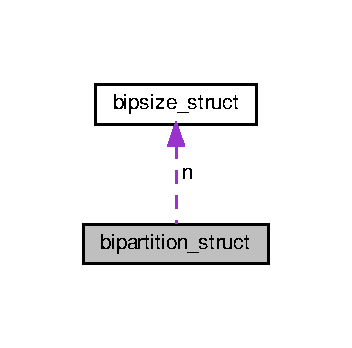
\includegraphics[width=169pt]{structbipartition__struct__coll__graph}
\end{center}
\end{figure}
\subsubsection*{Data Fields}
\begin{DoxyCompactItemize}
\item 
\mbox{\Hypertarget{structbipartition__struct_a2cb01205ff03325f27f67237ec4945a2}\label{structbipartition__struct_a2cb01205ff03325f27f67237ec4945a2}} 
uint64\+\_\+t $\ast$ \hyperlink{structbipartition__struct_a2cb01205ff03325f27f67237ec4945a2}{bs}
\begin{DoxyCompactList}\small\item\em Representation of a bipartition by a vector of integers (bitstrings). \end{DoxyCompactList}\item 
\mbox{\Hypertarget{structbipartition__struct_a9ab91a7d30c2e9b39f379886be39f949}\label{structbipartition__struct_a9ab91a7d30c2e9b39f379886be39f949}} 
int \hyperlink{structbipartition__struct_a9ab91a7d30c2e9b39f379886be39f949}{n\+\_\+ones}
\begin{DoxyCompactList}\small\item\em Counter (number of \char`\"{}one\char`\"{}s) \end{DoxyCompactList}\item 
\mbox{\Hypertarget{structbipartition__struct_a55bed1bfc645016d5f4e67fc3a5d1915}\label{structbipartition__struct_a55bed1bfc645016d5f4e67fc3a5d1915}} 
\hyperlink{structbipsize__struct}{bipsize} \hyperlink{structbipartition__struct_a55bed1bfc645016d5f4e67fc3a5d1915}{n}
\begin{DoxyCompactList}\small\item\em number of bits (leaves), vector size and mask \end{DoxyCompactList}\item 
\mbox{\Hypertarget{structbipartition__struct_aa6638f51d788a4b0475318be05a82a7b}\label{structbipartition__struct_aa6638f51d788a4b0475318be05a82a7b}} 
int \hyperlink{structbipartition__struct_aa6638f51d788a4b0475318be05a82a7b}{ref\+\_\+counter}
\begin{DoxyCompactList}\small\item\em How many times this struct is being referenced. \end{DoxyCompactList}\end{DoxyCompactItemize}


\subsubsection{Detailed Description}
Bit-\/string representation of splits. 

The documentation for this struct was generated from the following file\+:\begin{DoxyCompactItemize}
\item 
\hyperlink{bipartition_8h}{bipartition.\+h}\end{DoxyCompactItemize}

\hypertarget{structbipsize__struct}{}\subsection{bipsize\+\_\+struct Struct Reference}
\label{structbipsize__struct}\index{bipsize\+\_\+struct@{bipsize\+\_\+struct}}
\subsubsection*{Data Fields}
\begin{DoxyCompactItemize}
\item 
\mbox{\Hypertarget{structbipsize__struct_aaa074f83194be279e68e0d75ed600661}\label{structbipsize__struct_aaa074f83194be279e68e0d75ed600661}} 
uint64\+\_\+t \hyperlink{structbipsize__struct_aaa074f83194be279e68e0d75ed600661}{mask}
\begin{DoxyCompactList}\small\item\em mask to make sure we consider only active positions (of last bitstring) \end{DoxyCompactList}\item 
\mbox{\Hypertarget{structbipsize__struct_a6e10e8346b588d6f067390563555c715}\label{structbipsize__struct_a6e10e8346b588d6f067390563555c715}} 
int \hyperlink{structbipsize__struct_a6e10e8346b588d6f067390563555c715}{ints}
\begin{DoxyCompactList}\small\item\em Vector size and total number of elements (n\+\_\+ints = n\+\_\+bits/(8$\ast$sizeof(long long)) +1). \end{DoxyCompactList}\item 
\mbox{\Hypertarget{structbipsize__struct_a50fe37bd6c5a60d0b116f00fe7c7d682}\label{structbipsize__struct_a50fe37bd6c5a60d0b116f00fe7c7d682}} 
int {\bfseries bits}
\item 
\mbox{\Hypertarget{structbipsize__struct_a54bd9f5a6dcdfa63a894c85c190c2cdb}\label{structbipsize__struct_a54bd9f5a6dcdfa63a894c85c190c2cdb}} 
int {\bfseries original\+\_\+size}
\item 
\mbox{\Hypertarget{structbipsize__struct_aa9910466ce6084db517ab205898e25a6}\label{structbipsize__struct_aa9910466ce6084db517ab205898e25a6}} 
int \hyperlink{structbipsize__struct_aa9910466ce6084db517ab205898e25a6}{ref\+\_\+counter}
\begin{DoxyCompactList}\small\item\em How many times this struct is being referenced. \end{DoxyCompactList}\end{DoxyCompactItemize}


The documentation for this struct was generated from the following file\+:\begin{DoxyCompactItemize}
\item 
\hyperlink{bipartition_8h}{bipartition.\+h}\end{DoxyCompactItemize}

\hypertarget{structchar__vector__struct}{}\subsection{char\+\_\+vector\+\_\+struct Struct Reference}
\label{structchar__vector__struct}\index{char\+\_\+vector\+\_\+struct@{char\+\_\+vector\+\_\+struct}}


vector of strings (char vectors) of variable length  




{\ttfamily \#include $<$char\+\_\+vector.\+h$>$}

\subsubsection*{Data Fields}
\begin{DoxyCompactItemize}
\item 
\mbox{\Hypertarget{structchar__vector__struct_a5e19f16304f812f64f30d88ab643f8e1}\label{structchar__vector__struct_a5e19f16304f812f64f30d88ab643f8e1}} 
char $\ast$$\ast$ {\bfseries string}
\item 
\mbox{\Hypertarget{structchar__vector__struct_a542bc685f5dc47dd26a75e0e6c74f5f6}\label{structchar__vector__struct_a542bc685f5dc47dd26a75e0e6c74f5f6}} 
int \hyperlink{structchar__vector__struct_a542bc685f5dc47dd26a75e0e6c74f5f6}{nstrings}
\begin{DoxyCompactList}\small\item\em vector of strings \end{DoxyCompactList}\item 
\mbox{\Hypertarget{structchar__vector__struct_a39397f4d8dec3ecb96bb34929256296f}\label{structchar__vector__struct_a39397f4d8dec3ecb96bb34929256296f}} 
size\+\_\+t $\ast$ \hyperlink{structchar__vector__struct_a39397f4d8dec3ecb96bb34929256296f}{alloc}
\begin{DoxyCompactList}\small\item\em how many strings \end{DoxyCompactList}\item 
\mbox{\Hypertarget{structchar__vector__struct_aa5ae13a11f045c77d3cbb6aca95ed09f}\label{structchar__vector__struct_aa5ae13a11f045c77d3cbb6aca95ed09f}} 
size\+\_\+t $\ast$ \hyperlink{structchar__vector__struct_aa5ae13a11f045c77d3cbb6aca95ed09f}{nchars}
\begin{DoxyCompactList}\small\item\em in some cases (e.\+g. huge fasta files) we need to reduce calls to realloc() \end{DoxyCompactList}\item 
\mbox{\Hypertarget{structchar__vector__struct_a7537574d4f53bdb2796b3b1139b55479}\label{structchar__vector__struct_a7537574d4f53bdb2796b3b1139b55479}} 
int \hyperlink{structchar__vector__struct_a7537574d4f53bdb2796b3b1139b55479}{ref\+\_\+counter}
\begin{DoxyCompactList}\small\item\em length of allocated memory for each string excluding the ending \textquotesingle{}\textbackslash{}0\textquotesingle{} (the actual size in use needs strlen() or a call to char\+\_\+vector\+\_\+compress() over the structure ) \end{DoxyCompactList}\item 
\mbox{\Hypertarget{structchar__vector__struct_a766400c8be83bfabb2395c245d4c4505}\label{structchar__vector__struct_a766400c8be83bfabb2395c245d4c4505}} 
int \hyperlink{structchar__vector__struct_a766400c8be83bfabb2395c245d4c4505}{next\+\_\+avail}
\begin{DoxyCompactList}\small\item\em how many times this \hyperlink{structchar__vector__struct}{char\+\_\+vector\+\_\+struct} is being used \end{DoxyCompactList}\end{DoxyCompactItemize}


\subsubsection{Detailed Description}
vector of strings (char vectors) of variable length 

The documentation for this struct was generated from the following file\+:\begin{DoxyCompactItemize}
\item 
\hyperlink{char__vector_8h}{char\+\_\+vector.\+h}\end{DoxyCompactItemize}

\hypertarget{structcharvec__str}{}\subsection{charvec\+\_\+str Struct Reference}
\label{structcharvec__str}\index{charvec\+\_\+str@{charvec\+\_\+str}}
\subsubsection*{Data Fields}
\begin{DoxyCompactItemize}
\item 
\mbox{\Hypertarget{structcharvec__str_a2e5a68044c404f8233b605d389a039d3}\label{structcharvec__str_a2e5a68044c404f8233b605d389a039d3}} 
char $\ast$ {\bfseries s}
\item 
\mbox{\Hypertarget{structcharvec__str_a17da05921a5a11552fd8b497ab4409e8}\label{structcharvec__str_a17da05921a5a11552fd8b497ab4409e8}} 
int {\bfseries idx}
\item 
\mbox{\Hypertarget{structcharvec__str_a9e5b2938db69831e75efda88128ea233}\label{structcharvec__str_a9e5b2938db69831e75efda88128ea233}} 
size\+\_\+t {\bfseries nchars}
\end{DoxyCompactItemize}


The documentation for this struct was generated from the following file\+:\begin{DoxyCompactItemize}
\item 
\hyperlink{char__vector_8c}{char\+\_\+vector.\+c}\end{DoxyCompactItemize}

\hypertarget{structdiscrete__sample__struct}{}\subsection{discrete\+\_\+sample\+\_\+struct Struct Reference}
\label{structdiscrete__sample__struct}\index{discrete\+\_\+sample\+\_\+struct@{discrete\+\_\+sample\+\_\+struct}}
\subsubsection*{Data Fields}
\begin{DoxyCompactItemize}
\item 
\mbox{\Hypertarget{structdiscrete__sample__struct_a84d1ed2d711d3c8877bbf5586e251f17}\label{structdiscrete__sample__struct_a84d1ed2d711d3c8877bbf5586e251f17}} 
size\+\_\+t {\bfseries K}
\item 
\mbox{\Hypertarget{structdiscrete__sample__struct_a17af7306fbae4bee7ba2b4a729785e3d}\label{structdiscrete__sample__struct_a17af7306fbae4bee7ba2b4a729785e3d}} 
size\+\_\+t $\ast$ {\bfseries A}
\item 
\mbox{\Hypertarget{structdiscrete__sample__struct_a21b0ba6ce6f22d95868f2a9f2ebe7c6b}\label{structdiscrete__sample__struct_a21b0ba6ce6f22d95868f2a9f2ebe7c6b}} 
double $\ast$ {\bfseries F}
\end{DoxyCompactItemize}


The documentation for this struct was generated from the following file\+:\begin{DoxyCompactItemize}
\item 
\hyperlink{prob__distribution_8h}{prob\+\_\+distribution.\+h}\end{DoxyCompactItemize}

\hypertarget{structdistance__generator__struct}{}\subsection{distance\+\_\+generator\+\_\+struct Struct Reference}
\label{structdistance__generator__struct}\index{distance\+\_\+generator\+\_\+struct@{distance\+\_\+generator\+\_\+struct}}
\subsubsection*{Data Fields}
\begin{DoxyCompactItemize}
\item 
\mbox{\Hypertarget{structdistance__generator__struct_a40ab17259fd3a8a71223bfdd2565fb12}\label{structdistance__generator__struct_a40ab17259fd3a8a71223bfdd2565fb12}} 
int {\bfseries n\+\_\+samples}
\item 
\mbox{\Hypertarget{structdistance__generator__struct_a0f63e5c55720dd720c5ab9dc73eefa45}\label{structdistance__generator__struct_a0f63e5c55720dd720c5ab9dc73eefa45}} 
int {\bfseries n\+\_\+distances}
\item 
\mbox{\Hypertarget{structdistance__generator__struct_a755670e899726cb296204c9c3155e057}\label{structdistance__generator__struct_a755670e899726cb296204c9c3155e057}} 
int {\bfseries which\+\_\+distance}
\item 
\mbox{\Hypertarget{structdistance__generator__struct_a20d4dd33cd506d23fc48358b2f49b9ef}\label{structdistance__generator__struct_a20d4dd33cd506d23fc48358b2f49b9ef}} 
double $\ast$$\ast$ {\bfseries dist}
\item 
\mbox{\Hypertarget{structdistance__generator__struct_a9c0c2c68ad2c5e8e6a7b09287ca4d2a6}\label{structdistance__generator__struct_a9c0c2c68ad2c5e8e6a7b09287ca4d2a6}} 
\hyperlink{lowlevel_8h_a97a80ca1602ebf2303258971a2c938e2}{bool} $\ast$ {\bfseries cached}
\item 
\mbox{\Hypertarget{structdistance__generator__struct_a60c58e4cb9b4bd97dd7224fe4a041caa}\label{structdistance__generator__struct_a60c58e4cb9b4bd97dd7224fe4a041caa}} 
void $\ast$ {\bfseries data}
\item 
\mbox{\Hypertarget{structdistance__generator__struct_a768920a3761b8cd9d73f9138e9d6b6df}\label{structdistance__generator__struct_a768920a3761b8cd9d73f9138e9d6b6df}} 
void($\ast$ {\bfseries distance\+\_\+function} )(void $\ast$, int, int, double $\ast$)
\item 
\mbox{\Hypertarget{structdistance__generator__struct_a6e798b277782dd6de11b74a5eda40650}\label{structdistance__generator__struct_a6e798b277782dd6de11b74a5eda40650}} 
int {\bfseries ref\+\_\+counter}
\end{DoxyCompactItemize}


The documentation for this struct was generated from the following file\+:\begin{DoxyCompactItemize}
\item 
\hyperlink{distance__generator_8h}{distance\+\_\+generator.\+h}\end{DoxyCompactItemize}

\hypertarget{structdistance__matrix__struct}{}\subsection{distance\+\_\+matrix\+\_\+struct Struct Reference}
\label{structdistance__matrix__struct}\index{distance\+\_\+matrix\+\_\+struct@{distance\+\_\+matrix\+\_\+struct}}
\subsubsection*{Data Fields}
\begin{DoxyCompactItemize}
\item 
\mbox{\Hypertarget{structdistance__matrix__struct_ae3bda587ffbddb74a172950bc8f8e7dc}\label{structdistance__matrix__struct_ae3bda587ffbddb74a172950bc8f8e7dc}} 
int {\bfseries size}
\item 
\mbox{\Hypertarget{structdistance__matrix__struct_a1ff58ccc6db95e89dd75b507f861f831}\label{structdistance__matrix__struct_a1ff58ccc6db95e89dd75b507f861f831}} 
double $\ast$$\ast$ \hyperlink{structdistance__matrix__struct_a1ff58ccc6db95e89dd75b507f861f831}{d}
\begin{DoxyCompactList}\small\item\em number of sequences to calculate distances \end{DoxyCompactList}\item 
\mbox{\Hypertarget{structdistance__matrix__struct_afc4f6b1f99853775e6845a199a76b87d}\label{structdistance__matrix__struct_afc4f6b1f99853775e6845a199a76b87d}} 
double \hyperlink{structdistance__matrix__struct_afc4f6b1f99853775e6845a199a76b87d}{mean\+\_\+\+K2\+P\+\_\+dist}
\begin{DoxyCompactList}\small\item\em pairwise distance matrix (upper) and ti/tv rate ratio (lower triangle) for K2P formula for alignments \end{DoxyCompactList}\item 
\mbox{\Hypertarget{structdistance__matrix__struct_aeef427ffb5649a9e6e700ce442822a2f}\label{structdistance__matrix__struct_aeef427ffb5649a9e6e700ce442822a2f}} 
double \hyperlink{structdistance__matrix__struct_aeef427ffb5649a9e6e700ce442822a2f}{var\+\_\+\+K2\+P\+\_\+dist}
\begin{DoxyCompactList}\small\item\em average pairwise distance from K2P model \end{DoxyCompactList}\item 
\mbox{\Hypertarget{structdistance__matrix__struct_a6fb67c32cbdaf1491c48c4184ac28f4a}\label{structdistance__matrix__struct_a6fb67c32cbdaf1491c48c4184ac28f4a}} 
double \hyperlink{structdistance__matrix__struct_a6fb67c32cbdaf1491c48c4184ac28f4a}{mean\+\_\+\+J\+C\+\_\+dist}
\begin{DoxyCompactList}\small\item\em variance in pairwise distance from K2P model \end{DoxyCompactList}\item 
\mbox{\Hypertarget{structdistance__matrix__struct_aa0f301cd041a2f6c5ac349a3af7e5fe9}\label{structdistance__matrix__struct_aa0f301cd041a2f6c5ac349a3af7e5fe9}} 
double \hyperlink{structdistance__matrix__struct_aa0f301cd041a2f6c5ac349a3af7e5fe9}{mean\+\_\+R}
\begin{DoxyCompactList}\small\item\em average pairwise distance from JC model \end{DoxyCompactList}\item 
\mbox{\Hypertarget{structdistance__matrix__struct_acbf2032f600e3d2418f49daa5ae560e5}\label{structdistance__matrix__struct_acbf2032f600e3d2418f49daa5ae560e5}} 
double \hyperlink{structdistance__matrix__struct_acbf2032f600e3d2418f49daa5ae560e5}{var\+\_\+R}
\begin{DoxyCompactList}\small\item\em average K2P transition/transversion ratio from pairwise distances \end{DoxyCompactList}\item 
\mbox{\Hypertarget{structdistance__matrix__struct_aacffe7bb90fbb6b9234856b1ae330d4d}\label{structdistance__matrix__struct_aacffe7bb90fbb6b9234856b1ae330d4d}} 
double \hyperlink{structdistance__matrix__struct_aacffe7bb90fbb6b9234856b1ae330d4d}{freq} \mbox{[}20\mbox{]}
\begin{DoxyCompactList}\small\item\em variance in K2P transition/transversion ratio from pairwise distances \end{DoxyCompactList}\item 
\mbox{\Hypertarget{structdistance__matrix__struct_a68d3d6abd8e3efb37d8a89d07a460c60}\label{structdistance__matrix__struct_a68d3d6abd8e3efb37d8a89d07a460c60}} 
double $\ast$ \hyperlink{structdistance__matrix__struct_a68d3d6abd8e3efb37d8a89d07a460c60}{fromroot}
\begin{DoxyCompactList}\small\item\em empirical equilibrium frequencies \end{DoxyCompactList}\item 
\mbox{\Hypertarget{structdistance__matrix__struct_afd4f8ce02f2736915c7f718ac5fbcd42}\label{structdistance__matrix__struct_afd4f8ce02f2736915c7f718ac5fbcd42}} 
int $\ast$ \hyperlink{structdistance__matrix__struct_afd4f8ce02f2736915c7f718ac5fbcd42}{idx}
\begin{DoxyCompactList}\small\item\em distance from root (used to calculate distance between tree leaves) \end{DoxyCompactList}\item 
\mbox{\Hypertarget{structdistance__matrix__struct_ae588cc162d0b53d75d02494e489af0ef}\label{structdistance__matrix__struct_ae588cc162d0b53d75d02494e489af0ef}} 
int $\ast$ {\bfseries i\+\_\+l}
\item 
\mbox{\Hypertarget{structdistance__matrix__struct_a3288eb789084ca6d8896e6d9880e976c}\label{structdistance__matrix__struct_a3288eb789084ca6d8896e6d9880e976c}} 
int $\ast$ {\bfseries i\+\_\+r}
\item 
\mbox{\Hypertarget{structdistance__matrix__struct_a8eaaaa6352bf4e7b86885830537c9e9c}\label{structdistance__matrix__struct_a8eaaaa6352bf4e7b86885830537c9e9c}} 
int \hyperlink{structdistance__matrix__struct_a8eaaaa6352bf4e7b86885830537c9e9c}{ref\+\_\+counter}
\begin{DoxyCompactList}\small\item\em aux vectors for finding leaves spanned by subtrees on any node \end{DoxyCompactList}\end{DoxyCompactItemize}


The documentation for this struct was generated from the following file\+:\begin{DoxyCompactItemize}
\item 
\hyperlink{distance__matrix_8h}{distance\+\_\+matrix.\+h}\end{DoxyCompactItemize}

\hypertarget{structdsample__stack__struct}{}\subsection{dsample\+\_\+stack\+\_\+struct Struct Reference}
\label{structdsample__stack__struct}\index{dsample\+\_\+stack\+\_\+struct@{dsample\+\_\+stack\+\_\+struct}}
\subsubsection*{Data Fields}
\begin{DoxyCompactItemize}
\item 
\mbox{\Hypertarget{structdsample__stack__struct_ab39b2c4bdb726238d56505b9c36ae5b0}\label{structdsample__stack__struct_ab39b2c4bdb726238d56505b9c36ae5b0}} 
size\+\_\+t {\bfseries N}
\item 
\mbox{\Hypertarget{structdsample__stack__struct_a2d4488738de9d965e921a1b111977678}\label{structdsample__stack__struct_a2d4488738de9d965e921a1b111977678}} 
size\+\_\+t $\ast$ {\bfseries v}
\item 
\mbox{\Hypertarget{structdsample__stack__struct_a10a913c13873bea873aca24dabef2793}\label{structdsample__stack__struct_a10a913c13873bea873aca24dabef2793}} 
size\+\_\+t {\bfseries i}
\end{DoxyCompactItemize}


The documentation for this struct was generated from the following file\+:\begin{DoxyCompactItemize}
\item 
prob\+\_\+distribution.\+c\end{DoxyCompactItemize}

\hypertarget{structedgearray__item}{}\subsection{edgearray\+\_\+item Struct Reference}
\label{structedgearray__item}\index{edgearray\+\_\+item@{edgearray\+\_\+item}}
\subsubsection*{Data Fields}
\begin{DoxyCompactItemize}
\item 
\mbox{\Hypertarget{structedgearray__item_af1399bc48a35b90101ce7ebfcf9ac363}\label{structedgearray__item_af1399bc48a35b90101ce7ebfcf9ac363}} 
int {\bfseries id}
\item 
\mbox{\Hypertarget{structedgearray__item_a0cee1b439a876e46d1338564a2e3bf17}\label{structedgearray__item_a0cee1b439a876e46d1338564a2e3bf17}} 
double {\bfseries distance}
\end{DoxyCompactItemize}


The documentation for this struct was generated from the following file\+:\begin{DoxyCompactItemize}
\item 
clustering\+\_\+goptics.\+c\end{DoxyCompactItemize}

\hypertarget{structelement}{}\subsection{element Struct Reference}
\label{structelement}\index{element@{element}}


Collaboration diagram for element\+:\nopagebreak
\begin{figure}[H]
\begin{center}
\leavevmode
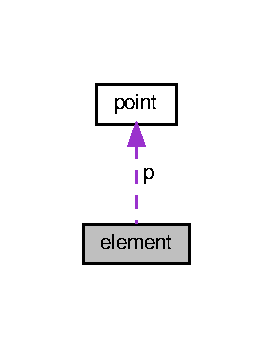
\includegraphics[width=131pt]{structelement__coll__graph}
\end{center}
\end{figure}
\subsubsection*{Data Fields}
\begin{DoxyCompactItemize}
\item 
\mbox{\Hypertarget{structelement_a4dce87d4907bb76f07b538b48567b03a}\label{structelement_a4dce87d4907bb76f07b538b48567b03a}} 
\hyperlink{structpoint}{point} $\ast$ {\bfseries p}
\end{DoxyCompactItemize}


The documentation for this struct was generated from the following file\+:\begin{DoxyCompactItemize}
\item 
clustering\+\_\+goptics.\+c\end{DoxyCompactItemize}

\hypertarget{structempfreq__double__element}{}\subsection{empfreq\+\_\+double\+\_\+element Struct Reference}
\label{structempfreq__double__element}\index{empfreq\+\_\+double\+\_\+element@{empfreq\+\_\+double\+\_\+element}}
\subsubsection*{Data Fields}
\begin{DoxyCompactItemize}
\item 
\mbox{\Hypertarget{structempfreq__double__element_af87b5aceec8f23e1c13f1d818adbb93b}\label{structempfreq__double__element_af87b5aceec8f23e1c13f1d818adbb93b}} 
double {\bfseries freq}
\item 
\mbox{\Hypertarget{structempfreq__double__element_a200ef26955bf526fd4ccb916d797a9c7}\label{structempfreq__double__element_a200ef26955bf526fd4ccb916d797a9c7}} 
int {\bfseries idx}
\end{DoxyCompactItemize}


The documentation for this struct was generated from the following file\+:\begin{DoxyCompactItemize}
\item 
\hyperlink{empirical__frequency_8h}{empirical\+\_\+frequency.\+h}\end{DoxyCompactItemize}

\hypertarget{structempfreq__double__struct}{}\subsection{empfreq\+\_\+double\+\_\+struct Struct Reference}
\label{structempfreq__double__struct}\index{empfreq\+\_\+double\+\_\+struct@{empfreq\+\_\+double\+\_\+struct}}


Collaboration diagram for empfreq\+\_\+double\+\_\+struct\+:\nopagebreak
\begin{figure}[H]
\begin{center}
\leavevmode
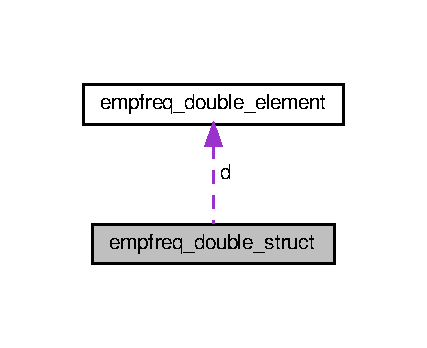
\includegraphics[width=205pt]{structempfreq__double__struct__coll__graph}
\end{center}
\end{figure}
\subsubsection*{Data Fields}
\begin{DoxyCompactItemize}
\item 
\mbox{\Hypertarget{structempfreq__double__struct_a6f6adf630ca569cabaa40dbf8c0e53bf}\label{structempfreq__double__struct_a6f6adf630ca569cabaa40dbf8c0e53bf}} 
\hyperlink{structempfreq__double__element}{empfreq\+\_\+double\+\_\+element} $\ast$ {\bfseries d}
\item 
\mbox{\Hypertarget{structempfreq__double__struct_af590c9b48655f0fc0d02a748fca747c3}\label{structempfreq__double__struct_af590c9b48655f0fc0d02a748fca747c3}} 
int {\bfseries n}
\item 
\mbox{\Hypertarget{structempfreq__double__struct_a6737c6f8768a55f7c7fa56ee567a1888}\label{structempfreq__double__struct_a6737c6f8768a55f7c7fa56ee567a1888}} 
double {\bfseries min}
\item 
\mbox{\Hypertarget{structempfreq__double__struct_afb2643a2e265010b6dfdf24086b8cbfe}\label{structempfreq__double__struct_afb2643a2e265010b6dfdf24086b8cbfe}} 
double \hyperlink{structempfreq__double__struct_afb2643a2e265010b6dfdf24086b8cbfe}{max}
\begin{DoxyCompactList}\small\item\em Min value for index. \end{DoxyCompactList}\item 
\mbox{\Hypertarget{structempfreq__double__struct_a3992dabc855183309cbc0c78c0bf8a35}\label{structempfreq__double__struct_a3992dabc855183309cbc0c78c0bf8a35}} 
int \hyperlink{structempfreq__double__struct_a3992dabc855183309cbc0c78c0bf8a35}{ref\+\_\+counter}
\begin{DoxyCompactList}\small\item\em Max value for index. \end{DoxyCompactList}\end{DoxyCompactItemize}


The documentation for this struct was generated from the following file\+:\begin{DoxyCompactItemize}
\item 
\hyperlink{empirical__frequency_8h}{empirical\+\_\+frequency.\+h}\end{DoxyCompactItemize}

\hypertarget{structempfreq__element}{}\subsection{empfreq\+\_\+element Struct Reference}
\label{structempfreq__element}\index{empfreq\+\_\+element@{empfreq\+\_\+element}}
\subsubsection*{Data Fields}
\begin{DoxyCompactItemize}
\item 
\mbox{\Hypertarget{structempfreq__element_ab424ac77789a11c1b7bc86b5286bba9f}\label{structempfreq__element_ab424ac77789a11c1b7bc86b5286bba9f}} 
int {\bfseries freq}
\item 
\mbox{\Hypertarget{structempfreq__element_a30040ae398445c3524708eb8838a1d16}\label{structempfreq__element_a30040ae398445c3524708eb8838a1d16}} 
int {\bfseries idx}
\end{DoxyCompactItemize}


The documentation for this struct was generated from the following file\+:\begin{DoxyCompactItemize}
\item 
\hyperlink{empirical__frequency_8h}{empirical\+\_\+frequency.\+h}\end{DoxyCompactItemize}

\hypertarget{structempfreq__struct}{}\subsection{empfreq\+\_\+struct Struct Reference}
\label{structempfreq__struct}\index{empfreq\+\_\+struct@{empfreq\+\_\+struct}}


Collaboration diagram for empfreq\+\_\+struct\+:\nopagebreak
\begin{figure}[H]
\begin{center}
\leavevmode
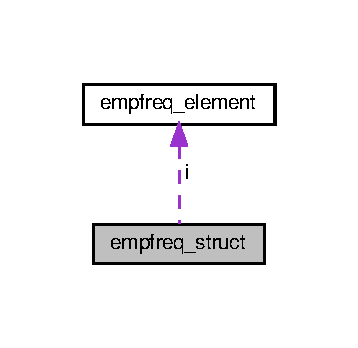
\includegraphics[width=172pt]{structempfreq__struct__coll__graph}
\end{center}
\end{figure}
\subsubsection*{Data Fields}
\begin{DoxyCompactItemize}
\item 
\mbox{\Hypertarget{structempfreq__struct_aea7241e874e94494faf7d65c878a571a}\label{structempfreq__struct_aea7241e874e94494faf7d65c878a571a}} 
\hyperlink{structempfreq__element}{empfreq\+\_\+element} $\ast$ {\bfseries i}
\item 
\mbox{\Hypertarget{structempfreq__struct_a20ee3e8d0078c8022f9201a1218ae495}\label{structempfreq__struct_a20ee3e8d0078c8022f9201a1218ae495}} 
int {\bfseries n}
\item 
\mbox{\Hypertarget{structempfreq__struct_a68c162ae0fc46fe35b6d2510e0e0dc49}\label{structempfreq__struct_a68c162ae0fc46fe35b6d2510e0e0dc49}} 
int {\bfseries min}
\item 
\mbox{\Hypertarget{structempfreq__struct_a8ab2ef9078903277e65b7bf4ff611c2c}\label{structempfreq__struct_a8ab2ef9078903277e65b7bf4ff611c2c}} 
int \hyperlink{structempfreq__struct_a8ab2ef9078903277e65b7bf4ff611c2c}{max}
\begin{DoxyCompactList}\small\item\em Min value for index. \end{DoxyCompactList}\item 
\mbox{\Hypertarget{structempfreq__struct_ac3ad72cff1347a06116940f7f9a85b4e}\label{structempfreq__struct_ac3ad72cff1347a06116940f7f9a85b4e}} 
int \hyperlink{structempfreq__struct_ac3ad72cff1347a06116940f7f9a85b4e}{ref\+\_\+counter}
\begin{DoxyCompactList}\small\item\em Max value for index. \end{DoxyCompactList}\end{DoxyCompactItemize}


The documentation for this struct was generated from the following file\+:\begin{DoxyCompactItemize}
\item 
\hyperlink{empirical__frequency_8h}{empirical\+\_\+frequency.\+h}\end{DoxyCompactItemize}

\hypertarget{structgenetree__struct}{}\subsection{genetree\+\_\+struct Struct Reference}
\label{structgenetree__struct}\index{genetree\+\_\+struct@{genetree\+\_\+struct}}


Collaboration diagram for genetree\+\_\+struct\+:\nopagebreak
\begin{figure}[H]
\begin{center}
\leavevmode
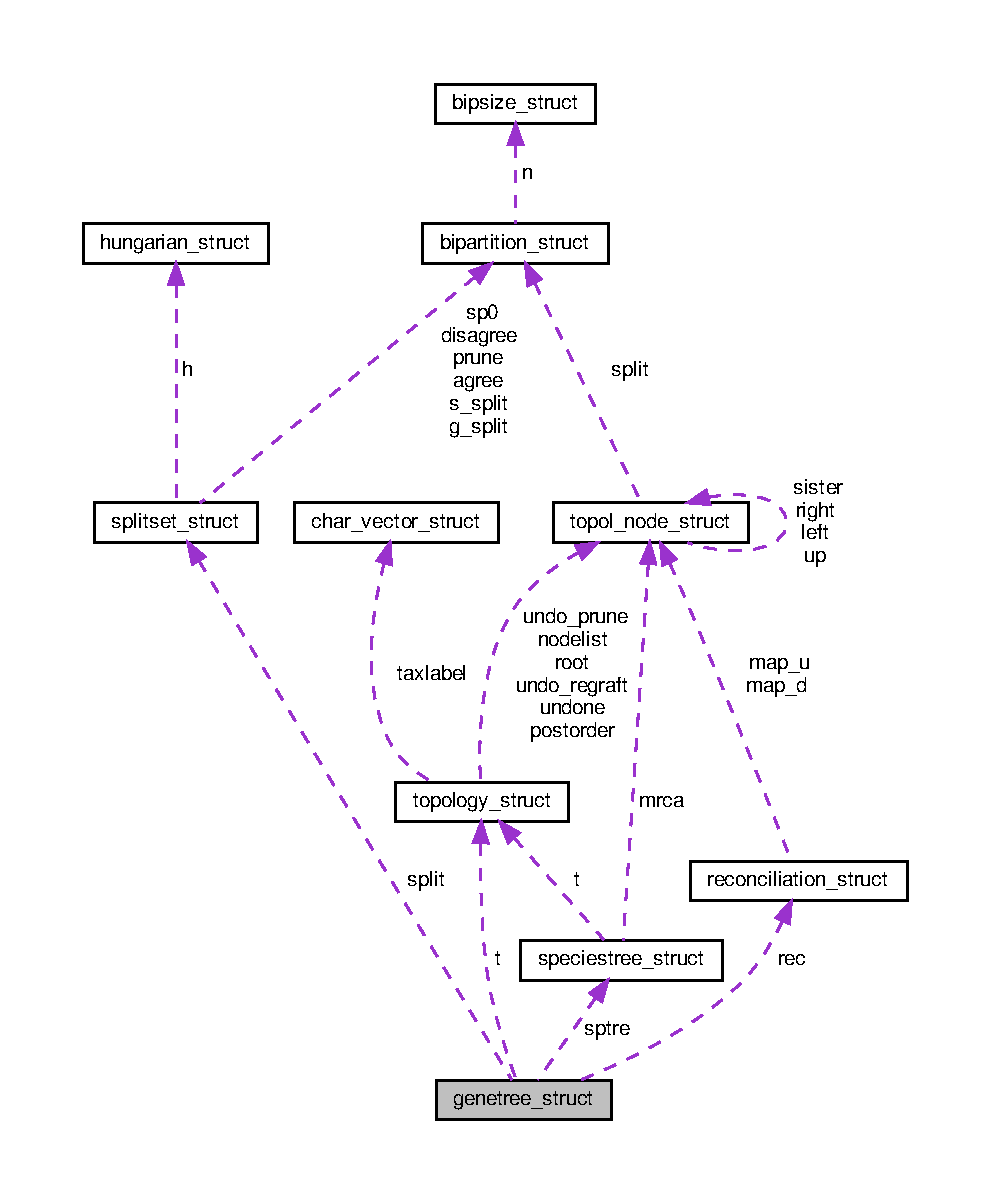
\includegraphics[width=350pt]{structgenetree__struct__coll__graph}
\end{center}
\end{figure}
\subsubsection*{Data Fields}
\begin{DoxyCompactItemize}
\item 
\mbox{\Hypertarget{structgenetree__struct_a477c44458400654d11a902f30c616321}\label{structgenetree__struct_a477c44458400654d11a902f30c616321}} 
\hyperlink{structtopology__struct}{topology} {\bfseries t}
\item 
\mbox{\Hypertarget{structgenetree__struct_a5ba29537e6c9bfb52d69972ab49c9eec}\label{structgenetree__struct_a5ba29537e6c9bfb52d69972ab49c9eec}} 
\hyperlink{structreconciliation__struct}{reconciliation} {\bfseries rec}
\item 
\mbox{\Hypertarget{structgenetree__struct_a63fa84e43aad1603d40dbd37607f66c5}\label{structgenetree__struct_a63fa84e43aad1603d40dbd37607f66c5}} 
\hyperlink{structspeciestree__struct}{speciestree} {\bfseries sptre}
\item 
\mbox{\Hypertarget{structgenetree__struct_a29675629bba123ceffd2d8d54402daad}\label{structgenetree__struct_a29675629bba123ceffd2d8d54402daad}} 
\hyperlink{structsplitset__struct}{splitset} {\bfseries split}
\item 
\mbox{\Hypertarget{structgenetree__struct_abd848a8e8ef0f0bb13aa96f241e87234}\label{structgenetree__struct_abd848a8e8ef0f0bb13aa96f241e87234}} 
int $\ast$ {\bfseries distance}
\item 
\mbox{\Hypertarget{structgenetree__struct_a5d9db824b8191c0c694900d6670b8bf1}\label{structgenetree__struct_a5d9db824b8191c0c694900d6670b8bf1}} 
int $\ast$ {\bfseries minmax}
\item 
\mbox{\Hypertarget{structgenetree__struct_ac996ed5df3cfb4987d10182d342abce8}\label{structgenetree__struct_ac996ed5df3cfb4987d10182d342abce8}} 
int {\bfseries ref\+\_\+counter}
\end{DoxyCompactItemize}


The documentation for this struct was generated from the following file\+:\begin{DoxyCompactItemize}
\item 
\hyperlink{genetree_8h}{genetree.\+h}\end{DoxyCompactItemize}

\hypertarget{structgoptics__cluster__struct}{}\subsection{goptics\+\_\+cluster\+\_\+struct Struct Reference}
\label{structgoptics__cluster__struct}\index{goptics\+\_\+cluster\+\_\+struct@{goptics\+\_\+cluster\+\_\+struct}}


Collaboration diagram for goptics\+\_\+cluster\+\_\+struct\+:\nopagebreak
\begin{figure}[H]
\begin{center}
\leavevmode
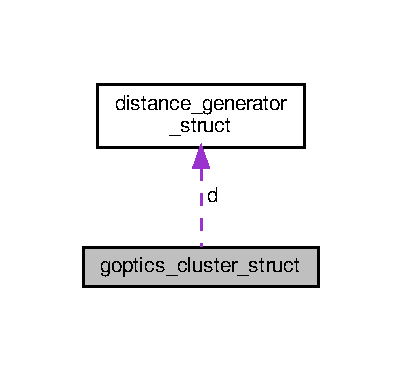
\includegraphics[width=193pt]{structgoptics__cluster__struct__coll__graph}
\end{center}
\end{figure}
\subsubsection*{Data Fields}
\begin{DoxyCompactItemize}
\item 
\mbox{\Hypertarget{structgoptics__cluster__struct_af2b08b4a6fcae92a4a7e1102b3db8cda}\label{structgoptics__cluster__struct_af2b08b4a6fcae92a4a7e1102b3db8cda}} 
int $\ast$ {\bfseries Va\+\_\+i}
\item 
\mbox{\Hypertarget{structgoptics__cluster__struct_aa40c4cbb8bec4469983e601e5f92211f}\label{structgoptics__cluster__struct_aa40c4cbb8bec4469983e601e5f92211f}} 
int $\ast$ {\bfseries Va\+\_\+n}
\item 
\mbox{\Hypertarget{structgoptics__cluster__struct_a06e88207f36a3d00c9960a51323f1689}\label{structgoptics__cluster__struct_a06e88207f36a3d00c9960a51323f1689}} 
double {\bfseries epsilon}
\item 
\mbox{\Hypertarget{structgoptics__cluster__struct_a826183dec61c805418d252ee11ca8a01}\label{structgoptics__cluster__struct_a826183dec61c805418d252ee11ca8a01}} 
int {\bfseries min\+\_\+points}
\item 
\mbox{\Hypertarget{structgoptics__cluster__struct_a4f3b38d0925a9e91d6019d05ac9c20c8}\label{structgoptics__cluster__struct_a4f3b38d0925a9e91d6019d05ac9c20c8}} 
int {\bfseries num\+\_\+edges}
\item 
\mbox{\Hypertarget{structgoptics__cluster__struct_ac7a646909a8d907ae337ee7a0aa64939}\label{structgoptics__cluster__struct_ac7a646909a8d907ae337ee7a0aa64939}} 
int {\bfseries n\+\_\+clusters}
\item 
\mbox{\Hypertarget{structgoptics__cluster__struct_a618783321abf976838bdab3a390fd851}\label{structgoptics__cluster__struct_a618783321abf976838bdab3a390fd851}} 
int $\ast$ {\bfseries order}
\item 
\mbox{\Hypertarget{structgoptics__cluster__struct_a827a5ef6d6212589e19dfa822956b4da}\label{structgoptics__cluster__struct_a827a5ef6d6212589e19dfa822956b4da}} 
int {\bfseries n\+\_\+order}
\item 
\mbox{\Hypertarget{structgoptics__cluster__struct_ac6a9d0632a283c3db978cc1639025dab}\label{structgoptics__cluster__struct_ac6a9d0632a283c3db978cc1639025dab}} 
int $\ast$ {\bfseries cluster}
\item 
\mbox{\Hypertarget{structgoptics__cluster__struct_a669d1e67fa3f0daf68725d60c812d038}\label{structgoptics__cluster__struct_a669d1e67fa3f0daf68725d60c812d038}} 
double $\ast$ {\bfseries core\+\_\+distance}
\item 
\mbox{\Hypertarget{structgoptics__cluster__struct_a49a668329b0f258244aec560dee713a5}\label{structgoptics__cluster__struct_a49a668329b0f258244aec560dee713a5}} 
double $\ast$ {\bfseries reach\+\_\+distance}
\item 
\mbox{\Hypertarget{structgoptics__cluster__struct_afb23461667cc643aa9609f50d5f7c95c}\label{structgoptics__cluster__struct_afb23461667cc643aa9609f50d5f7c95c}} 
double {\bfseries max\+\_\+distance}
\item 
\mbox{\Hypertarget{structgoptics__cluster__struct_aed579d02083c6af4f9d87d1d5d3eac61}\label{structgoptics__cluster__struct_aed579d02083c6af4f9d87d1d5d3eac61}} 
\hyperlink{lowlevel_8h_a97a80ca1602ebf2303258971a2c938e2}{bool} $\ast$ {\bfseries core}
\item 
\mbox{\Hypertarget{structgoptics__cluster__struct_a0a4fe7cba7d345305635721c57091425}\label{structgoptics__cluster__struct_a0a4fe7cba7d345305635721c57091425}} 
void $\ast$ {\bfseries Ea}
\item 
\mbox{\Hypertarget{structgoptics__cluster__struct_a1efe741cee0d65d9c2faea8be1fccdff}\label{structgoptics__cluster__struct_a1efe741cee0d65d9c2faea8be1fccdff}} 
void $\ast$ {\bfseries heap}
\item 
\mbox{\Hypertarget{structgoptics__cluster__struct_a9c0395bfbb20960478d873df23e179f4}\label{structgoptics__cluster__struct_a9c0395bfbb20960478d873df23e179f4}} 
void $\ast$ {\bfseries points}
\item 
\mbox{\Hypertarget{structgoptics__cluster__struct_ade33930b1c6e266735b8413a7c98bc9d}\label{structgoptics__cluster__struct_ade33930b1c6e266735b8413a7c98bc9d}} 
double {\bfseries timing\+\_\+secs}
\item 
\mbox{\Hypertarget{structgoptics__cluster__struct_a6bd1c762f8424341fd97867fe95de77f}\label{structgoptics__cluster__struct_a6bd1c762f8424341fd97867fe95de77f}} 
\hyperlink{structdistance__generator__struct}{distance\+\_\+generator} {\bfseries d}
\end{DoxyCompactItemize}


The documentation for this struct was generated from the following file\+:\begin{DoxyCompactItemize}
\item 
\hyperlink{clustering__goptics_8h}{clustering\+\_\+goptics.\+h}\end{DoxyCompactItemize}

\hypertarget{structhashtable__item__struct}{}\subsection{hashtable\+\_\+item\+\_\+struct Struct Reference}
\label{structhashtable__item__struct}\index{hashtable\+\_\+item\+\_\+struct@{hashtable\+\_\+item\+\_\+struct}}


key/value pair for hash table  




{\ttfamily \#include $<$hashtable.\+h$>$}

\subsubsection*{Data Fields}
\begin{DoxyCompactItemize}
\item 
\mbox{\Hypertarget{structhashtable__item__struct_a69e66635eb50b52a33f677684e9e9ea8}\label{structhashtable__item__struct_a69e66635eb50b52a33f677684e9e9ea8}} 
char $\ast$ \hyperlink{structhashtable__item__struct_a69e66635eb50b52a33f677684e9e9ea8}{key}
\begin{DoxyCompactList}\small\item\em String (vector of char). \end{DoxyCompactList}\item 
\mbox{\Hypertarget{structhashtable__item__struct_adf2cf000a4deead466a3d40e99a4c913}\label{structhashtable__item__struct_adf2cf000a4deead466a3d40e99a4c913}} 
int \hyperlink{structhashtable__item__struct_adf2cf000a4deead466a3d40e99a4c913}{value}
\begin{DoxyCompactList}\small\item\em Integer (position in vector where \hyperlink{structhashtable__item__struct_a69e66635eb50b52a33f677684e9e9ea8}{hashtable\+\_\+item\+\_\+struct\+::key} can be found) \end{DoxyCompactList}\end{DoxyCompactItemize}


\subsubsection{Detailed Description}
key/value pair for hash table 

The documentation for this struct was generated from the following file\+:\begin{DoxyCompactItemize}
\item 
\hyperlink{hashtable_8h}{hashtable.\+h}\end{DoxyCompactItemize}

\hypertarget{structhashtable__struct}{}\subsection{hashtable\+\_\+struct Struct Reference}
\label{structhashtable__struct}\index{hashtable\+\_\+struct@{hashtable\+\_\+struct}}


Hash table (vector indexed by strings).  




{\ttfamily \#include $<$hashtable.\+h$>$}



Collaboration diagram for hashtable\+\_\+struct\+:\nopagebreak
\begin{figure}[H]
\begin{center}
\leavevmode
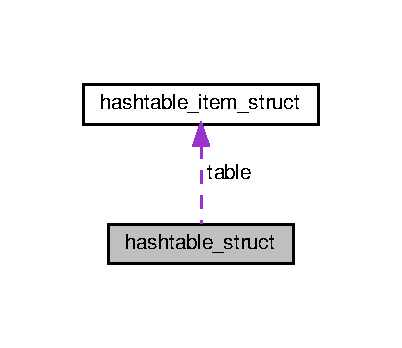
\includegraphics[width=193pt]{structhashtable__struct__coll__graph}
\end{center}
\end{figure}
\subsubsection*{Data Fields}
\begin{DoxyCompactItemize}
\item 
\mbox{\Hypertarget{structhashtable__struct_a0fb42778e1d783631e499751ba367b06}\label{structhashtable__struct_a0fb42778e1d783631e499751ba367b06}} 
int \hyperlink{structhashtable__struct_a0fb42778e1d783631e499751ba367b06}{size}
\begin{DoxyCompactList}\small\item\em Table size. \end{DoxyCompactList}\item 
\mbox{\Hypertarget{structhashtable__struct_a861882ffbcb186d96f90b82d1dc39f40}\label{structhashtable__struct_a861882ffbcb186d96f90b82d1dc39f40}} 
int \hyperlink{structhashtable__struct_a861882ffbcb186d96f90b82d1dc39f40}{probelength}
\begin{DoxyCompactList}\small\item\em Number of collisions before empty slot is found. \end{DoxyCompactList}\item 
\mbox{\Hypertarget{structhashtable__struct_ae77d63df7a927e68de61d431d5bc0ddc}\label{structhashtable__struct_ae77d63df7a927e68de61d431d5bc0ddc}} 
uint32\+\_\+t \hyperlink{structhashtable__struct_ae77d63df7a927e68de61d431d5bc0ddc}{h}
\begin{DoxyCompactList}\small\item\em Value set by hash(). Used in hash1() and hash2() to avoid calling hash() again. \end{DoxyCompactList}\item 
\mbox{\Hypertarget{structhashtable__struct_a563092db06242cc9e284954b01c3b133}\label{structhashtable__struct_a563092db06242cc9e284954b01c3b133}} 
uint32\+\_\+t \hyperlink{structhashtable__struct_a563092db06242cc9e284954b01c3b133}{a1}
\begin{DoxyCompactList}\small\item\em Random values used in hash functions. \end{DoxyCompactList}\item 
\mbox{\Hypertarget{structhashtable__struct_af183bbfbf1e17f0f82ac0ea623f383e3}\label{structhashtable__struct_af183bbfbf1e17f0f82ac0ea623f383e3}} 
uint32\+\_\+t \hyperlink{structhashtable__struct_af183bbfbf1e17f0f82ac0ea623f383e3}{a2}
\begin{DoxyCompactList}\small\item\em Random values used in hash functions. \end{DoxyCompactList}\item 
\mbox{\Hypertarget{structhashtable__struct_a3d65fc5f5625a3c950ae177599c1a4dc}\label{structhashtable__struct_a3d65fc5f5625a3c950ae177599c1a4dc}} 
uint32\+\_\+t \hyperlink{structhashtable__struct_a3d65fc5f5625a3c950ae177599c1a4dc}{b1}
\begin{DoxyCompactList}\small\item\em Random values used in hash functions. \end{DoxyCompactList}\item 
\mbox{\Hypertarget{structhashtable__struct_a7c912d95360bc525d15b5a7cd7906ce3}\label{structhashtable__struct_a7c912d95360bc525d15b5a7cd7906ce3}} 
uint32\+\_\+t \hyperlink{structhashtable__struct_a7c912d95360bc525d15b5a7cd7906ce3}{b2}
\begin{DoxyCompactList}\small\item\em Random values used in hash functions. \end{DoxyCompactList}\item 
\mbox{\Hypertarget{structhashtable__struct_af1b180f0885b6077b7eeb60fa8267058}\label{structhashtable__struct_af1b180f0885b6077b7eeb60fa8267058}} 
uint32\+\_\+t \hyperlink{structhashtable__struct_af1b180f0885b6077b7eeb60fa8267058}{P}
\begin{DoxyCompactList}\small\item\em Random values used in hash functions. \end{DoxyCompactList}\item 
\mbox{\Hypertarget{structhashtable__struct_ae8753bc6e120a945558de12c7fc53fd6}\label{structhashtable__struct_ae8753bc6e120a945558de12c7fc53fd6}} 
\hyperlink{structhashtable__item__struct}{hashtable\+\_\+item} $\ast$ \hyperlink{structhashtable__struct_ae8753bc6e120a945558de12c7fc53fd6}{table}
\begin{DoxyCompactList}\small\item\em Vector with key/value pairs. \end{DoxyCompactList}\item 
\mbox{\Hypertarget{structhashtable__struct_a83abeb291046d5560c2e1612c70c86d0}\label{structhashtable__struct_a83abeb291046d5560c2e1612c70c86d0}} 
int \hyperlink{structhashtable__struct_a83abeb291046d5560c2e1612c70c86d0}{ref\+\_\+counter}
\begin{DoxyCompactList}\small\item\em Counter of how many external references (structures sharing this hashtable) to avoid deletion. \end{DoxyCompactList}\end{DoxyCompactItemize}


\subsubsection{Detailed Description}
Hash table (vector indexed by strings). 

The documentation for this struct was generated from the following file\+:\begin{DoxyCompactItemize}
\item 
\hyperlink{hashtable_8h}{hashtable.\+h}\end{DoxyCompactItemize}

\hypertarget{structhll__estimate__s}{}\subsection{hll\+\_\+estimate\+\_\+s Struct Reference}
\label{structhll__estimate__s}\index{hll\+\_\+estimate\+\_\+s@{hll\+\_\+estimate\+\_\+s}}


{\ttfamily \#include $<$hll.\+h$>$}

\subsubsection*{Data Fields}
\begin{DoxyCompactItemize}
\item 
\mbox{\Hypertarget{structhll__estimate__s_ace8957a5abbf4554e722159d2933e6b9}\label{structhll__estimate__s_ace8957a5abbf4554e722159d2933e6b9}} 
double {\bfseries alpha}
\item 
uint16\+\_\+t \hyperlink{structhll__estimate__s_a6124b7e8334b402dc3f7d2855642767b}{n\+\_\+buckets}
\item 
uint16\+\_\+t \hyperlink{structhll__estimate__s_a0c7a468e18e2b31792f28f300dddc83f}{n\+\_\+empty\+\_\+buckets}
\item 
uint64\+\_\+t \hyperlink{structhll__estimate__s_a6d651ad449a38baa6a5a47d9361155d6}{estimate}
\item 
uint64\+\_\+t \hyperlink{structhll__estimate__s_a44153272b5b7925bbe518645a3f146d0}{hll\+\_\+estimate}
\item 
uint64\+\_\+t \hyperlink{structhll__estimate__s_acfa1e2f8075ca50adcbc6cfec4a86e28}{small\+\_\+range\+\_\+estimate}
\item 
uint64\+\_\+t \hyperlink{structhll__estimate__s_ae6e8601592aec248a11f378e1b946f60}{large\+\_\+range\+\_\+estimate}
\end{DoxyCompactItemize}


\subsubsection{Detailed Description}
Estimation result data structure 

\subsubsection{Field Documentation}
\mbox{\Hypertarget{structhll__estimate__s_a6124b7e8334b402dc3f7d2855642767b}\label{structhll__estimate__s_a6124b7e8334b402dc3f7d2855642767b}} 
\index{hll\+\_\+estimate\+\_\+s@{hll\+\_\+estimate\+\_\+s}!n\+\_\+buckets@{n\+\_\+buckets}}
\index{n\+\_\+buckets@{n\+\_\+buckets}!hll\+\_\+estimate\+\_\+s@{hll\+\_\+estimate\+\_\+s}}
\paragraph{\texorpdfstring{n\+\_\+buckets}{n\_buckets}}
{\footnotesize\ttfamily uint16\+\_\+t hll\+\_\+estimate\+\_\+s\+::n\+\_\+buckets}

Alpha \mbox{\Hypertarget{structhll__estimate__s_a0c7a468e18e2b31792f28f300dddc83f}\label{structhll__estimate__s_a0c7a468e18e2b31792f28f300dddc83f}} 
\index{hll\+\_\+estimate\+\_\+s@{hll\+\_\+estimate\+\_\+s}!n\+\_\+empty\+\_\+buckets@{n\+\_\+empty\+\_\+buckets}}
\index{n\+\_\+empty\+\_\+buckets@{n\+\_\+empty\+\_\+buckets}!hll\+\_\+estimate\+\_\+s@{hll\+\_\+estimate\+\_\+s}}
\paragraph{\texorpdfstring{n\+\_\+empty\+\_\+buckets}{n\_empty\_buckets}}
{\footnotesize\ttfamily uint16\+\_\+t hll\+\_\+estimate\+\_\+s\+::n\+\_\+empty\+\_\+buckets}

Number of buckets \mbox{\Hypertarget{structhll__estimate__s_a6d651ad449a38baa6a5a47d9361155d6}\label{structhll__estimate__s_a6d651ad449a38baa6a5a47d9361155d6}} 
\index{hll\+\_\+estimate\+\_\+s@{hll\+\_\+estimate\+\_\+s}!estimate@{estimate}}
\index{estimate@{estimate}!hll\+\_\+estimate\+\_\+s@{hll\+\_\+estimate\+\_\+s}}
\paragraph{\texorpdfstring{estimate}{estimate}}
{\footnotesize\ttfamily uint64\+\_\+t hll\+\_\+estimate\+\_\+s\+::estimate}

Number of empty buckets \mbox{\Hypertarget{structhll__estimate__s_a44153272b5b7925bbe518645a3f146d0}\label{structhll__estimate__s_a44153272b5b7925bbe518645a3f146d0}} 
\index{hll\+\_\+estimate\+\_\+s@{hll\+\_\+estimate\+\_\+s}!hll\+\_\+estimate@{hll\+\_\+estimate}}
\index{hll\+\_\+estimate@{hll\+\_\+estimate}!hll\+\_\+estimate\+\_\+s@{hll\+\_\+estimate\+\_\+s}}
\paragraph{\texorpdfstring{hll\+\_\+estimate}{hll\_estimate}}
{\footnotesize\ttfamily uint64\+\_\+t hll\+\_\+estimate\+\_\+s\+::hll\+\_\+estimate}

Final estimated cardinality \mbox{\Hypertarget{structhll__estimate__s_acfa1e2f8075ca50adcbc6cfec4a86e28}\label{structhll__estimate__s_acfa1e2f8075ca50adcbc6cfec4a86e28}} 
\index{hll\+\_\+estimate\+\_\+s@{hll\+\_\+estimate\+\_\+s}!small\+\_\+range\+\_\+estimate@{small\+\_\+range\+\_\+estimate}}
\index{small\+\_\+range\+\_\+estimate@{small\+\_\+range\+\_\+estimate}!hll\+\_\+estimate\+\_\+s@{hll\+\_\+estimate\+\_\+s}}
\paragraph{\texorpdfstring{small\+\_\+range\+\_\+estimate}{small\_range\_estimate}}
{\footnotesize\ttfamily uint64\+\_\+t hll\+\_\+estimate\+\_\+s\+::small\+\_\+range\+\_\+estimate}

H\+LL estimated cardinaloty, before any correction \mbox{\Hypertarget{structhll__estimate__s_ae6e8601592aec248a11f378e1b946f60}\label{structhll__estimate__s_ae6e8601592aec248a11f378e1b946f60}} 
\index{hll\+\_\+estimate\+\_\+s@{hll\+\_\+estimate\+\_\+s}!large\+\_\+range\+\_\+estimate@{large\+\_\+range\+\_\+estimate}}
\index{large\+\_\+range\+\_\+estimate@{large\+\_\+range\+\_\+estimate}!hll\+\_\+estimate\+\_\+s@{hll\+\_\+estimate\+\_\+s}}
\paragraph{\texorpdfstring{large\+\_\+range\+\_\+estimate}{large\_range\_estimate}}
{\footnotesize\ttfamily uint64\+\_\+t hll\+\_\+estimate\+\_\+s\+::large\+\_\+range\+\_\+estimate}

Small range estimated cardinality 

The documentation for this struct was generated from the following file\+:\begin{DoxyCompactItemize}
\item 
\hyperlink{hll_8h}{hll.\+h}\end{DoxyCompactItemize}

\hypertarget{structhll__s}{}\subsection{hll\+\_\+s Struct Reference}
\label{structhll__s}\index{hll\+\_\+s@{hll\+\_\+s}}
\subsubsection*{Data Fields}
\begin{DoxyCompactItemize}
\item 
\mbox{\Hypertarget{structhll__s_a5b24831053600f820bfed2ec2fe3f045}\label{structhll__s_a5b24831053600f820bfed2ec2fe3f045}} 
double {\bfseries alpha}
\item 
\mbox{\Hypertarget{structhll__s_aea5f44ec6e0d4a5523c12ab903ddc69e}\label{structhll__s_aea5f44ec6e0d4a5523c12ab903ddc69e}} 
size\+\_\+t {\bfseries n\+\_\+buckets}
\item 
\mbox{\Hypertarget{structhll__s_a0991b26d77fcff7388e6f251ca0e1025}\label{structhll__s_a0991b26d77fcff7388e6f251ca0e1025}} 
uint8\+\_\+t $\ast$ {\bfseries buckets}
\item 
\mbox{\Hypertarget{structhll__s_ac90d6c814a73bc480e7e6e84183267bf}\label{structhll__s_ac90d6c814a73bc480e7e6e84183267bf}} 
\hyperlink{hll_8h_a4810b852ed49962affc0136b06664f06}{hll\+\_\+hash\+\_\+function\+\_\+t} {\bfseries hash\+\_\+function}
\end{DoxyCompactItemize}


The documentation for this struct was generated from the following file\+:\begin{DoxyCompactItemize}
\item 
hll.\+c\end{DoxyCompactItemize}

\hypertarget{structhungarian__struct}{}\subsection{hungarian\+\_\+struct Struct Reference}
\label{structhungarian__struct}\index{hungarian\+\_\+struct@{hungarian\+\_\+struct}}
\subsubsection*{Data Fields}
\begin{DoxyCompactItemize}
\item 
\mbox{\Hypertarget{structhungarian__struct_a035c909caa99385d7de0a3121930ea97}\label{structhungarian__struct_a035c909caa99385d7de0a3121930ea97}} 
int $\ast$$\ast$ {\bfseries cost}
\item 
\mbox{\Hypertarget{structhungarian__struct_add5775a6b09229dafbf70064ee507f8a}\label{structhungarian__struct_add5775a6b09229dafbf70064ee507f8a}} 
int \hyperlink{structhungarian__struct_add5775a6b09229dafbf70064ee507f8a}{size}
\begin{DoxyCompactList}\small\item\em cost matrix \end{DoxyCompactList}\item 
\mbox{\Hypertarget{structhungarian__struct_aac743e34a5477355c52bf0385a1a834a}\label{structhungarian__struct_aac743e34a5477355c52bf0385a1a834a}} 
int \hyperlink{structhungarian__struct_aac743e34a5477355c52bf0385a1a834a}{initial\+\_\+cost}
\begin{DoxyCompactList}\small\item\em assignment size. Cost is a square matrix, so size should be an overestimate where \char`\"{}missing\char`\"{} nodes are added w/ cost zero \end{DoxyCompactList}\item 
\mbox{\Hypertarget{structhungarian__struct_a585c79fc76d76c173a9b9ad93fb4a3a3}\label{structhungarian__struct_a585c79fc76d76c173a9b9ad93fb4a3a3}} 
int \hyperlink{structhungarian__struct_a585c79fc76d76c173a9b9ad93fb4a3a3}{final\+\_\+cost}
\begin{DoxyCompactList}\small\item\em sum of lowest input cost values for each column. The hungarian method rescales them so that minimum per column is zero \end{DoxyCompactList}\item 
\mbox{\Hypertarget{structhungarian__struct_ad1aa7dc6487faaa08c5412aca4443f96}\label{structhungarian__struct_ad1aa7dc6487faaa08c5412aca4443f96}} 
int $\ast$ \hyperlink{structhungarian__struct_ad1aa7dc6487faaa08c5412aca4443f96}{col\+\_\+mate}
\begin{DoxyCompactList}\small\item\em our final cost is on rescaled cost matrix, therefore to restore the \char`\"{}classical\char`\"{} optimal cost one should sum it with initial\+\_\+cost \end{DoxyCompactList}\item 
\mbox{\Hypertarget{structhungarian__struct_a3a1148ae045f0d79d9cf0f9af9ee672c}\label{structhungarian__struct_a3a1148ae045f0d79d9cf0f9af9ee672c}} 
int $\ast$ {\bfseries unchosen\+\_\+row}
\item 
\mbox{\Hypertarget{structhungarian__struct_af2cbec1d573cd8e4ab960c9dff026e3a}\label{structhungarian__struct_af2cbec1d573cd8e4ab960c9dff026e3a}} 
int $\ast$ {\bfseries slack\+\_\+row}
\item 
\mbox{\Hypertarget{structhungarian__struct_ae933db937fbf3cf6e0fec730cba07431}\label{structhungarian__struct_ae933db937fbf3cf6e0fec730cba07431}} 
int $\ast$ {\bfseries row\+\_\+mate}
\item 
\mbox{\Hypertarget{structhungarian__struct_a6120eedc80441baa440621920d9d731f}\label{structhungarian__struct_a6120eedc80441baa440621920d9d731f}} 
int $\ast$ {\bfseries parent\+\_\+row}
\item 
\mbox{\Hypertarget{structhungarian__struct_a7bacee8475c3d90d879d7b31aa4d1af9}\label{structhungarian__struct_a7bacee8475c3d90d879d7b31aa4d1af9}} 
double $\ast$$\ast$ \hyperlink{structhungarian__struct_a7bacee8475c3d90d879d7b31aa4d1af9}{dcost}
\begin{DoxyCompactList}\small\item\em col\+\_\+mate\mbox{[}row\mbox{]} with column match for row \end{DoxyCompactList}\item 
\mbox{\Hypertarget{structhungarian__struct_a56543be8800d38b356c8832b3cb0d3f0}\label{structhungarian__struct_a56543be8800d38b356c8832b3cb0d3f0}} 
double {\bfseries initial\+\_\+dcost}
\item 
\mbox{\Hypertarget{structhungarian__struct_a20d0397e071c5c2078e5d5787a03417d}\label{structhungarian__struct_a20d0397e071c5c2078e5d5787a03417d}} 
double {\bfseries final\+\_\+dcost}
\item 
\mbox{\Hypertarget{structhungarian__struct_a9620ca241d63fadd87189bf117bad71a}\label{structhungarian__struct_a9620ca241d63fadd87189bf117bad71a}} 
double $\ast$ \hyperlink{structhungarian__struct_a9620ca241d63fadd87189bf117bad71a}{row\+\_\+dec\+\_\+d}
\begin{DoxyCompactList}\small\item\em costs when working with float numbers instead of integers \end{DoxyCompactList}\item 
\mbox{\Hypertarget{structhungarian__struct_a664fb941cbe92edac9b53b3a73ab2bcf}\label{structhungarian__struct_a664fb941cbe92edac9b53b3a73ab2bcf}} 
double $\ast$ {\bfseries col\+\_\+inc\+\_\+d}
\item 
\mbox{\Hypertarget{structhungarian__struct_ab950c557f9dfff879eb5ee24e6aacd02}\label{structhungarian__struct_ab950c557f9dfff879eb5ee24e6aacd02}} 
double $\ast$ {\bfseries slack\+\_\+d}
\item 
\mbox{\Hypertarget{structhungarian__struct_a0800735b749c19f173bc7fcd308120a6}\label{structhungarian__struct_a0800735b749c19f173bc7fcd308120a6}} 
int $\ast$ {\bfseries row\+\_\+dec}
\item 
\mbox{\Hypertarget{structhungarian__struct_a935949b5feabfb7ec7328c159c7a6bb6}\label{structhungarian__struct_a935949b5feabfb7ec7328c159c7a6bb6}} 
int $\ast$ {\bfseries col\+\_\+inc}
\item 
\mbox{\Hypertarget{structhungarian__struct_ae000f8eb99f06115d85943377e0bbf97}\label{structhungarian__struct_ae000f8eb99f06115d85943377e0bbf97}} 
int $\ast$ {\bfseries slack}
\item 
\mbox{\Hypertarget{structhungarian__struct_ac1f3d3ba3885b39457c4fe89b3fc0b81}\label{structhungarian__struct_ac1f3d3ba3885b39457c4fe89b3fc0b81}} 
\hyperlink{lowlevel_8h_a97a80ca1602ebf2303258971a2c938e2}{bool} {\bfseries is\+\_\+double}
\end{DoxyCompactItemize}


The documentation for this struct was generated from the following file\+:\begin{DoxyCompactItemize}
\item 
\hyperlink{lowlevel_8h}{lowlevel.\+h}\end{DoxyCompactItemize}

\hypertarget{structkmer__params__struct}{}\subsection{kmer\+\_\+params\+\_\+struct Struct Reference}
\label{structkmer__params__struct}\index{kmer\+\_\+params\+\_\+struct@{kmer\+\_\+params\+\_\+struct}}
\subsubsection*{Data Fields}
\begin{DoxyCompactItemize}
\item 
\mbox{\Hypertarget{structkmer__params__struct_af80e5776dcc1f7f4dfae6c7b79b595b8}\label{structkmer__params__struct_af80e5776dcc1f7f4dfae6c7b79b595b8}} 
uint64\+\_\+t {\bfseries mask1} \mbox{[}7\mbox{]}
\item 
\mbox{\Hypertarget{structkmer__params__struct_aaa66a8435750e8ab831b0e7a1b0c3e70}\label{structkmer__params__struct_aaa66a8435750e8ab831b0e7a1b0c3e70}} 
uint64\+\_\+t {\bfseries mask2} \mbox{[}7\mbox{]}
\item 
\mbox{\Hypertarget{structkmer__params__struct_aab6dd54402fc241b6ef822e77228b1b7}\label{structkmer__params__struct_aab6dd54402fc241b6ef822e77228b1b7}} 
uint8\+\_\+t {\bfseries n1}
\item 
\mbox{\Hypertarget{structkmer__params__struct_a4f6a79e0e4646fcbf2b05c39a6b9831a}\label{structkmer__params__struct_a4f6a79e0e4646fcbf2b05c39a6b9831a}} 
uint8\+\_\+t {\bfseries n2}
\item 
\mbox{\Hypertarget{structkmer__params__struct_a575a2bacb5248cdd4f22c29042941352}\label{structkmer__params__struct_a575a2bacb5248cdd4f22c29042941352}} 
uint8\+\_\+t {\bfseries shift1} \mbox{[}7\mbox{]}
\item 
\mbox{\Hypertarget{structkmer__params__struct_a1907bcc459d99eb614c37bf5211907e2}\label{structkmer__params__struct_a1907bcc459d99eb614c37bf5211907e2}} 
uint8\+\_\+t {\bfseries shift2} \mbox{[}7\mbox{]}
\item 
\mbox{\Hypertarget{structkmer__params__struct_af55607c5032ea68b776b00e5c680adc8}\label{structkmer__params__struct_af55607c5032ea68b776b00e5c680adc8}} 
uint8\+\_\+t {\bfseries size} \mbox{[}14\mbox{]}
\item 
\mbox{\Hypertarget{structkmer__params__struct_ad1cee61f4361f4c90e96d33dd76ee59e}\label{structkmer__params__struct_ad1cee61f4361f4c90e96d33dd76ee59e}} 
uint8\+\_\+t {\bfseries nbytes} \mbox{[}14\mbox{]}
\item 
\mbox{\Hypertarget{structkmer__params__struct_a77f5eb77679070522873aaa03a755556}\label{structkmer__params__struct_a77f5eb77679070522873aaa03a755556}} 
uint32\+\_\+t {\bfseries seed} \mbox{[}14\mbox{]}
\item 
\mbox{\Hypertarget{structkmer__params__struct_a5ea059ef3fcd9b26afc606f5dcc56f11}\label{structkmer__params__struct_a5ea059ef3fcd9b26afc606f5dcc56f11}} 
uint64\+\_\+t($\ast$ {\bfseries hashfunction} )(const void $\ast$, const size\+\_\+t, const uint32\+\_\+t)
\item 
\mbox{\Hypertarget{structkmer__params__struct_a69d70574b05a23738d7bc513506a5f55}\label{structkmer__params__struct_a69d70574b05a23738d7bc513506a5f55}} 
int {\bfseries dense}
\item 
\mbox{\Hypertarget{structkmer__params__struct_a6802863a0456220728dbc871b3231f41}\label{structkmer__params__struct_a6802863a0456220728dbc871b3231f41}} 
int \hyperlink{structkmer__params__struct_a6802863a0456220728dbc871b3231f41}{kmer\+\_\+class\+\_\+mode}
\begin{DoxyCompactList}\small\item\em 4bits per base or 2bits or 1 bit (GC content) \end{DoxyCompactList}\item 
\mbox{\Hypertarget{structkmer__params__struct_a55fd86af1c62c75de5e275d69a83bcc7}\label{structkmer__params__struct_a55fd86af1c62c75de5e275d69a83bcc7}} 
int {\bfseries ref\+\_\+counter}
\end{DoxyCompactItemize}


The documentation for this struct was generated from the following file\+:\begin{DoxyCompactItemize}
\item 
\hyperlink{kmerhash_8h}{kmerhash.\+h}\end{DoxyCompactItemize}

\hypertarget{structkmerhash__struct}{}\subsection{kmerhash\+\_\+struct Struct Reference}
\label{structkmerhash__struct}\index{kmerhash\+\_\+struct@{kmerhash\+\_\+struct}}


Collaboration diagram for kmerhash\+\_\+struct\+:\nopagebreak
\begin{figure}[H]
\begin{center}
\leavevmode
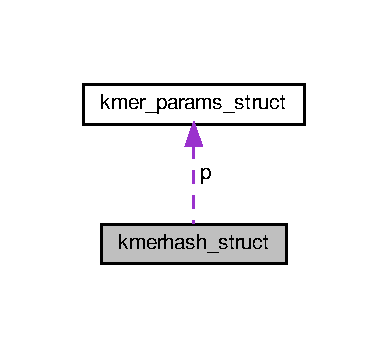
\includegraphics[width=186pt]{structkmerhash__struct__coll__graph}
\end{center}
\end{figure}
\subsubsection*{Data Fields}
\begin{DoxyCompactItemize}
\item 
\mbox{\Hypertarget{structkmerhash__struct_a23892ad222dad6a79273beca81e995c0}\label{structkmerhash__struct_a23892ad222dad6a79273beca81e995c0}} 
\hyperlink{structkmer__params__struct}{kmer\+\_\+params} {\bfseries p}
\item 
\mbox{\Hypertarget{structkmerhash__struct_aa3c9693685126b991f164cec4b4dd7bb}\label{structkmerhash__struct_aa3c9693685126b991f164cec4b4dd7bb}} 
uint64\+\_\+t $\ast$ {\bfseries forward}
\item 
\mbox{\Hypertarget{structkmerhash__struct_ad902710026c95bd26bd0c1b80d7fcaa3}\label{structkmerhash__struct_ad902710026c95bd26bd0c1b80d7fcaa3}} 
uint64\+\_\+t $\ast$ {\bfseries reverse}
\item 
\mbox{\Hypertarget{structkmerhash__struct_a01038ae0a80679f16193b0fefd307463}\label{structkmerhash__struct_a01038ae0a80679f16193b0fefd307463}} 
uint64\+\_\+t $\ast$ {\bfseries hash}
\item 
\mbox{\Hypertarget{structkmerhash__struct_aadebb3ec22d087df6e871c97226457e9}\label{structkmerhash__struct_aadebb3ec22d087df6e871c97226457e9}} 
uint64\+\_\+t $\ast$ {\bfseries kmer}
\item 
\mbox{\Hypertarget{structkmerhash__struct_a7b70ba55ef5a3b80903d066bf5e541b6}\label{structkmerhash__struct_a7b70ba55ef5a3b80903d066bf5e541b6}} 
int \hyperlink{structkmerhash__struct_a7b70ba55ef5a3b80903d066bf5e541b6}{n\+\_\+hash}
\begin{DoxyCompactList}\small\item\em hash = 4mer, 8mer, etc. hashed ; kmer = original bitstring OR its complement, masked \end{DoxyCompactList}\item 
\mbox{\Hypertarget{structkmerhash__struct_a7b19cd31e09a64da9ca9cd23e3818a14}\label{structkmerhash__struct_a7b19cd31e09a64da9ca9cd23e3818a14}} 
int {\bfseries n\+\_\+f}
\item 
\mbox{\Hypertarget{structkmerhash__struct_a717c103d70edf2ad4fb7c40442760731}\label{structkmerhash__struct_a717c103d70edf2ad4fb7c40442760731}} 
char $\ast$ \hyperlink{structkmerhash__struct_a717c103d70edf2ad4fb7c40442760731}{dna}
\begin{DoxyCompactList}\small\item\em n\+\_\+f = 2 (128bits) \end{DoxyCompactList}\item 
\mbox{\Hypertarget{structkmerhash__struct_add3d51e875b654adf0313b37e4169973}\label{structkmerhash__struct_add3d51e875b654adf0313b37e4169973}} 
size\+\_\+t {\bfseries i}
\item 
\mbox{\Hypertarget{structkmerhash__struct_ae00fdd29a6150075cd0b5c18bc95d0ba}\label{structkmerhash__struct_ae00fdd29a6150075cd0b5c18bc95d0ba}} 
size\+\_\+t {\bfseries n\+\_\+dna}
\item 
\mbox{\Hypertarget{structkmerhash__struct_a9777fe24be695cb5c1b0dee5df835a8e}\label{structkmerhash__struct_a9777fe24be695cb5c1b0dee5df835a8e}} 
int {\bfseries ref\+\_\+counter}
\end{DoxyCompactItemize}


The documentation for this struct was generated from the following file\+:\begin{DoxyCompactItemize}
\item 
\hyperlink{kmerhash_8h}{kmerhash.\+h}\end{DoxyCompactItemize}

\hypertarget{structlongoptions}{}\subsection{longoptions Struct Reference}
\label{structlongoptions}\index{longoptions@{longoptions}}
\subsubsection*{Data Fields}
\begin{DoxyCompactItemize}
\item 
\mbox{\Hypertarget{structlongoptions_a1d31b55286d2873387df42ccbe1f57d6}\label{structlongoptions_a1d31b55286d2873387df42ccbe1f57d6}} 
int {\bfseries getoptval}
\item 
\mbox{\Hypertarget{structlongoptions_a130bedca5ada10b0e6650436a0755943}\label{structlongoptions_a130bedca5ada10b0e6650436a0755943}} 
int {\bfseries noptions}
\item 
\mbox{\Hypertarget{structlongoptions_acdc24725b8ee1ee2ea263d19c4467b7a}\label{structlongoptions_acdc24725b8ee1ee2ea263d19c4467b7a}} 
struct option $\ast$ {\bfseries options}
\end{DoxyCompactItemize}


The documentation for this struct was generated from the following file\+:\begin{DoxyCompactItemize}
\item 
argtable3.\+c\end{DoxyCompactItemize}

\hypertarget{structnewick__node__struct}{}\subsection{newick\+\_\+node\+\_\+struct Struct Reference}
\label{structnewick__node__struct}\index{newick\+\_\+node\+\_\+struct@{newick\+\_\+node\+\_\+struct}}


newick trees have minimal information, unlike \hyperlink{structtopology__struct}{topology\+\_\+struct}  




{\ttfamily \#include $<$read\+\_\+newick\+\_\+trees.\+h$>$}



Collaboration diagram for newick\+\_\+node\+\_\+struct\+:\nopagebreak
\begin{figure}[H]
\begin{center}
\leavevmode
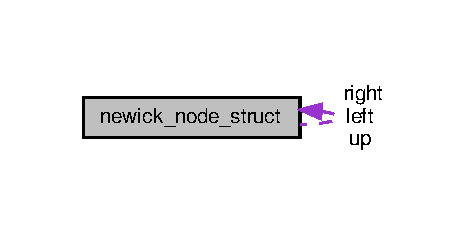
\includegraphics[width=224pt]{structnewick__node__struct__coll__graph}
\end{center}
\end{figure}
\subsubsection*{Data Fields}
\begin{DoxyCompactItemize}
\item 
\mbox{\Hypertarget{structnewick__node__struct_abf4311a6ecdcdb1e6d4392203296568c}\label{structnewick__node__struct_abf4311a6ecdcdb1e6d4392203296568c}} 
\hyperlink{structnewick__node__struct}{newick\+\_\+node} {\bfseries up}
\item 
\mbox{\Hypertarget{structnewick__node__struct_a928110516dfc1bec3703422f712cf076}\label{structnewick__node__struct_a928110516dfc1bec3703422f712cf076}} 
\hyperlink{structnewick__node__struct}{newick\+\_\+node} {\bfseries right}
\item 
\mbox{\Hypertarget{structnewick__node__struct_ae3b6eaf84d10df4685e241f6c535704c}\label{structnewick__node__struct_ae3b6eaf84d10df4685e241f6c535704c}} 
\hyperlink{structnewick__node__struct}{newick\+\_\+node} {\bfseries left}
\item 
\mbox{\Hypertarget{structnewick__node__struct_adf502c2f86d329cbb6531ae229fb6631}\label{structnewick__node__struct_adf502c2f86d329cbb6531ae229fb6631}} 
int \hyperlink{structnewick__node__struct_adf502c2f86d329cbb6531ae229fb6631}{id}
\begin{DoxyCompactList}\small\item\em Parent and children nodes. \end{DoxyCompactList}\item 
\mbox{\Hypertarget{structnewick__node__struct_a9205ab7cce347279634f90af83d1e81d}\label{structnewick__node__struct_a9205ab7cce347279634f90af83d1e81d}} 
double \hyperlink{structnewick__node__struct_a9205ab7cce347279634f90af83d1e81d}{branch\+\_\+length}
\begin{DoxyCompactList}\small\item\em Initial pre-\/order numbering of node. \end{DoxyCompactList}\item 
\mbox{\Hypertarget{structnewick__node__struct_a8d91f9fce7bf71a4c2723d64b402c868}\label{structnewick__node__struct_a8d91f9fce7bf71a4c2723d64b402c868}} 
char $\ast$ \hyperlink{structnewick__node__struct_a8d91f9fce7bf71a4c2723d64b402c868}{taxlabel}
\begin{DoxyCompactList}\small\item\em Branch length from node to node-\/$>$up. \end{DoxyCompactList}\end{DoxyCompactItemize}


\subsubsection{Detailed Description}
newick trees have minimal information, unlike \hyperlink{structtopology__struct}{topology\+\_\+struct} 

The documentation for this struct was generated from the following file\+:\begin{DoxyCompactItemize}
\item 
\hyperlink{read__newick__trees_8h}{read\+\_\+newick\+\_\+trees.\+h}\end{DoxyCompactItemize}

\hypertarget{structnewick__space__struct}{}\subsection{newick\+\_\+space\+\_\+struct Struct Reference}
\label{structnewick__space__struct}\index{newick\+\_\+space\+\_\+struct@{newick\+\_\+space\+\_\+struct}}


Collection of topologies from tree file. Each topology will have its own char\+\_\+vector.  




{\ttfamily \#include $<$newick\+\_\+space.\+h$>$}



Collaboration diagram for newick\+\_\+space\+\_\+struct\+:\nopagebreak
\begin{figure}[H]
\begin{center}
\leavevmode
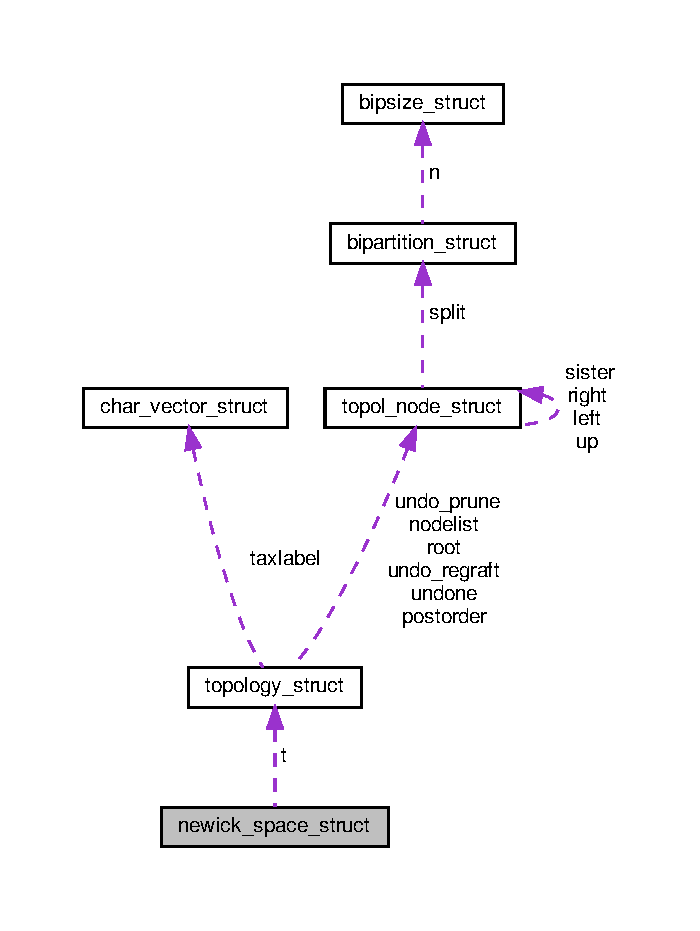
\includegraphics[width=336pt]{structnewick__space__struct__coll__graph}
\end{center}
\end{figure}
\subsubsection*{Data Fields}
\begin{DoxyCompactItemize}
\item 
\mbox{\Hypertarget{structnewick__space__struct_a9b7dd85f23e54a5aed85b5b1261673e8}\label{structnewick__space__struct_a9b7dd85f23e54a5aed85b5b1261673e8}} 
int {\bfseries ntrees}
\item 
\mbox{\Hypertarget{structnewick__space__struct_a08853acc734ac5d8da8f37d4f57cbe84}\label{structnewick__space__struct_a08853acc734ac5d8da8f37d4f57cbe84}} 
\hyperlink{structtopology__struct}{topology} $\ast$ \hyperlink{structnewick__space__struct_a08853acc734ac5d8da8f37d4f57cbe84}{t}
\begin{DoxyCompactList}\small\item\em Number of trees originally in nexus file and compacted (only distinct topologies). \end{DoxyCompactList}\item 
\mbox{\Hypertarget{structnewick__space__struct_ae4fdbf837e78c6116d54028686daf664}\label{structnewick__space__struct_ae4fdbf837e78c6116d54028686daf664}} 
int \hyperlink{structnewick__space__struct_ae4fdbf837e78c6116d54028686daf664}{ref\+\_\+counter}
\begin{DoxyCompactList}\small\item\em Vector of trees originally in nexus file and compacted. \end{DoxyCompactList}\end{DoxyCompactItemize}


\subsubsection{Detailed Description}
Collection of topologies from tree file. Each topology will have its own char\+\_\+vector. 

The documentation for this struct was generated from the following file\+:\begin{DoxyCompactItemize}
\item 
\hyperlink{newick__space_8h}{newick\+\_\+space.\+h}\end{DoxyCompactItemize}

\hypertarget{structnewick__tree__struct}{}\subsection{newick\+\_\+tree\+\_\+struct Struct Reference}
\label{structnewick__tree__struct}\index{newick\+\_\+tree\+\_\+struct@{newick\+\_\+tree\+\_\+struct}}


Collaboration diagram for newick\+\_\+tree\+\_\+struct\+:\nopagebreak
\begin{figure}[H]
\begin{center}
\leavevmode
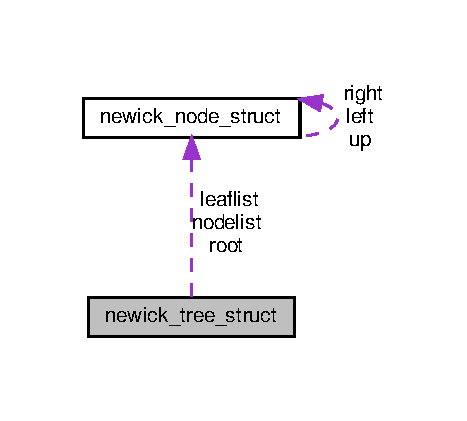
\includegraphics[width=224pt]{structnewick__tree__struct__coll__graph}
\end{center}
\end{figure}
\subsubsection*{Data Fields}
\begin{DoxyCompactItemize}
\item 
\mbox{\Hypertarget{structnewick__tree__struct_a20ac649fdca11eb6199683d5b5e0a323}\label{structnewick__tree__struct_a20ac649fdca11eb6199683d5b5e0a323}} 
\hyperlink{structnewick__node__struct}{newick\+\_\+node} $\ast$ {\bfseries nodelist}
\item 
\mbox{\Hypertarget{structnewick__tree__struct_a126b90aeb073ef366b41d315669224a9}\label{structnewick__tree__struct_a126b90aeb073ef366b41d315669224a9}} 
\hyperlink{structnewick__node__struct}{newick\+\_\+node} $\ast$ \hyperlink{structnewick__tree__struct_a126b90aeb073ef366b41d315669224a9}{leaflist}
\begin{DoxyCompactList}\small\item\em Vector with pointers to every internal node. \end{DoxyCompactList}\item 
\mbox{\Hypertarget{structnewick__tree__struct_a2225d85fcdecdb67bc87f15a4d3c6e6e}\label{structnewick__tree__struct_a2225d85fcdecdb67bc87f15a4d3c6e6e}} 
\hyperlink{structnewick__node__struct}{newick\+\_\+node} \hyperlink{structnewick__tree__struct_a2225d85fcdecdb67bc87f15a4d3c6e6e}{root}
\begin{DoxyCompactList}\small\item\em Vector with pointers to tree leaves. \end{DoxyCompactList}\item 
\mbox{\Hypertarget{structnewick__tree__struct_a1e1324fe64965530222840f6b77c5312}\label{structnewick__tree__struct_a1e1324fe64965530222840f6b77c5312}} 
int \hyperlink{structnewick__tree__struct_a1e1324fe64965530222840f6b77c5312}{nnodes}
\begin{DoxyCompactList}\small\item\em Pointer to root node. \end{DoxyCompactList}\item 
\mbox{\Hypertarget{structnewick__tree__struct_acfeb86d8e0c69b446a984ddd06999c19}\label{structnewick__tree__struct_acfeb86d8e0c69b446a984ddd06999c19}} 
int {\bfseries nleaves}
\end{DoxyCompactItemize}


The documentation for this struct was generated from the following file\+:\begin{DoxyCompactItemize}
\item 
\hyperlink{read__newick__trees_8h}{read\+\_\+newick\+\_\+trees.\+h}\end{DoxyCompactItemize}

\hypertarget{structpoint}{}\subsection{point Struct Reference}
\label{structpoint}\index{point@{point}}
\subsubsection*{Data Fields}
\begin{DoxyCompactItemize}
\item 
\mbox{\Hypertarget{structpoint_a5923982f66809b9bdde4d14fc7939259}\label{structpoint_a5923982f66809b9bdde4d14fc7939259}} 
int {\bfseries id}
\item 
\mbox{\Hypertarget{structpoint_ae2bc8ca43bce7bbe5520aa7aa1139f1d}\label{structpoint_ae2bc8ca43bce7bbe5520aa7aa1139f1d}} 
double {\bfseries core\+Dist}
\item 
\mbox{\Hypertarget{structpoint_a8d2201adcc02ecc543776c0a7befc06b}\label{structpoint_a8d2201adcc02ecc543776c0a7befc06b}} 
double {\bfseries reach\+Dist}
\item 
\mbox{\Hypertarget{structpoint_ae7ee439185943af4d6b9a0ead57ecc9a}\label{structpoint_ae7ee439185943af4d6b9a0ead57ecc9a}} 
\hyperlink{lowlevel_8h_a97a80ca1602ebf2303258971a2c938e2}{bool} {\bfseries processed}
\item 
\mbox{\Hypertarget{structpoint_a9d3ff9e10bcfd9c5f76ca5c9666cbea5}\label{structpoint_a9d3ff9e10bcfd9c5f76ca5c9666cbea5}} 
int {\bfseries pq\+Pos}
\end{DoxyCompactItemize}


The documentation for this struct was generated from the following file\+:\begin{DoxyCompactItemize}
\item 
clustering\+\_\+goptics.\+c\end{DoxyCompactItemize}

\hypertarget{structPriorityQueue}{}\subsection{Priority\+Queue Struct Reference}
\label{structPriorityQueue}\index{Priority\+Queue@{Priority\+Queue}}


Collaboration diagram for Priority\+Queue\+:\nopagebreak
\begin{figure}[H]
\begin{center}
\leavevmode
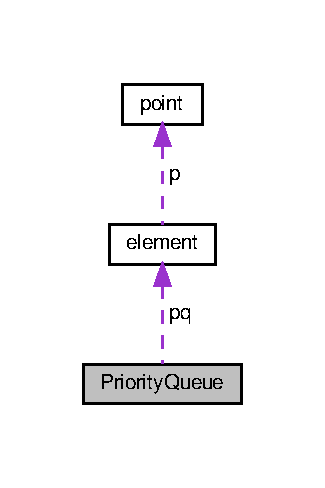
\includegraphics[width=156pt]{structPriorityQueue__coll__graph}
\end{center}
\end{figure}
\subsubsection*{Data Fields}
\begin{DoxyCompactItemize}
\item 
\mbox{\Hypertarget{structPriorityQueue_a9541f287cf1a4feaa9862f340d265c7a}\label{structPriorityQueue_a9541f287cf1a4feaa9862f340d265c7a}} 
\hyperlink{structelement}{element} $\ast$ {\bfseries pq}
\item 
\mbox{\Hypertarget{structPriorityQueue_ad3b9a7dbcd73abb046b17dc5647ad5a7}\label{structPriorityQueue_ad3b9a7dbcd73abb046b17dc5647ad5a7}} 
int {\bfseries n}
\item 
\mbox{\Hypertarget{structPriorityQueue_ac23c7a9940c29e1e6706c9ba26faaa35}\label{structPriorityQueue_ac23c7a9940c29e1e6706c9ba26faaa35}} 
int {\bfseries heap\+\_\+size}
\end{DoxyCompactItemize}


The documentation for this struct was generated from the following file\+:\begin{DoxyCompactItemize}
\item 
clustering\+\_\+goptics.\+c\end{DoxyCompactItemize}

\hypertarget{structprivhdr}{}\subsection{privhdr Struct Reference}
\label{structprivhdr}\index{privhdr@{privhdr}}
\subsubsection*{Data Fields}
\begin{DoxyCompactItemize}
\item 
\mbox{\Hypertarget{structprivhdr_af3739fb1871f5fed122dfcc86263b99f}\label{structprivhdr_af3739fb1871f5fed122dfcc86263b99f}} 
const char $\ast$ {\bfseries pattern}
\item 
\mbox{\Hypertarget{structprivhdr_af26cfd6c6c4e74efcb95e39dd2dc89da}\label{structprivhdr_af26cfd6c6c4e74efcb95e39dd2dc89da}} 
int {\bfseries flags}
\end{DoxyCompactItemize}


The documentation for this struct was generated from the following file\+:\begin{DoxyCompactItemize}
\item 
argtable3.\+c\end{DoxyCompactItemize}

\hypertarget{structreconciliation__struct}{}\subsection{reconciliation\+\_\+struct Struct Reference}
\label{structreconciliation__struct}\index{reconciliation\+\_\+struct@{reconciliation\+\_\+struct}}


mapping between gene tree nodes (this) and (external) species tree nodes  




{\ttfamily \#include $<$genetree.\+h$>$}



Collaboration diagram for reconciliation\+\_\+struct\+:\nopagebreak
\begin{figure}[H]
\begin{center}
\leavevmode
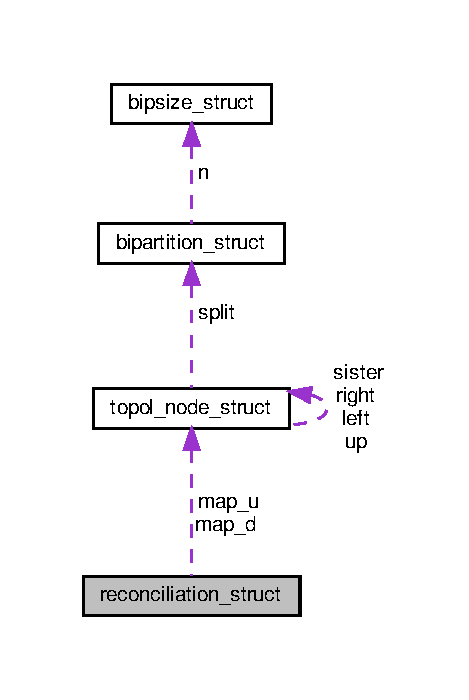
\includegraphics[width=225pt]{structreconciliation__struct__coll__graph}
\end{center}
\end{figure}
\subsubsection*{Data Fields}
\begin{DoxyCompactItemize}
\item 
\mbox{\Hypertarget{structreconciliation__struct_ac47989dd9997713d7024c27654fff1a9}\label{structreconciliation__struct_ac47989dd9997713d7024c27654fff1a9}} 
\hyperlink{structtopol__node__struct}{topol\+\_\+node} $\ast$ {\bfseries map\+\_\+d}
\item 
\mbox{\Hypertarget{structreconciliation__struct_af30cb9a5323cff3cf6c16e020c2ea6ae}\label{structreconciliation__struct_af30cb9a5323cff3cf6c16e020c2ea6ae}} 
\hyperlink{structtopol__node__struct}{topol\+\_\+node} $\ast$ \hyperlink{structreconciliation__struct_af30cb9a5323cff3cf6c16e020c2ea6ae}{map\+\_\+u}
\begin{DoxyCompactList}\small\item\em Mapping of all nodes from gene to species (the first gene\+::nnodes are fixed) \end{DoxyCompactList}\item 
\mbox{\Hypertarget{structreconciliation__struct_a58d7c66720179b77ae0aa54911d11c1f}\label{structreconciliation__struct_a58d7c66720179b77ae0aa54911d11c1f}} 
int $\ast$ \hyperlink{structreconciliation__struct_a58d7c66720179b77ae0aa54911d11c1f}{sp\+\_\+id}
\begin{DoxyCompactList}\small\item\em Mapping of all nodes from gene to species, assuming gene tree is upside down (unrooted T\+E\+S\+T\+I\+NG version) \end{DoxyCompactList}\item 
\mbox{\Hypertarget{structreconciliation__struct_a2b5f260452d8240e46afd2604b975e14}\label{structreconciliation__struct_a2b5f260452d8240e46afd2604b975e14}} 
int $\ast$ \hyperlink{structreconciliation__struct_a2b5f260452d8240e46afd2604b975e14}{sp\+\_\+count}
\begin{DoxyCompactList}\small\item\em mapping of gene (this tolopogy) leaf to ID of taxon in species tree \end{DoxyCompactList}\item 
\mbox{\Hypertarget{structreconciliation__struct_a89ac1a00c6c775cb5769396e832e58ef}\label{structreconciliation__struct_a89ac1a00c6c775cb5769396e832e58ef}} 
int \hyperlink{structreconciliation__struct_a89ac1a00c6c775cb5769396e832e58ef}{sp\+\_\+size}
\begin{DoxyCompactList}\small\item\em how many copies of each species are present in this gene (used by deepcoal) \end{DoxyCompactList}\item 
\mbox{\Hypertarget{structreconciliation__struct_aeb4f07f6c681cb938ecf5c8679555549}\label{structreconciliation__struct_aeb4f07f6c681cb938ecf5c8679555549}} 
int \hyperlink{structreconciliation__struct_aeb4f07f6c681cb938ecf5c8679555549}{size\+\_\+diff}
\begin{DoxyCompactList}\small\item\em effective number of species present in gene family \end{DoxyCompactList}\item 
\mbox{\Hypertarget{structreconciliation__struct_a407dc24ff413c06e6cf323f7e94916f1}\label{structreconciliation__struct_a407dc24ff413c06e6cf323f7e94916f1}} 
int $\ast$ \hyperlink{structreconciliation__struct_a407dc24ff413c06e6cf323f7e94916f1}{dup}
\begin{DoxyCompactList}\small\item\em twice the difference in number of leaves between gene tree and (reduced/effective) species tree \end{DoxyCompactList}\item 
\mbox{\Hypertarget{structreconciliation__struct_a9be3553faaa8bb74b66ce418eaaa736b}\label{structreconciliation__struct_a9be3553faaa8bb74b66ce418eaaa736b}} 
int $\ast$ \hyperlink{structreconciliation__struct_a9be3553faaa8bb74b66ce418eaaa736b}{ndup\+\_\+d}
\begin{DoxyCompactList}\small\item\em indexes of duplication nodes on gene tree, and number of such nodes (unused for now) \end{DoxyCompactList}\item 
\mbox{\Hypertarget{structreconciliation__struct_a69c92c622f67b5fd696cc0e0dca9ca9f}\label{structreconciliation__struct_a69c92c622f67b5fd696cc0e0dca9ca9f}} 
int $\ast$ \hyperlink{structreconciliation__struct_a69c92c622f67b5fd696cc0e0dca9ca9f}{ndup\+\_\+u}
\begin{DoxyCompactList}\small\item\em number of duplications below node (edge above node, since struct assume node == edge above it) \end{DoxyCompactList}\item 
\mbox{\Hypertarget{structreconciliation__struct_a26d88a04957a59b6c5223f4beb223a34}\label{structreconciliation__struct_a26d88a04957a59b6c5223f4beb223a34}} 
int $\ast$ \hyperlink{structreconciliation__struct_a26d88a04957a59b6c5223f4beb223a34}{nlos\+\_\+d}
\begin{DoxyCompactList}\small\item\em number of duplications above node (edge upside down, thus \char`\"{}children\char`\"{} are \textquotesingle{}up\textquotesingle{} and \textquotesingle{}sister\textquotesingle{}) \end{DoxyCompactList}\item 
\mbox{\Hypertarget{structreconciliation__struct_af78500445bc598675adbdda9afa2356a}\label{structreconciliation__struct_af78500445bc598675adbdda9afa2356a}} 
int $\ast$ \hyperlink{structreconciliation__struct_af78500445bc598675adbdda9afa2356a}{nlos\+\_\+u}
\begin{DoxyCompactList}\small\item\em number of losses below node and edge above node \end{DoxyCompactList}\item 
\mbox{\Hypertarget{structreconciliation__struct_a201c9966439f65c1bbf38eaf55cd0a3e}\label{structreconciliation__struct_a201c9966439f65c1bbf38eaf55cd0a3e}} 
int \hyperlink{structreconciliation__struct_a201c9966439f65c1bbf38eaf55cd0a3e}{ndups}
\begin{DoxyCompactList}\small\item\em number of losses above node, including edge above it \end{DoxyCompactList}\item 
\mbox{\Hypertarget{structreconciliation__struct_a9d66971cc3093b68a6145b174e07586a}\label{structreconciliation__struct_a9d66971cc3093b68a6145b174e07586a}} 
int \hyperlink{structreconciliation__struct_a9d66971cc3093b68a6145b174e07586a}{nloss}
\begin{DoxyCompactList}\small\item\em minimum number of duplications over all possible rootings, acc. to \hyperlink{structreconciliation__struct_a407dc24ff413c06e6cf323f7e94916f1}{reconciliation\+\_\+struct\+::dup} \end{DoxyCompactList}\item 
\mbox{\Hypertarget{structreconciliation__struct_ae0fbab68a1f81b74d8e8b35110924c91}\label{structreconciliation__struct_ae0fbab68a1f81b74d8e8b35110924c91}} 
int \hyperlink{structreconciliation__struct_ae0fbab68a1f81b74d8e8b35110924c91}{ndcos}
\begin{DoxyCompactList}\small\item\em number of losses corresponding to rooting (edge) that minimizes duplications \end{DoxyCompactList}\end{DoxyCompactItemize}


\subsubsection{Detailed Description}
mapping between gene tree nodes (this) and (external) species tree nodes 

The documentation for this struct was generated from the following file\+:\begin{DoxyCompactItemize}
\item 
\hyperlink{genetree_8h}{genetree.\+h}\end{DoxyCompactItemize}

\hypertarget{structrng__diaconis__struct}{}\subsection{rng\+\_\+diaconis\+\_\+struct Struct Reference}
\label{structrng__diaconis__struct}\index{rng\+\_\+diaconis\+\_\+struct@{rng\+\_\+diaconis\+\_\+struct}}


Persi Diaconis\textquotesingle{} lagged Fibonacci.  




{\ttfamily \#include $<$random\+\_\+number\+\_\+gen.\+h$>$}

\subsubsection*{Data Fields}
\begin{DoxyCompactItemize}
\item 
\mbox{\Hypertarget{structrng__diaconis__struct_a7dd3e9b29bc7b2bfad09c27c36dea94d}\label{structrng__diaconis__struct_a7dd3e9b29bc7b2bfad09c27c36dea94d}} 
uint32\+\_\+t {\bfseries x} \mbox{[}128\mbox{]}
\item 
\mbox{\Hypertarget{structrng__diaconis__struct_adb2691d0b3abf19d68365a660223ba68}\label{structrng__diaconis__struct_adb2691d0b3abf19d68365a660223ba68}} 
int {\bfseries n}
\end{DoxyCompactItemize}


\subsubsection{Detailed Description}
Persi Diaconis\textquotesingle{} lagged Fibonacci. 

The documentation for this struct was generated from the following file\+:\begin{DoxyCompactItemize}
\item 
random\+\_\+number\+\_\+gen.\+h\end{DoxyCompactItemize}

\hypertarget{structrng__gfsr4__struct}{}\subsection{rng\+\_\+gfsr4\+\_\+struct Struct Reference}
\label{structrng__gfsr4__struct}\index{rng\+\_\+gfsr4\+\_\+struct@{rng\+\_\+gfsr4\+\_\+struct}}


G\+F\+S\+R4 implementation from G\+SL.  




{\ttfamily \#include $<$random\+\_\+number\+\_\+gen.\+h$>$}

\subsubsection*{Data Fields}
\begin{DoxyCompactItemize}
\item 
\mbox{\Hypertarget{structrng__gfsr4__struct_a5622e035e156e3f0d1145dbefba83529}\label{structrng__gfsr4__struct_a5622e035e156e3f0d1145dbefba83529}} 
uint32\+\_\+t {\bfseries x} \mbox{[}16384\mbox{]}
\item 
\mbox{\Hypertarget{structrng__gfsr4__struct_ab5faf71596de1108c759669cf4345d37}\label{structrng__gfsr4__struct_ab5faf71596de1108c759669cf4345d37}} 
int {\bfseries n}
\end{DoxyCompactItemize}


\subsubsection{Detailed Description}
G\+F\+S\+R4 implementation from G\+SL. 

The documentation for this struct was generated from the following file\+:\begin{DoxyCompactItemize}
\item 
random\+\_\+number\+\_\+gen.\+h\end{DoxyCompactItemize}

\hypertarget{structrng__lfib4__struct}{}\subsection{rng\+\_\+lfib4\+\_\+struct Struct Reference}
\label{structrng__lfib4__struct}\index{rng\+\_\+lfib4\+\_\+struct@{rng\+\_\+lfib4\+\_\+struct}}


Marsaglia\textquotesingle{}s L\+F\+I\+B4 lagged Fibonacci using addition.  




{\ttfamily \#include $<$random\+\_\+number\+\_\+gen.\+h$>$}

\subsubsection*{Data Fields}
\begin{DoxyCompactItemize}
\item 
\mbox{\Hypertarget{structrng__lfib4__struct_a7fea3d3a8676a248a63b1f2640de79a5}\label{structrng__lfib4__struct_a7fea3d3a8676a248a63b1f2640de79a5}} 
uint32\+\_\+t {\bfseries x} \mbox{[}256\mbox{]}
\item 
\mbox{\Hypertarget{structrng__lfib4__struct_a00307570b79e5d3597091d2571834e62}\label{structrng__lfib4__struct_a00307570b79e5d3597091d2571834e62}} 
int {\bfseries n}
\end{DoxyCompactItemize}


\subsubsection{Detailed Description}
Marsaglia\textquotesingle{}s L\+F\+I\+B4 lagged Fibonacci using addition. 

The documentation for this struct was generated from the following file\+:\begin{DoxyCompactItemize}
\item 
random\+\_\+number\+\_\+gen.\+h\end{DoxyCompactItemize}

\hypertarget{structrng__mt19937__struct}{}\subsection{rng\+\_\+mt19937\+\_\+struct Struct Reference}
\label{structrng__mt19937__struct}\index{rng\+\_\+mt19937\+\_\+struct@{rng\+\_\+mt19937\+\_\+struct}}


M\+T19937-\/64, the Mersenne Twister for 64 bits.  




{\ttfamily \#include $<$random\+\_\+number\+\_\+gen.\+h$>$}

\subsubsection*{Data Fields}
\begin{DoxyCompactItemize}
\item 
\mbox{\Hypertarget{structrng__mt19937__struct_aa6645c0238b70abeae6ddf001106bd95}\label{structrng__mt19937__struct_aa6645c0238b70abeae6ddf001106bd95}} 
uint64\+\_\+t {\bfseries x} \mbox{[}312\mbox{]}
\item 
\mbox{\Hypertarget{structrng__mt19937__struct_a0bc4a64835d20417637939d75d298bd3}\label{structrng__mt19937__struct_a0bc4a64835d20417637939d75d298bd3}} 
int {\bfseries n}
\end{DoxyCompactItemize}


\subsubsection{Detailed Description}
M\+T19937-\/64, the Mersenne Twister for 64 bits. 

The documentation for this struct was generated from the following file\+:\begin{DoxyCompactItemize}
\item 
random\+\_\+number\+\_\+gen.\+h\end{DoxyCompactItemize}

\hypertarget{structrng__mt19937ar__struct}{}\subsection{rng\+\_\+mt19937ar\+\_\+struct Struct Reference}
\label{structrng__mt19937ar__struct}\index{rng\+\_\+mt19937ar\+\_\+struct@{rng\+\_\+mt19937ar\+\_\+struct}}


M\+T19937, the original Mersenne Twister (for 32 bits); the name \char`\"{}ar\char`\"{} comes from \char`\"{}array\char`\"{}.  




{\ttfamily \#include $<$random\+\_\+number\+\_\+gen.\+h$>$}

\subsubsection*{Data Fields}
\begin{DoxyCompactItemize}
\item 
\mbox{\Hypertarget{structrng__mt19937ar__struct_acab7bb9663018853f10184b9391a6537}\label{structrng__mt19937ar__struct_acab7bb9663018853f10184b9391a6537}} 
uint32\+\_\+t {\bfseries x} \mbox{[}624\mbox{]}
\item 
\mbox{\Hypertarget{structrng__mt19937ar__struct_a1fcbbb7a302db25bfc519f7f73e80c46}\label{structrng__mt19937ar__struct_a1fcbbb7a302db25bfc519f7f73e80c46}} 
int {\bfseries n}
\end{DoxyCompactItemize}


\subsubsection{Detailed Description}
M\+T19937, the original Mersenne Twister (for 32 bits); the name \char`\"{}ar\char`\"{} comes from \char`\"{}array\char`\"{}. 

The documentation for this struct was generated from the following file\+:\begin{DoxyCompactItemize}
\item 
random\+\_\+number\+\_\+gen.\+h\end{DoxyCompactItemize}

\hypertarget{structrng__swb__struct}{}\subsection{rng\+\_\+swb\+\_\+struct Struct Reference}
\label{structrng__swb__struct}\index{rng\+\_\+swb\+\_\+struct@{rng\+\_\+swb\+\_\+struct}}


Marsaglia\textquotesingle{}s Subtract-\/with-\/borrow generator.  




{\ttfamily \#include $<$random\+\_\+number\+\_\+gen.\+h$>$}

\subsubsection*{Data Fields}
\begin{DoxyCompactItemize}
\item 
\mbox{\Hypertarget{structrng__swb__struct_a234533129437be2de5fb9b6b45fba837}\label{structrng__swb__struct_a234533129437be2de5fb9b6b45fba837}} 
uint32\+\_\+t {\bfseries x} \mbox{[}258\mbox{]}
\item 
\mbox{\Hypertarget{structrng__swb__struct_a5e74e2b305ae34ff47e9f78e5802f75a}\label{structrng__swb__struct_a5e74e2b305ae34ff47e9f78e5802f75a}} 
int {\bfseries n}
\end{DoxyCompactItemize}


\subsubsection{Detailed Description}
Marsaglia\textquotesingle{}s Subtract-\/with-\/borrow generator. 

The documentation for this struct was generated from the following file\+:\begin{DoxyCompactItemize}
\item 
random\+\_\+number\+\_\+gen.\+h\end{DoxyCompactItemize}

\hypertarget{structrng__taus__struct}{}\subsection{rng\+\_\+taus\+\_\+struct Struct Reference}
\label{structrng__taus__struct}\index{rng\+\_\+taus\+\_\+struct@{rng\+\_\+taus\+\_\+struct}}
\subsubsection*{Data Fields}
\begin{DoxyCompactItemize}
\item 
\mbox{\Hypertarget{structrng__taus__struct_a24f685cd6bff45b43c137ff9f00baeea}\label{structrng__taus__struct_a24f685cd6bff45b43c137ff9f00baeea}} 
uint64\+\_\+t {\bfseries x} \mbox{[}30\mbox{]}
\item 
\mbox{\Hypertarget{structrng__taus__struct_a32c71f11d3efcf34680577387e8faf15}\label{structrng__taus__struct_a32c71f11d3efcf34680577387e8faf15}} 
int {\bfseries n}
\end{DoxyCompactItemize}


The documentation for this struct was generated from the following file\+:\begin{DoxyCompactItemize}
\item 
random\+\_\+number\+\_\+gen.\+h\end{DoxyCompactItemize}

\hypertarget{structrng__tt800__struct}{}\subsection{rng\+\_\+tt800\+\_\+struct Struct Reference}
\label{structrng__tt800__struct}\index{rng\+\_\+tt800\+\_\+struct@{rng\+\_\+tt800\+\_\+struct}}


tt800 (small cousin of M\+T19937, the Mersenne Twister)  




{\ttfamily \#include $<$random\+\_\+number\+\_\+gen.\+h$>$}

\subsubsection*{Data Fields}
\begin{DoxyCompactItemize}
\item 
\mbox{\Hypertarget{structrng__tt800__struct_ab9a57b75f7f6d7743f41c5d595a74e96}\label{structrng__tt800__struct_ab9a57b75f7f6d7743f41c5d595a74e96}} 
uint32\+\_\+t {\bfseries x} \mbox{[}25\mbox{]}
\item 
\mbox{\Hypertarget{structrng__tt800__struct_a3300fe5d7b6eae8bd0cb0edd86656860}\label{structrng__tt800__struct_a3300fe5d7b6eae8bd0cb0edd86656860}} 
int {\bfseries n}
\end{DoxyCompactItemize}


\subsubsection{Detailed Description}
tt800 (small cousin of M\+T19937, the Mersenne Twister) 

The documentation for this struct was generated from the following file\+:\begin{DoxyCompactItemize}
\item 
random\+\_\+number\+\_\+gen.\+h\end{DoxyCompactItemize}

\hypertarget{structrng__well1024__struct}{}\subsection{rng\+\_\+well1024\+\_\+struct Struct Reference}
\label{structrng__well1024__struct}\index{rng\+\_\+well1024\+\_\+struct@{rng\+\_\+well1024\+\_\+struct}}
\subsubsection*{Data Fields}
\begin{DoxyCompactItemize}
\item 
\mbox{\Hypertarget{structrng__well1024__struct_a8d407696371a130afedde3172b1c94ec}\label{structrng__well1024__struct_a8d407696371a130afedde3172b1c94ec}} 
uint32\+\_\+t {\bfseries x} \mbox{[}32\mbox{]}
\item 
\mbox{\Hypertarget{structrng__well1024__struct_a93b390b05add2c9f1eceda50b634b6da}\label{structrng__well1024__struct_a93b390b05add2c9f1eceda50b634b6da}} 
int {\bfseries n}
\end{DoxyCompactItemize}


The documentation for this struct was generated from the following file\+:\begin{DoxyCompactItemize}
\item 
random\+\_\+number\+\_\+gen.\+h\end{DoxyCompactItemize}

\hypertarget{structrng__xorshift__struct}{}\subsection{rng\+\_\+xorshift\+\_\+struct Struct Reference}
\label{structrng__xorshift__struct}\index{rng\+\_\+xorshift\+\_\+struct@{rng\+\_\+xorshift\+\_\+struct}}
\subsubsection*{Data Fields}
\begin{DoxyCompactItemize}
\item 
\mbox{\Hypertarget{structrng__xorshift__struct_ad6197a620f2c60cbe0c66534ea9247ee}\label{structrng__xorshift__struct_ad6197a620f2c60cbe0c66534ea9247ee}} 
uint64\+\_\+t {\bfseries x} \mbox{[}65\mbox{]}
\item 
\mbox{\Hypertarget{structrng__xorshift__struct_aca14bb6aaea04bbda0fe84a57ea632b4}\label{structrng__xorshift__struct_aca14bb6aaea04bbda0fe84a57ea632b4}} 
int {\bfseries n}
\end{DoxyCompactItemize}


The documentation for this struct was generated from the following file\+:\begin{DoxyCompactItemize}
\item 
random\+\_\+number\+\_\+gen.\+h\end{DoxyCompactItemize}

\hypertarget{structspdist__matrix__struct}{}\subsection{spdist\+\_\+matrix\+\_\+struct Struct Reference}
\label{structspdist__matrix__struct}\index{spdist\+\_\+matrix\+\_\+struct@{spdist\+\_\+matrix\+\_\+struct}}
\subsubsection*{Data Fields}
\begin{DoxyCompactItemize}
\item 
\mbox{\Hypertarget{structspdist__matrix__struct_ab3f9eb0ceaa1fe6638d657b937fd1257}\label{structspdist__matrix__struct_ab3f9eb0ceaa1fe6638d657b937fd1257}} 
int {\bfseries size}
\item 
\mbox{\Hypertarget{structspdist__matrix__struct_a44ae2df725c4fdb1da276d513878c573}\label{structspdist__matrix__struct_a44ae2df725c4fdb1da276d513878c573}} 
int {\bfseries n\+\_\+missing}
\item 
\mbox{\Hypertarget{structspdist__matrix__struct_a8841a7e54e32b1ef18e62ee60ffa60cb}\label{structspdist__matrix__struct_a8841a7e54e32b1ef18e62ee60ffa60cb}} 
double $\ast$ {\bfseries mean}
\item 
\mbox{\Hypertarget{structspdist__matrix__struct_a11ca683ad62f96fd4ec2ee10c875fc98}\label{structspdist__matrix__struct_a11ca683ad62f96fd4ec2ee10c875fc98}} 
double $\ast$ {\bfseries min}
\item 
\mbox{\Hypertarget{structspdist__matrix__struct_a4a537b8180ec0b33d4e263e03bd5d579}\label{structspdist__matrix__struct_a4a537b8180ec0b33d4e263e03bd5d579}} 
int $\ast$ \hyperlink{structspdist__matrix__struct_a4a537b8180ec0b33d4e263e03bd5d579}{count}
\begin{DoxyCompactList}\small\item\em mean or min distances across possibilities (within loci) \end{DoxyCompactList}\item 
\mbox{\Hypertarget{structspdist__matrix__struct_adf10eb5aea5957e231a5032c1f1c412e}\label{structspdist__matrix__struct_adf10eb5aea5957e231a5032c1f1c412e}} 
\hyperlink{lowlevel_8h_a97a80ca1602ebf2303258971a2c938e2}{bool} $\ast$ \hyperlink{structspdist__matrix__struct_adf10eb5aea5957e231a5032c1f1c412e}{species\+\_\+present}
\begin{DoxyCompactList}\small\item\em how many times this pairwise comparison appears (between or within loci) \end{DoxyCompactList}\item 
\mbox{\Hypertarget{structspdist__matrix__struct_a4c45767a5ee5888edfdb5ddb423fe5ca}\label{structspdist__matrix__struct_a4c45767a5ee5888edfdb5ddb423fe5ca}} 
int \hyperlink{structspdist__matrix__struct_a4c45767a5ee5888edfdb5ddb423fe5ca}{ref\+\_\+counter}
\begin{DoxyCompactList}\small\item\em boolean marking if species is present at all in this matrix \end{DoxyCompactList}\end{DoxyCompactItemize}


The documentation for this struct was generated from the following file\+:\begin{DoxyCompactItemize}
\item 
\hyperlink{distance__matrix_8h}{distance\+\_\+matrix.\+h}\end{DoxyCompactItemize}

\hypertarget{structspeciestree__struct}{}\subsection{speciestree\+\_\+struct Struct Reference}
\label{structspeciestree__struct}\index{speciestree\+\_\+struct@{speciestree\+\_\+struct}}


Collaboration diagram for speciestree\+\_\+struct\+:\nopagebreak
\begin{figure}[H]
\begin{center}
\leavevmode
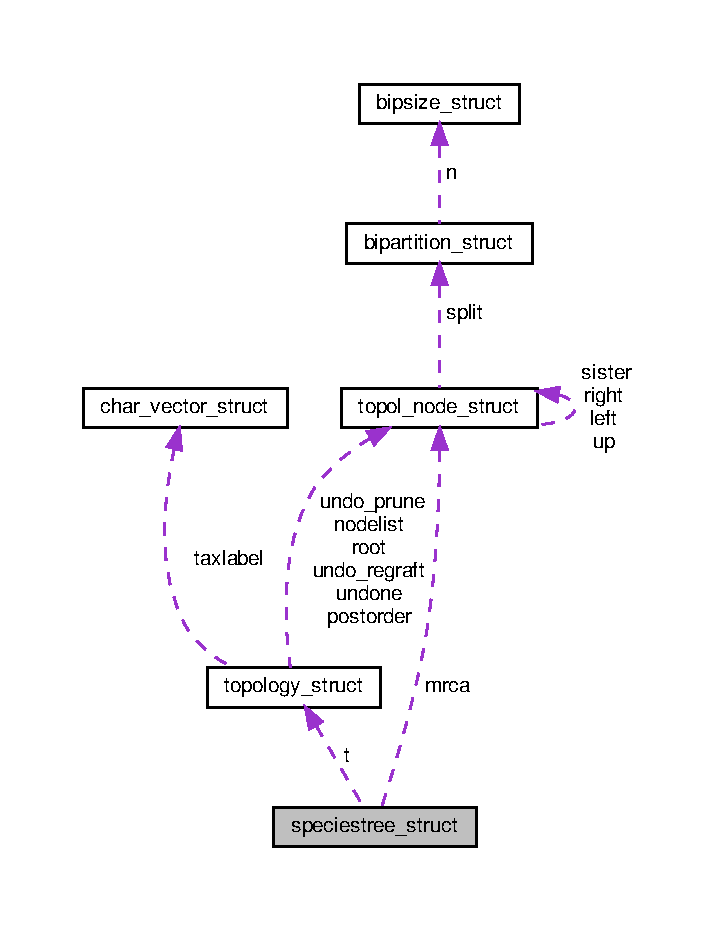
\includegraphics[width=344pt]{structspeciestree__struct__coll__graph}
\end{center}
\end{figure}
\subsubsection*{Data Fields}
\begin{DoxyCompactItemize}
\item 
\mbox{\Hypertarget{structspeciestree__struct_a55732a7f5b91645b88cb8b9a0d0d0b7c}\label{structspeciestree__struct_a55732a7f5b91645b88cb8b9a0d0d0b7c}} 
\hyperlink{structtopology__struct}{topology} {\bfseries t}
\item 
\mbox{\Hypertarget{structspeciestree__struct_a88e2a63f6df55342314b5f7d898e54f8}\label{structspeciestree__struct_a88e2a63f6df55342314b5f7d898e54f8}} 
\hyperlink{structtopol__node__struct}{topol\+\_\+node} $\ast$ {\bfseries mrca}
\item 
\mbox{\Hypertarget{structspeciestree__struct_a70069c66ad4062e05d0b6a6641866729}\label{structspeciestree__struct_a70069c66ad4062e05d0b6a6641866729}} 
int $\ast$ \hyperlink{structspeciestree__struct_a70069c66ad4062e05d0b6a6641866729}{spnames\+\_\+order}
\begin{DoxyCompactList}\small\item\em triangular matrix of topol\+\_\+nodes (L\+CA between \hyperlink{structtopol__node__struct_aa59aaa71c57b79b7737eb72973485a0a}{topol\+\_\+node\+::id} (i-\/1) and j) in one dimension \end{DoxyCompactList}\item 
\mbox{\Hypertarget{structspeciestree__struct_af043a320e1bab001712b1fc59a1fa950}\label{structspeciestree__struct_af043a320e1bab001712b1fc59a1fa950}} 
int \hyperlink{structspeciestree__struct_af043a320e1bab001712b1fc59a1fa950}{ref\+\_\+counter}
\begin{DoxyCompactList}\small\item\em Length+lexico order of sptree leaf names (not used unless added by user, when arbitrary leaf ordering is requested) \end{DoxyCompactList}\end{DoxyCompactItemize}


The documentation for this struct was generated from the following file\+:\begin{DoxyCompactItemize}
\item 
\hyperlink{genetree_8h}{genetree.\+h}\end{DoxyCompactItemize}

\hypertarget{structsplitset__struct}{}\subsection{splitset\+\_\+struct Struct Reference}
\label{structsplitset__struct}\index{splitset\+\_\+struct@{splitset\+\_\+struct}}


Collaboration diagram for splitset\+\_\+struct\+:\nopagebreak
\begin{figure}[H]
\begin{center}
\leavevmode
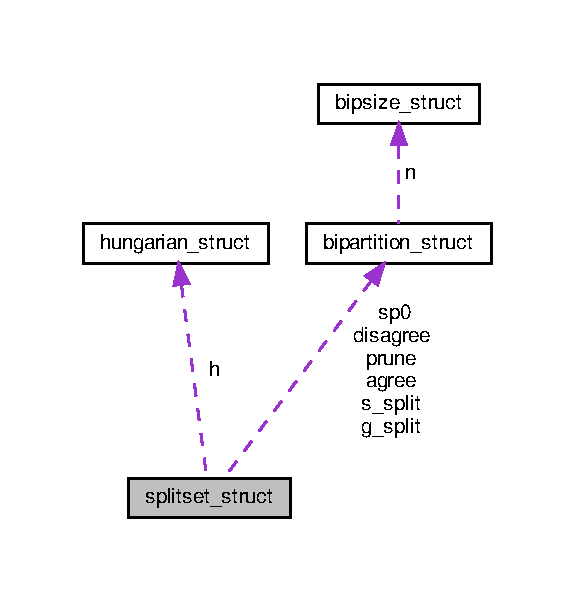
\includegraphics[width=276pt]{structsplitset__struct__coll__graph}
\end{center}
\end{figure}
\subsubsection*{Data Fields}
\begin{DoxyCompactItemize}
\item 
\mbox{\Hypertarget{structsplitset__struct_af0d4564c44bcaff08461fe7bec1bbe13}\label{structsplitset__struct_af0d4564c44bcaff08461fe7bec1bbe13}} 
int {\bfseries size}
\item 
\mbox{\Hypertarget{structsplitset__struct_a2b389f9524f0c01831ebd72f60a05939}\label{structsplitset__struct_a2b389f9524f0c01831ebd72f60a05939}} 
int {\bfseries spsize}
\item 
\mbox{\Hypertarget{structsplitset__struct_afaff8951790761f96cb3da25c3493790}\label{structsplitset__struct_afaff8951790761f96cb3da25c3493790}} 
int {\bfseries spr}
\item 
\mbox{\Hypertarget{structsplitset__struct_aa6b2ef3d64746cf55e830f9e43d06ed9}\label{structsplitset__struct_aa6b2ef3d64746cf55e830f9e43d06ed9}} 
int {\bfseries spr\+\_\+extra}
\item 
\mbox{\Hypertarget{structsplitset__struct_a10f8784951d4a3adc62e1666a5caeebb}\label{structsplitset__struct_a10f8784951d4a3adc62e1666a5caeebb}} 
int {\bfseries rf}
\item 
\mbox{\Hypertarget{structsplitset__struct_a39b0070a47fbf625a3d1b5cbbf36f113}\label{structsplitset__struct_a39b0070a47fbf625a3d1b5cbbf36f113}} 
int {\bfseries hdist}
\item 
\mbox{\Hypertarget{structsplitset__struct_a30caa7dd87e5e99aec92b2fd48cb71f4}\label{structsplitset__struct_a30caa7dd87e5e99aec92b2fd48cb71f4}} 
int {\bfseries hdist\+\_\+reduced}
\item 
\mbox{\Hypertarget{structsplitset__struct_af7ba4428e2049a8f8c50215fc8c9e3b5}\label{structsplitset__struct_af7ba4428e2049a8f8c50215fc8c9e3b5}} 
int \hyperlink{structsplitset__struct_af7ba4428e2049a8f8c50215fc8c9e3b5}{n\+\_\+g}
\begin{DoxyCompactList}\small\item\em spr, extra prunes for spr, rf distances and hdist=assignment cost \end{DoxyCompactList}\item 
\mbox{\Hypertarget{structsplitset__struct_a7b08d1b651b28e889650095b180bfd16}\label{structsplitset__struct_a7b08d1b651b28e889650095b180bfd16}} 
int {\bfseries n\+\_\+s}
\item 
\mbox{\Hypertarget{structsplitset__struct_ada9ed313c4a36897b613f54cf9870d10}\label{structsplitset__struct_ada9ed313c4a36897b613f54cf9870d10}} 
int {\bfseries n\+\_\+agree}
\item 
\mbox{\Hypertarget{structsplitset__struct_a1b9ae7e54568a077701202c155e9a452}\label{structsplitset__struct_a1b9ae7e54568a077701202c155e9a452}} 
int {\bfseries n\+\_\+disagree}
\item 
\mbox{\Hypertarget{structsplitset__struct_aaa363e10399b35c959fb098997fa1ec0}\label{structsplitset__struct_aaa363e10399b35c959fb098997fa1ec0}} 
\hyperlink{structbipartition__struct}{bipartition} $\ast$ {\bfseries g\+\_\+split}
\item 
\mbox{\Hypertarget{structsplitset__struct_ac4f82828f0f20dfe186cb7a9f4175ce2}\label{structsplitset__struct_ac4f82828f0f20dfe186cb7a9f4175ce2}} 
\hyperlink{structbipartition__struct}{bipartition} $\ast$ {\bfseries s\+\_\+split}
\item 
\mbox{\Hypertarget{structsplitset__struct_a52c156ca7ddc538c82abeedf6d597b3c}\label{structsplitset__struct_a52c156ca7ddc538c82abeedf6d597b3c}} 
\hyperlink{structbipartition__struct}{bipartition} $\ast$ {\bfseries agree}
\item 
\mbox{\Hypertarget{structsplitset__struct_afc33a4395225755f920f141e39c7a7dc}\label{structsplitset__struct_afc33a4395225755f920f141e39c7a7dc}} 
\hyperlink{structbipartition__struct}{bipartition} $\ast$ {\bfseries disagree}
\item 
\mbox{\Hypertarget{structsplitset__struct_a56330277abfeeef40fe27b09c4dfaab9}\label{structsplitset__struct_a56330277abfeeef40fe27b09c4dfaab9}} 
\hyperlink{structbipartition__struct}{bipartition} $\ast$ {\bfseries sp0}
\item 
\mbox{\Hypertarget{structsplitset__struct_a635414eb91fc1c5588135c3d2e6285a1}\label{structsplitset__struct_a635414eb91fc1c5588135c3d2e6285a1}} 
\hyperlink{structbipartition__struct}{bipartition} {\bfseries prune}
\item 
\mbox{\Hypertarget{structsplitset__struct_a4d1c7adbbcfb9d3e78d8d895ac5988b4}\label{structsplitset__struct_a4d1c7adbbcfb9d3e78d8d895ac5988b4}} 
\hyperlink{structhungarian__struct}{hungarian} {\bfseries h}
\item 
\mbox{\Hypertarget{structsplitset__struct_aef440d73c8ff17adad125b6b61261464}\label{structsplitset__struct_aef440d73c8ff17adad125b6b61261464}} 
\hyperlink{lowlevel_8h_a97a80ca1602ebf2303258971a2c938e2}{bool} {\bfseries match}
\end{DoxyCompactItemize}


The documentation for this struct was generated from the following file\+:\begin{DoxyCompactItemize}
\item 
\hyperlink{genetree_8h}{genetree.\+h}\end{DoxyCompactItemize}

\hypertarget{structtagTRexNode}{}\subsection{tag\+T\+Rex\+Node Struct Reference}
\label{structtagTRexNode}\index{tag\+T\+Rex\+Node@{tag\+T\+Rex\+Node}}
\subsubsection*{Data Fields}
\begin{DoxyCompactItemize}
\item 
\mbox{\Hypertarget{structtagTRexNode_a24e6220291da90346d9a0780cfad7c7f}\label{structtagTRexNode_a24e6220291da90346d9a0780cfad7c7f}} 
T\+Rex\+Node\+Type {\bfseries type}
\item 
\mbox{\Hypertarget{structtagTRexNode_a4d1d697c3c82b29a41e6b4be0640da92}\label{structtagTRexNode_a4d1d697c3c82b29a41e6b4be0640da92}} 
int {\bfseries left}
\item 
\mbox{\Hypertarget{structtagTRexNode_a95eb4fe058e12dc38fd7126f2956633a}\label{structtagTRexNode_a95eb4fe058e12dc38fd7126f2956633a}} 
int {\bfseries right}
\item 
\mbox{\Hypertarget{structtagTRexNode_a9722e37dadf65b6fac9d8d9ce942b060}\label{structtagTRexNode_a9722e37dadf65b6fac9d8d9ce942b060}} 
int {\bfseries next}
\end{DoxyCompactItemize}


The documentation for this struct was generated from the following file\+:\begin{DoxyCompactItemize}
\item 
argtable3.\+c\end{DoxyCompactItemize}

\hypertarget{structtopol__node__struct}{}\subsection{topol\+\_\+node\+\_\+struct Struct Reference}
\label{structtopol__node__struct}\index{topol\+\_\+node\+\_\+struct@{topol\+\_\+node\+\_\+struct}}


Information of a node (binary tree).  




{\ttfamily \#include $<$topology\+\_\+common.\+h$>$}



Collaboration diagram for topol\+\_\+node\+\_\+struct\+:\nopagebreak
\begin{figure}[H]
\begin{center}
\leavevmode
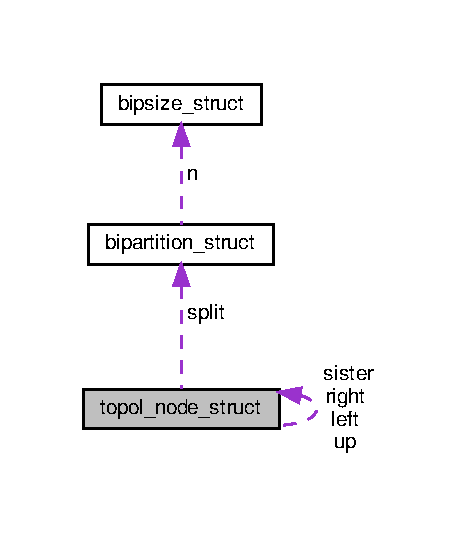
\includegraphics[width=220pt]{structtopol__node__struct__coll__graph}
\end{center}
\end{figure}
\subsubsection*{Data Fields}
\begin{DoxyCompactItemize}
\item 
\mbox{\Hypertarget{structtopol__node__struct_a747d302eeeec71b6c656e097e3a1658b}\label{structtopol__node__struct_a747d302eeeec71b6c656e097e3a1658b}} 
\hyperlink{structtopol__node__struct}{topol\+\_\+node} {\bfseries up}
\item 
\mbox{\Hypertarget{structtopol__node__struct_a0f2d377e06066861d52e5a55c4a057a5}\label{structtopol__node__struct_a0f2d377e06066861d52e5a55c4a057a5}} 
\hyperlink{structtopol__node__struct}{topol\+\_\+node} {\bfseries right}
\item 
\mbox{\Hypertarget{structtopol__node__struct_ac89c082b65b84e5822126f95552e9aa4}\label{structtopol__node__struct_ac89c082b65b84e5822126f95552e9aa4}} 
\hyperlink{structtopol__node__struct}{topol\+\_\+node} {\bfseries left}
\item 
\mbox{\Hypertarget{structtopol__node__struct_a2c32701d91360029c423c9a3d166eabf}\label{structtopol__node__struct_a2c32701d91360029c423c9a3d166eabf}} 
\hyperlink{structtopol__node__struct}{topol\+\_\+node} {\bfseries sister}
\item 
\mbox{\Hypertarget{structtopol__node__struct_aa59aaa71c57b79b7737eb72973485a0a}\label{structtopol__node__struct_aa59aaa71c57b79b7737eb72973485a0a}} 
int \hyperlink{structtopol__node__struct_aa59aaa71c57b79b7737eb72973485a0a}{id}
\begin{DoxyCompactList}\small\item\em Parent, children and sister nodes. \end{DoxyCompactList}\item 
\mbox{\Hypertarget{structtopol__node__struct_a0163a947756838115a3da8590fd88e46}\label{structtopol__node__struct_a0163a947756838115a3da8590fd88e46}} 
int {\bfseries level}
\item 
\mbox{\Hypertarget{structtopol__node__struct_a11adf7521b107205fafb609d23c75d52}\label{structtopol__node__struct_a11adf7521b107205fafb609d23c75d52}} 
int \hyperlink{structtopol__node__struct_a11adf7521b107205fafb609d23c75d52}{mid} \mbox{[}5\mbox{]}
\begin{DoxyCompactList}\small\item\em Node ID (values smaller than nleaves indicate leaves) and distance from root. \end{DoxyCompactList}\item 
\mbox{\Hypertarget{structtopol__node__struct_a0d9191d12975f8876bf490ab1ae9285b}\label{structtopol__node__struct_a0d9191d12975f8876bf490ab1ae9285b}} 
\hyperlink{lowlevel_8h_a97a80ca1602ebf2303258971a2c938e2}{bool} \hyperlink{structtopol__node__struct_a0d9191d12975f8876bf490ab1ae9285b}{internal}
\begin{DoxyCompactList}\small\item\em Mapping between nodes and postorder vectors \mbox{[}0,1\mbox{]} (postorder, undone); idx for deep coal \mbox{[}2,3\mbox{]} and losses \mbox{[}4\mbox{]}. \end{DoxyCompactList}\item 
\mbox{\Hypertarget{structtopol__node__struct_abb2445a6e496485e310620d4cb23fc3f}\label{structtopol__node__struct_abb2445a6e496485e310620d4cb23fc3f}} 
\hyperlink{lowlevel_8h_a97a80ca1602ebf2303258971a2c938e2}{bool} \hyperlink{structtopol__node__struct_abb2445a6e496485e310620d4cb23fc3f}{u\+\_\+done}
\begin{DoxyCompactList}\small\item\em If internal node, T\+R\+UE; if leaf, F\+A\+L\+SE. \end{DoxyCompactList}\item 
\mbox{\Hypertarget{structtopol__node__struct_a8a18b8003f8534d99a5b9936b652c8a4}\label{structtopol__node__struct_a8a18b8003f8534d99a5b9936b652c8a4}} 
\hyperlink{lowlevel_8h_a97a80ca1602ebf2303258971a2c938e2}{bool} \hyperlink{structtopol__node__struct_a8a18b8003f8534d99a5b9936b652c8a4}{d\+\_\+done}
\begin{DoxyCompactList}\small\item\em Has the topology up this edge (eq. to node) changed? (needed in likelihood calc) \end{DoxyCompactList}\item 
\mbox{\Hypertarget{structtopol__node__struct_aab1db55910dcf5f4e8b3d451aa0a8422}\label{structtopol__node__struct_aab1db55910dcf5f4e8b3d451aa0a8422}} 
\hyperlink{structbipartition__struct}{bipartition} \hyperlink{structtopol__node__struct_aab1db55910dcf5f4e8b3d451aa0a8422}{split}
\begin{DoxyCompactList}\small\item\em Has the topology down this edge (eq. to node) changed? (needed in likelihood calc) \end{DoxyCompactList}\end{DoxyCompactItemize}


\subsubsection{Detailed Description}
Information of a node (binary tree). 

The documentation for this struct was generated from the following file\+:\begin{DoxyCompactItemize}
\item 
\hyperlink{topology__common_8h}{topology\+\_\+common.\+h}\end{DoxyCompactItemize}

\hypertarget{structtopology__space__struct}{}\subsection{topology\+\_\+space\+\_\+struct Struct Reference}
\label{structtopology__space__struct}\index{topology\+\_\+space\+\_\+struct@{topology\+\_\+space\+\_\+struct}}


Collection of topologies from tree file. When topologies have no branch lengths we store only unique topologies.  




{\ttfamily \#include $<$topology\+\_\+space.\+h$>$}



Collaboration diagram for topology\+\_\+space\+\_\+struct\+:\nopagebreak
\begin{figure}[H]
\begin{center}
\leavevmode
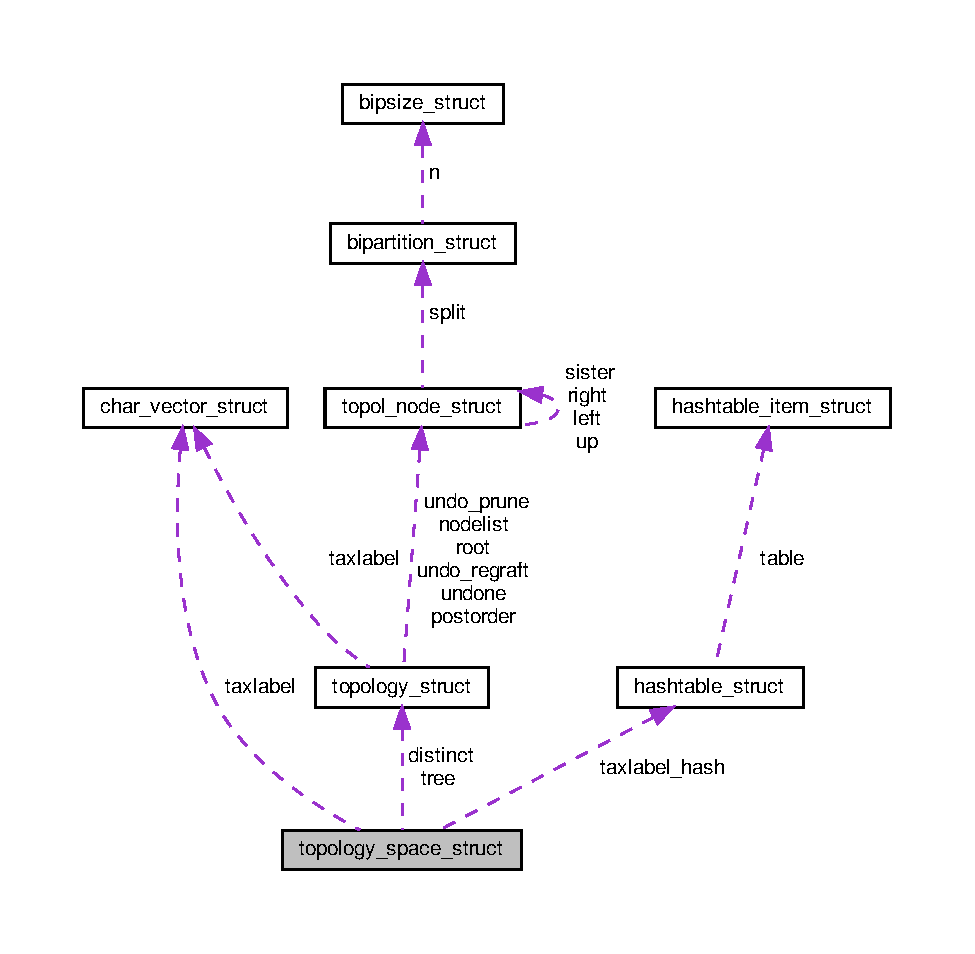
\includegraphics[width=350pt]{structtopology__space__struct__coll__graph}
\end{center}
\end{figure}
\subsubsection*{Data Fields}
\begin{DoxyCompactItemize}
\item 
\mbox{\Hypertarget{structtopology__space__struct_ab0a9425ca296b9cd5f471e1c6e628820}\label{structtopology__space__struct_ab0a9425ca296b9cd5f471e1c6e628820}} 
int {\bfseries ntrees}
\item 
\mbox{\Hypertarget{structtopology__space__struct_a9b52b128de956bc31a338ec74c5bf92d}\label{structtopology__space__struct_a9b52b128de956bc31a338ec74c5bf92d}} 
int {\bfseries ndistinct}
\item 
\mbox{\Hypertarget{structtopology__space__struct_a812703670e22b57734a453e09f5d9fe3}\label{structtopology__space__struct_a812703670e22b57734a453e09f5d9fe3}} 
\hyperlink{structtopology__struct}{topology} $\ast$ \hyperlink{structtopology__space__struct_a812703670e22b57734a453e09f5d9fe3}{tree}
\begin{DoxyCompactList}\small\item\em Number of trees originally in nexus file and compacted (only distinct topologies). \end{DoxyCompactList}\item 
\mbox{\Hypertarget{structtopology__space__struct_a04a02a86583f3ca577ec52b133a1f4b3}\label{structtopology__space__struct_a04a02a86583f3ca577ec52b133a1f4b3}} 
\hyperlink{structtopology__struct}{topology} $\ast$ {\bfseries distinct}
\item 
\mbox{\Hypertarget{structtopology__space__struct_a1b1c1f92bce9530c3f1ea363a5f03135}\label{structtopology__space__struct_a1b1c1f92bce9530c3f1ea363a5f03135}} 
double $\ast$ \hyperlink{structtopology__space__struct_a1b1c1f92bce9530c3f1ea363a5f03135}{freq}
\begin{DoxyCompactList}\small\item\em Vector of trees originally in nexus file and compacted. \end{DoxyCompactList}\item 
\mbox{\Hypertarget{structtopology__space__struct_ac1b12d8b3461a8e28cdbc40b5ae8ebaa}\label{structtopology__space__struct_ac1b12d8b3461a8e28cdbc40b5ae8ebaa}} 
\hyperlink{structchar__vector__struct}{char\+\_\+vector} \hyperlink{structtopology__space__struct_ac1b12d8b3461a8e28cdbc40b5ae8ebaa}{taxlabel}
\begin{DoxyCompactList}\small\item\em frequency of each distinct topology (add up to one) \end{DoxyCompactList}\item 
\mbox{\Hypertarget{structtopology__space__struct_ae8c62b1c65eedf80b1df6cea3e35ca7b}\label{structtopology__space__struct_ae8c62b1c65eedf80b1df6cea3e35ca7b}} 
\hyperlink{structhashtable__struct}{hashtable} \hyperlink{structtopology__space__struct_ae8c62b1c65eedf80b1df6cea3e35ca7b}{taxlabel\+\_\+hash}
\begin{DoxyCompactList}\small\item\em Taxon names. \end{DoxyCompactList}\item 
\mbox{\Hypertarget{structtopology__space__struct_a593fcc350fe442e1c4e8c7cec3474acd}\label{structtopology__space__struct_a593fcc350fe442e1c4e8c7cec3474acd}} 
\hyperlink{lowlevel_8h_a97a80ca1602ebf2303258971a2c938e2}{bool} \hyperlink{structtopology__space__struct_a593fcc350fe442e1c4e8c7cec3474acd}{is\+\_\+rooted}
\begin{DoxyCompactList}\small\item\em Lookup table with taxon names. \end{DoxyCompactList}\item 
\mbox{\Hypertarget{structtopology__space__struct_a711d7574fc7468e6c8098c08b1391e57}\label{structtopology__space__struct_a711d7574fc7468e6c8098c08b1391e57}} 
char $\ast$ \hyperlink{structtopology__space__struct_a711d7574fc7468e6c8098c08b1391e57}{filename}
\begin{DoxyCompactList}\small\item\em If trees are unrooted, then branch lengths must be accounted for in some comparisons. \end{DoxyCompactList}\end{DoxyCompactItemize}


\subsubsection{Detailed Description}
Collection of topologies from tree file. When topologies have no branch lengths we store only unique topologies. 

The documentation for this struct was generated from the following file\+:\begin{DoxyCompactItemize}
\item 
\hyperlink{topology__space_8h}{topology\+\_\+space.\+h}\end{DoxyCompactItemize}

\hypertarget{structtopology__struct}{}\subsection{topology\+\_\+struct Struct Reference}
\label{structtopology__struct}\index{topology\+\_\+struct@{topology\+\_\+struct}}


Binary unrooted topology (rooted at leaf with ID zero)  




{\ttfamily \#include $<$topology\+\_\+common.\+h$>$}



Collaboration diagram for topology\+\_\+struct\+:\nopagebreak
\begin{figure}[H]
\begin{center}
\leavevmode
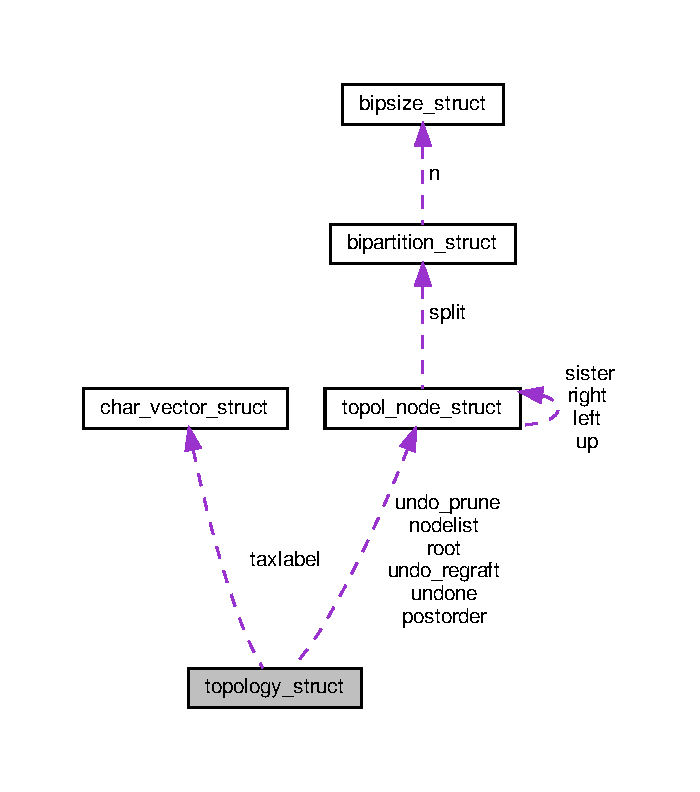
\includegraphics[width=336pt]{structtopology__struct__coll__graph}
\end{center}
\end{figure}
\subsubsection*{Data Fields}
\begin{DoxyCompactItemize}
\item 
\mbox{\Hypertarget{structtopology__struct_a352f502c9d84b575472264872ffb15f9}\label{structtopology__struct_a352f502c9d84b575472264872ffb15f9}} 
\hyperlink{structtopol__node__struct}{topol\+\_\+node} $\ast$ {\bfseries nodelist}
\item 
\mbox{\Hypertarget{structtopology__struct_acff9f1279985bba8c925f23e3e1b402f}\label{structtopology__struct_acff9f1279985bba8c925f23e3e1b402f}} 
double $\ast$ \hyperlink{structtopology__struct_acff9f1279985bba8c925f23e3e1b402f}{blength}
\begin{DoxyCompactList}\small\item\em vector of nodes (the first $L$ are the leaves). \end{DoxyCompactList}\item 
\mbox{\Hypertarget{structtopology__struct_a4e06620b64c11507e0970dce07de138e}\label{structtopology__struct_a4e06620b64c11507e0970dce07de138e}} 
int \hyperlink{structtopology__struct_a4e06620b64c11507e0970dce07de138e}{id}
\begin{DoxyCompactList}\small\item\em Branch lengths, with mean, min, max vectors for topology\+\_\+space. \end{DoxyCompactList}\item 
\mbox{\Hypertarget{structtopology__struct_a1b636052614bfd03729f580bed52c429}\label{structtopology__struct_a1b636052614bfd03729f580bed52c429}} 
\hyperlink{structtopol__node__struct}{topol\+\_\+node} \hyperlink{structtopology__struct_a1b636052614bfd03729f580bed52c429}{root}
\begin{DoxyCompactList}\small\item\em topology ID (should be updated by hand, e.\+g. by functions in topology\+\_\+space.\+c) \end{DoxyCompactList}\item 
\mbox{\Hypertarget{structtopology__struct_a792c38326b5188ea14cf166b7013f05b}\label{structtopology__struct_a792c38326b5188ea14cf166b7013f05b}} 
int \hyperlink{structtopology__struct_a792c38326b5188ea14cf166b7013f05b}{nleaves}
\begin{DoxyCompactList}\small\item\em Pointer to root node. \end{DoxyCompactList}\item 
\mbox{\Hypertarget{structtopology__struct_a7eab86ca5fc4e2c0df67b39065eaed95}\label{structtopology__struct_a7eab86ca5fc4e2c0df67b39065eaed95}} 
int \hyperlink{structtopology__struct_a7eab86ca5fc4e2c0df67b39065eaed95}{nnodes}
\begin{DoxyCompactList}\small\item\em Number of leaves $L$. \end{DoxyCompactList}\item 
\mbox{\Hypertarget{structtopology__struct_ade334ca8a90127e831eb67326bf159f5}\label{structtopology__struct_ade334ca8a90127e831eb67326bf159f5}} 
\hyperlink{structtopol__node__struct}{topol\+\_\+node} \hyperlink{structtopology__struct_ade334ca8a90127e831eb67326bf159f5}{undo\+\_\+prune}
\begin{DoxyCompactList}\small\item\em Number of nodes, including leaves ( $ 2L-1$ for a binary rooted tree). \end{DoxyCompactList}\item 
\mbox{\Hypertarget{structtopology__struct_a935865d3894e0918dbf7e9b6d74ee74d}\label{structtopology__struct_a935865d3894e0918dbf7e9b6d74ee74d}} 
\hyperlink{structtopol__node__struct}{topol\+\_\+node} \hyperlink{structtopology__struct_a935865d3894e0918dbf7e9b6d74ee74d}{undo\+\_\+regraft}
\begin{DoxyCompactList}\small\item\em How to revert most recent S\+PR move (prune node). \end{DoxyCompactList}\item 
\mbox{\Hypertarget{structtopology__struct_a69d8ce96ed99816f3cff56af36c9b44e}\label{structtopology__struct_a69d8ce96ed99816f3cff56af36c9b44e}} 
\hyperlink{lowlevel_8h_a97a80ca1602ebf2303258971a2c938e2}{bool} \hyperlink{structtopology__struct_a69d8ce96ed99816f3cff56af36c9b44e}{undo\+\_\+lca}
\begin{DoxyCompactList}\small\item\em How to revert most recent S\+PR move (regraft node). \end{DoxyCompactList}\item 
\mbox{\Hypertarget{structtopology__struct_a4a4ec9adb1812fa74c50b1355ed43711}\label{structtopology__struct_a4a4ec9adb1812fa74c50b1355ed43711}} 
\hyperlink{structtopol__node__struct}{topol\+\_\+node} $\ast$ \hyperlink{structtopology__struct_a4a4ec9adb1812fa74c50b1355ed43711}{postorder}
\begin{DoxyCompactList}\small\item\em revert S\+PR move is lca type or not \end{DoxyCompactList}\item 
\mbox{\Hypertarget{structtopology__struct_af2564b454d8c1c3a92f91d116a40cb9f}\label{structtopology__struct_af2564b454d8c1c3a92f91d116a40cb9f}} 
\hyperlink{structtopol__node__struct}{topol\+\_\+node} $\ast$ \hyperlink{structtopology__struct_af2564b454d8c1c3a92f91d116a40cb9f}{undone}
\begin{DoxyCompactList}\small\item\em pointers to all internal nodes in postorder (from last to first is preorder) \end{DoxyCompactList}\item 
\mbox{\Hypertarget{structtopology__struct_a9b8d78548796d309bedaccabce5ef3e2}\label{structtopology__struct_a9b8d78548796d309bedaccabce5ef3e2}} 
int \hyperlink{structtopology__struct_a9b8d78548796d309bedaccabce5ef3e2}{n\+\_\+undone}
\begin{DoxyCompactList}\small\item\em pointers to outdated nodes in postorder (from last to first is preorder) \end{DoxyCompactList}\item 
\mbox{\Hypertarget{structtopology__struct_a3755c32316ecb1418cd5403ac49bfc8a}\label{structtopology__struct_a3755c32316ecb1418cd5403ac49bfc8a}} 
uint32\+\_\+t \hyperlink{structtopology__struct_a3755c32316ecb1418cd5403ac49bfc8a}{hash\+I\+D1}
\begin{DoxyCompactList}\small\item\em number of outdated nodes (which need likelihood calc etc) in \hyperlink{structtopology__struct_af2564b454d8c1c3a92f91d116a40cb9f}{topology\+\_\+struct\+::undone}. \end{DoxyCompactList}\item 
\mbox{\Hypertarget{structtopology__struct_a075093f506de0dbe33c4f4385d429d46}\label{structtopology__struct_a075093f506de0dbe33c4f4385d429d46}} 
uint32\+\_\+t {\bfseries hash\+I\+D2}
\item 
\mbox{\Hypertarget{structtopology__struct_ac0951ef0fe8bb99631fef979d11c93c7}\label{structtopology__struct_ac0951ef0fe8bb99631fef979d11c93c7}} 
\hyperlink{lowlevel_8h_a97a80ca1602ebf2303258971a2c938e2}{bool} \hyperlink{structtopology__struct_ac0951ef0fe8bb99631fef979d11c93c7}{traversal\+\_\+updated}
\begin{DoxyCompactList}\small\item\em hash values of tree, ideally a unique value for each tree (collisions happen...) \end{DoxyCompactList}\item 
\mbox{\Hypertarget{structtopology__struct_af34229c1a7f6312c4ca98c05b12aacc2}\label{structtopology__struct_af34229c1a7f6312c4ca98c05b12aacc2}} 
int \hyperlink{structtopology__struct_af34229c1a7f6312c4ca98c05b12aacc2}{ref\+\_\+counter}
\begin{DoxyCompactList}\small\item\em zero if postorder\mbox{[}\mbox{]} vector needs update, one if we can use postdorder\mbox{[}\mbox{]} to traverse tree \end{DoxyCompactList}\item 
\mbox{\Hypertarget{structtopology__struct_a5b607230aba25816247ff1a6de879364}\label{structtopology__struct_a5b607230aba25816247ff1a6de879364}} 
\hyperlink{structchar__vector__struct}{char\+\_\+vector} \hyperlink{structtopology__struct_a5b607230aba25816247ff1a6de879364}{taxlabel}
\begin{DoxyCompactList}\small\item\em number of references of topology (how many places are pointing to it) \end{DoxyCompactList}\item 
\mbox{\Hypertarget{structtopology__struct_aaa2d082ac0e89064cfef0295cad42192}\label{structtopology__struct_aaa2d082ac0e89064cfef0295cad42192}} 
int $\ast$ \hyperlink{structtopology__struct_aaa2d082ac0e89064cfef0295cad42192}{index}
\begin{DoxyCompactList}\small\item\em Taxon names (just a pointer; actual values are setup by \hyperlink{structnewick__tree__struct}{newick\+\_\+tree\+\_\+struct} or \hyperlink{structalignment__struct}{alignment\+\_\+struct}) \end{DoxyCompactList}\item 
\mbox{\Hypertarget{structtopology__struct_a9ef01e28228f17731ab9fdb9ea98cb4f}\label{structtopology__struct_a9ef01e28228f17731ab9fdb9ea98cb4f}} 
\hyperlink{lowlevel_8h_a97a80ca1602ebf2303258971a2c938e2}{bool} \hyperlink{structtopology__struct_a9ef01e28228f17731ab9fdb9ea98cb4f}{quasirandom}
\begin{DoxyCompactList}\small\item\em sandbox vector used in spr moves / quasirandom tree shuffle just to avoid recurrent allocation \end{DoxyCompactList}\end{DoxyCompactItemize}


\subsubsection{Detailed Description}
Binary unrooted topology (rooted at leaf with ID zero) 

The documentation for this struct was generated from the following file\+:\begin{DoxyCompactItemize}
\item 
\hyperlink{topology__common_8h}{topology\+\_\+common.\+h}\end{DoxyCompactItemize}

\hypertarget{structTRex}{}\subsection{T\+Rex Struct Reference}
\label{structTRex}\index{T\+Rex@{T\+Rex}}


Collaboration diagram for T\+Rex\+:\nopagebreak
\begin{figure}[H]
\begin{center}
\leavevmode
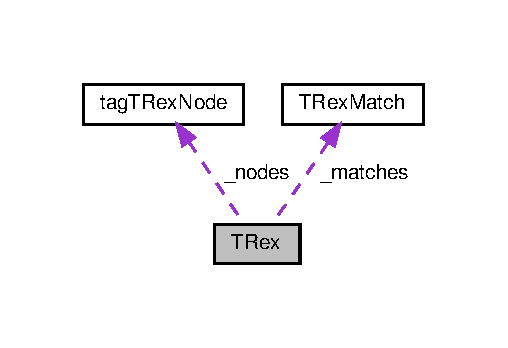
\includegraphics[width=244pt]{structTRex__coll__graph}
\end{center}
\end{figure}
\subsubsection*{Data Fields}
\begin{DoxyCompactItemize}
\item 
\mbox{\Hypertarget{structTRex_a274f6c4c42ea88341f3a3d8fbe51bf77}\label{structTRex_a274f6c4c42ea88341f3a3d8fbe51bf77}} 
const T\+Rex\+Char $\ast$ {\bfseries \+\_\+eol}
\item 
\mbox{\Hypertarget{structTRex_a728080945e8627daa0c4700b7fb031bb}\label{structTRex_a728080945e8627daa0c4700b7fb031bb}} 
const T\+Rex\+Char $\ast$ {\bfseries \+\_\+bol}
\item 
\mbox{\Hypertarget{structTRex_a177d1cad0312711ecd950e2d1e988247}\label{structTRex_a177d1cad0312711ecd950e2d1e988247}} 
const T\+Rex\+Char $\ast$ {\bfseries \+\_\+p}
\item 
\mbox{\Hypertarget{structTRex_aacc5ca371e83bcf649594cf12740901b}\label{structTRex_aacc5ca371e83bcf649594cf12740901b}} 
int {\bfseries \+\_\+first}
\item 
\mbox{\Hypertarget{structTRex_aec22a5029c705af4d3dde30763beeeb0}\label{structTRex_aec22a5029c705af4d3dde30763beeeb0}} 
int {\bfseries \+\_\+op}
\item 
\mbox{\Hypertarget{structTRex_aa7fc6649cbdb2c0f06de57bbe8c1c4a3}\label{structTRex_aa7fc6649cbdb2c0f06de57bbe8c1c4a3}} 
\hyperlink{structtagTRexNode}{T\+Rex\+Node} $\ast$ {\bfseries \+\_\+nodes}
\item 
\mbox{\Hypertarget{structTRex_af92121dc1268e3a33c615e94459aab16}\label{structTRex_af92121dc1268e3a33c615e94459aab16}} 
int {\bfseries \+\_\+nallocated}
\item 
\mbox{\Hypertarget{structTRex_a0f06b4807bd70a663a648ab29d6266c6}\label{structTRex_a0f06b4807bd70a663a648ab29d6266c6}} 
int {\bfseries \+\_\+nsize}
\item 
\mbox{\Hypertarget{structTRex_ab7a28e510b4fdeb7920e6828765a12e0}\label{structTRex_ab7a28e510b4fdeb7920e6828765a12e0}} 
int {\bfseries \+\_\+nsubexpr}
\item 
\mbox{\Hypertarget{structTRex_a4d6b9a4107f01bf17e39140269a91294}\label{structTRex_a4d6b9a4107f01bf17e39140269a91294}} 
\hyperlink{structTRexMatch}{T\+Rex\+Match} $\ast$ {\bfseries \+\_\+matches}
\item 
\mbox{\Hypertarget{structTRex_ae7439ae9edb7f5e469962b8b32a6dc25}\label{structTRex_ae7439ae9edb7f5e469962b8b32a6dc25}} 
int {\bfseries \+\_\+currsubexp}
\item 
\mbox{\Hypertarget{structTRex_a7f65f110bbc4437a1793b6ac125bdaae}\label{structTRex_a7f65f110bbc4437a1793b6ac125bdaae}} 
void $\ast$ {\bfseries \+\_\+jmpbuf}
\item 
\mbox{\Hypertarget{structTRex_a2b7c3784b3088fdeee20f074f757800c}\label{structTRex_a2b7c3784b3088fdeee20f074f757800c}} 
const T\+Rex\+Char $\ast$$\ast$ {\bfseries \+\_\+error}
\item 
\mbox{\Hypertarget{structTRex_aefdff38a9ed9d544fe4a92fed3163981}\label{structTRex_aefdff38a9ed9d544fe4a92fed3163981}} 
int {\bfseries \+\_\+flags}
\end{DoxyCompactItemize}


The documentation for this struct was generated from the following file\+:\begin{DoxyCompactItemize}
\item 
argtable3.\+c\end{DoxyCompactItemize}

\hypertarget{structTRexMatch}{}\subsection{T\+Rex\+Match Struct Reference}
\label{structTRexMatch}\index{T\+Rex\+Match@{T\+Rex\+Match}}
\subsubsection*{Data Fields}
\begin{DoxyCompactItemize}
\item 
\mbox{\Hypertarget{structTRexMatch_ac855b7327c66c06de72b44f13f3710d4}\label{structTRexMatch_ac855b7327c66c06de72b44f13f3710d4}} 
const T\+Rex\+Char $\ast$ {\bfseries begin}
\item 
\mbox{\Hypertarget{structTRexMatch_a35c1748bcb4d876e2ef5385a14641c2a}\label{structTRexMatch_a35c1748bcb4d876e2ef5385a14641c2a}} 
int {\bfseries len}
\end{DoxyCompactItemize}


The documentation for this struct was generated from the following file\+:\begin{DoxyCompactItemize}
\item 
argtable3.\+c\end{DoxyCompactItemize}

\section{File Documentation}
\hypertarget{alignment_8h}{}\subsection{alignment.\+h File Reference}
\label{alignment_8h}\index{alignment.\+h@{alignment.\+h}}


File handling functions and calculation of distances for sequence data in nexus format.  


{\ttfamily \#include \char`\"{}distance\+\_\+matrix.\+h\char`\"{}}\newline
{\ttfamily \#include \char`\"{}nexus\+\_\+common.\+h\char`\"{}}\newline
Include dependency graph for alignment.\+h\+:\nopagebreak
\begin{figure}[H]
\begin{center}
\leavevmode
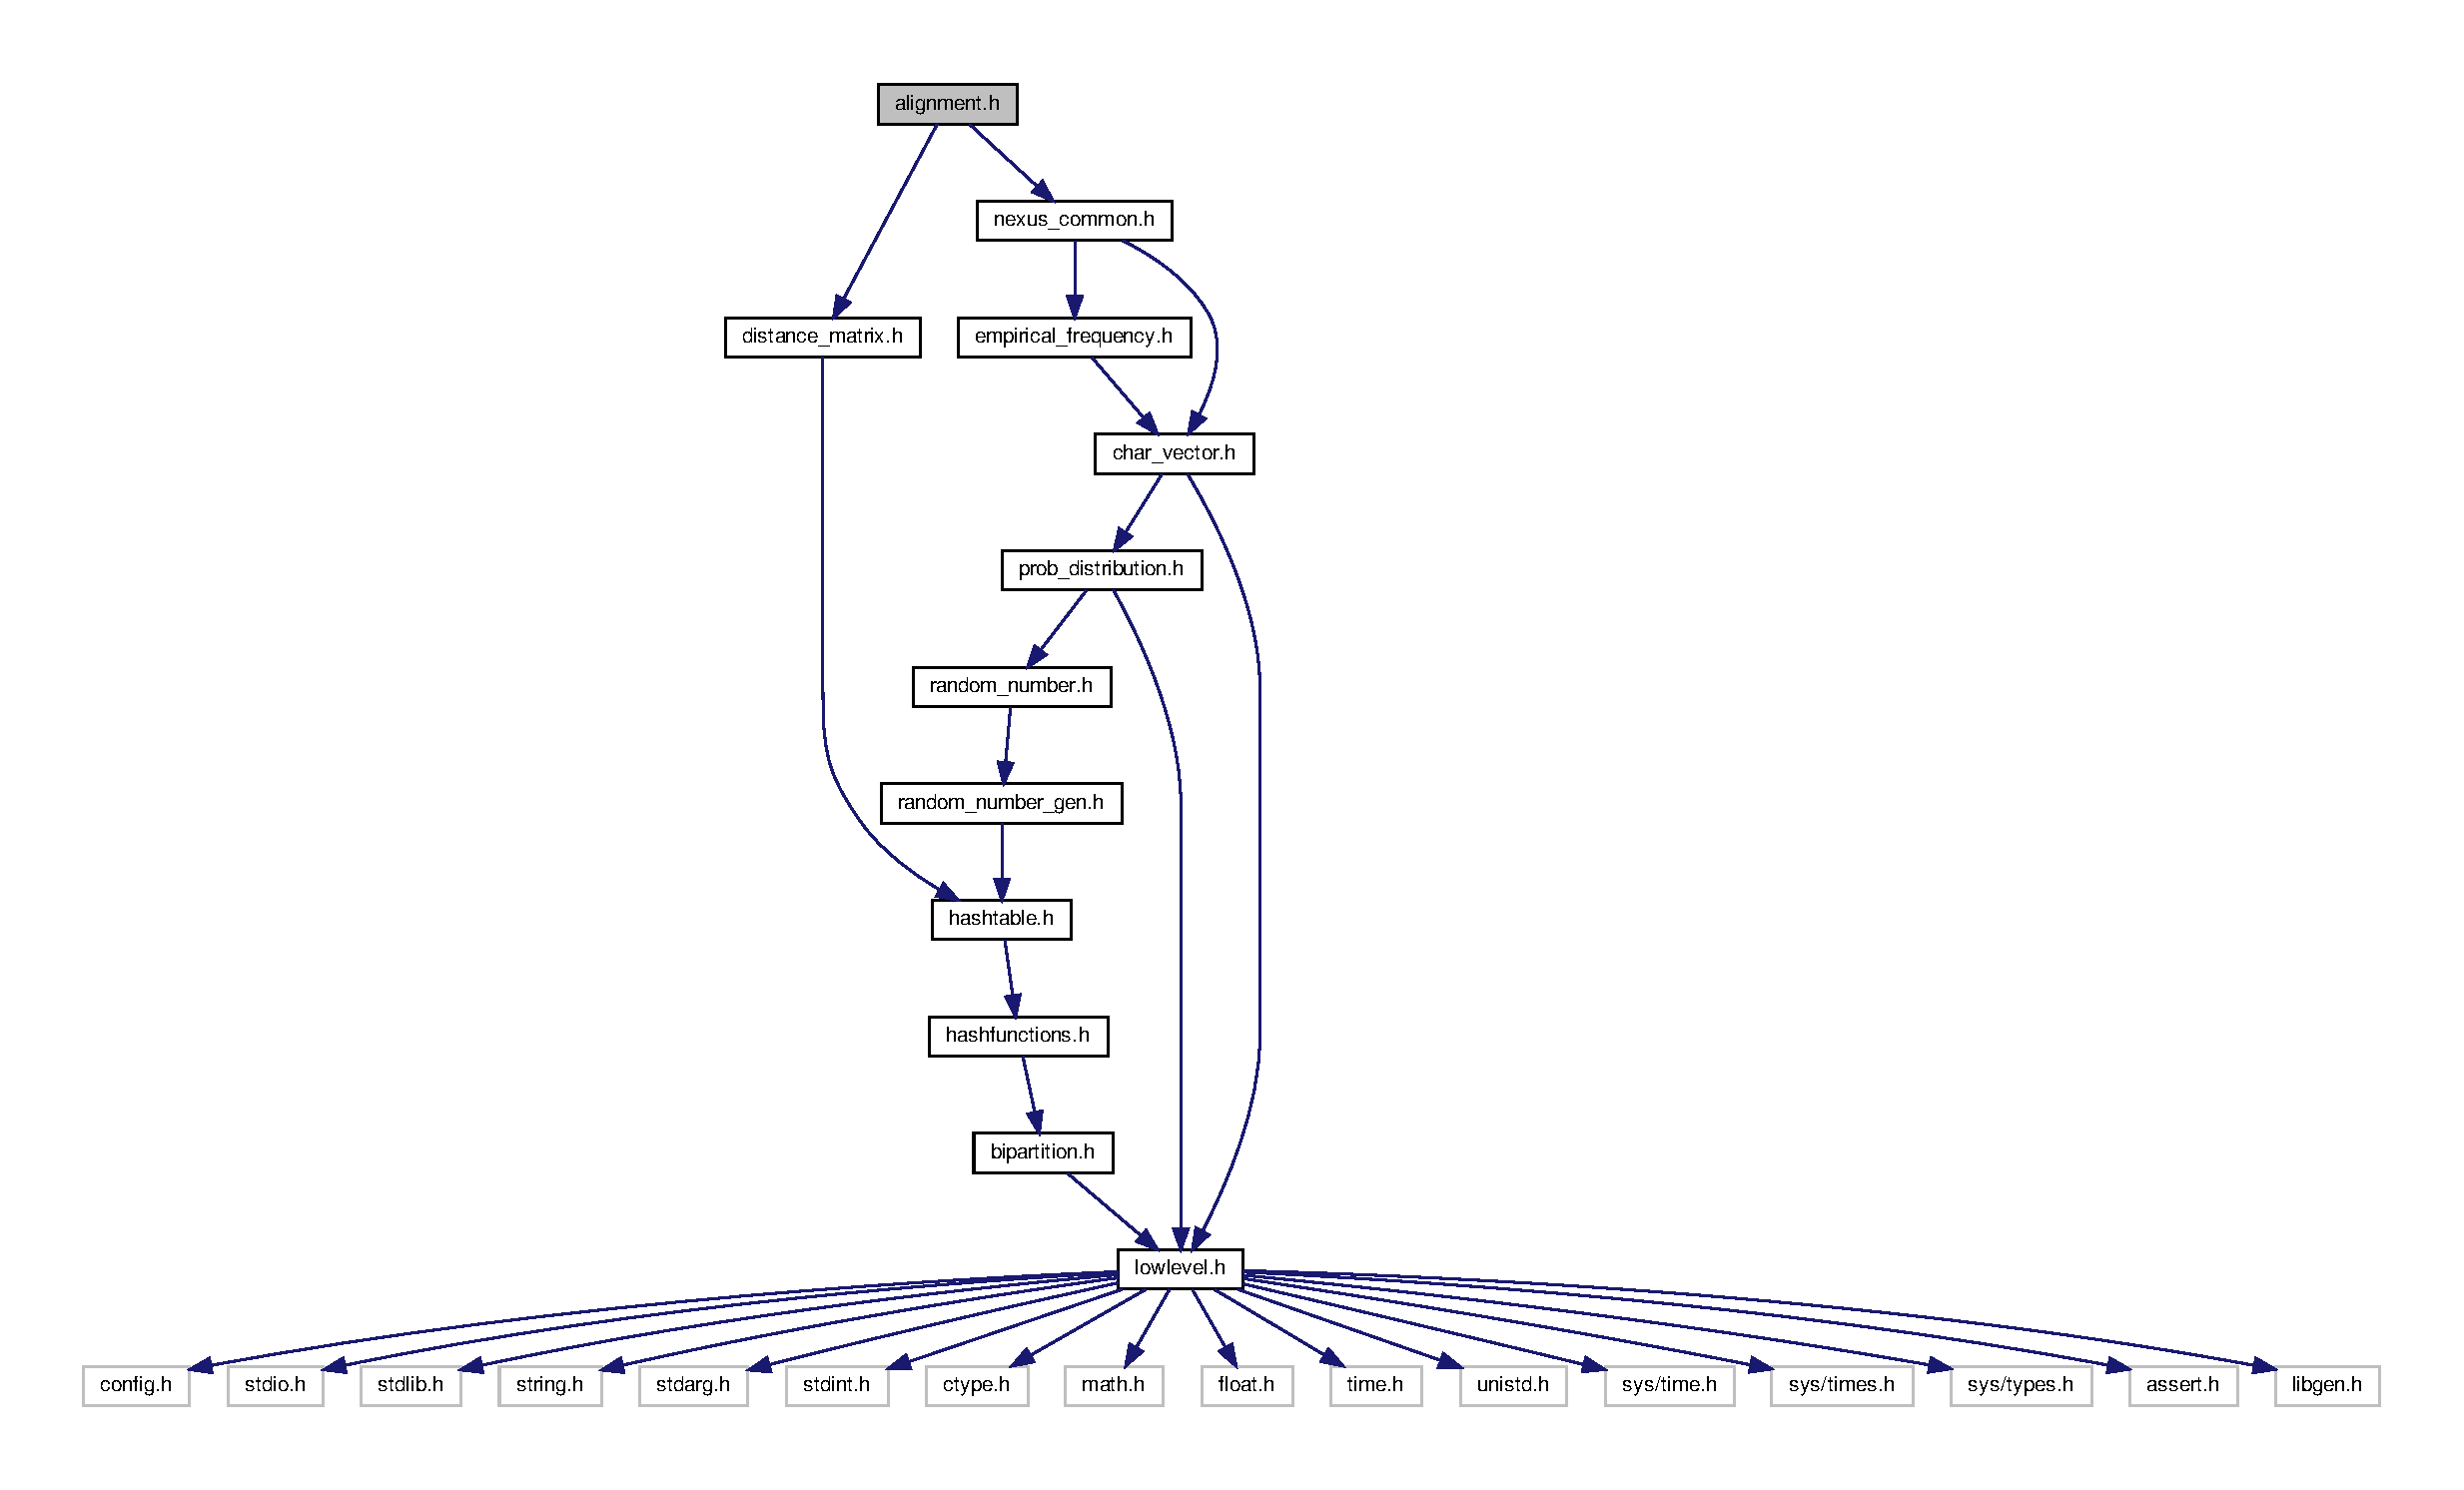
\includegraphics[width=350pt]{alignment_8h__incl}
\end{center}
\end{figure}
This graph shows which files directly or indirectly include this file\+:\nopagebreak
\begin{figure}[H]
\begin{center}
\leavevmode
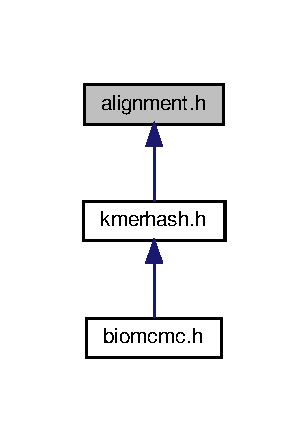
\includegraphics[width=148pt]{alignment_8h__dep__incl}
\end{center}
\end{figure}
\subsubsection*{Data Structures}
\begin{DoxyCompactItemize}
\item 
struct \hyperlink{structalignment__struct}{alignment\+\_\+struct}
\begin{DoxyCompactList}\small\item\em Data from alignment file. \end{DoxyCompactList}\end{DoxyCompactItemize}
\subsubsection*{Typedefs}
\begin{DoxyCompactItemize}
\item 
\mbox{\Hypertarget{alignment_8h_ab92d2b81028457d293c6e56b2c2b815c}\label{alignment_8h_ab92d2b81028457d293c6e56b2c2b815c}} 
typedef struct \hyperlink{structalignment__struct}{alignment\+\_\+struct} $\ast$ {\bfseries alignment}
\end{DoxyCompactItemize}
\subsubsection*{Functions}
\begin{DoxyCompactItemize}
\item 
\mbox{\Hypertarget{alignment_8h_aa036d9585db0e7f896efff4e37ffd5cb}\label{alignment_8h_aa036d9585db0e7f896efff4e37ffd5cb}} 
\hyperlink{structalignment__struct}{alignment} \hyperlink{alignment_8h_aa036d9585db0e7f896efff4e37ffd5cb}{read\+\_\+alignment\+\_\+from\+\_\+file} (char $\ast$seqfilename)
\begin{DoxyCompactList}\small\item\em Reads D\+NA alignment (guess format between F\+A\+S\+TA and N\+E\+X\+US) from file and store info in \hyperlink{structalignment__struct}{alignment\+\_\+struct}. \end{DoxyCompactList}\item 
\mbox{\Hypertarget{alignment_8h_a57980b340fee11061ad4511efc7b7c47}\label{alignment_8h_a57980b340fee11061ad4511efc7b7c47}} 
\hyperlink{structalignment__struct}{alignment} \hyperlink{alignment_8h_a57980b340fee11061ad4511efc7b7c47}{read\+\_\+fasta\+\_\+alignment\+\_\+from\+\_\+file} (char $\ast$seqfilename)
\begin{DoxyCompactList}\small\item\em Reads D\+NA F\+A\+S\+TA alignment from file and store info in \hyperlink{structalignment__struct}{alignment\+\_\+struct}. \end{DoxyCompactList}\item 
\mbox{\Hypertarget{alignment_8h_a5bd5335c2fd2fcf8c30e1becfea64b2c}\label{alignment_8h_a5bd5335c2fd2fcf8c30e1becfea64b2c}} 
\hyperlink{structalignment__struct}{alignment} \hyperlink{alignment_8h_a5bd5335c2fd2fcf8c30e1becfea64b2c}{read\+\_\+nexus\+\_\+alignment\+\_\+from\+\_\+file} (char $\ast$seqfilename)
\begin{DoxyCompactList}\small\item\em Reads D\+NA N\+E\+X\+US alignment from file and store info in \hyperlink{structalignment__struct}{alignment\+\_\+struct}. \end{DoxyCompactList}\item 
\mbox{\Hypertarget{alignment_8h_ae7be6382b75167950cff01c19dbbe166}\label{alignment_8h_ae7be6382b75167950cff01c19dbbe166}} 
void \hyperlink{alignment_8h_ae7be6382b75167950cff01c19dbbe166}{print\+\_\+alignment\+\_\+in\+\_\+fasta\+\_\+format} (\hyperlink{structalignment__struct}{alignment} align, F\+I\+LE $\ast$stream)
\begin{DoxyCompactList}\small\item\em Prints alignment to F\+I\+LE stream in F\+A\+S\+TA format (debug purposes). \end{DoxyCompactList}\item 
\mbox{\Hypertarget{alignment_8h_a98e39e61ac259230b72c60d7f033bdd4}\label{alignment_8h_a98e39e61ac259230b72c60d7f033bdd4}} 
void \hyperlink{alignment_8h_a98e39e61ac259230b72c60d7f033bdd4}{del\+\_\+alignment} (\hyperlink{structalignment__struct}{alignment} align)
\begin{DoxyCompactList}\small\item\em Frees memory from \hyperlink{structalignment__struct}{alignment\+\_\+struct}. \end{DoxyCompactList}\item 
\mbox{\Hypertarget{alignment_8h_a9f784a5ee1238ede5538c085b40cfbca}\label{alignment_8h_a9f784a5ee1238ede5538c085b40cfbca}} 
\hyperlink{structdistance__matrix__struct}{distance\+\_\+matrix} \hyperlink{alignment_8h_a9f784a5ee1238ede5538c085b40cfbca}{new\+\_\+distance\+\_\+matrix\+\_\+from\+\_\+valid\+\_\+matrix\+\_\+elems} (\hyperlink{structdistance__matrix__struct}{distance\+\_\+matrix} original, int $\ast$valid, int n\+\_\+valid)
\begin{DoxyCompactList}\small\item\em new matrix of pairwise distance by simply excluding original elements not present in valid\mbox{[}\mbox{]} \end{DoxyCompactList}\item 
\mbox{\Hypertarget{alignment_8h_a51ff9ec227fbe812471f316a55bea52b}\label{alignment_8h_a51ff9ec227fbe812471f316a55bea52b}} 
\hyperlink{structdistance__matrix__struct}{distance\+\_\+matrix} \hyperlink{alignment_8h_a51ff9ec227fbe812471f316a55bea52b}{new\+\_\+distance\+\_\+matrix\+\_\+from\+\_\+alignment} (\hyperlink{structalignment__struct}{alignment} align)
\begin{DoxyCompactList}\small\item\em creates and calculates matrix of pairwise distances based on alignment \end{DoxyCompactList}\item 
\mbox{\Hypertarget{alignment_8h_a0d5562e7469a65589c80e20dc561e3ce}\label{alignment_8h_a0d5562e7469a65589c80e20dc561e3ce}} 
void \hyperlink{alignment_8h_a0d5562e7469a65589c80e20dc561e3ce}{store\+\_\+likelihood\+\_\+info\+\_\+at\+\_\+leaf} (double $\ast$$\ast$l, char $\ast$align, int n\+\_\+pat, int n\+\_\+state)
\begin{DoxyCompactList}\small\item\em transform aligned sequence into likelihood for terminal taxa (e.\+g. A -\/$>$ 0001, C-\/$>$ 0010 etc) (e.\+g. A -\/$>$ 0001, C-\/$>$ 0010 etc) (e.\+g. A -\/$>$ 0001, C-\/$>$ 0010 etc) (e.\+g. A -\/$>$ 0001, C-\/$>$ 0010 etc) (e.\+g. A -\/$>$ 0001, C-\/$>$ 0010 etc) (e.\+g. A -\/$>$ 0001, C-\/$>$ 0010 etc) (e.\+g. A -\/$>$ 0001, C-\/$>$ 0010 etc) (e.\+g. A -\/$>$ 0001, C-\/$>$ 0010 etc) \end{DoxyCompactList}\end{DoxyCompactItemize}


\subsubsection{Detailed Description}
File handling functions and calculation of distances for sequence data in nexus format. 

Reading of sequence data in nexus format (sequencial or interleaved) and fasta format. For fasta format the sequences don\textquotesingle{}t need to be aligned, but for all formats if the sequences are aligned a data compression is used so that we keep only the distinct site (column) patterns and a mapping between original and compressed site columns. Based on the sequence pairs we can also calculate the matrix of distances between sequences. 
\hypertarget{biomcmc_8h}{}\subsection{biomcmc.\+h File Reference}
\label{biomcmc_8h}\index{biomcmc.\+h@{biomcmc.\+h}}


biomcmc library interface to external programs, specific to super\+\_\+sptree repo.  


{\ttfamily \#include \char`\"{}argtable3.\+h\char`\"{}}\newline
{\ttfamily \#include \char`\"{}kmerhash.\+h\char`\"{}}\newline
{\ttfamily \#include \char`\"{}parsimony.\+h\char`\"{}}\newline
{\ttfamily \#include \char`\"{}genetree.\+h\char`\"{}}\newline
{\ttfamily \#include \char`\"{}topology\+\_\+space.\+h\char`\"{}}\newline
{\ttfamily \#include \char`\"{}clustering\+\_\+goptics.\+h\char`\"{}}\newline
{\ttfamily \#include \char`\"{}quickselect\+\_\+quantile.\+h\char`\"{}}\newline
Include dependency graph for biomcmc.\+h\+:\nopagebreak
\begin{figure}[H]
\begin{center}
\leavevmode
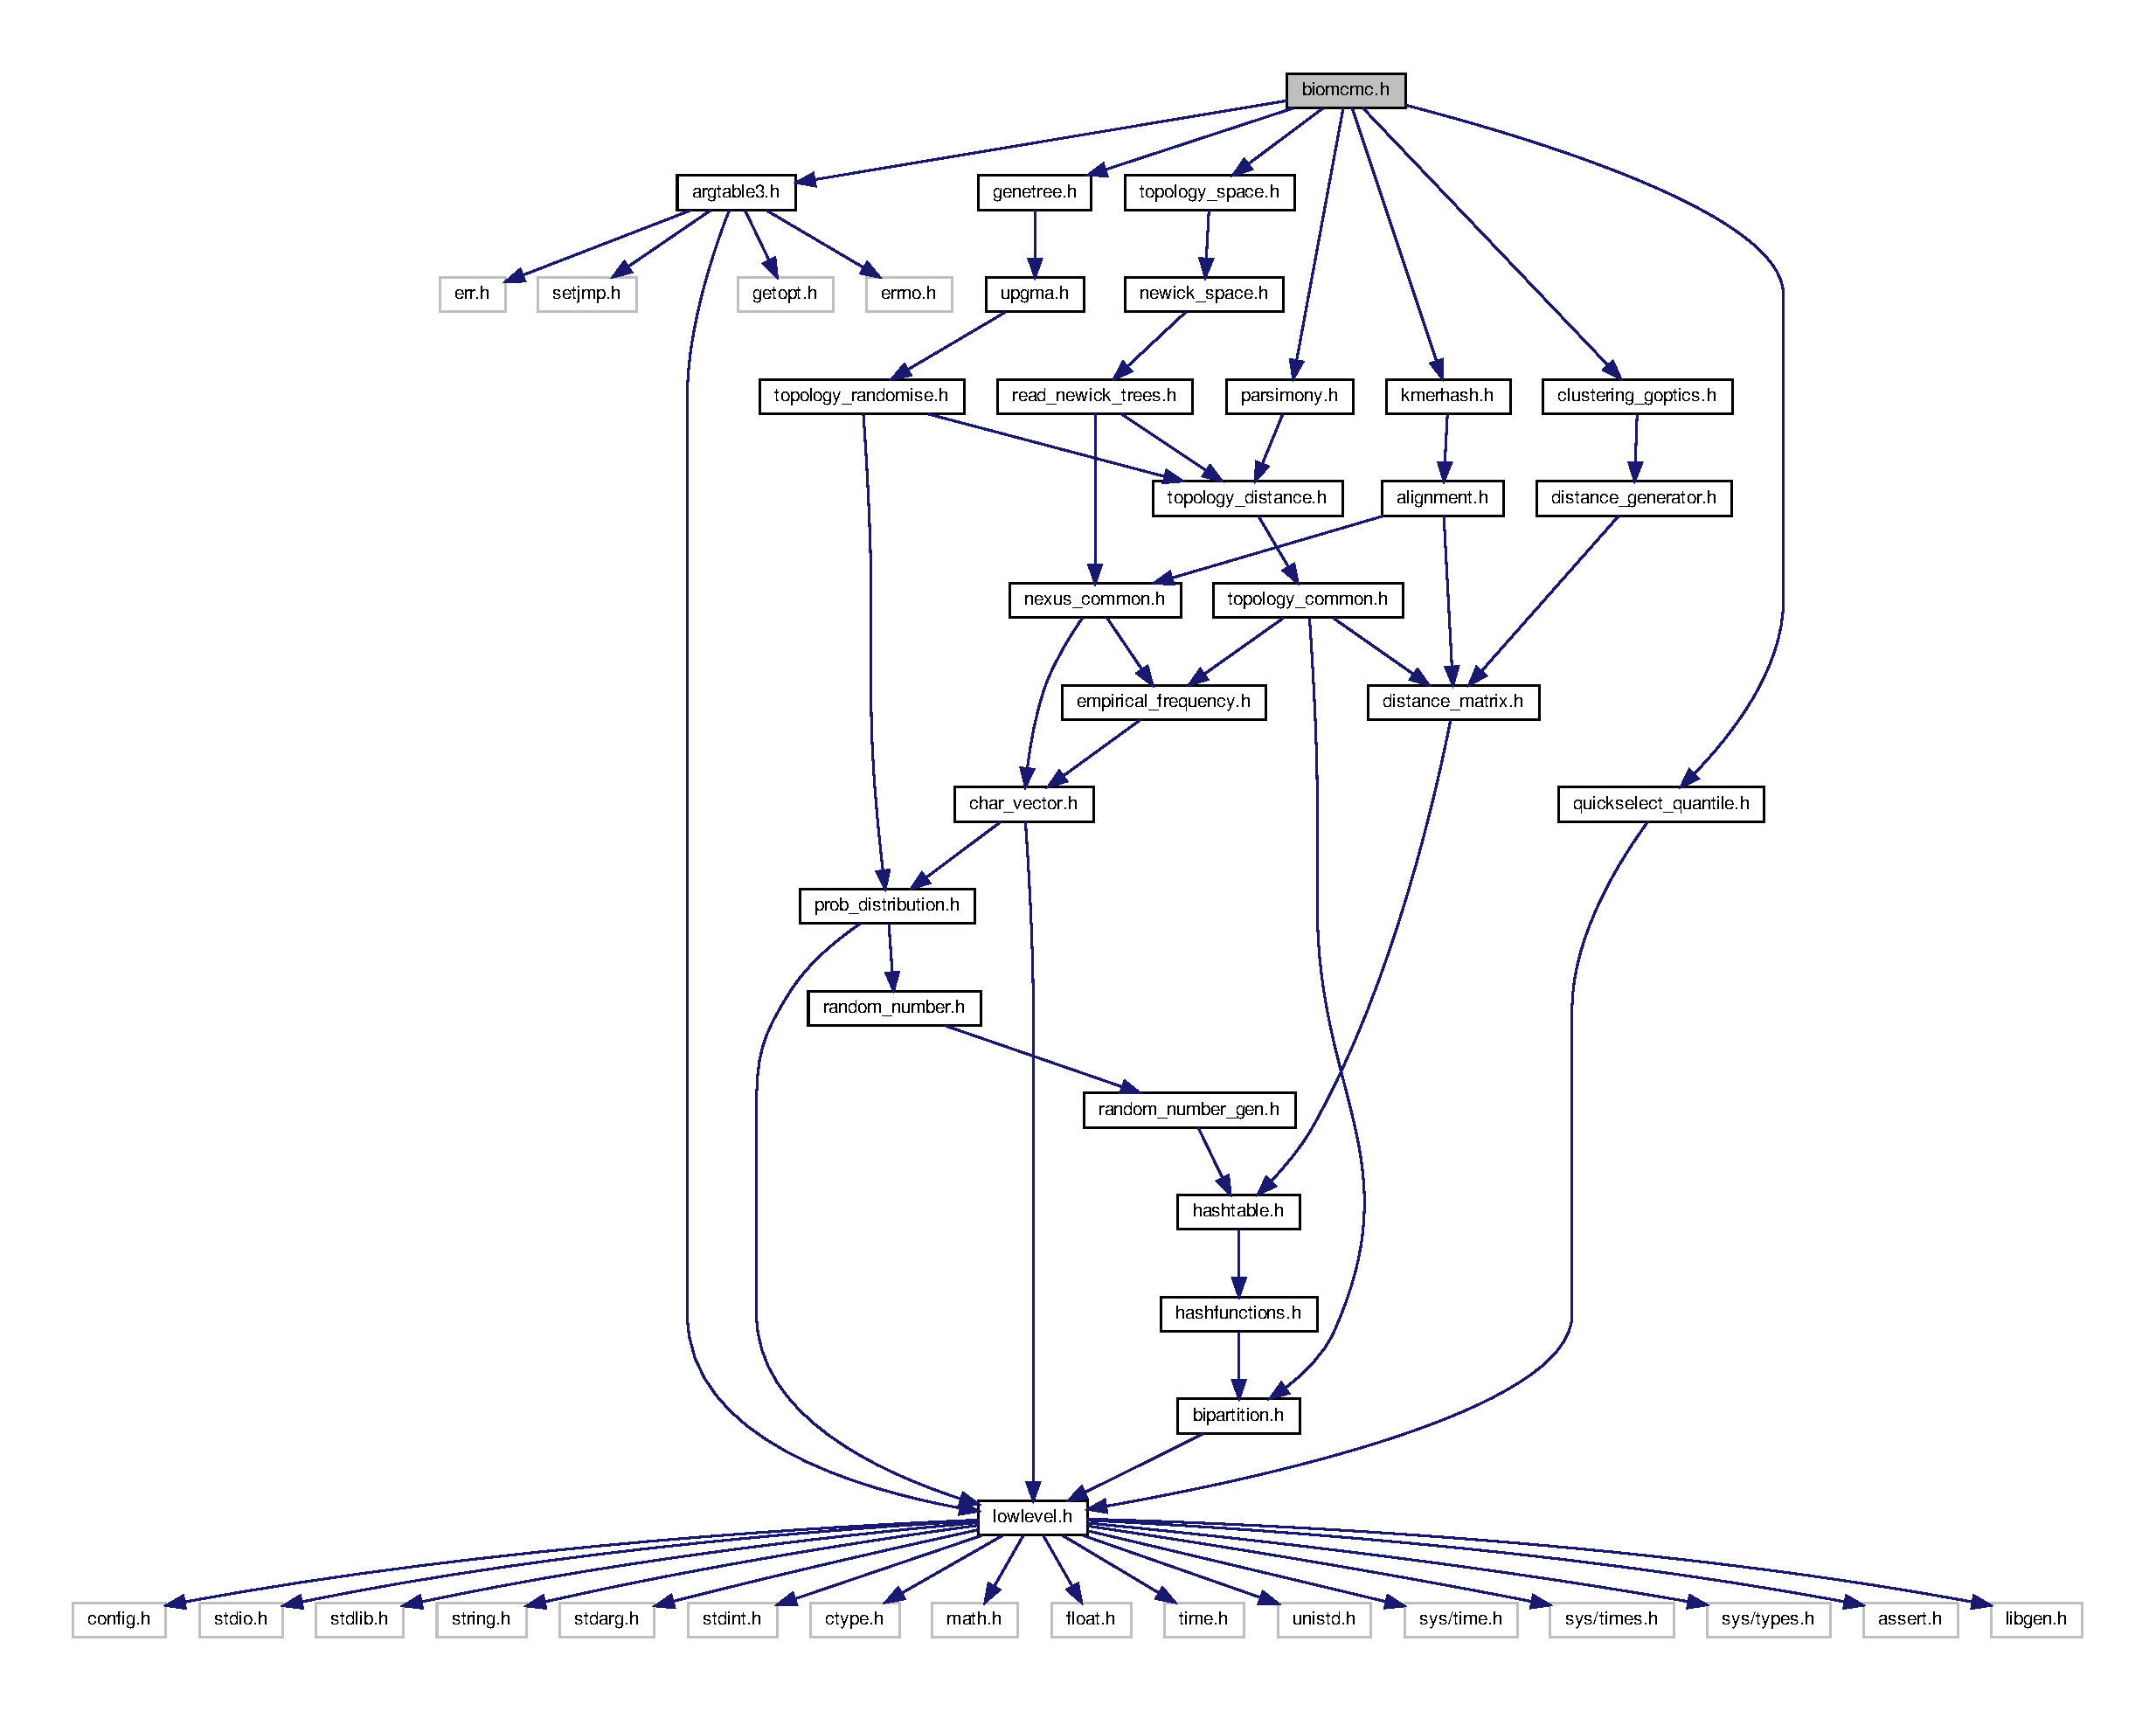
\includegraphics[width=350pt]{biomcmc_8h__incl}
\end{center}
\end{figure}


\subsubsection{Detailed Description}
biomcmc library interface to external programs, specific to super\+\_\+sptree repo. 

The idea is for biomcmc-\/lib is to be general for several sofware, including treesignal and super\+\_\+sptree. This library started branching from the biomcmc library from the guenomu software. It includes the edlib library for sequence pairwise edit distance (\href{http://martinsos.github.io/edlib}{\tt http\+://martinsos.\+github.\+io/edlib}) 
\hypertarget{bipartition_8h}{}\subsection{bipartition.\+h File Reference}
\label{bipartition_8h}\index{bipartition.\+h@{bipartition.\+h}}


Unary/binary operators on arbitrarily-\/sized bitstrings (strings of zeros and ones) like split bipartitions.  


{\ttfamily \#include \char`\"{}lowlevel.\+h\char`\"{}}\newline
Include dependency graph for bipartition.\+h\+:\nopagebreak
\begin{figure}[H]
\begin{center}
\leavevmode
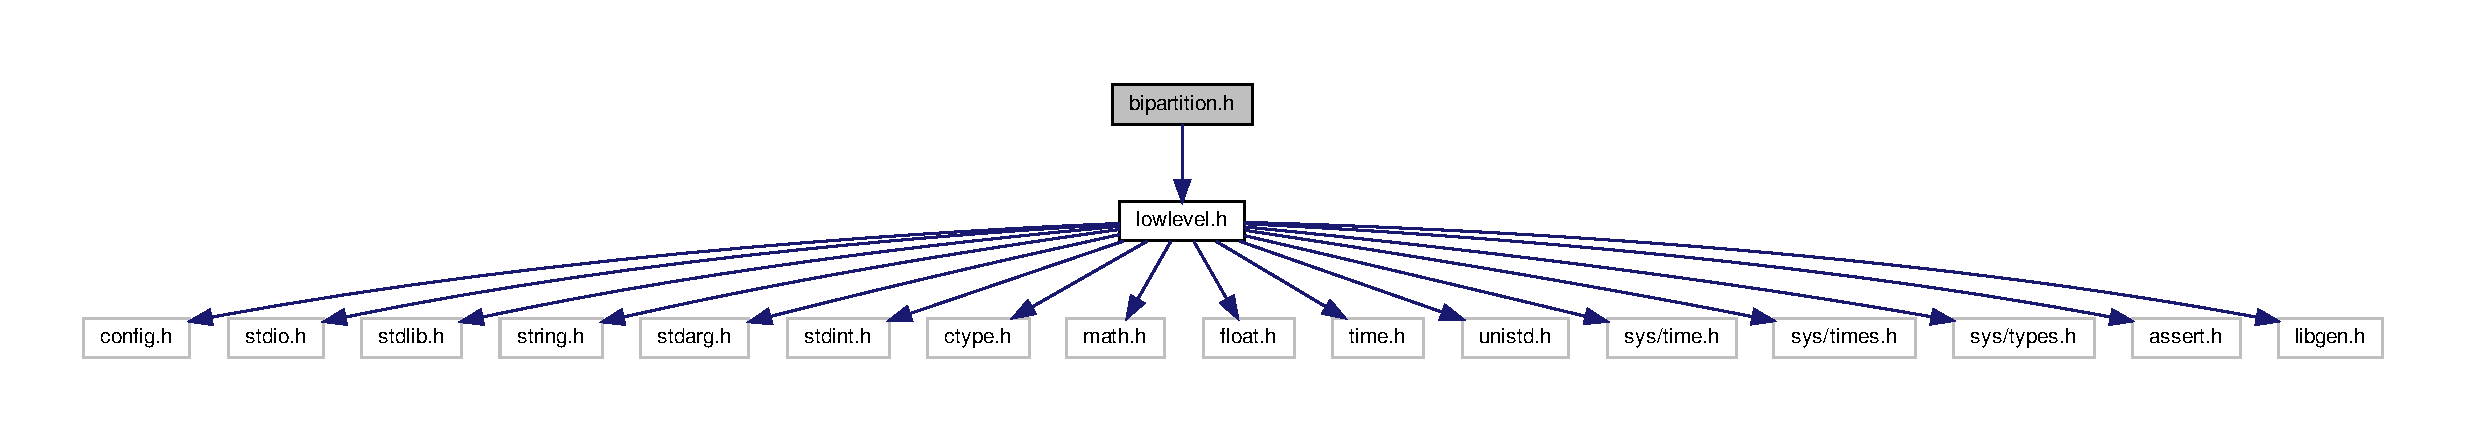
\includegraphics[width=350pt]{bipartition_8h__incl}
\end{center}
\end{figure}
This graph shows which files directly or indirectly include this file\+:\nopagebreak
\begin{figure}[H]
\begin{center}
\leavevmode
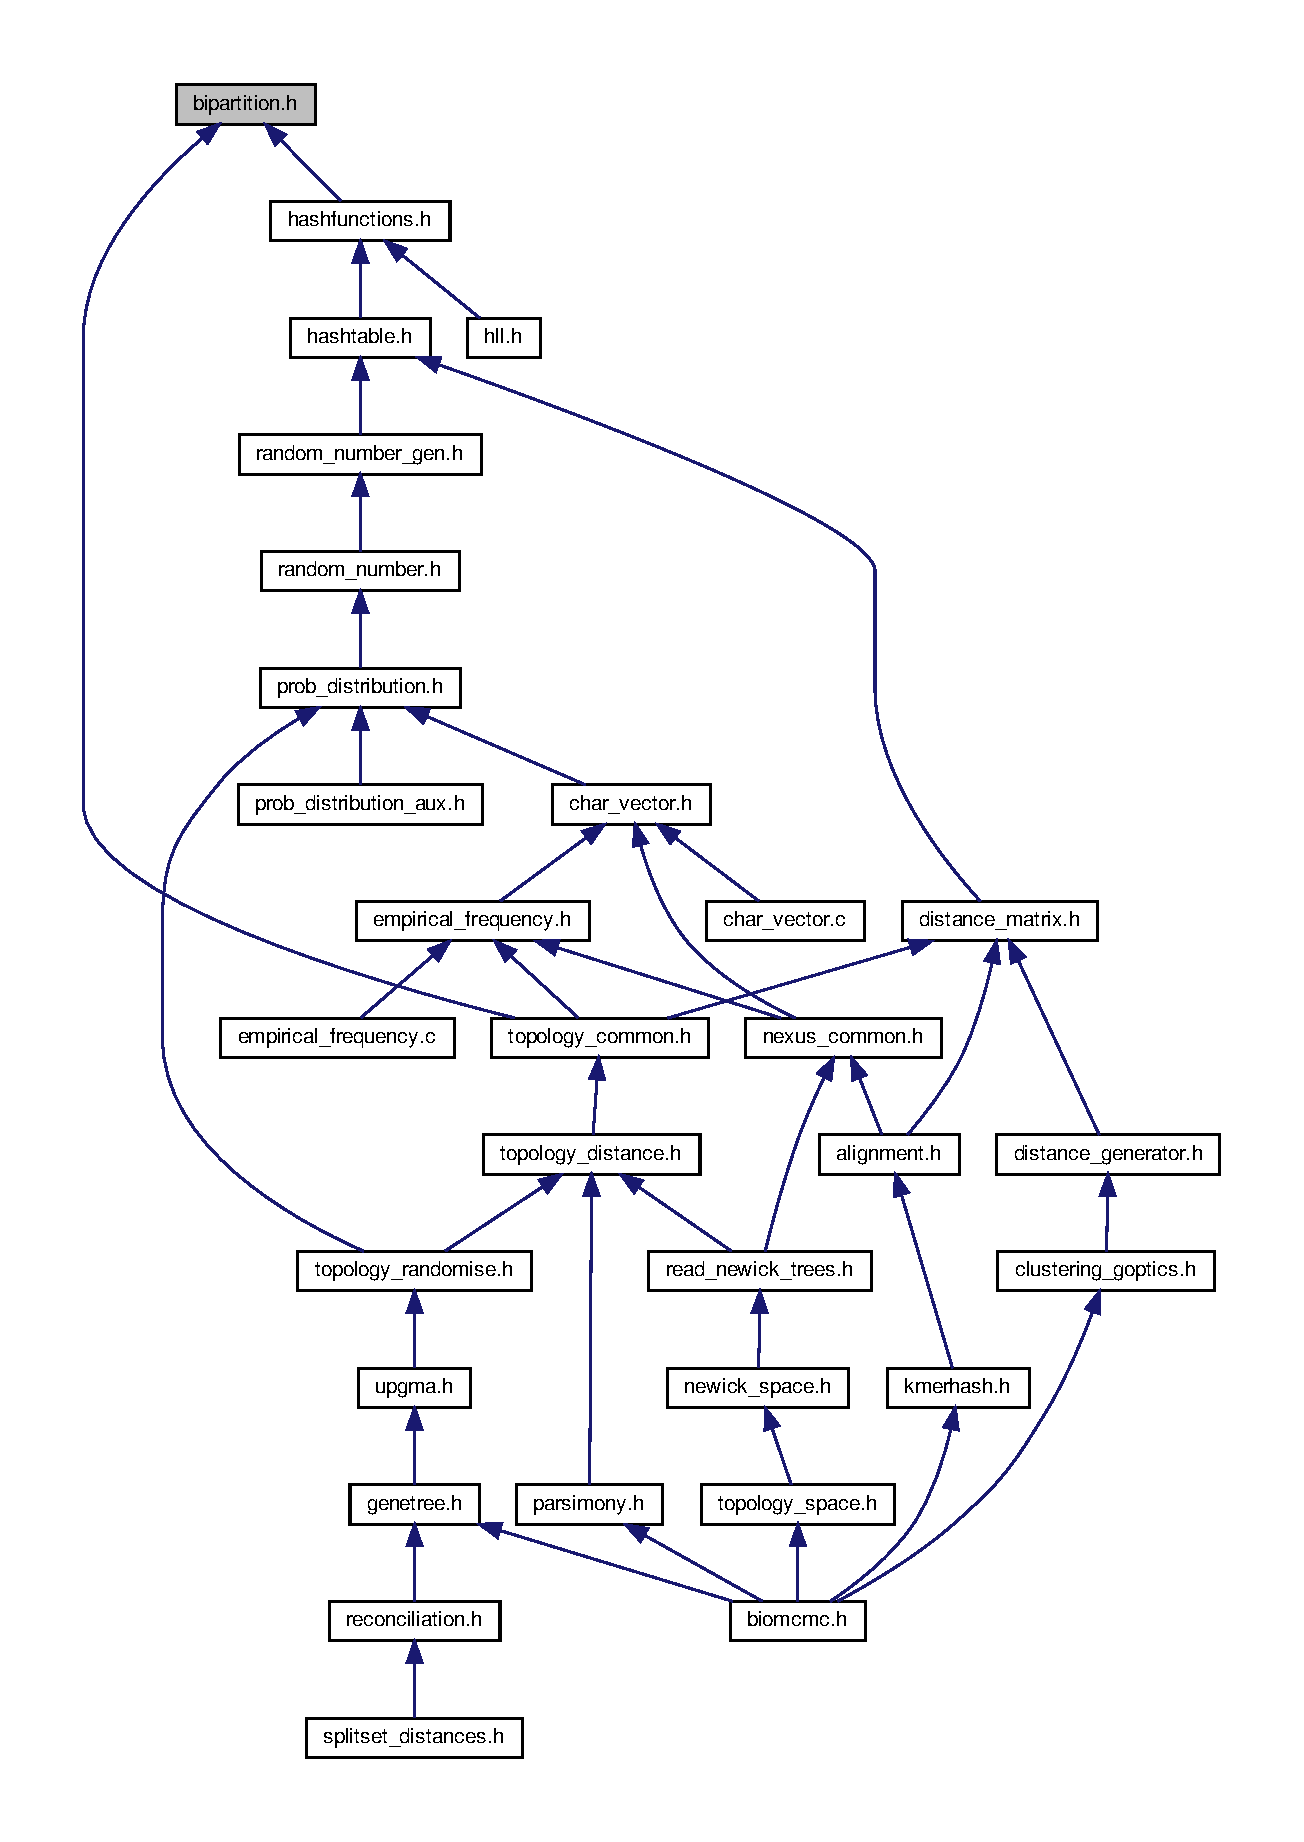
\includegraphics[width=350pt]{bipartition_8h__dep__incl}
\end{center}
\end{figure}
\subsubsection*{Data Structures}
\begin{DoxyCompactItemize}
\item 
struct \hyperlink{structbipartition__struct}{bipartition\+\_\+struct}
\begin{DoxyCompactList}\small\item\em Bit-\/string representation of splits. \end{DoxyCompactList}\item 
struct \hyperlink{structbipsize__struct}{bipsize\+\_\+struct}
\end{DoxyCompactItemize}
\subsubsection*{Typedefs}
\begin{DoxyCompactItemize}
\item 
\mbox{\Hypertarget{bipartition_8h_a306abb015733891f436e9325a3e61716}\label{bipartition_8h_a306abb015733891f436e9325a3e61716}} 
typedef struct \hyperlink{structbipartition__struct}{bipartition\+\_\+struct} $\ast$ {\bfseries bipartition}
\item 
\mbox{\Hypertarget{bipartition_8h_accfcdcb0fabd8a28ab1f40157117ebb6}\label{bipartition_8h_accfcdcb0fabd8a28ab1f40157117ebb6}} 
typedef struct \hyperlink{structbipsize__struct}{bipsize\+\_\+struct} $\ast$ {\bfseries bipsize}
\item 
\mbox{\Hypertarget{bipartition_8h_a84eec7a8b7ee401120ae2970eb3c1260}\label{bipartition_8h_a84eec7a8b7ee401120ae2970eb3c1260}} 
typedef \hyperlink{structbipartition__struct}{bipartition} $\ast$ {\bfseries tripartition}
\end{DoxyCompactItemize}
\subsubsection*{Functions}
\begin{DoxyCompactItemize}
\item 
\hyperlink{structbipartition__struct}{bipartition} \hyperlink{bipartition_8h_a4046e91c94efca27e42476132b89edec}{new\+\_\+bipartition} (int size)
\begin{DoxyCompactList}\small\item\em create a new bipartition (bitstring) capable of storing an arbitrary number of bits and initialize it to zero \end{DoxyCompactList}\item 
\mbox{\Hypertarget{bipartition_8h_a2a4524aef381ee0e194588bf5317439a}\label{bipartition_8h_a2a4524aef381ee0e194588bf5317439a}} 
\hyperlink{structbipsize__struct}{bipsize} \hyperlink{bipartition_8h_a2a4524aef381ee0e194588bf5317439a}{new\+\_\+bipsize} (int size)
\begin{DoxyCompactList}\small\item\em Create a new bipsize, which controls some bipartition sizes. \end{DoxyCompactList}\item 
\mbox{\Hypertarget{bipartition_8h_a79971b17309d8b6dbbd64be3917f1221}\label{bipartition_8h_a79971b17309d8b6dbbd64be3917f1221}} 
\hyperlink{structbipartition__struct}{bipartition} \hyperlink{bipartition_8h_a79971b17309d8b6dbbd64be3917f1221}{new\+\_\+bipartition\+\_\+copy\+\_\+from} (const \hyperlink{structbipartition__struct}{bipartition} from)
\begin{DoxyCompactList}\small\item\em Create a new bipartition (allocate memory) and initialize it from another bipartition. \end{DoxyCompactList}\item 
\mbox{\Hypertarget{bipartition_8h_ac0ba9762329edaf1307a4cb072d58a8c}\label{bipartition_8h_ac0ba9762329edaf1307a4cb072d58a8c}} 
\hyperlink{structbipartition__struct}{bipartition} \hyperlink{bipartition_8h_ac0ba9762329edaf1307a4cb072d58a8c}{new\+\_\+bipartition\+\_\+from\+\_\+bipsize} (\hyperlink{structbipsize__struct}{bipsize} n)
\begin{DoxyCompactList}\small\item\em create new bipartition that will share bipsize -- useful for bipartition vectors \end{DoxyCompactList}\item 
\mbox{\Hypertarget{bipartition_8h_a269368b8696695e9a0ab30a6807f7215}\label{bipartition_8h_a269368b8696695e9a0ab30a6807f7215}} 
void \hyperlink{bipartition_8h_a269368b8696695e9a0ab30a6807f7215}{del\+\_\+bipartition} (\hyperlink{structbipartition__struct}{bipartition} bip)
\begin{DoxyCompactList}\small\item\em free memory allocated by bipartition \end{DoxyCompactList}\item 
\mbox{\Hypertarget{bipartition_8h_a359a51341143b01a6596e07eb38599f8}\label{bipartition_8h_a359a51341143b01a6596e07eb38599f8}} 
void \hyperlink{bipartition_8h_a359a51341143b01a6596e07eb38599f8}{del\+\_\+bipsize} (\hyperlink{structbipsize__struct}{bipsize} n)
\begin{DoxyCompactList}\small\item\em free memory allocated by bipsize \end{DoxyCompactList}\item 
\mbox{\Hypertarget{bipartition_8h_ad9986d7d9721e342f51ccb973d8b05b8}\label{bipartition_8h_ad9986d7d9721e342f51ccb973d8b05b8}} 
void \hyperlink{bipartition_8h_ad9986d7d9721e342f51ccb973d8b05b8}{bipsize\+\_\+resize} (\hyperlink{structbipsize__struct}{bipsize} n, int nbits)
\begin{DoxyCompactList}\small\item\em update the valid number of bits and mask -- e.\+g. when replacing subtrees by leaves in reduced trees \end{DoxyCompactList}\item 
\mbox{\Hypertarget{bipartition_8h_ac1b35d621e3de681fc8adcc59376c15a}\label{bipartition_8h_ac1b35d621e3de681fc8adcc59376c15a}} 
void \hyperlink{bipartition_8h_ac1b35d621e3de681fc8adcc59376c15a}{bipartition\+\_\+initialize} (\hyperlink{structbipartition__struct}{bipartition} bip, int position)
\begin{DoxyCompactList}\small\item\em set all bits to zero except the one at position-\/th bit \end{DoxyCompactList}\item 
\mbox{\Hypertarget{bipartition_8h_a8de2a0287f3dc861078d5a5cb0691727}\label{bipartition_8h_a8de2a0287f3dc861078d5a5cb0691727}} 
void \hyperlink{bipartition_8h_a8de2a0287f3dc861078d5a5cb0691727}{bipartition\+\_\+zero} (\hyperlink{structbipartition__struct}{bipartition} bip)
\begin{DoxyCompactList}\small\item\em set all bits to zero \end{DoxyCompactList}\item 
\mbox{\Hypertarget{bipartition_8h_a733578f349b0cb8baea14357929467ba}\label{bipartition_8h_a733578f349b0cb8baea14357929467ba}} 
void \hyperlink{bipartition_8h_a733578f349b0cb8baea14357929467ba}{bipartition\+\_\+set} (\hyperlink{structbipartition__struct}{bipartition} bip, int position)
\begin{DoxyCompactList}\small\item\em simply set the bit at \char`\"{}position\char`\"{} to one, irrespective of other bits \end{DoxyCompactList}\item 
\mbox{\Hypertarget{bipartition_8h_a867384f907c2a4a937e1f4972a7d4528}\label{bipartition_8h_a867384f907c2a4a937e1f4972a7d4528}} 
void {\bfseries bipartition\+\_\+set\+\_\+lowlevel} (\hyperlink{structbipartition__struct}{bipartition} bip, int i, int j)
\item 
\mbox{\Hypertarget{bipartition_8h_a5a6b3e6c15bddd9e824e4f6fabb4a367}\label{bipartition_8h_a5a6b3e6c15bddd9e824e4f6fabb4a367}} 
void \hyperlink{bipartition_8h_a5a6b3e6c15bddd9e824e4f6fabb4a367}{bipartition\+\_\+unset} (\hyperlink{structbipartition__struct}{bipartition} bip, int position)
\begin{DoxyCompactList}\small\item\em simply unset the bit at \char`\"{}position\char`\"{} (set to zero), irrespective of other bits \end{DoxyCompactList}\item 
\mbox{\Hypertarget{bipartition_8h_ab5dc5e89c9d653be234b0afa18efe892}\label{bipartition_8h_ab5dc5e89c9d653be234b0afa18efe892}} 
void {\bfseries bipartition\+\_\+unset\+\_\+lowlevel} (\hyperlink{structbipartition__struct}{bipartition} bip, int i, int j)
\item 
\mbox{\Hypertarget{bipartition_8h_af43ee65be3d32162462e3db46bfa6c68}\label{bipartition_8h_af43ee65be3d32162462e3db46bfa6c68}} 
void \hyperlink{bipartition_8h_af43ee65be3d32162462e3db46bfa6c68}{bipartition\+\_\+copy} (\hyperlink{structbipartition__struct}{bipartition} to, const \hyperlink{structbipartition__struct}{bipartition} from)
\begin{DoxyCompactList}\small\item\em Copy contents from one bipartition to another. \end{DoxyCompactList}\item 
\mbox{\Hypertarget{bipartition_8h_a08e2a6c72e1b56b0ba7a9305c9571827}\label{bipartition_8h_a08e2a6c72e1b56b0ba7a9305c9571827}} 
void \hyperlink{bipartition_8h_a08e2a6c72e1b56b0ba7a9305c9571827}{bipartition\+\_\+\+OR} (\hyperlink{structbipartition__struct}{bipartition} result, const \hyperlink{structbipartition__struct}{bipartition} b1, const \hyperlink{structbipartition__struct}{bipartition} b2, \hyperlink{lowlevel_8h_a97a80ca1602ebf2303258971a2c938e2}{bool} update\+\_\+count)
\begin{DoxyCompactList}\small\item\em Binary logical OR (\char`\"{}$\vert$\char`\"{}) between b1 and b2, where update\+\_\+count should be true if you need to know the resulting size (slow) or false if you don\textquotesingle{}t care or if b1 and b2 are disjoint (no common elements) \end{DoxyCompactList}\item 
\mbox{\Hypertarget{bipartition_8h_ac8c1099e5da96c71cd4862654a405042}\label{bipartition_8h_ac8c1099e5da96c71cd4862654a405042}} 
void \hyperlink{bipartition_8h_ac8c1099e5da96c71cd4862654a405042}{bipartition\+\_\+\+A\+ND} (\hyperlink{structbipartition__struct}{bipartition} result, const \hyperlink{structbipartition__struct}{bipartition} b1, const \hyperlink{structbipartition__struct}{bipartition} b2, \hyperlink{lowlevel_8h_a97a80ca1602ebf2303258971a2c938e2}{bool} update\+\_\+count)
\begin{DoxyCompactList}\small\item\em Binary logical A\+ND (\char`\"{}\&\char`\"{}) between b1 and b2, update\+\_\+count should be set to false only if you {\bfseries really} don\textquotesingle{}t need to know the number of active bits (e.\+g. sorting, bipartition comparison) \end{DoxyCompactList}\item 
\mbox{\Hypertarget{bipartition_8h_a42d8733818515fcce7867e3a5dd95def}\label{bipartition_8h_a42d8733818515fcce7867e3a5dd95def}} 
void \hyperlink{bipartition_8h_a42d8733818515fcce7867e3a5dd95def}{bipartition\+\_\+\+A\+N\+D\+N\+OT} (\hyperlink{structbipartition__struct}{bipartition} result, const \hyperlink{structbipartition__struct}{bipartition} b1, const \hyperlink{structbipartition__struct}{bipartition} b2, \hyperlink{lowlevel_8h_a97a80ca1602ebf2303258971a2c938e2}{bool} update\+\_\+count)
\begin{DoxyCompactList}\small\item\em Binary logical A\+ND (\char`\"{}\&\char`\"{}) between b1 and $\sim$b2 (N\+OT b2), that is, apply mask b1 on the inverse of b2. \end{DoxyCompactList}\item 
\mbox{\Hypertarget{bipartition_8h_a78342af45538fc650831e5b65248fb5e}\label{bipartition_8h_a78342af45538fc650831e5b65248fb5e}} 
void \hyperlink{bipartition_8h_a78342af45538fc650831e5b65248fb5e}{bipartition\+\_\+\+X\+OR} (\hyperlink{structbipartition__struct}{bipartition} result, const \hyperlink{structbipartition__struct}{bipartition} b1, const \hyperlink{structbipartition__struct}{bipartition} b2, \hyperlink{lowlevel_8h_a97a80ca1602ebf2303258971a2c938e2}{bool} update\+\_\+count)
\begin{DoxyCompactList}\small\item\em Binary logical e\+Xclusive OR (\char`\"{}$^\wedge$\char`\"{}) between b1 and b2, update\+\_\+count should be set to false only if you {\bfseries really} don\textquotesingle{}t need to know the number of active bits (e.\+g. sorting, bipartition comparison) \end{DoxyCompactList}\item 
\mbox{\Hypertarget{bipartition_8h_abc77e0616198ac07ac5d8fe43193f661}\label{bipartition_8h_abc77e0616198ac07ac5d8fe43193f661}} 
void \hyperlink{bipartition_8h_abc77e0616198ac07ac5d8fe43193f661}{bipartition\+\_\+\+X\+O\+R\+N\+OT} (\hyperlink{structbipartition__struct}{bipartition} result, const \hyperlink{structbipartition__struct}{bipartition} b1, const \hyperlink{structbipartition__struct}{bipartition} b2, \hyperlink{lowlevel_8h_a97a80ca1602ebf2303258971a2c938e2}{bool} update\+\_\+count)
\begin{DoxyCompactList}\small\item\em Binary logical e\+Xclusive OR (\char`\"{}$^\wedge$\char`\"{}) between b1 and complement of b2 (that is, N\+OT b2\+: b1 $^\wedge$ $\sim$b2). Used when finding best disagreement (that in this case erases the complement --other side -- of agreement edge) \end{DoxyCompactList}\item 
\mbox{\Hypertarget{bipartition_8h_a2d1bb39a33b970546ac58ffcb046d8d6}\label{bipartition_8h_a2d1bb39a33b970546ac58ffcb046d8d6}} 
void \hyperlink{bipartition_8h_a2d1bb39a33b970546ac58ffcb046d8d6}{bipartition\+\_\+\+N\+OT} (\hyperlink{structbipartition__struct}{bipartition} result, const \hyperlink{structbipartition__struct}{bipartition} bip)
\begin{DoxyCompactList}\small\item\em Unary complement (\char`\"{}$\sim$\char`\"{}) of bipartition. Use with caution, since there is no mask for unused padded bits. \end{DoxyCompactList}\item 
\mbox{\Hypertarget{bipartition_8h_af6cdc9daacc3e05c557f87f26cb2c157}\label{bipartition_8h_af6cdc9daacc3e05c557f87f26cb2c157}} 
void \hyperlink{bipartition_8h_af6cdc9daacc3e05c557f87f26cb2c157}{bipartition\+\_\+count\+\_\+n\+\_\+ones} (const \hyperlink{structbipartition__struct}{bipartition} bip)
\begin{DoxyCompactList}\small\item\em Count the number of active bits (equal to one). Used by \hyperlink{bipartition_8h_ac8c1099e5da96c71cd4862654a405042}{bipartition\+\_\+\+A\+N\+D()} and \hyperlink{bipartition_8h_a78342af45538fc650831e5b65248fb5e}{bipartition\+\_\+\+X\+O\+R()} when update\+\_\+count = true. Please use it parsimoniously since it is as slow as without bitstring representation. \end{DoxyCompactList}\item 
\mbox{\Hypertarget{bipartition_8h_a2cad78ac8b8dcd7daa5372a2f3e6c696}\label{bipartition_8h_a2cad78ac8b8dcd7daa5372a2f3e6c696}} 
void \hyperlink{bipartition_8h_a2cad78ac8b8dcd7daa5372a2f3e6c696}{bipartition\+\_\+to\+\_\+int\+\_\+vector} (const \hyperlink{structbipartition__struct}{bipartition} b, int $\ast$id, int vecsize)
\begin{DoxyCompactList}\small\item\em fill vector id\mbox{[}\mbox{]} with positions of set bits, up to vecsize bits set \end{DoxyCompactList}\item 
\mbox{\Hypertarget{bipartition_8h_a47b6d2c862a9b02cada5eef6f3a96933}\label{bipartition_8h_a47b6d2c862a9b02cada5eef6f3a96933}} 
\hyperlink{lowlevel_8h_a97a80ca1602ebf2303258971a2c938e2}{bool} \hyperlink{bipartition_8h_a47b6d2c862a9b02cada5eef6f3a96933}{bipartition\+\_\+is\+\_\+equal} (const \hyperlink{structbipartition__struct}{bipartition} b1, const \hyperlink{structbipartition__struct}{bipartition} b2)
\begin{DoxyCompactList}\small\item\em Compare equality of two bipartitions. \end{DoxyCompactList}\item 
\mbox{\Hypertarget{bipartition_8h_afeacfd040b535889cf72d43d74284b0d}\label{bipartition_8h_afeacfd040b535889cf72d43d74284b0d}} 
\hyperlink{lowlevel_8h_a97a80ca1602ebf2303258971a2c938e2}{bool} \hyperlink{bipartition_8h_afeacfd040b535889cf72d43d74284b0d}{bipartition\+\_\+is\+\_\+equal\+\_\+bothsides} (const \hyperlink{structbipartition__struct}{bipartition} b1, const \hyperlink{structbipartition__struct}{bipartition} b2)
\begin{DoxyCompactList}\small\item\em Compare if two bipartitions represent the same splits (or they are equal or one is the complement of the other) \end{DoxyCompactList}\item 
\mbox{\Hypertarget{bipartition_8h_a2d26658d417eca17423e332d7adddb8a}\label{bipartition_8h_a2d26658d417eca17423e332d7adddb8a}} 
int \hyperlink{bipartition_8h_a2d26658d417eca17423e332d7adddb8a}{compare\+\_\+bipartitions\+\_\+increasing} (const void $\ast$a1, const void $\ast$a2)
\begin{DoxyCompactList}\small\item\em Bipartitions comparison, to be used by sort() since returns integer and uses (void) \end{DoxyCompactList}\item 
\mbox{\Hypertarget{bipartition_8h_a04f310aa1b02d8ca7ad39bac31d446fd}\label{bipartition_8h_a04f310aa1b02d8ca7ad39bac31d446fd}} 
int \hyperlink{bipartition_8h_a04f310aa1b02d8ca7ad39bac31d446fd}{compare\+\_\+bipartitions\+\_\+decreasing} (const void $\ast$a1, const void $\ast$a2)
\begin{DoxyCompactList}\small\item\em Bipartitions comparison, to be used by sort() since returns integer and uses (void) \end{DoxyCompactList}\item 
\mbox{\Hypertarget{bipartition_8h_a5d7dac5bc657afaa96de811cfe9c6a92}\label{bipartition_8h_a5d7dac5bc657afaa96de811cfe9c6a92}} 
\hyperlink{lowlevel_8h_a97a80ca1602ebf2303258971a2c938e2}{bool} \hyperlink{bipartition_8h_a5d7dac5bc657afaa96de811cfe9c6a92}{bipartition\+\_\+is\+\_\+larger} (const \hyperlink{structbipartition__struct}{bipartition} b1, const \hyperlink{structbipartition__struct}{bipartition} b2)
\begin{DoxyCompactList}\small\item\em Compare sizes of two bipartitions, by number of active bits with ties broken by actual bitstrings. \end{DoxyCompactList}\item 
\mbox{\Hypertarget{bipartition_8h_a1d7aa60b6f49f64b767ee913006b1da6}\label{bipartition_8h_a1d7aa60b6f49f64b767ee913006b1da6}} 
void \hyperlink{bipartition_8h_a1d7aa60b6f49f64b767ee913006b1da6}{bipartition\+\_\+flip\+\_\+to\+\_\+smaller\+\_\+set} (\hyperlink{structbipartition__struct}{bipartition} bip)
\begin{DoxyCompactList}\small\item\em invert ones and zeroes in loco when necessary to assure bipartition has more zeroes than ones \end{DoxyCompactList}\item 
\mbox{\Hypertarget{bipartition_8h_a33c95530b5714285d8ac0362c5231b2e}\label{bipartition_8h_a33c95530b5714285d8ac0362c5231b2e}} 
\hyperlink{lowlevel_8h_a97a80ca1602ebf2303258971a2c938e2}{bool} \hyperlink{bipartition_8h_a33c95530b5714285d8ac0362c5231b2e}{bipartition\+\_\+is\+\_\+bit\+\_\+set} (const \hyperlink{structbipartition__struct}{bipartition} bip, int position)
\begin{DoxyCompactList}\small\item\em Check if position-\/th bit is equal to one or not. \end{DoxyCompactList}\item 
\mbox{\Hypertarget{bipartition_8h_a3c8c51e60cfaef58946fc3aaa66699f3}\label{bipartition_8h_a3c8c51e60cfaef58946fc3aaa66699f3}} 
\hyperlink{lowlevel_8h_a97a80ca1602ebf2303258971a2c938e2}{bool} \hyperlink{bipartition_8h_a3c8c51e60cfaef58946fc3aaa66699f3}{bipartition\+\_\+contains\+\_\+bits} (const \hyperlink{structbipartition__struct}{bipartition} b1, const \hyperlink{structbipartition__struct}{bipartition} b2)
\begin{DoxyCompactList}\small\item\em Check if first bipartition contains all elements of second bipartition (b2 is a subset of b1) \end{DoxyCompactList}\item 
\mbox{\Hypertarget{bipartition_8h_aacb095b009713c046c1a7b9e5a0327dc}\label{bipartition_8h_aacb095b009713c046c1a7b9e5a0327dc}} 
void \hyperlink{bipartition_8h_aacb095b009713c046c1a7b9e5a0327dc}{bipartition\+\_\+print\+\_\+to\+\_\+stdout} (const \hyperlink{structbipartition__struct}{bipartition} b1)
\begin{DoxyCompactList}\small\item\em Print to screen a bit representation of the bipartition (with number of ones at the end) \end{DoxyCompactList}\item 
\mbox{\Hypertarget{bipartition_8h_a806714fe6c29f4c91088507cf78b8905}\label{bipartition_8h_a806714fe6c29f4c91088507cf78b8905}} 
void \hyperlink{bipartition_8h_a806714fe6c29f4c91088507cf78b8905}{bipartition\+\_\+replace\+\_\+bit\+\_\+in\+\_\+vector} (\hyperlink{structbipartition__struct}{bipartition} $\ast$bvec, int n\+\_\+b, int to, int from, \hyperlink{lowlevel_8h_a97a80ca1602ebf2303258971a2c938e2}{bool} reduce)
\begin{DoxyCompactList}\small\item\em replace bit info, copying \textquotesingle{}from\textquotesingle{} one position \textquotesingle{}to\textquotesingle{} another; bool \char`\"{}update\char`\"{} indicates if afterwards size will be reduced \end{DoxyCompactList}\item 
\mbox{\Hypertarget{bipartition_8h_a04f73019b04e2b7283c4b1034d0ab656}\label{bipartition_8h_a04f73019b04e2b7283c4b1034d0ab656}} 
void \hyperlink{bipartition_8h_a04f73019b04e2b7283c4b1034d0ab656}{bipartition\+\_\+resize\+\_\+vector} (\hyperlink{structbipartition__struct}{bipartition} $\ast$bvec, int n\+\_\+b)
\begin{DoxyCompactList}\small\item\em apply mask to last element (useful after manipulations) and count number of bits \end{DoxyCompactList}\item 
\mbox{\Hypertarget{bipartition_8h_ab6400d669335c7cc5ac2e10907d64a9d}\label{bipartition_8h_ab6400d669335c7cc5ac2e10907d64a9d}} 
\hyperlink{structbipartition__struct}{tripartition} \hyperlink{bipartition_8h_ab6400d669335c7cc5ac2e10907d64a9d}{new\+\_\+tripartition} (int nleaves)
\begin{DoxyCompactList}\small\item\em tripartition of a node (a vector with 3 bipartitions, that should not be \textquotesingle{}flipped\textquotesingle{} to smaller set, however) \end{DoxyCompactList}\item 
\mbox{\Hypertarget{bipartition_8h_a7e55ab85d24252191edd3a1768e36816}\label{bipartition_8h_a7e55ab85d24252191edd3a1768e36816}} 
void \hyperlink{bipartition_8h_a7e55ab85d24252191edd3a1768e36816}{del\+\_\+tripartition} (\hyperlink{structbipartition__struct}{tripartition} trip)
\begin{DoxyCompactList}\small\item\em free tripartition space (just 3 bipartitions) \end{DoxyCompactList}\item 
\mbox{\Hypertarget{bipartition_8h_ace9a62f4146cce7467b70b179786a4ae}\label{bipartition_8h_ace9a62f4146cce7467b70b179786a4ae}} 
void \hyperlink{bipartition_8h_ace9a62f4146cce7467b70b179786a4ae}{store\+\_\+tripartition\+\_\+from\+\_\+bipartitions} (\hyperlink{structbipartition__struct}{tripartition} tri, \hyperlink{structbipartition__struct}{bipartition} b1, \hyperlink{structbipartition__struct}{bipartition} b2)
\begin{DoxyCompactList}\small\item\em from node, create tripartition from node-\/$>$left and node-\/$>$right (assuming bipartitions were not \textquotesingle{}flipped\textquotesingle{} yet) \end{DoxyCompactList}\item 
\mbox{\Hypertarget{bipartition_8h_a3c938956ea2a3cc95f0be413e9baa072}\label{bipartition_8h_a3c938956ea2a3cc95f0be413e9baa072}} 
void \hyperlink{bipartition_8h_a3c938956ea2a3cc95f0be413e9baa072}{sort\+\_\+tripartition} (\hyperlink{structbipartition__struct}{tripartition} tri)
\begin{DoxyCompactList}\small\item\em sort order of bipartitions s.\+t. smallest is first \end{DoxyCompactList}\item 
\mbox{\Hypertarget{bipartition_8h_a8eba8eccc761ee9486a4de679448dbc3}\label{bipartition_8h_a8eba8eccc761ee9486a4de679448dbc3}} 
int \hyperlink{bipartition_8h_a8eba8eccc761ee9486a4de679448dbc3}{align\+\_\+tripartitions} (\hyperlink{structbipartition__struct}{tripartition} tp1, \hyperlink{structbipartition__struct}{tripartition} tp2, \hyperlink{structhungarian__struct}{hungarian} h)
\begin{DoxyCompactList}\small\item\em match bipartitions between two nodes and return optimal score (min disagreement) \end{DoxyCompactList}\item 
\mbox{\Hypertarget{bipartition_8h_a8a07a32fc365d03a0ecdd94ecd88340f}\label{bipartition_8h_a8a07a32fc365d03a0ecdd94ecd88340f}} 
\hyperlink{lowlevel_8h_a97a80ca1602ebf2303258971a2c938e2}{bool} \hyperlink{bipartition_8h_a8a07a32fc365d03a0ecdd94ecd88340f}{tripartition\+\_\+is\+\_\+equal} (\hyperlink{structbipartition__struct}{tripartition} tp1, \hyperlink{structbipartition__struct}{tripartition} tp2)
\begin{DoxyCompactList}\small\item\em assuming tripartitions are ordered, check if nodes (represented by tripartitions) are the same \end{DoxyCompactList}\end{DoxyCompactItemize}


\subsubsection{Detailed Description}
Unary/binary operators on arbitrarily-\/sized bitstrings (strings of zeros and ones) like split bipartitions. 



\subsubsection{Function Documentation}
\mbox{\Hypertarget{bipartition_8h_a4046e91c94efca27e42476132b89edec}\label{bipartition_8h_a4046e91c94efca27e42476132b89edec}} 
\index{bipartition.\+h@{bipartition.\+h}!new\+\_\+bipartition@{new\+\_\+bipartition}}
\index{new\+\_\+bipartition@{new\+\_\+bipartition}!bipartition.\+h@{bipartition.\+h}}
\paragraph{\texorpdfstring{new\+\_\+bipartition()}{new\_bipartition()}}
{\footnotesize\ttfamily \hyperlink{structbipartition__struct}{bipartition} new\+\_\+bipartition (\begin{DoxyParamCaption}\item[{int}]{size }\end{DoxyParamCaption})}



create a new bipartition (bitstring) capable of storing an arbitrary number of bits and initialize it to zero 


\begin{DoxyParams}[1]{Parameters}
\mbox{\tt in}  & {\em size} & number of bits of desired bipartition \\
\hline
\end{DoxyParams}
\begin{DoxyReturn}{Returns}
bipartition (opaquely a vector of long long ints) 
\end{DoxyReturn}

\hypertarget{char__vector_8c}{}\subsection{char\+\_\+vector.\+c File Reference}
\label{char__vector_8c}\index{char\+\_\+vector.\+c@{char\+\_\+vector.\+c}}


vector of strings (species names, leaf names, etc.)  


{\ttfamily \#include \char`\"{}char\+\_\+vector.\+h\char`\"{}}\newline
Include dependency graph for char\+\_\+vector.\+c\+:\nopagebreak
\begin{figure}[H]
\begin{center}
\leavevmode
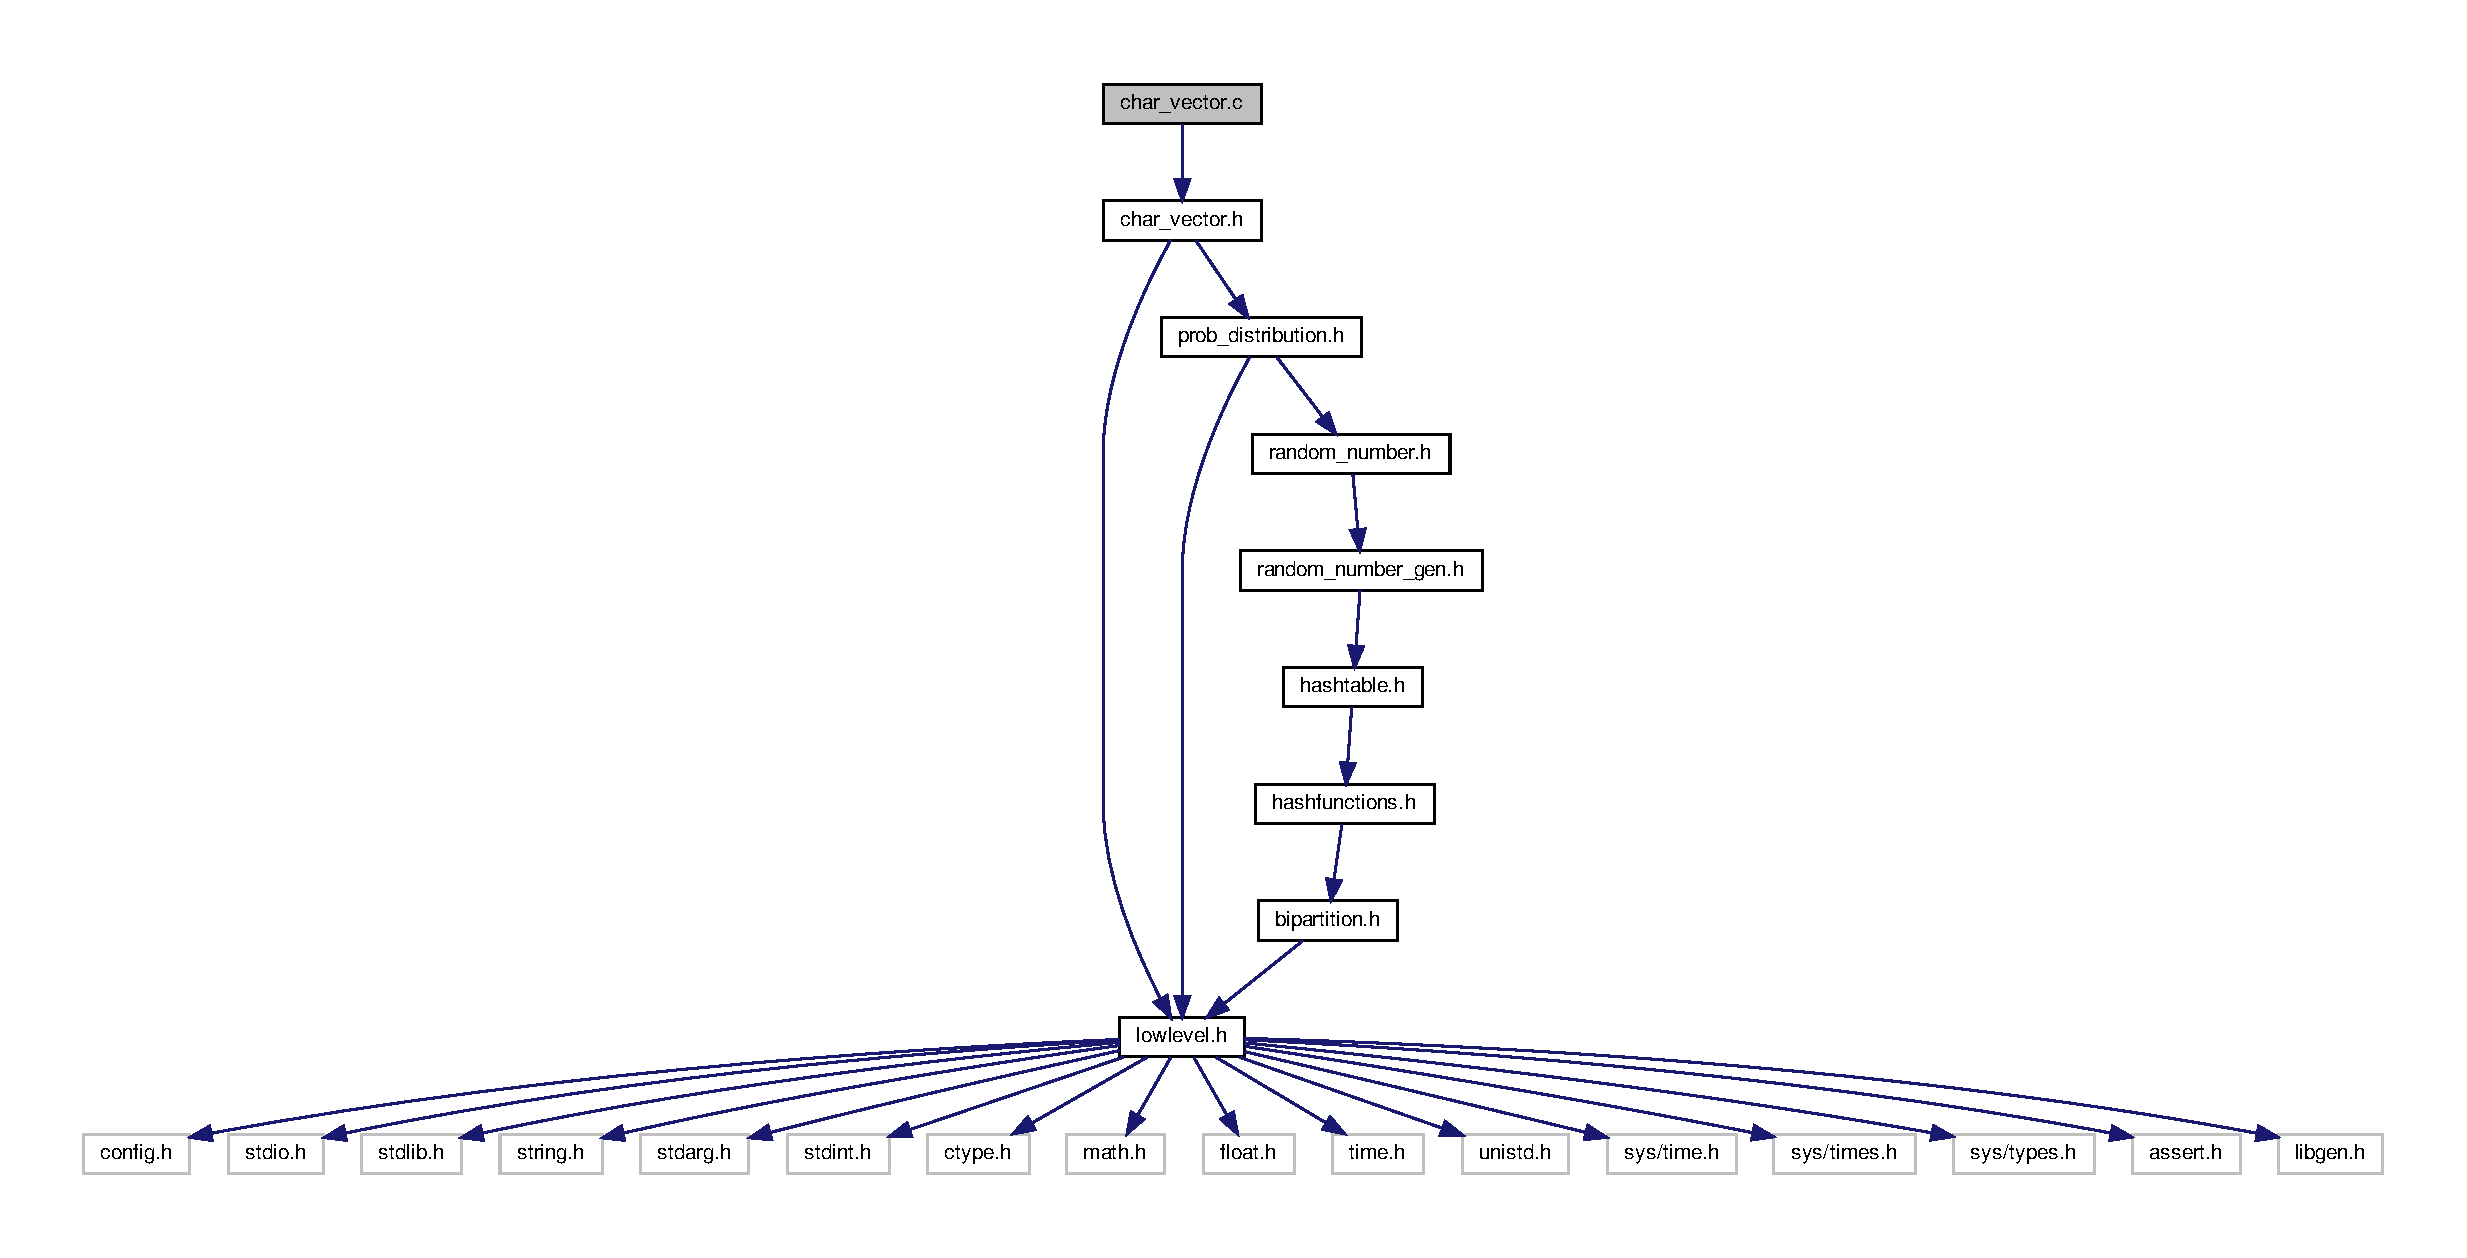
\includegraphics[width=350pt]{char__vector_8c__incl}
\end{center}
\end{figure}
\subsubsection*{Data Structures}
\begin{DoxyCompactItemize}
\item 
struct \hyperlink{structcharvec__str}{charvec\+\_\+str}
\end{DoxyCompactItemize}
\subsubsection*{Macros}
\begin{DoxyCompactItemize}
\item 
\mbox{\Hypertarget{char__vector_8c_af808c6880732c15dd7210159c486ff82}\label{char__vector_8c_af808c6880732c15dd7210159c486ff82}} 
\#define {\bfseries kroundup32}(x)~(-\/-\/(x), (x)$\vert$=(x)$>$$>$1, (x)$\vert$=(x)$>$$>$2, (x)$\vert$=(x)$>$$>$4, (x)$\vert$=(x)$>$$>$8, (x)$\vert$=(x)$>$$>$16, ++(x))
\end{DoxyCompactItemize}
\subsubsection*{Functions}
\begin{DoxyCompactItemize}
\item 
\mbox{\Hypertarget{char__vector_8c_a1baadabbd509958e072a02c9fd20282d}\label{char__vector_8c_a1baadabbd509958e072a02c9fd20282d}} 
int {\bfseries compare\+\_\+charvecstr\+\_\+decreasing} (const void $\ast$a, const void $\ast$b)
\item 
\mbox{\Hypertarget{char__vector_8c_a390bd1b724ff0b3aa14dbc0f3e3314c5}\label{char__vector_8c_a390bd1b724ff0b3aa14dbc0f3e3314c5}} 
int {\bfseries compare\+\_\+charvecstr\+\_\+lexicographic} (const void $\ast$a, const void $\ast$b)
\item 
\mbox{\Hypertarget{char__vector_8c_a36f481d0543cf3ce10d4bc1c42da9fce}\label{char__vector_8c_a36f481d0543cf3ce10d4bc1c42da9fce}} 
\hyperlink{structchar__vector__struct}{char\+\_\+vector} \hyperlink{char__vector_8c_a36f481d0543cf3ce10d4bc1c42da9fce}{new\+\_\+char\+\_\+vector} (int nstrings)
\begin{DoxyCompactList}\small\item\em Create a vector of strings with initial size for each string of zero. \end{DoxyCompactList}\item 
\mbox{\Hypertarget{char__vector_8c_ac54181d27629788a3e27f2b828ae6b7c}\label{char__vector_8c_ac54181d27629788a3e27f2b828ae6b7c}} 
\hyperlink{structchar__vector__struct}{char\+\_\+vector} \hyperlink{char__vector_8c_ac54181d27629788a3e27f2b828ae6b7c}{new\+\_\+char\+\_\+vector\+\_\+big} (int nstrings)
\begin{DoxyCompactList}\small\item\em Create vector of strings, and preparing it to realloc() fewer times; used in conjunction with \textquotesingle{}append\+\_\+big\textquotesingle{}. \end{DoxyCompactList}\item 
\mbox{\Hypertarget{char__vector_8c_aadce8775fbc20432da9bb26065d438bd}\label{char__vector_8c_aadce8775fbc20432da9bb26065d438bd}} 
\hyperlink{structchar__vector__struct}{char\+\_\+vector} \hyperlink{char__vector_8c_aadce8775fbc20432da9bb26065d438bd}{new\+\_\+char\+\_\+vector\+\_\+from\+\_\+valid\+\_\+strings\+\_\+char\+\_\+vector} (\hyperlink{structchar__vector__struct}{char\+\_\+vector} vec, int $\ast$valid, int n\+\_\+valid)
\begin{DoxyCompactList}\small\item\em Create a vector of strings from subset of strings of another char\+\_\+vector. \end{DoxyCompactList}\item 
\mbox{\Hypertarget{char__vector_8c_aa9f15b2b4f004f607e7adc9c7c076568}\label{char__vector_8c_aa9f15b2b4f004f607e7adc9c7c076568}} 
\hyperlink{structchar__vector__struct}{char\+\_\+vector} \hyperlink{char__vector_8c_aa9f15b2b4f004f607e7adc9c7c076568}{new\+\_\+char\+\_\+vector\+\_\+fixed\+\_\+length} (int nstrings, int nchars)
\begin{DoxyCompactList}\small\item\em Create a vector of strings where each string is assigned an initial value of nchars. \end{DoxyCompactList}\item 
\mbox{\Hypertarget{char__vector_8c_ab5793c24b02a77e3983267369de42df9}\label{char__vector_8c_ab5793c24b02a77e3983267369de42df9}} 
void \hyperlink{char__vector_8c_ab5793c24b02a77e3983267369de42df9}{del\+\_\+char\+\_\+vector} (\hyperlink{structchar__vector__struct}{char\+\_\+vector} vec)
\begin{DoxyCompactList}\small\item\em Delete vector of strings only after nobody is using it. \end{DoxyCompactList}\item 
\mbox{\Hypertarget{char__vector_8c_a60c2f8e65e393bea3750f3a647e704a8}\label{char__vector_8c_a60c2f8e65e393bea3750f3a647e704a8}} 
void \hyperlink{char__vector_8c_a60c2f8e65e393bea3750f3a647e704a8}{char\+\_\+vector\+\_\+link\+\_\+string\+\_\+at\+\_\+position} (\hyperlink{structchar__vector__struct}{char\+\_\+vector} vec, const char $\ast$string, int position)
\begin{DoxyCompactList}\small\item\em Link a previously allocated string (to avoid copying all characters) \end{DoxyCompactList}\item 
\mbox{\Hypertarget{char__vector_8c_a8c0ae925a72cbee9733998a99109667c}\label{char__vector_8c_a8c0ae925a72cbee9733998a99109667c}} 
void \hyperlink{char__vector_8c_a8c0ae925a72cbee9733998a99109667c}{char\+\_\+vector\+\_\+add\+\_\+string\+\_\+at\+\_\+position} (\hyperlink{structchar__vector__struct}{char\+\_\+vector} vec, const char $\ast$string, int position)
\begin{DoxyCompactList}\small\item\em Add a new string (vector of characters) at specific location. \end{DoxyCompactList}\item 
\mbox{\Hypertarget{char__vector_8c_ae45bc42b402d2389bcb1dfef736bfe0b}\label{char__vector_8c_ae45bc42b402d2389bcb1dfef736bfe0b}} 
void \hyperlink{char__vector_8c_ae45bc42b402d2389bcb1dfef736bfe0b}{char\+\_\+vector\+\_\+add\+\_\+string} (\hyperlink{structchar__vector__struct}{char\+\_\+vector} vec, const char $\ast$string)
\begin{DoxyCompactList}\small\item\em Add a new string (vector of characters) at next available location. \end{DoxyCompactList}\item 
\mbox{\Hypertarget{char__vector_8c_a5e8e36faace92faa8fa6b572205159d1}\label{char__vector_8c_a5e8e36faace92faa8fa6b572205159d1}} 
void \hyperlink{char__vector_8c_a5e8e36faace92faa8fa6b572205159d1}{char\+\_\+vector\+\_\+append\+\_\+string\+\_\+at\+\_\+position} (\hyperlink{structchar__vector__struct}{char\+\_\+vector} vec, const char $\ast$string, int position)
\begin{DoxyCompactList}\small\item\em Append string at the end of existing string at location. \end{DoxyCompactList}\item 
\mbox{\Hypertarget{char__vector_8c_ab33f21fe78327658e035e6ed0e69e7bd}\label{char__vector_8c_ab33f21fe78327658e035e6ed0e69e7bd}} 
void \hyperlink{char__vector_8c_ab33f21fe78327658e035e6ed0e69e7bd}{char\+\_\+vector\+\_\+append\+\_\+string} (\hyperlink{structchar__vector__struct}{char\+\_\+vector} vec, const char $\ast$string)
\begin{DoxyCompactList}\small\item\em Append string at the end of existing string at most recently used location. \end{DoxyCompactList}\item 
\mbox{\Hypertarget{char__vector_8c_a13107fb84cca2e3ef7a4bcfa7a12ac62}\label{char__vector_8c_a13107fb84cca2e3ef7a4bcfa7a12ac62}} 
void \hyperlink{char__vector_8c_a13107fb84cca2e3ef7a4bcfa7a12ac62}{char\+\_\+vector\+\_\+append\+\_\+string\+\_\+big\+\_\+at\+\_\+position} (\hyperlink{structchar__vector__struct}{char\+\_\+vector} vec, const char $\ast$string, int position)
\begin{DoxyCompactList}\small\item\em Append strings like before, but doubling allocation space if insufficient (reduces calls to realloc() ) \end{DoxyCompactList}\item 
\mbox{\Hypertarget{char__vector_8c_aabb37a91468498e1d957a97265af82f4}\label{char__vector_8c_aabb37a91468498e1d957a97265af82f4}} 
void {\bfseries char\+\_\+vector\+\_\+append\+\_\+string\+\_\+big} (\hyperlink{structchar__vector__struct}{char\+\_\+vector} vec, const char $\ast$string)
\item 
\mbox{\Hypertarget{char__vector_8c_adead2adb31107ea801bcb35500760968}\label{char__vector_8c_adead2adb31107ea801bcb35500760968}} 
void {\bfseries char\+\_\+vector\+\_\+finalise\+\_\+big} (\hyperlink{structchar__vector__struct}{char\+\_\+vector} vec)
\item 
\mbox{\Hypertarget{char__vector_8c_a49e07c436cc8b227d49b0033ea0ade01}\label{char__vector_8c_a49e07c436cc8b227d49b0033ea0ade01}} 
void \hyperlink{char__vector_8c_a49e07c436cc8b227d49b0033ea0ade01}{char\+\_\+vector\+\_\+expand\+\_\+nstrings} (\hyperlink{structchar__vector__struct}{char\+\_\+vector} vec, int new\+\_\+size)
\begin{DoxyCompactList}\small\item\em Increase size of vector of strings (called automatically by other functions) \end{DoxyCompactList}\item 
\mbox{\Hypertarget{char__vector_8c_af0dff4c21127fb84f098c90b25da7f57}\label{char__vector_8c_af0dff4c21127fb84f098c90b25da7f57}} 
void \hyperlink{char__vector_8c_af0dff4c21127fb84f098c90b25da7f57}{char\+\_\+vector\+\_\+reorder\+\_\+strings\+\_\+from\+\_\+external\+\_\+order} (\hyperlink{structchar__vector__struct}{char\+\_\+vector} vec, int $\ast$order)
\begin{DoxyCompactList}\small\item\em update order of strings in vector based on a vector of new positions \end{DoxyCompactList}\item 
\mbox{\Hypertarget{char__vector_8c_af643e161413e7e5609ea4fd6d8b9a339}\label{char__vector_8c_af643e161413e7e5609ea4fd6d8b9a339}} 
int \hyperlink{char__vector_8c_af643e161413e7e5609ea4fd6d8b9a339}{char\+\_\+vector\+\_\+remove\+\_\+empty\+\_\+strings} (\hyperlink{structchar__vector__struct}{char\+\_\+vector} vec)
\begin{DoxyCompactList}\small\item\em Reduce size of vector of strings by removing empty strings (returns number of empty strings) \end{DoxyCompactList}\item 
\mbox{\Hypertarget{char__vector_8c_aef03793195d0812db94a8e3e72d5f970}\label{char__vector_8c_aef03793195d0812db94a8e3e72d5f970}} 
int \hyperlink{char__vector_8c_aef03793195d0812db94a8e3e72d5f970}{char\+\_\+vector\+\_\+remove\+\_\+duplicate\+\_\+strings} (\hyperlink{structchar__vector__struct}{char\+\_\+vector} vec)
\begin{DoxyCompactList}\small\item\em Remove identical strings and resizes \hyperlink{structchar__vector__struct}{char\+\_\+vector\+\_\+struct}. \end{DoxyCompactList}\item 
\mbox{\Hypertarget{char__vector_8c_ad39fe4da934e84c0ee80c911dc097d90}\label{char__vector_8c_ad39fe4da934e84c0ee80c911dc097d90}} 
void \hyperlink{char__vector_8c_ad39fe4da934e84c0ee80c911dc097d90}{char\+\_\+vector\+\_\+reduce\+\_\+to\+\_\+valid\+\_\+strings} (\hyperlink{structchar__vector__struct}{char\+\_\+vector} vec, int $\ast$valid, int n\+\_\+valid)
\begin{DoxyCompactList}\small\item\em reduce char\+\_\+string\+\_\+struct to only those elements indexed by valid\mbox{[}\mbox{]} \end{DoxyCompactList}\item 
\mbox{\Hypertarget{char__vector_8c_af4c02ca811d97b2ecf75290dc59ca085}\label{char__vector_8c_af4c02ca811d97b2ecf75290dc59ca085}} 
void \hyperlink{char__vector_8c_af4c02ca811d97b2ecf75290dc59ca085}{char\+\_\+vector\+\_\+reorder\+\_\+by\+\_\+size\+\_\+or\+\_\+lexicographically} (\hyperlink{structchar__vector__struct}{char\+\_\+vector} vec, \hyperlink{lowlevel_8h_a97a80ca1602ebf2303258971a2c938e2}{bool} lexico, int $\ast$order)
\begin{DoxyCompactList}\small\item\em Order \hyperlink{structchar__vector__struct}{char\+\_\+vector\+\_\+struct} elements from longer string to smaller, or lexicographically; can be used after calling \hyperlink{nexus__common_8h_a70de40a0b5802b9872d5eb6578adf2ae}{new\+\_\+char\+\_\+vector\+\_\+from\+\_\+file()} but if topology etc. are associated to it, then order\mbox{[}\mbox{]} must be externally defined and will have new locations, to keep track of changes. \end{DoxyCompactList}\item 
\mbox{\Hypertarget{char__vector_8c_a2f2d3371e5c7aa994ef5d9a8af923333}\label{char__vector_8c_a2f2d3371e5c7aa994ef5d9a8af923333}} 
\hyperlink{lowlevel_8h_a97a80ca1602ebf2303258971a2c938e2}{bool} \hyperlink{char__vector_8c_a2f2d3371e5c7aa994ef5d9a8af923333}{char\+\_\+vector\+\_\+link\+\_\+address\+\_\+if\+\_\+identical} (\hyperlink{structchar__vector__struct}{char\+\_\+vector} $\ast$v1, \hyperlink{structchar__vector__struct}{char\+\_\+vector} $\ast$v2)
\begin{DoxyCompactList}\small\item\em If the two char\+\_\+vectors are identical (same strings in same order), then delete one and make it point to the other one. \end{DoxyCompactList}\item 
void \hyperlink{char__vector_8c_a69440499315ab425fb2849e816ab3034}{index\+\_\+species\+\_\+gene\+\_\+char\+\_\+vectors} (\hyperlink{structchar__vector__struct}{char\+\_\+vector} species, \hyperlink{structchar__vector__struct}{char\+\_\+vector} gene, int $\ast$sp\+\_\+idx\+\_\+in\+\_\+gene, int $\ast$order\+\_\+external)
\begin{DoxyCompactList}\small\item\em find occurences of species-\/$>$string\mbox{[}\mbox{]} inside gene-\/$>$string\mbox{[}\mbox{]} filling indexes in sp\+\_\+idx\+\_\+in\+\_\+gene. \end{DoxyCompactList}\item 
\mbox{\Hypertarget{char__vector_8c_a1b81b79044fa296f110a4eb8671e5924}\label{char__vector_8c_a1b81b79044fa296f110a4eb8671e5924}} 
void {\bfseries update\+\_\+species\+\_\+count\+\_\+from\+\_\+gene\+\_\+char\+\_\+vector} (\hyperlink{structchar__vector__struct}{char\+\_\+vector} species, \hyperlink{structchar__vector__struct}{char\+\_\+vector} gene, int $\ast$sp\+\_\+count)
\end{DoxyCompactItemize}


\subsubsection{Detailed Description}
vector of strings (species names, leaf names, etc.) 



\subsubsection{Function Documentation}
\mbox{\Hypertarget{char__vector_8c_a69440499315ab425fb2849e816ab3034}\label{char__vector_8c_a69440499315ab425fb2849e816ab3034}} 
\index{char\+\_\+vector.\+c@{char\+\_\+vector.\+c}!index\+\_\+species\+\_\+gene\+\_\+char\+\_\+vectors@{index\+\_\+species\+\_\+gene\+\_\+char\+\_\+vectors}}
\index{index\+\_\+species\+\_\+gene\+\_\+char\+\_\+vectors@{index\+\_\+species\+\_\+gene\+\_\+char\+\_\+vectors}!char\+\_\+vector.\+c@{char\+\_\+vector.\+c}}
\paragraph{\texorpdfstring{index\+\_\+species\+\_\+gene\+\_\+char\+\_\+vectors()}{index\_species\_gene\_char\_vectors()}}
{\footnotesize\ttfamily void index\+\_\+species\+\_\+gene\+\_\+char\+\_\+vectors (\begin{DoxyParamCaption}\item[{\hyperlink{structchar__vector__struct}{char\+\_\+vector}}]{species,  }\item[{\hyperlink{structchar__vector__struct}{char\+\_\+vector}}]{gene,  }\item[{int $\ast$}]{sp\+\_\+idx\+\_\+in\+\_\+gene,  }\item[{int $\ast$}]{order\+\_\+external }\end{DoxyParamCaption})}



find occurences of species-\/$>$string\mbox{[}\mbox{]} inside gene-\/$>$string\mbox{[}\mbox{]} filling indexes in sp\+\_\+idx\+\_\+in\+\_\+gene. 

The species are taxon names which may be associated with topologies or alignments, such that we can not reorder its elements here (without also modifing e.\+g. tree leaves). But ordering from longer to shorter is essential for pattern finding, so it is assumed that the char\+\_\+vector is already sorted U\+N\+L\+E\+SS user provides the ordering. 
\hypertarget{char__vector_8h}{}\subsection{char\+\_\+vector.\+h File Reference}
\label{char__vector_8h}\index{char\+\_\+vector.\+h@{char\+\_\+vector.\+h}}


list of strings (each string is a vector of chars)  


{\ttfamily \#include \char`\"{}lowlevel.\+h\char`\"{}}\newline
{\ttfamily \#include \char`\"{}prob\+\_\+distribution.\+h\char`\"{}}\newline
Include dependency graph for char\+\_\+vector.\+h\+:\nopagebreak
\begin{figure}[H]
\begin{center}
\leavevmode
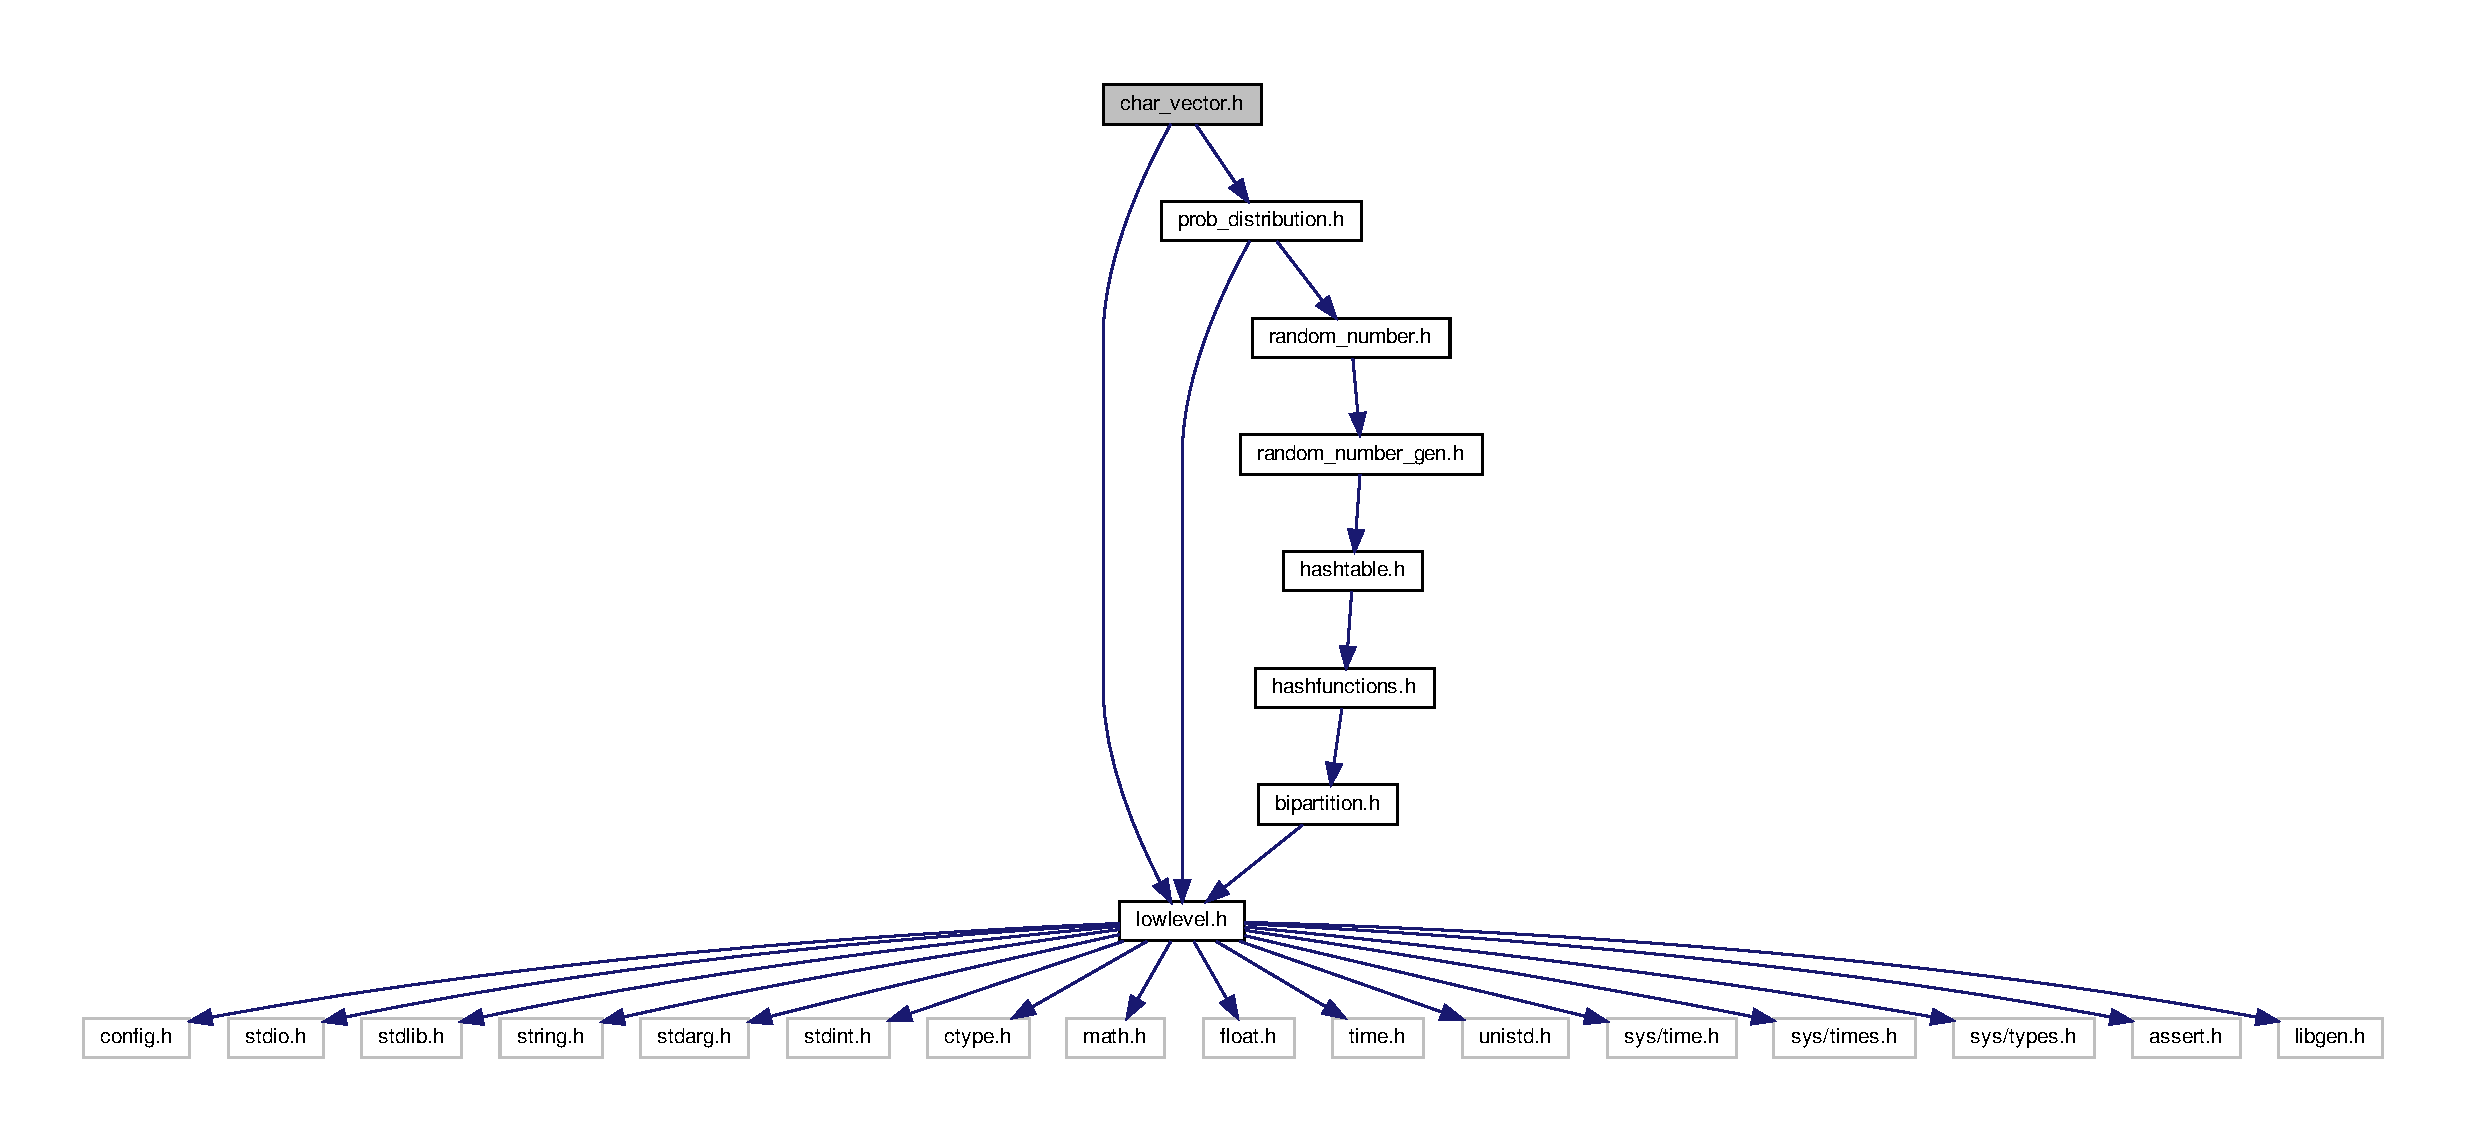
\includegraphics[width=350pt]{char__vector_8h__incl}
\end{center}
\end{figure}
This graph shows which files directly or indirectly include this file\+:\nopagebreak
\begin{figure}[H]
\begin{center}
\leavevmode
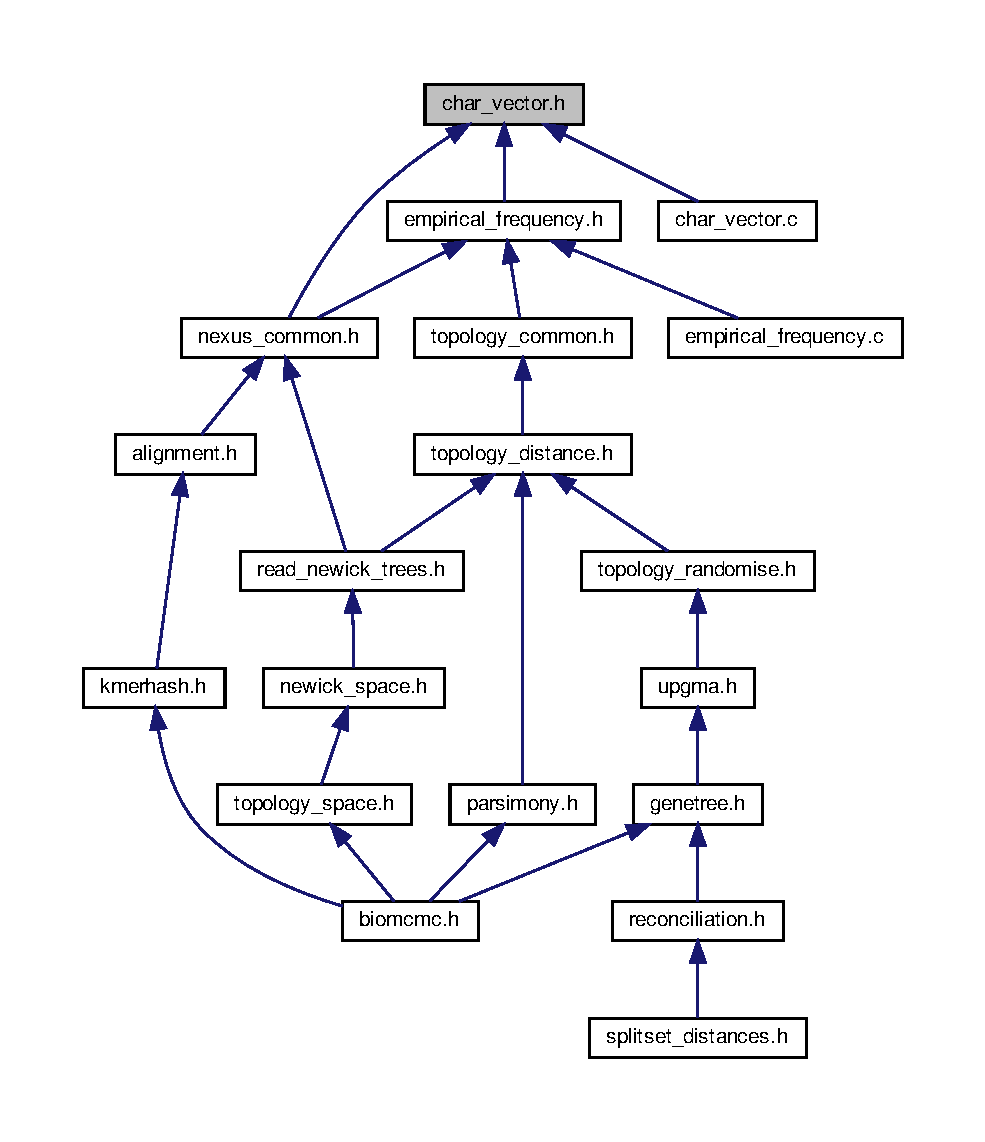
\includegraphics[width=350pt]{char__vector_8h__dep__incl}
\end{center}
\end{figure}
\subsubsection*{Data Structures}
\begin{DoxyCompactItemize}
\item 
struct \hyperlink{structchar__vector__struct}{char\+\_\+vector\+\_\+struct}
\begin{DoxyCompactList}\small\item\em vector of strings (char vectors) of variable length \end{DoxyCompactList}\end{DoxyCompactItemize}
\subsubsection*{Typedefs}
\begin{DoxyCompactItemize}
\item 
\mbox{\Hypertarget{char__vector_8h_a7305316d7c92af95826d16cd2642fe08}\label{char__vector_8h_a7305316d7c92af95826d16cd2642fe08}} 
typedef struct \hyperlink{structchar__vector__struct}{char\+\_\+vector\+\_\+struct} $\ast$ {\bfseries char\+\_\+vector}
\end{DoxyCompactItemize}
\subsubsection*{Functions}
\begin{DoxyCompactItemize}
\item 
\mbox{\Hypertarget{char__vector_8h_a36f481d0543cf3ce10d4bc1c42da9fce}\label{char__vector_8h_a36f481d0543cf3ce10d4bc1c42da9fce}} 
\hyperlink{structchar__vector__struct}{char\+\_\+vector} \hyperlink{char__vector_8h_a36f481d0543cf3ce10d4bc1c42da9fce}{new\+\_\+char\+\_\+vector} (int nstrings)
\begin{DoxyCompactList}\small\item\em Create a vector of strings with initial size for each string of zero. \end{DoxyCompactList}\item 
\mbox{\Hypertarget{char__vector_8h_ac54181d27629788a3e27f2b828ae6b7c}\label{char__vector_8h_ac54181d27629788a3e27f2b828ae6b7c}} 
\hyperlink{structchar__vector__struct}{char\+\_\+vector} \hyperlink{char__vector_8h_ac54181d27629788a3e27f2b828ae6b7c}{new\+\_\+char\+\_\+vector\+\_\+big} (int nstrings)
\begin{DoxyCompactList}\small\item\em Create vector of strings, and preparing it to realloc() fewer times; used in conjunction with \textquotesingle{}append\+\_\+big\textquotesingle{}. \end{DoxyCompactList}\item 
\mbox{\Hypertarget{char__vector_8h_aadce8775fbc20432da9bb26065d438bd}\label{char__vector_8h_aadce8775fbc20432da9bb26065d438bd}} 
\hyperlink{structchar__vector__struct}{char\+\_\+vector} \hyperlink{char__vector_8h_aadce8775fbc20432da9bb26065d438bd}{new\+\_\+char\+\_\+vector\+\_\+from\+\_\+valid\+\_\+strings\+\_\+char\+\_\+vector} (\hyperlink{structchar__vector__struct}{char\+\_\+vector} vec, int $\ast$valid, int n\+\_\+valid)
\begin{DoxyCompactList}\small\item\em Create a vector of strings from subset of strings of another char\+\_\+vector. \end{DoxyCompactList}\item 
\mbox{\Hypertarget{char__vector_8h_aa9f15b2b4f004f607e7adc9c7c076568}\label{char__vector_8h_aa9f15b2b4f004f607e7adc9c7c076568}} 
\hyperlink{structchar__vector__struct}{char\+\_\+vector} \hyperlink{char__vector_8h_aa9f15b2b4f004f607e7adc9c7c076568}{new\+\_\+char\+\_\+vector\+\_\+fixed\+\_\+length} (int nstrings, int nchars)
\begin{DoxyCompactList}\small\item\em Create a vector of strings where each string is assigned an initial value of nchars. \end{DoxyCompactList}\item 
\mbox{\Hypertarget{char__vector_8h_ab5793c24b02a77e3983267369de42df9}\label{char__vector_8h_ab5793c24b02a77e3983267369de42df9}} 
void \hyperlink{char__vector_8h_ab5793c24b02a77e3983267369de42df9}{del\+\_\+char\+\_\+vector} (\hyperlink{structchar__vector__struct}{char\+\_\+vector} vec)
\begin{DoxyCompactList}\small\item\em Delete vector of strings only after nobody is using it. \end{DoxyCompactList}\item 
\mbox{\Hypertarget{char__vector_8h_a60c2f8e65e393bea3750f3a647e704a8}\label{char__vector_8h_a60c2f8e65e393bea3750f3a647e704a8}} 
void \hyperlink{char__vector_8h_a60c2f8e65e393bea3750f3a647e704a8}{char\+\_\+vector\+\_\+link\+\_\+string\+\_\+at\+\_\+position} (\hyperlink{structchar__vector__struct}{char\+\_\+vector} vec, const char $\ast$string, int position)
\begin{DoxyCompactList}\small\item\em Link a previously allocated string (to avoid copying all characters) \end{DoxyCompactList}\item 
\mbox{\Hypertarget{char__vector_8h_a8c0ae925a72cbee9733998a99109667c}\label{char__vector_8h_a8c0ae925a72cbee9733998a99109667c}} 
void \hyperlink{char__vector_8h_a8c0ae925a72cbee9733998a99109667c}{char\+\_\+vector\+\_\+add\+\_\+string\+\_\+at\+\_\+position} (\hyperlink{structchar__vector__struct}{char\+\_\+vector} vec, const char $\ast$string, int position)
\begin{DoxyCompactList}\small\item\em Add a new string (vector of characters) at specific location. \end{DoxyCompactList}\item 
\mbox{\Hypertarget{char__vector_8h_ae45bc42b402d2389bcb1dfef736bfe0b}\label{char__vector_8h_ae45bc42b402d2389bcb1dfef736bfe0b}} 
void \hyperlink{char__vector_8h_ae45bc42b402d2389bcb1dfef736bfe0b}{char\+\_\+vector\+\_\+add\+\_\+string} (\hyperlink{structchar__vector__struct}{char\+\_\+vector} vec, const char $\ast$string)
\begin{DoxyCompactList}\small\item\em Add a new string (vector of characters) at next available location. \end{DoxyCompactList}\item 
\mbox{\Hypertarget{char__vector_8h_a5e8e36faace92faa8fa6b572205159d1}\label{char__vector_8h_a5e8e36faace92faa8fa6b572205159d1}} 
void \hyperlink{char__vector_8h_a5e8e36faace92faa8fa6b572205159d1}{char\+\_\+vector\+\_\+append\+\_\+string\+\_\+at\+\_\+position} (\hyperlink{structchar__vector__struct}{char\+\_\+vector} vec, const char $\ast$string, int position)
\begin{DoxyCompactList}\small\item\em Append string at the end of existing string at location. \end{DoxyCompactList}\item 
\mbox{\Hypertarget{char__vector_8h_ab33f21fe78327658e035e6ed0e69e7bd}\label{char__vector_8h_ab33f21fe78327658e035e6ed0e69e7bd}} 
void \hyperlink{char__vector_8h_ab33f21fe78327658e035e6ed0e69e7bd}{char\+\_\+vector\+\_\+append\+\_\+string} (\hyperlink{structchar__vector__struct}{char\+\_\+vector} vec, const char $\ast$string)
\begin{DoxyCompactList}\small\item\em Append string at the end of existing string at most recently used location. \end{DoxyCompactList}\item 
\mbox{\Hypertarget{char__vector_8h_a13107fb84cca2e3ef7a4bcfa7a12ac62}\label{char__vector_8h_a13107fb84cca2e3ef7a4bcfa7a12ac62}} 
void \hyperlink{char__vector_8h_a13107fb84cca2e3ef7a4bcfa7a12ac62}{char\+\_\+vector\+\_\+append\+\_\+string\+\_\+big\+\_\+at\+\_\+position} (\hyperlink{structchar__vector__struct}{char\+\_\+vector} vec, const char $\ast$string, int position)
\begin{DoxyCompactList}\small\item\em Append strings like before, but doubling allocation space if insufficient (reduces calls to realloc() ) \end{DoxyCompactList}\item 
\mbox{\Hypertarget{char__vector_8h_aabb37a91468498e1d957a97265af82f4}\label{char__vector_8h_aabb37a91468498e1d957a97265af82f4}} 
void {\bfseries char\+\_\+vector\+\_\+append\+\_\+string\+\_\+big} (\hyperlink{structchar__vector__struct}{char\+\_\+vector} vec, const char $\ast$string)
\item 
\mbox{\Hypertarget{char__vector_8h_adead2adb31107ea801bcb35500760968}\label{char__vector_8h_adead2adb31107ea801bcb35500760968}} 
void {\bfseries char\+\_\+vector\+\_\+finalise\+\_\+big} (\hyperlink{structchar__vector__struct}{char\+\_\+vector} vec)
\item 
\mbox{\Hypertarget{char__vector_8h_a49e07c436cc8b227d49b0033ea0ade01}\label{char__vector_8h_a49e07c436cc8b227d49b0033ea0ade01}} 
void \hyperlink{char__vector_8h_a49e07c436cc8b227d49b0033ea0ade01}{char\+\_\+vector\+\_\+expand\+\_\+nstrings} (\hyperlink{structchar__vector__struct}{char\+\_\+vector} vec, int new\+\_\+size)
\begin{DoxyCompactList}\small\item\em Increase size of vector of strings (called automatically by other functions) \end{DoxyCompactList}\item 
\mbox{\Hypertarget{char__vector_8h_af0dff4c21127fb84f098c90b25da7f57}\label{char__vector_8h_af0dff4c21127fb84f098c90b25da7f57}} 
void \hyperlink{char__vector_8h_af0dff4c21127fb84f098c90b25da7f57}{char\+\_\+vector\+\_\+reorder\+\_\+strings\+\_\+from\+\_\+external\+\_\+order} (\hyperlink{structchar__vector__struct}{char\+\_\+vector} vec, int $\ast$order)
\begin{DoxyCompactList}\small\item\em update order of strings in vector based on a vector of new positions \end{DoxyCompactList}\item 
\mbox{\Hypertarget{char__vector_8h_af643e161413e7e5609ea4fd6d8b9a339}\label{char__vector_8h_af643e161413e7e5609ea4fd6d8b9a339}} 
int \hyperlink{char__vector_8h_af643e161413e7e5609ea4fd6d8b9a339}{char\+\_\+vector\+\_\+remove\+\_\+empty\+\_\+strings} (\hyperlink{structchar__vector__struct}{char\+\_\+vector} vec)
\begin{DoxyCompactList}\small\item\em Reduce size of vector of strings by removing empty strings (returns number of empty strings) \end{DoxyCompactList}\item 
\mbox{\Hypertarget{char__vector_8h_aef03793195d0812db94a8e3e72d5f970}\label{char__vector_8h_aef03793195d0812db94a8e3e72d5f970}} 
int \hyperlink{char__vector_8h_aef03793195d0812db94a8e3e72d5f970}{char\+\_\+vector\+\_\+remove\+\_\+duplicate\+\_\+strings} (\hyperlink{structchar__vector__struct}{char\+\_\+vector} vec)
\begin{DoxyCompactList}\small\item\em Remove identical strings and resizes \hyperlink{structchar__vector__struct}{char\+\_\+vector\+\_\+struct}. \end{DoxyCompactList}\item 
\mbox{\Hypertarget{char__vector_8h_ad39fe4da934e84c0ee80c911dc097d90}\label{char__vector_8h_ad39fe4da934e84c0ee80c911dc097d90}} 
void \hyperlink{char__vector_8h_ad39fe4da934e84c0ee80c911dc097d90}{char\+\_\+vector\+\_\+reduce\+\_\+to\+\_\+valid\+\_\+strings} (\hyperlink{structchar__vector__struct}{char\+\_\+vector} vec, int $\ast$valid, int n\+\_\+valid)
\begin{DoxyCompactList}\small\item\em reduce char\+\_\+string\+\_\+struct to only those elements indexed by valid\mbox{[}\mbox{]} \end{DoxyCompactList}\item 
\mbox{\Hypertarget{char__vector_8h_af4c02ca811d97b2ecf75290dc59ca085}\label{char__vector_8h_af4c02ca811d97b2ecf75290dc59ca085}} 
void \hyperlink{char__vector_8h_af4c02ca811d97b2ecf75290dc59ca085}{char\+\_\+vector\+\_\+reorder\+\_\+by\+\_\+size\+\_\+or\+\_\+lexicographically} (\hyperlink{structchar__vector__struct}{char\+\_\+vector} vec, \hyperlink{lowlevel_8h_a97a80ca1602ebf2303258971a2c938e2}{bool} lexico, int $\ast$order)
\begin{DoxyCompactList}\small\item\em Order \hyperlink{structchar__vector__struct}{char\+\_\+vector\+\_\+struct} elements from longer string to smaller, or lexicographically; can be used after calling \hyperlink{nexus__common_8h_a70de40a0b5802b9872d5eb6578adf2ae}{new\+\_\+char\+\_\+vector\+\_\+from\+\_\+file()} but if topology etc. are associated to it, then order\mbox{[}\mbox{]} must be externally defined and will have new locations, to keep track of changes. \end{DoxyCompactList}\item 
\mbox{\Hypertarget{char__vector_8h_a2f2d3371e5c7aa994ef5d9a8af923333}\label{char__vector_8h_a2f2d3371e5c7aa994ef5d9a8af923333}} 
\hyperlink{lowlevel_8h_a97a80ca1602ebf2303258971a2c938e2}{bool} \hyperlink{char__vector_8h_a2f2d3371e5c7aa994ef5d9a8af923333}{char\+\_\+vector\+\_\+link\+\_\+address\+\_\+if\+\_\+identical} (\hyperlink{structchar__vector__struct}{char\+\_\+vector} $\ast$v1, \hyperlink{structchar__vector__struct}{char\+\_\+vector} $\ast$v2)
\begin{DoxyCompactList}\small\item\em If the two char\+\_\+vectors are identical (same strings in same order), then delete one and make it point to the other one. \end{DoxyCompactList}\item 
void \hyperlink{char__vector_8h_a69440499315ab425fb2849e816ab3034}{index\+\_\+species\+\_\+gene\+\_\+char\+\_\+vectors} (\hyperlink{structchar__vector__struct}{char\+\_\+vector} species, \hyperlink{structchar__vector__struct}{char\+\_\+vector} gene, int $\ast$sp\+\_\+idx\+\_\+in\+\_\+gene, int $\ast$order\+\_\+external)
\begin{DoxyCompactList}\small\item\em find occurences of species-\/$>$string\mbox{[}\mbox{]} inside gene-\/$>$string\mbox{[}\mbox{]} filling indexes in sp\+\_\+idx\+\_\+in\+\_\+gene. \end{DoxyCompactList}\item 
\mbox{\Hypertarget{char__vector_8h_a1b81b79044fa296f110a4eb8671e5924}\label{char__vector_8h_a1b81b79044fa296f110a4eb8671e5924}} 
void {\bfseries update\+\_\+species\+\_\+count\+\_\+from\+\_\+gene\+\_\+char\+\_\+vector} (\hyperlink{structchar__vector__struct}{char\+\_\+vector} species, \hyperlink{structchar__vector__struct}{char\+\_\+vector} gene, int $\ast$sp\+\_\+count)
\end{DoxyCompactItemize}


\subsubsection{Detailed Description}
list of strings (each string is a vector of chars) 



\subsubsection{Function Documentation}
\mbox{\Hypertarget{char__vector_8h_a69440499315ab425fb2849e816ab3034}\label{char__vector_8h_a69440499315ab425fb2849e816ab3034}} 
\index{char\+\_\+vector.\+h@{char\+\_\+vector.\+h}!index\+\_\+species\+\_\+gene\+\_\+char\+\_\+vectors@{index\+\_\+species\+\_\+gene\+\_\+char\+\_\+vectors}}
\index{index\+\_\+species\+\_\+gene\+\_\+char\+\_\+vectors@{index\+\_\+species\+\_\+gene\+\_\+char\+\_\+vectors}!char\+\_\+vector.\+h@{char\+\_\+vector.\+h}}
\paragraph{\texorpdfstring{index\+\_\+species\+\_\+gene\+\_\+char\+\_\+vectors()}{index\_species\_gene\_char\_vectors()}}
{\footnotesize\ttfamily void index\+\_\+species\+\_\+gene\+\_\+char\+\_\+vectors (\begin{DoxyParamCaption}\item[{\hyperlink{structchar__vector__struct}{char\+\_\+vector}}]{species,  }\item[{\hyperlink{structchar__vector__struct}{char\+\_\+vector}}]{gene,  }\item[{int $\ast$}]{sp\+\_\+idx\+\_\+in\+\_\+gene,  }\item[{int $\ast$}]{order\+\_\+external }\end{DoxyParamCaption})}



find occurences of species-\/$>$string\mbox{[}\mbox{]} inside gene-\/$>$string\mbox{[}\mbox{]} filling indexes in sp\+\_\+idx\+\_\+in\+\_\+gene. 

The species are taxon names which may be associated with topologies or alignments, such that we can not reorder its elements here (without also modifing e.\+g. tree leaves). But ordering from longer to shorter is essential for pattern finding, so it is assumed that the char\+\_\+vector is already sorted U\+N\+L\+E\+SS user provides the ordering. 
\hypertarget{clustering__goptics_8h}{}\subsection{clustering\+\_\+goptics.\+h File Reference}
\label{clustering__goptics_8h}\index{clustering\+\_\+goptics.\+h@{clustering\+\_\+goptics.\+h}}


O\+P\+T\+I\+CS algorithm based on \href{https://github.com/guineri/GOPTICS}{\tt https\+://github.\+com/guineri/\+G\+O\+P\+T\+I\+CS}.  


{\ttfamily \#include \char`\"{}distance\+\_\+generator.\+h\char`\"{}}\newline
Include dependency graph for clustering\+\_\+goptics.\+h\+:\nopagebreak
\begin{figure}[H]
\begin{center}
\leavevmode
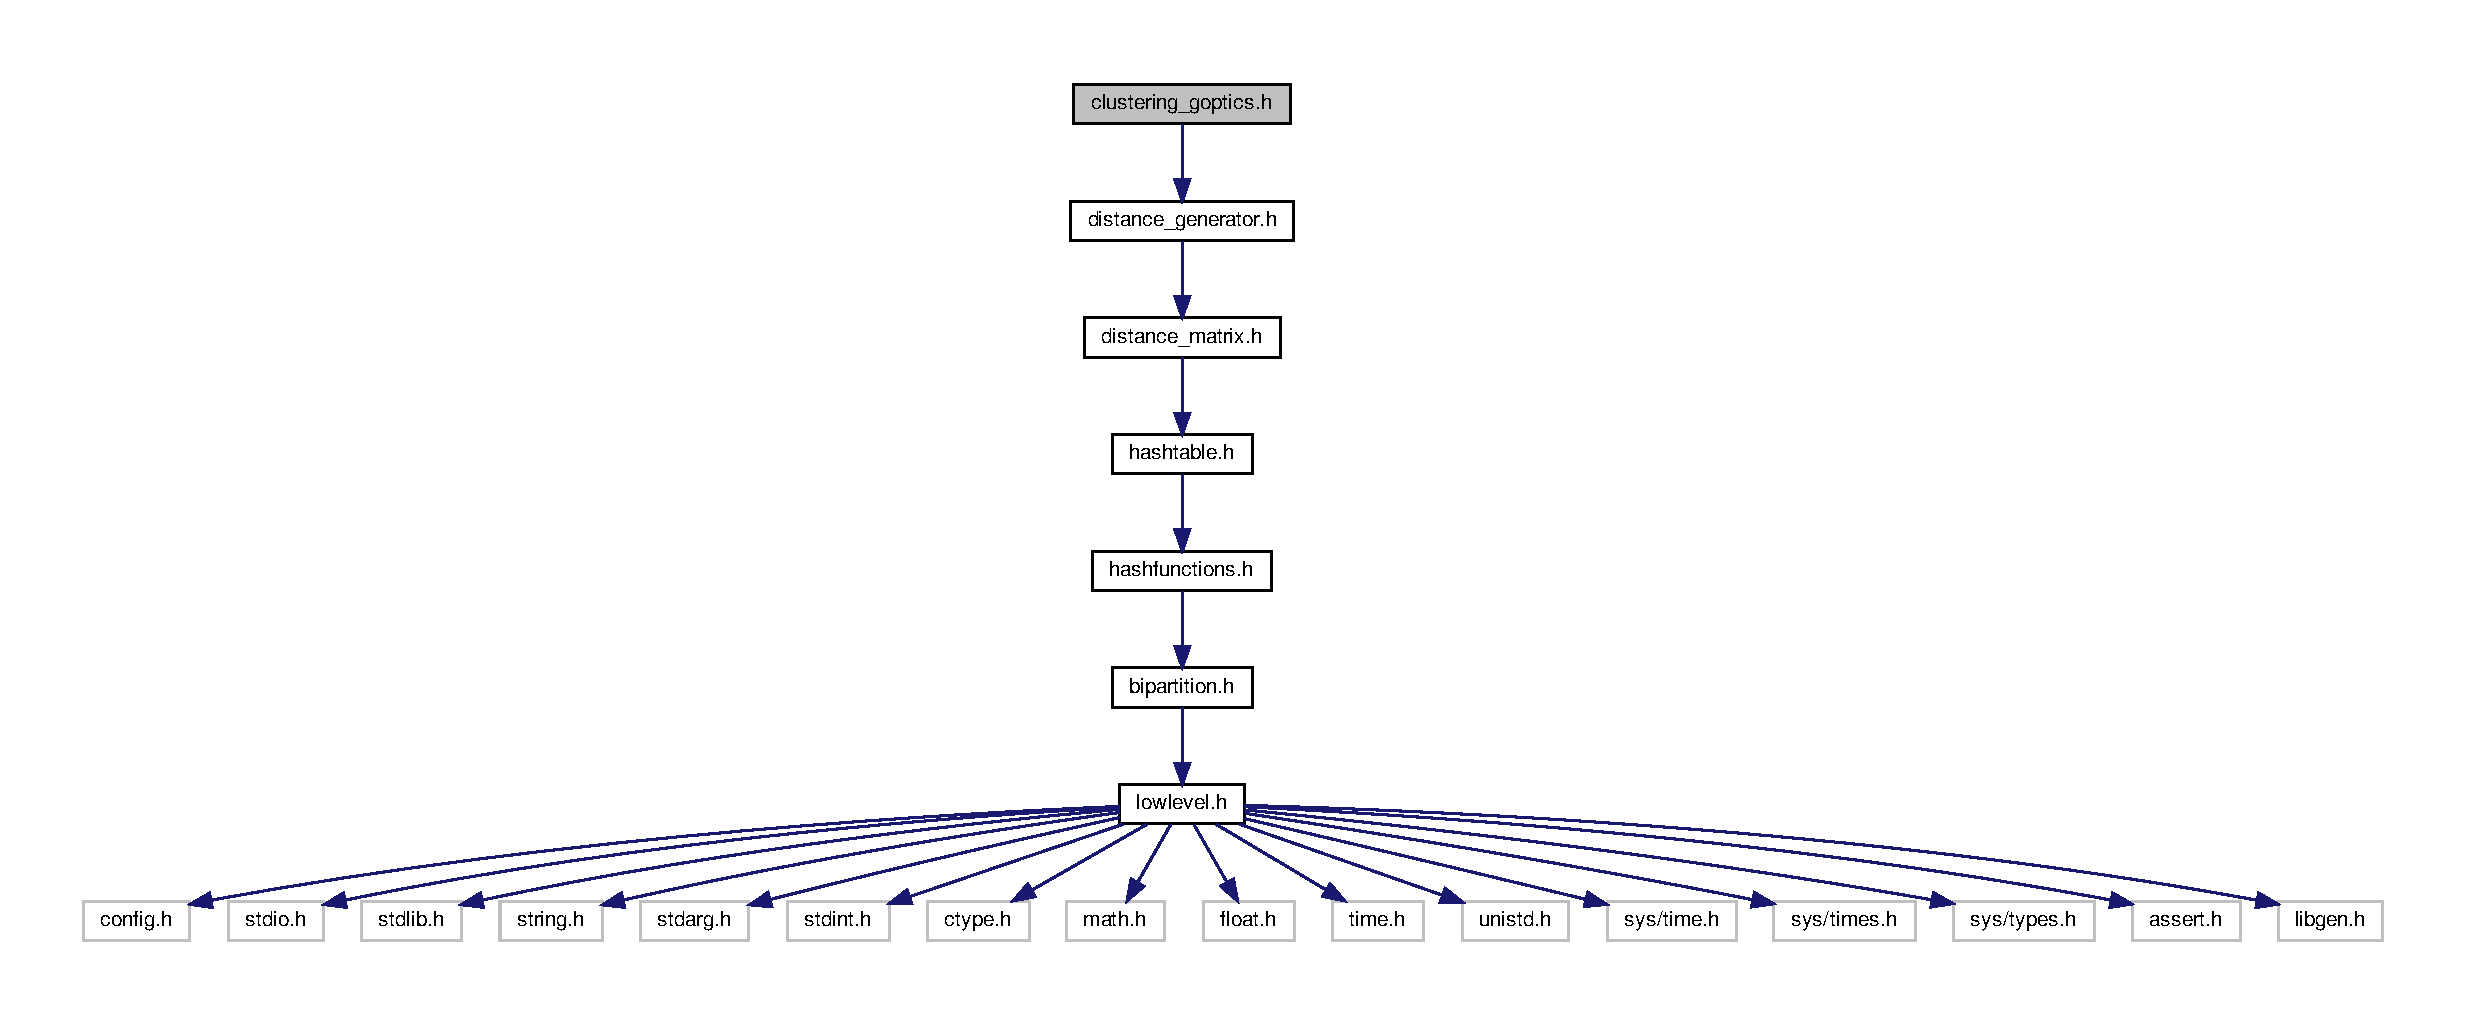
\includegraphics[width=350pt]{clustering__goptics_8h__incl}
\end{center}
\end{figure}
This graph shows which files directly or indirectly include this file\+:\nopagebreak
\begin{figure}[H]
\begin{center}
\leavevmode
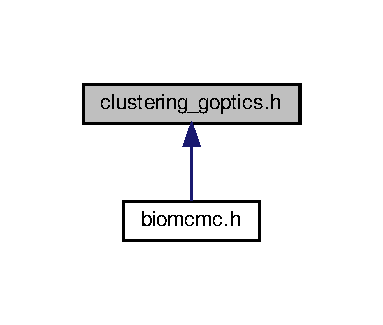
\includegraphics[width=184pt]{clustering__goptics_8h__dep__incl}
\end{center}
\end{figure}
\subsubsection*{Data Structures}
\begin{DoxyCompactItemize}
\item 
struct \hyperlink{structgoptics__cluster__struct}{goptics\+\_\+cluster\+\_\+struct}
\end{DoxyCompactItemize}
\subsubsection*{Typedefs}
\begin{DoxyCompactItemize}
\item 
\mbox{\Hypertarget{clustering__goptics_8h_a2dc42240fd521593576575db239a9ab4}\label{clustering__goptics_8h_a2dc42240fd521593576575db239a9ab4}} 
typedef struct \hyperlink{structgoptics__cluster__struct}{goptics\+\_\+cluster\+\_\+struct} $\ast$ {\bfseries goptics\+\_\+cluster}
\end{DoxyCompactItemize}
\subsubsection*{Functions}
\begin{DoxyCompactItemize}
\item 
\mbox{\Hypertarget{clustering__goptics_8h_a7557f763a43b78acea3f92363440a8ec}\label{clustering__goptics_8h_a7557f763a43b78acea3f92363440a8ec}} 
\hyperlink{structgoptics__cluster__struct}{goptics\+\_\+cluster} {\bfseries new\+\_\+goptics\+\_\+cluster} (\hyperlink{structdistance__generator__struct}{distance\+\_\+generator} dg, int min\+\_\+points, double epsilon)
\item 
\mbox{\Hypertarget{clustering__goptics_8h_a74fd5bce22679ffce1333eeaa27d304a}\label{clustering__goptics_8h_a74fd5bce22679ffce1333eeaa27d304a}} 
\hyperlink{structgoptics__cluster__struct}{goptics\+\_\+cluster} {\bfseries new\+\_\+goptics\+\_\+cluster\+\_\+run} (\hyperlink{structdistance__generator__struct}{distance\+\_\+generator} dg, int min\+\_\+points, double epsilon)
\item 
\mbox{\Hypertarget{clustering__goptics_8h_a05d76232aa2127e922dcfe8cae698454}\label{clustering__goptics_8h_a05d76232aa2127e922dcfe8cae698454}} 
void {\bfseries del\+\_\+goptics\+\_\+cluster} (\hyperlink{structgoptics__cluster__struct}{goptics\+\_\+cluster} gop)
\item 
\mbox{\Hypertarget{clustering__goptics_8h_a46d134c3cf060665a350d0459d14994c}\label{clustering__goptics_8h_a46d134c3cf060665a350d0459d14994c}} 
void {\bfseries assign\+\_\+goptics\+\_\+clusters} (\hyperlink{structgoptics__cluster__struct}{goptics\+\_\+cluster} gop, double cluster\+\_\+eps)
\end{DoxyCompactItemize}


\subsubsection{Detailed Description}
O\+P\+T\+I\+CS algorithm based on \href{https://github.com/guineri/GOPTICS}{\tt https\+://github.\+com/guineri/\+G\+O\+P\+T\+I\+CS}. 


\hypertarget{distance__generator_8h}{}\subsection{distance\+\_\+generator.\+h File Reference}
\label{distance__generator_8h}\index{distance\+\_\+generator.\+h@{distance\+\_\+generator.\+h}}


distance calculation between generic objects,without generating full matrix beforehand  


{\ttfamily \#include \char`\"{}distance\+\_\+matrix.\+h\char`\"{}}\newline
Include dependency graph for distance\+\_\+generator.\+h\+:\nopagebreak
\begin{figure}[H]
\begin{center}
\leavevmode
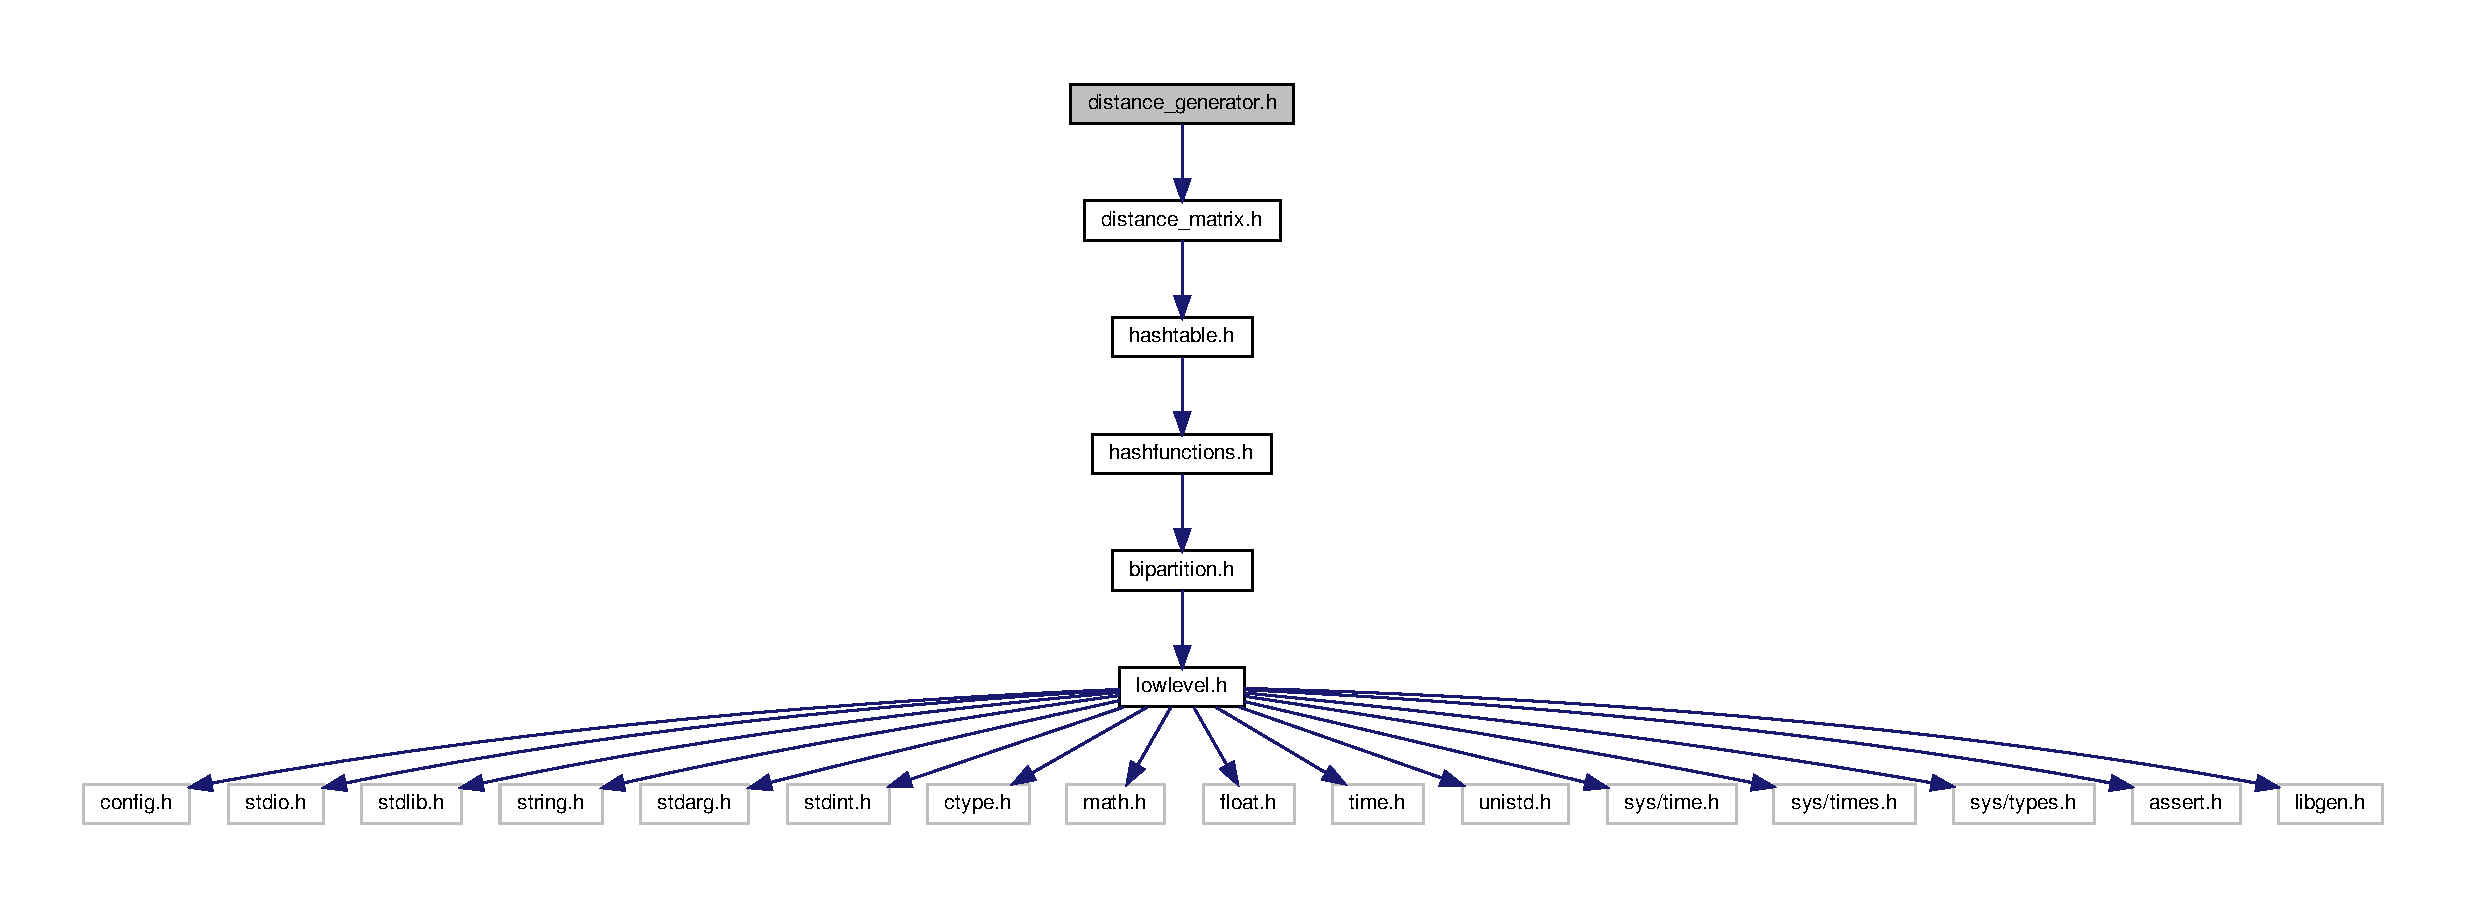
\includegraphics[width=350pt]{distance__generator_8h__incl}
\end{center}
\end{figure}
This graph shows which files directly or indirectly include this file\+:\nopagebreak
\begin{figure}[H]
\begin{center}
\leavevmode
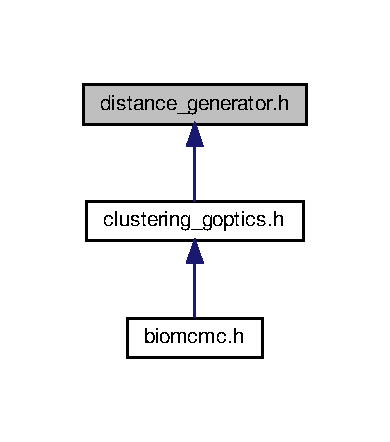
\includegraphics[width=187pt]{distance__generator_8h__dep__incl}
\end{center}
\end{figure}
\subsubsection*{Data Structures}
\begin{DoxyCompactItemize}
\item 
struct \hyperlink{structdistance__generator__struct}{distance\+\_\+generator\+\_\+struct}
\end{DoxyCompactItemize}
\subsubsection*{Typedefs}
\begin{DoxyCompactItemize}
\item 
\mbox{\Hypertarget{distance__generator_8h_a199b15e30dbca7bb6d2f4fb8f7e13f9c}\label{distance__generator_8h_a199b15e30dbca7bb6d2f4fb8f7e13f9c}} 
typedef struct \hyperlink{structdistance__generator__struct}{distance\+\_\+generator\+\_\+struct} $\ast$ {\bfseries distance\+\_\+generator}
\end{DoxyCompactItemize}
\subsubsection*{Functions}
\begin{DoxyCompactItemize}
\item 
\mbox{\Hypertarget{distance__generator_8h_ad908f1218c2e31e549e34a9686f9f408}\label{distance__generator_8h_ad908f1218c2e31e549e34a9686f9f408}} 
\hyperlink{structdistance__generator__struct}{distance\+\_\+generator} {\bfseries new\+\_\+distance\+\_\+generator} (int n\+\_\+samples, int n\+\_\+distances)
\item 
\mbox{\Hypertarget{distance__generator_8h_a70ef842b533194a7ef1334171935e11e}\label{distance__generator_8h_a70ef842b533194a7ef1334171935e11e}} 
void {\bfseries del\+\_\+distance\+\_\+generator} (\hyperlink{structdistance__generator__struct}{distance\+\_\+generator} d)
\item 
\mbox{\Hypertarget{distance__generator_8h_a17475da6b045ddb3f019c30cf9eea89f}\label{distance__generator_8h_a17475da6b045ddb3f019c30cf9eea89f}} 
double {\bfseries distance\+\_\+generator\+\_\+get\+\_\+at\+\_\+distance} (\hyperlink{structdistance__generator__struct}{distance\+\_\+generator} d, int i, int j, int which\+\_\+distance)
\item 
\mbox{\Hypertarget{distance__generator_8h_ae653fc52f2a6a3db63548c484a041385}\label{distance__generator_8h_ae653fc52f2a6a3db63548c484a041385}} 
double {\bfseries distance\+\_\+generator\+\_\+get} (\hyperlink{structdistance__generator__struct}{distance\+\_\+generator} d, int i, int j)
\item 
\mbox{\Hypertarget{distance__generator_8h_a1250f80cf59fde9c5bf20ba467720866}\label{distance__generator_8h_a1250f80cf59fde9c5bf20ba467720866}} 
void \hyperlink{distance__generator_8h_a1250f80cf59fde9c5bf20ba467720866}{distance\+\_\+generator\+\_\+set\+\_\+function\+\_\+data} (\hyperlink{structdistance__generator__struct}{distance\+\_\+generator} d, void($\ast$lowlevel\+\_\+dist\+\_\+funct)(void $\ast$, int, int, double $\ast$), void $\ast$extra\+\_\+data)
\begin{DoxyCompactList}\small\item\em defines distance calculation function wrapper, and all extra data needed by wrapper; no check is done here, but wrapper should return at least as many distances sd n\+\_\+distances (wrapper functions can check) \end{DoxyCompactList}\item 
\mbox{\Hypertarget{distance__generator_8h_afbb17068a9677c5cfac04c8f2b05c99a}\label{distance__generator_8h_afbb17068a9677c5cfac04c8f2b05c99a}} 
void \hyperlink{distance__generator_8h_afbb17068a9677c5cfac04c8f2b05c99a}{distance\+\_\+generator\+\_\+set\+\_\+which\+\_\+distance} (\hyperlink{structdistance__generator__struct}{distance\+\_\+generator} d, int which\+\_\+distance)
\begin{DoxyCompactList}\small\item\em distance wrapper may return several distances, but only one is returned by get(); this sets which one (should be called before e.\+g. clustering) \end{DoxyCompactList}\item 
\mbox{\Hypertarget{distance__generator_8h_acf74f230963e2b57697f93815d1d1ed0}\label{distance__generator_8h_acf74f230963e2b57697f93815d1d1ed0}} 
void {\bfseries distance\+\_\+generator\+\_\+reset} (\hyperlink{structdistance__generator__struct}{distance\+\_\+generator} d)
\end{DoxyCompactItemize}


\subsubsection{Detailed Description}
distance calculation between generic objects,without generating full matrix beforehand 


\hypertarget{distance__matrix_8h}{}\subsection{distance\+\_\+matrix.\+h File Reference}
\label{distance__matrix_8h}\index{distance\+\_\+matrix.\+h@{distance\+\_\+matrix.\+h}}


distance matrix, that can be used in alignments and trees, and patristic-\/distance based species distances  


{\ttfamily \#include \char`\"{}hashtable.\+h\char`\"{}}\newline
Include dependency graph for distance\+\_\+matrix.\+h\+:\nopagebreak
\begin{figure}[H]
\begin{center}
\leavevmode
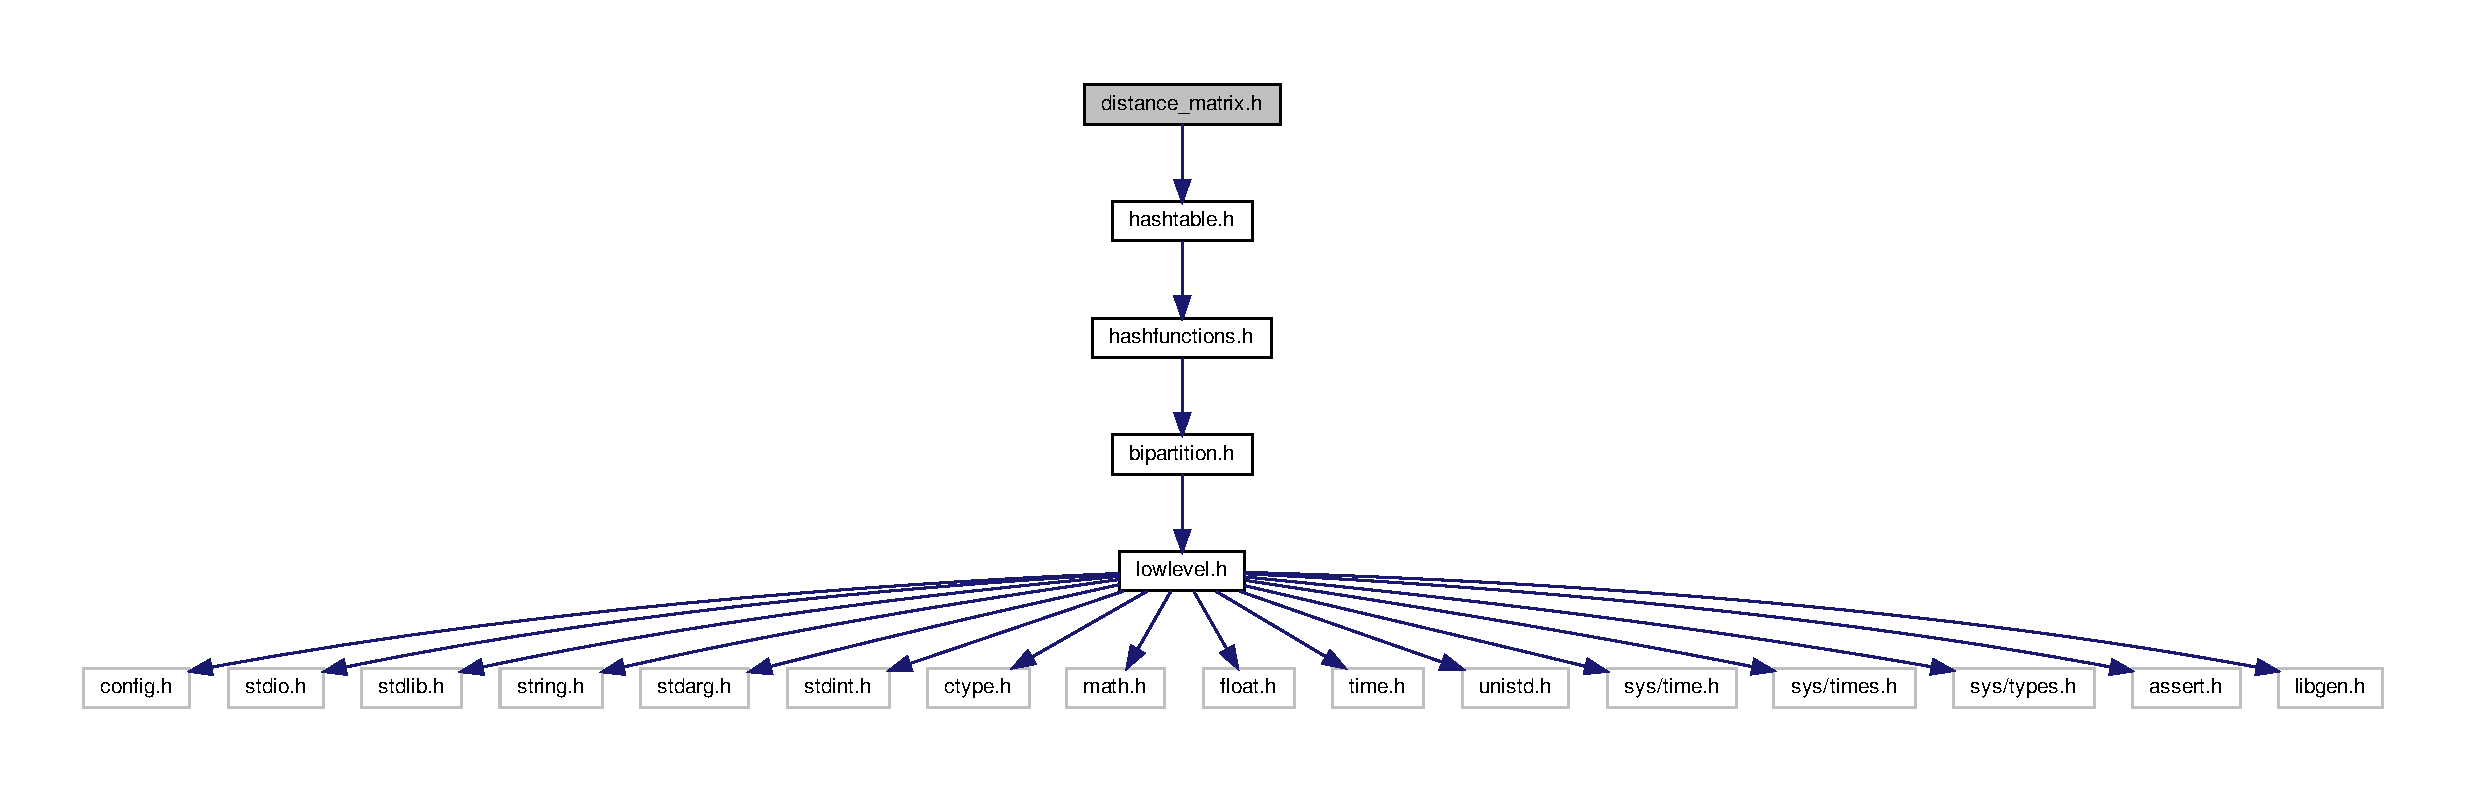
\includegraphics[width=350pt]{distance__matrix_8h__incl}
\end{center}
\end{figure}
This graph shows which files directly or indirectly include this file\+:\nopagebreak
\begin{figure}[H]
\begin{center}
\leavevmode
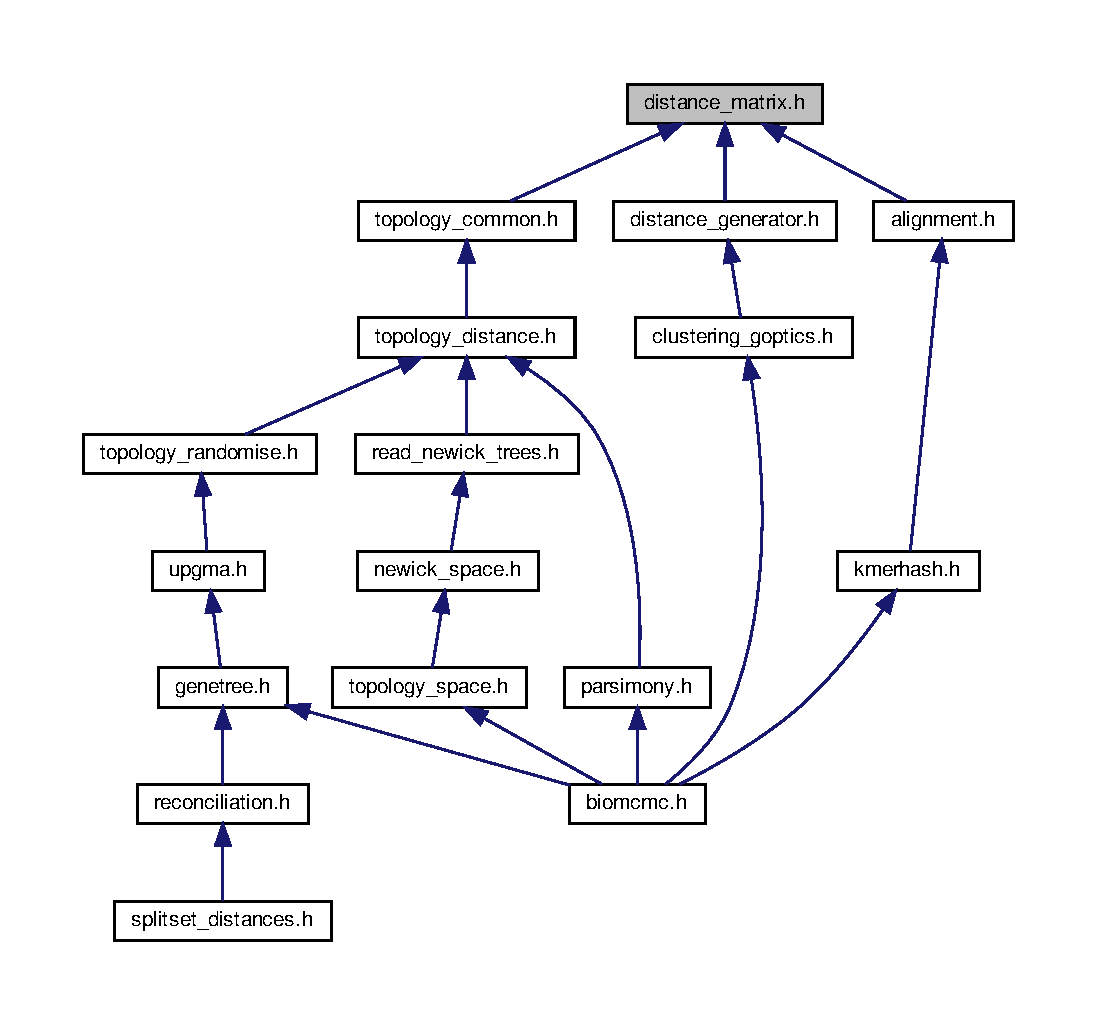
\includegraphics[width=350pt]{distance__matrix_8h__dep__incl}
\end{center}
\end{figure}
\subsubsection*{Data Structures}
\begin{DoxyCompactItemize}
\item 
struct \hyperlink{structdistance__matrix__struct}{distance\+\_\+matrix\+\_\+struct}
\item 
struct \hyperlink{structspdist__matrix__struct}{spdist\+\_\+matrix\+\_\+struct}
\end{DoxyCompactItemize}
\subsubsection*{Typedefs}
\begin{DoxyCompactItemize}
\item 
\mbox{\Hypertarget{distance__matrix_8h_a9e145719317f4d9e5067479ec7d53bb8}\label{distance__matrix_8h_a9e145719317f4d9e5067479ec7d53bb8}} 
typedef struct \hyperlink{structdistance__matrix__struct}{distance\+\_\+matrix\+\_\+struct} $\ast$ {\bfseries distance\+\_\+matrix}
\item 
\mbox{\Hypertarget{distance__matrix_8h_ad771eef7a2693d94a03fb0b80df60664}\label{distance__matrix_8h_ad771eef7a2693d94a03fb0b80df60664}} 
typedef struct \hyperlink{structspdist__matrix__struct}{spdist\+\_\+matrix\+\_\+struct} $\ast$ {\bfseries spdist\+\_\+matrix}
\end{DoxyCompactItemize}
\subsubsection*{Functions}
\begin{DoxyCompactItemize}
\item 
\mbox{\Hypertarget{distance__matrix_8h_a05c728b75adbababd8c6fd4de241912a}\label{distance__matrix_8h_a05c728b75adbababd8c6fd4de241912a}} 
\hyperlink{structdistance__matrix__struct}{distance\+\_\+matrix} \hyperlink{distance__matrix_8h_a05c728b75adbababd8c6fd4de241912a}{new\+\_\+distance\+\_\+matrix} (int nseqs)
\begin{DoxyCompactList}\small\item\em creates new matrix of pairwise distances \end{DoxyCompactList}\item 
\mbox{\Hypertarget{distance__matrix_8h_a32656dd2ef988382d7e7a3eb505d1522}\label{distance__matrix_8h_a32656dd2ef988382d7e7a3eb505d1522}} 
void \hyperlink{distance__matrix_8h_a32656dd2ef988382d7e7a3eb505d1522}{zero\+\_\+lower\+\_\+distance\+\_\+matrix} (\hyperlink{structdistance__matrix__struct}{distance\+\_\+matrix} dist)
\begin{DoxyCompactList}\small\item\em specially in gene/sptree distance methods (G\+L\+A\+SS, S\+T\+E\+AC, etc.) lower is used for means and upper for min. This function resets matrix elements \end{DoxyCompactList}\item 
\mbox{\Hypertarget{distance__matrix_8h_a5ac533926151f08c78923a645ab11446}\label{distance__matrix_8h_a5ac533926151f08c78923a645ab11446}} 
void \hyperlink{distance__matrix_8h_a5ac533926151f08c78923a645ab11446}{transpose\+\_\+distance\+\_\+matrix} (\hyperlink{structdistance__matrix__struct}{distance\+\_\+matrix} dist)
\begin{DoxyCompactList}\small\item\em invert lower and upper diagonals of matrix (since some functions like upgma expect upper, etc.) \end{DoxyCompactList}\item 
\mbox{\Hypertarget{distance__matrix_8h_a6c66792124e982cdb5202e1be10c24cf}\label{distance__matrix_8h_a6c66792124e982cdb5202e1be10c24cf}} 
void \hyperlink{distance__matrix_8h_a6c66792124e982cdb5202e1be10c24cf}{del\+\_\+distance\+\_\+matrix} (\hyperlink{structdistance__matrix__struct}{distance\+\_\+matrix} dist)
\begin{DoxyCompactList}\small\item\em releases memory allocated to distance\+\_\+matrix (this structure has no smart ref\+\_\+counter) \end{DoxyCompactList}\item 
\mbox{\Hypertarget{distance__matrix_8h_a9837e1b9bded4fd9e565e714713c390c}\label{distance__matrix_8h_a9837e1b9bded4fd9e565e714713c390c}} 
\hyperlink{structspdist__matrix__struct}{spdist\+\_\+matrix} {\bfseries new\+\_\+spdist\+\_\+matrix} (int n\+\_\+species)
\item 
void \hyperlink{distance__matrix_8h_ae266042e13a382a1890a6fbff681b9f2}{zero\+\_\+all\+\_\+spdist\+\_\+matrix} (\hyperlink{structspdist__matrix__struct}{spdist\+\_\+matrix} dist)
\item 
\mbox{\Hypertarget{distance__matrix_8h_a2be42a346c2a1ba84b8e5694e7eb9893}\label{distance__matrix_8h_a2be42a346c2a1ba84b8e5694e7eb9893}} 
void {\bfseries finalise\+\_\+spdist\+\_\+matrix} (\hyperlink{structspdist__matrix__struct}{spdist\+\_\+matrix} dist)
\item 
\mbox{\Hypertarget{distance__matrix_8h_a6ddbc5097dbe689d2c74ea5fbb56e173}\label{distance__matrix_8h_a6ddbc5097dbe689d2c74ea5fbb56e173}} 
void {\bfseries finalise\+\_\+spdist\+\_\+matrix\+\_\+with\+\_\+rescaling} (\hyperlink{structspdist__matrix__struct}{spdist\+\_\+matrix} dist, double scale)
\item 
\mbox{\Hypertarget{distance__matrix_8h_a3b0ce1bc6fc8e338ca04435fe22b4459}\label{distance__matrix_8h_a3b0ce1bc6fc8e338ca04435fe22b4459}} 
void {\bfseries complete\+\_\+missing\+\_\+spdist\+\_\+from\+\_\+global\+\_\+spdist} (\hyperlink{structspdist__matrix__struct}{spdist\+\_\+matrix} local, \hyperlink{structspdist__matrix__struct}{spdist\+\_\+matrix} global)
\item 
\mbox{\Hypertarget{distance__matrix_8h_ad8672a57540a96d4437a05a775282abe}\label{distance__matrix_8h_ad8672a57540a96d4437a05a775282abe}} 
void {\bfseries copy\+\_\+spdist\+\_\+matrix\+\_\+to\+\_\+distance\+\_\+matrix\+\_\+upper} (\hyperlink{structspdist__matrix__struct}{spdist\+\_\+matrix} spd, \hyperlink{structdistance__matrix__struct}{distance\+\_\+matrix} dist, \hyperlink{lowlevel_8h_a97a80ca1602ebf2303258971a2c938e2}{bool} use\+\_\+means)
\item 
\mbox{\Hypertarget{distance__matrix_8h_a15093d39f1c6485ce09e1a7643ce6736}\label{distance__matrix_8h_a15093d39f1c6485ce09e1a7643ce6736}} 
void {\bfseries del\+\_\+spdist\+\_\+matrix} (\hyperlink{structspdist__matrix__struct}{spdist\+\_\+matrix} dist)
\item 
\mbox{\Hypertarget{distance__matrix_8h_ad04d393e906484301674610590ae2dfe}\label{distance__matrix_8h_ad04d393e906484301674610590ae2dfe}} 
void \hyperlink{distance__matrix_8h_ad04d393e906484301674610590ae2dfe}{fill\+\_\+species\+\_\+dists\+\_\+from\+\_\+gene\+\_\+dists} (\hyperlink{structdistance__matrix__struct}{distance\+\_\+matrix} spdist, \hyperlink{structdistance__matrix__struct}{distance\+\_\+matrix} gendist, int $\ast$sp\+\_\+id, \hyperlink{lowlevel_8h_a97a80ca1602ebf2303258971a2c938e2}{bool} use\+\_\+upper\+\_\+gene)
\begin{DoxyCompactList}\small\item\em updates distances between species based on genes and gene-\/to-\/species mapping, with min on upper and mean on lower diagonal \end{DoxyCompactList}\item 
\mbox{\Hypertarget{distance__matrix_8h_ab5c7f9dfd23d5fab609c82e86a9a7f3d}\label{distance__matrix_8h_ab5c7f9dfd23d5fab609c82e86a9a7f3d}} 
void \hyperlink{distance__matrix_8h_ab5c7f9dfd23d5fab609c82e86a9a7f3d}{update\+\_\+species\+\_\+dists\+\_\+from\+\_\+spdist} (\hyperlink{structdistance__matrix__struct}{distance\+\_\+matrix} global, \hyperlink{structdistance__matrix__struct}{distance\+\_\+matrix} local, int $\ast$spexist)
\begin{DoxyCompactList}\small\item\em update global (over loci) species distances besed on local (within locus) species distances \end{DoxyCompactList}\item 
\mbox{\Hypertarget{distance__matrix_8h_a3302aeae38b037be76a360a5fb8d7898}\label{distance__matrix_8h_a3302aeae38b037be76a360a5fb8d7898}} 
int {\bfseries prepare\+\_\+spdistmatrix\+\_\+from\+\_\+gene\+\_\+species\+\_\+map} (\hyperlink{structspdist__matrix__struct}{spdist\+\_\+matrix} spdist, int $\ast$sp\+\_\+id, int n\+\_\+sp\+\_\+id)
\item 
\mbox{\Hypertarget{distance__matrix_8h_a760f76e6dd06a82994c45dda3d450f37}\label{distance__matrix_8h_a760f76e6dd06a82994c45dda3d450f37}} 
void {\bfseries fill\+\_\+spdistmatrix\+\_\+from\+\_\+gene\+\_\+dists} (\hyperlink{structspdist__matrix__struct}{spdist\+\_\+matrix} spdist, \hyperlink{structdistance__matrix__struct}{distance\+\_\+matrix} gendist, int $\ast$sp\+\_\+id, \hyperlink{lowlevel_8h_a97a80ca1602ebf2303258971a2c938e2}{bool} use\+\_\+upper\+\_\+gene)
\item 
\mbox{\Hypertarget{distance__matrix_8h_ac0bd82593abed577a8be45076f9697c6}\label{distance__matrix_8h_ac0bd82593abed577a8be45076f9697c6}} 
void \hyperlink{distance__matrix_8h_ac0bd82593abed577a8be45076f9697c6}{fill\+\_\+spdistmatrix\+\_\+from\+\_\+gene\+\_\+dist\+\_\+vector} (\hyperlink{structspdist__matrix__struct}{spdist\+\_\+matrix} spdist, double $\ast$gdist, int n\+\_\+gdist, int $\ast$sp\+\_\+id)
\begin{DoxyCompactList}\small\item\em initialise spdist\+\_\+matrix with patristic distances from gdist vector of size n\+\_\+gdist (1D) \end{DoxyCompactList}\item 
\mbox{\Hypertarget{distance__matrix_8h_a4610b2cfcc845942ae75c6f00e4d6bc5}\label{distance__matrix_8h_a4610b2cfcc845942ae75c6f00e4d6bc5}} 
void {\bfseries update\+\_\+spdistmatrix\+\_\+from\+\_\+spdistmatrix} (\hyperlink{structspdist__matrix__struct}{spdist\+\_\+matrix} global, \hyperlink{structspdist__matrix__struct}{spdist\+\_\+matrix} local)
\end{DoxyCompactItemize}


\subsubsection{Detailed Description}
distance matrix, that can be used in alignments and trees, and patristic-\/distance based species distances 

These functions don\textquotesingle{}t know about trees/topologies\+: topology\+\_\+common.\+c creates the actual patristic distances, and downstream software or \hyperlink{genetree_8h}{genetree.\+h} should decide how to use this information 

\subsubsection{Function Documentation}
\mbox{\Hypertarget{distance__matrix_8h_ae266042e13a382a1890a6fbff681b9f2}\label{distance__matrix_8h_ae266042e13a382a1890a6fbff681b9f2}} 
\index{distance\+\_\+matrix.\+h@{distance\+\_\+matrix.\+h}!zero\+\_\+all\+\_\+spdist\+\_\+matrix@{zero\+\_\+all\+\_\+spdist\+\_\+matrix}}
\index{zero\+\_\+all\+\_\+spdist\+\_\+matrix@{zero\+\_\+all\+\_\+spdist\+\_\+matrix}!distance\+\_\+matrix.\+h@{distance\+\_\+matrix.\+h}}
\paragraph{\texorpdfstring{zero\+\_\+all\+\_\+spdist\+\_\+matrix()}{zero\_all\_spdist\_matrix()}}
{\footnotesize\ttfamily void zero\+\_\+all\+\_\+spdist\+\_\+matrix (\begin{DoxyParamCaption}\item[{\hyperlink{structspdist__matrix__struct}{spdist\+\_\+matrix}}]{dist }\end{DoxyParamCaption})}

zero both mean\mbox{[}\mbox{]} and min\mbox{[}\mbox{]} since we only look at average (never min) across loci 
\hypertarget{empirical__frequency_8c}{}\subsection{empirical\+\_\+frequency.\+c File Reference}
\label{empirical__frequency_8c}\index{empirical\+\_\+frequency.\+c@{empirical\+\_\+frequency.\+c}}


histogram of vectors, ordered by frequency. Also calculates M\+AP (modal) values.  


{\ttfamily \#include \char`\"{}empirical\+\_\+frequency.\+h\char`\"{}}\newline
Include dependency graph for empirical\+\_\+frequency.\+c\+:\nopagebreak
\begin{figure}[H]
\begin{center}
\leavevmode
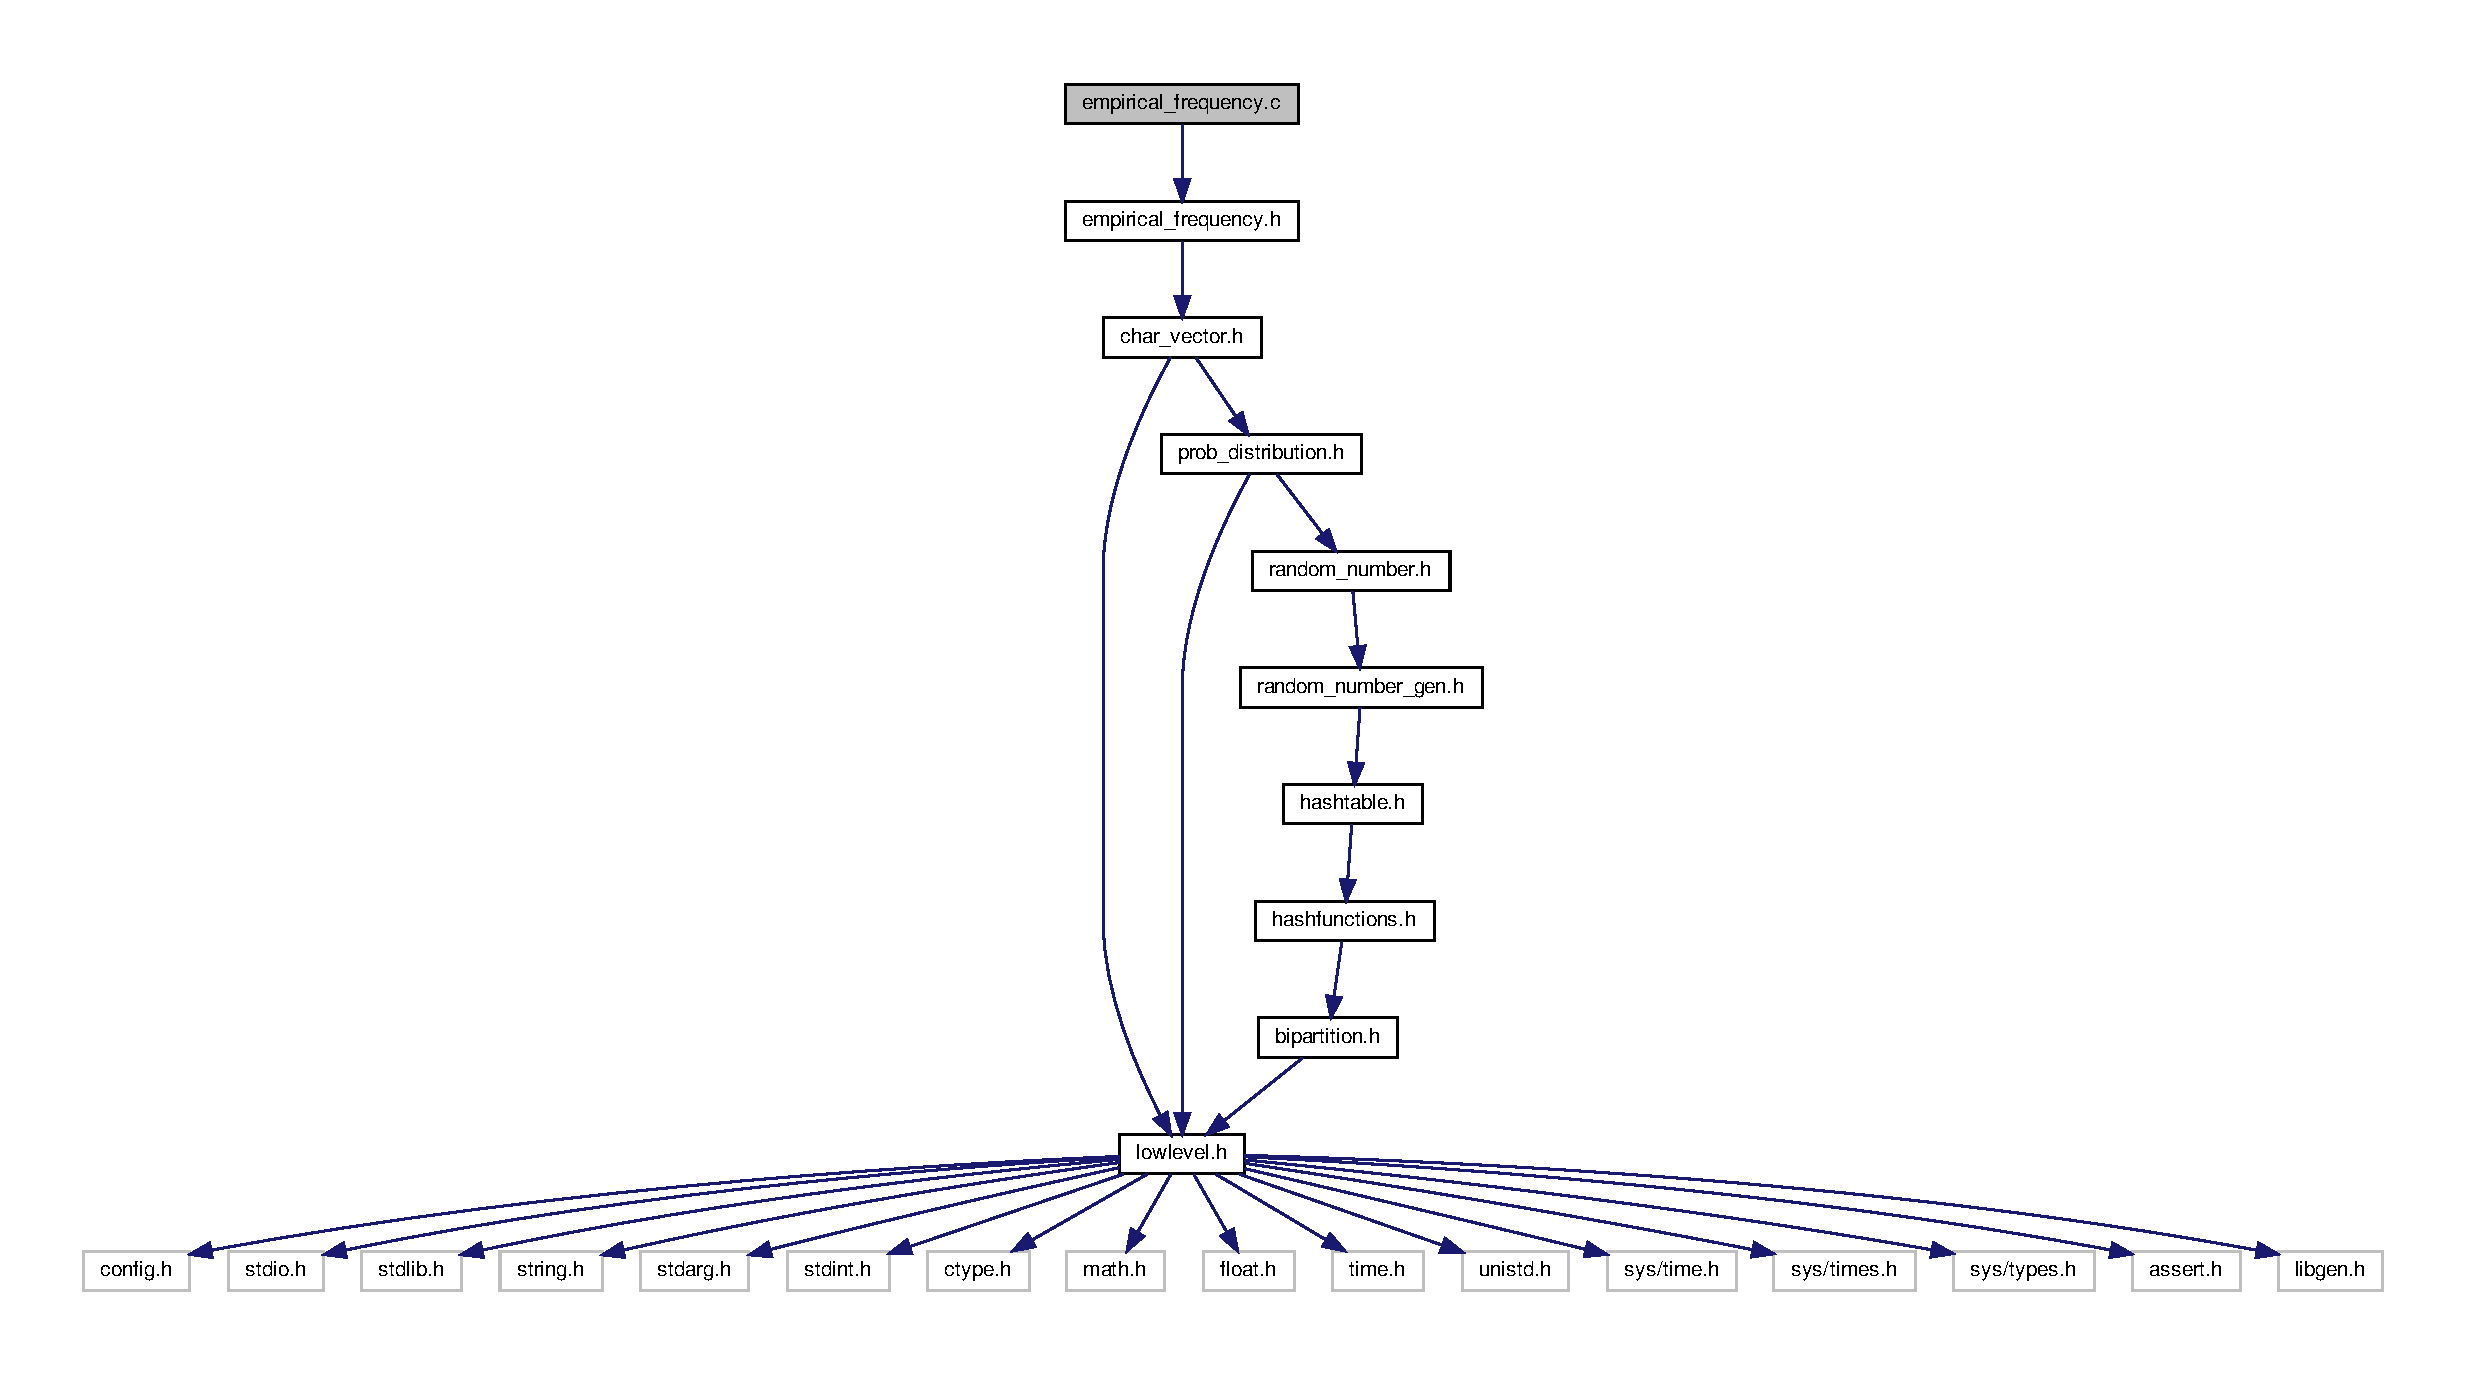
\includegraphics[width=350pt]{empirical__frequency_8c__incl}
\end{center}
\end{figure}
\subsubsection*{Functions}
\begin{DoxyCompactItemize}
\item 
\mbox{\Hypertarget{empirical__frequency_8c_a20f41f75f452430f54bce9309a093634}\label{empirical__frequency_8c_a20f41f75f452430f54bce9309a093634}} 
int {\bfseries compare\+\_\+empfreq\+\_\+element\+\_\+decreasing} (const void $\ast$a, const void $\ast$b)
\item 
\mbox{\Hypertarget{empirical__frequency_8c_ae30bc9e64d459dc191ec42bc00f8c9e2}\label{empirical__frequency_8c_ae30bc9e64d459dc191ec42bc00f8c9e2}} 
int {\bfseries compare\+\_\+empfreq\+\_\+element\+\_\+increasing} (const void $\ast$a, const void $\ast$b)
\item 
\mbox{\Hypertarget{empirical__frequency_8c_a4cd418a2c4ef058c53bf98e3b4a1e3f0}\label{empirical__frequency_8c_a4cd418a2c4ef058c53bf98e3b4a1e3f0}} 
int {\bfseries compare\+\_\+empfreq\+\_\+double\+\_\+element\+\_\+decreasing} (const void $\ast$a, const void $\ast$b)
\item 
\mbox{\Hypertarget{empirical__frequency_8c_ae44d217dc4fff8b1aecb319f6cb01267}\label{empirical__frequency_8c_ae44d217dc4fff8b1aecb319f6cb01267}} 
int {\bfseries compare\+\_\+empfreq\+\_\+double\+\_\+element\+\_\+increasing} (const void $\ast$a, const void $\ast$b)
\item 
\mbox{\Hypertarget{empirical__frequency_8c_a146554a6d5fea1f46a55b1ae55c0d3ab}\label{empirical__frequency_8c_a146554a6d5fea1f46a55b1ae55c0d3ab}} 
\hyperlink{structempfreq__struct}{empfreq} {\bfseries create\+\_\+empfreq\+\_\+from\+\_\+value\+\_\+sorted\+\_\+empfreq} (\hyperlink{structempfreq__struct}{empfreq} e\+\_\+idx)
\item 
\mbox{\Hypertarget{empirical__frequency_8c_a883436dac9e99833cab9d62a553e3393}\label{empirical__frequency_8c_a883436dac9e99833cab9d62a553e3393}} 
void {\bfseries sort\+\_\+empfreq\+\_\+decreasing} (\hyperlink{structempfreq__struct}{empfreq} ef)
\item 
\mbox{\Hypertarget{empirical__frequency_8c_a4ca795838c0d6e8c921f41d04d72e7e7}\label{empirical__frequency_8c_a4ca795838c0d6e8c921f41d04d72e7e7}} 
void {\bfseries sort\+\_\+empfreq\+\_\+increasing} (\hyperlink{structempfreq__struct}{empfreq} ef)
\item 
\mbox{\Hypertarget{empirical__frequency_8c_ad796ad27f50c6a0de9076ba99bc1389c}\label{empirical__frequency_8c_ad796ad27f50c6a0de9076ba99bc1389c}} 
void {\bfseries sort\+\_\+empfreq\+\_\+double\+\_\+decreasing} (\hyperlink{structempfreq__double__struct}{empfreq\+\_\+double} efd)
\item 
\mbox{\Hypertarget{empirical__frequency_8c_a2baf312f7e3310e2c34add4174a38e61}\label{empirical__frequency_8c_a2baf312f7e3310e2c34add4174a38e61}} 
void {\bfseries sort\+\_\+empfreq\+\_\+double\+\_\+increasing} (\hyperlink{structempfreq__double__struct}{empfreq\+\_\+double} efd)
\item 
\mbox{\Hypertarget{empirical__frequency_8c_af29ae63dc2ba0e09a3ef17074ecc3722}\label{empirical__frequency_8c_af29ae63dc2ba0e09a3ef17074ecc3722}} 
\hyperlink{structempfreq__struct}{empfreq} {\bfseries new\+\_\+empfreq} (int n\+\_\+elements)
\item 
\mbox{\Hypertarget{empirical__frequency_8c_ab200afda862e45c81973c357d90f5c79}\label{empirical__frequency_8c_ab200afda862e45c81973c357d90f5c79}} 
void {\bfseries del\+\_\+empfreq} (\hyperlink{structempfreq__struct}{empfreq} ef)
\item 
\mbox{\Hypertarget{empirical__frequency_8c_a6979f32cf3c75655f5d5986d4a3154cb}\label{empirical__frequency_8c_a6979f32cf3c75655f5d5986d4a3154cb}} 
\hyperlink{structempfreq__double__struct}{empfreq\+\_\+double} {\bfseries new\+\_\+empfreq\+\_\+double} (int n\+\_\+elements)
\item 
\mbox{\Hypertarget{empirical__frequency_8c_a42542f31ac601f146512cf3db771ee19}\label{empirical__frequency_8c_a42542f31ac601f146512cf3db771ee19}} 
void {\bfseries del\+\_\+empfreq\+\_\+double} (\hyperlink{structempfreq__double__struct}{empfreq\+\_\+double} efd)
\item 
\mbox{\Hypertarget{empirical__frequency_8c_a5a2b2680c5665f5dbbba4203a3b2cccc}\label{empirical__frequency_8c_a5a2b2680c5665f5dbbba4203a3b2cccc}} 
\hyperlink{structempfreq__struct}{empfreq} {\bfseries new\+\_\+empfreq\+\_\+sort\+\_\+decreasing} (void $\ast$vec, int n, char type)
\item 
\mbox{\Hypertarget{empirical__frequency_8c_a439290b518a52dfeeacb2181098471b5}\label{empirical__frequency_8c_a439290b518a52dfeeacb2181098471b5}} 
\hyperlink{structempfreq__struct}{empfreq} {\bfseries new\+\_\+empfreq\+\_\+sort\+\_\+increasing} (void $\ast$vec, int n, char type)
\item 
\mbox{\Hypertarget{empirical__frequency_8c_a31c8b778edaf42c8e45167a3bd9224a2}\label{empirical__frequency_8c_a31c8b778edaf42c8e45167a3bd9224a2}} 
\hyperlink{structempfreq__double__struct}{empfreq\+\_\+double} {\bfseries new\+\_\+empfreq\+\_\+double\+\_\+sort\+\_\+decreasing} (double $\ast$vec, int n)
\item 
\mbox{\Hypertarget{empirical__frequency_8c_a65e22155e4908fd77debc350433548a8}\label{empirical__frequency_8c_a65e22155e4908fd77debc350433548a8}} 
\hyperlink{structempfreq__double__struct}{empfreq\+\_\+double} {\bfseries new\+\_\+empfreq\+\_\+double\+\_\+sort\+\_\+increasing} (double $\ast$vec, int n)
\item 
\mbox{\Hypertarget{empirical__frequency_8c_a5b18bcddcbbc46533f9b8bb9346449f5}\label{empirical__frequency_8c_a5b18bcddcbbc46533f9b8bb9346449f5}} 
\hyperlink{structempfreq__struct}{empfreq} {\bfseries new\+\_\+empfreq\+\_\+from\+\_\+int} (int $\ast$vec, int n)
\item 
\mbox{\Hypertarget{empirical__frequency_8c_a47713095e0b7efcba35914b682235779}\label{empirical__frequency_8c_a47713095e0b7efcba35914b682235779}} 
\hyperlink{structempfreq__struct}{empfreq} {\bfseries new\+\_\+empfreq\+\_\+from\+\_\+int\+\_\+weighted} (int $\ast$vec, int n, int $\ast$weight)
\item 
\mbox{\Hypertarget{empirical__frequency_8c_a93113277b6c277f54dff4538fcf1a3cd}\label{empirical__frequency_8c_a93113277b6c277f54dff4538fcf1a3cd}} 
int {\bfseries find\+\_\+mode\+\_\+int} (int $\ast$vec, int n)
\item 
\mbox{\Hypertarget{empirical__frequency_8c_a67c385d014f62ac7b7dd4cd34ae04dd0}\label{empirical__frequency_8c_a67c385d014f62ac7b7dd4cd34ae04dd0}} 
int {\bfseries find\+\_\+mode\+\_\+int\+\_\+weighted} (int $\ast$vec, int n, int $\ast$weight)
\end{DoxyCompactItemize}


\subsubsection{Detailed Description}
histogram of vectors, ordered by frequency. Also calculates M\+AP (modal) values. 

Sorts a vector of integers by their frequencies, preserving their original indexes. It is a simple extension to qsort where the original order can be reconstructed, or still a key/value sorting. 
\hypertarget{empirical__frequency_8h}{}\subsection{empirical\+\_\+frequency.\+h File Reference}
\label{empirical__frequency_8h}\index{empirical\+\_\+frequency.\+h@{empirical\+\_\+frequency.\+h}}


Creates a histogram of a vector, ordered by frequency.  


{\ttfamily \#include \char`\"{}char\+\_\+vector.\+h\char`\"{}}\newline
Include dependency graph for empirical\+\_\+frequency.\+h\+:\nopagebreak
\begin{figure}[H]
\begin{center}
\leavevmode
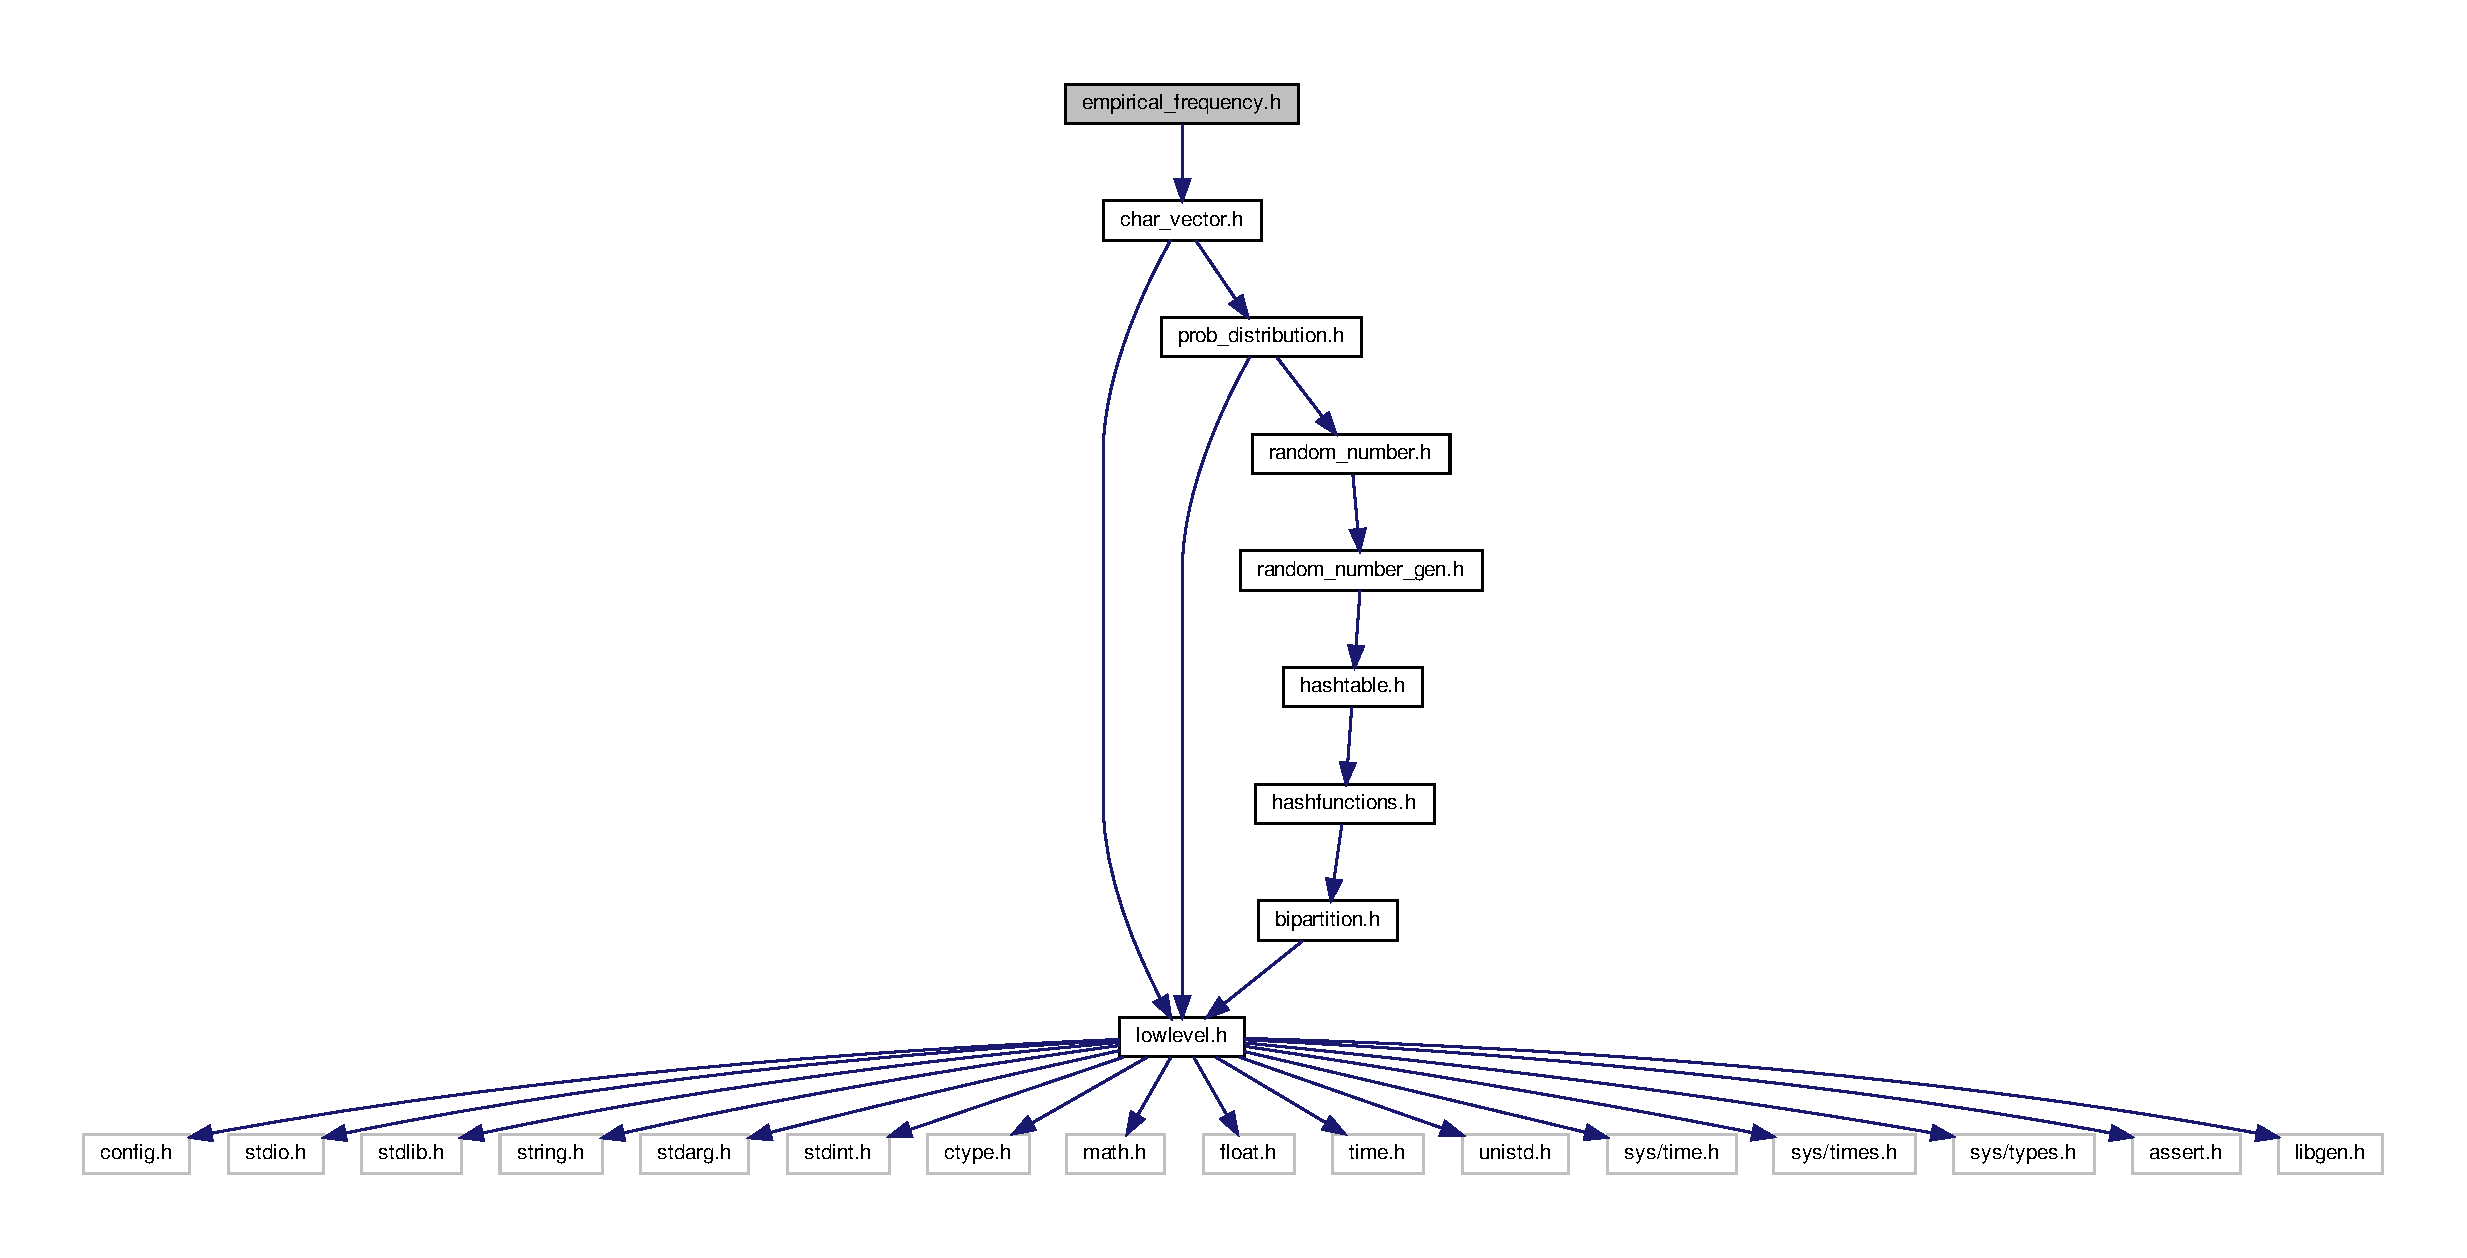
\includegraphics[width=350pt]{empirical__frequency_8h__incl}
\end{center}
\end{figure}
This graph shows which files directly or indirectly include this file\+:\nopagebreak
\begin{figure}[H]
\begin{center}
\leavevmode
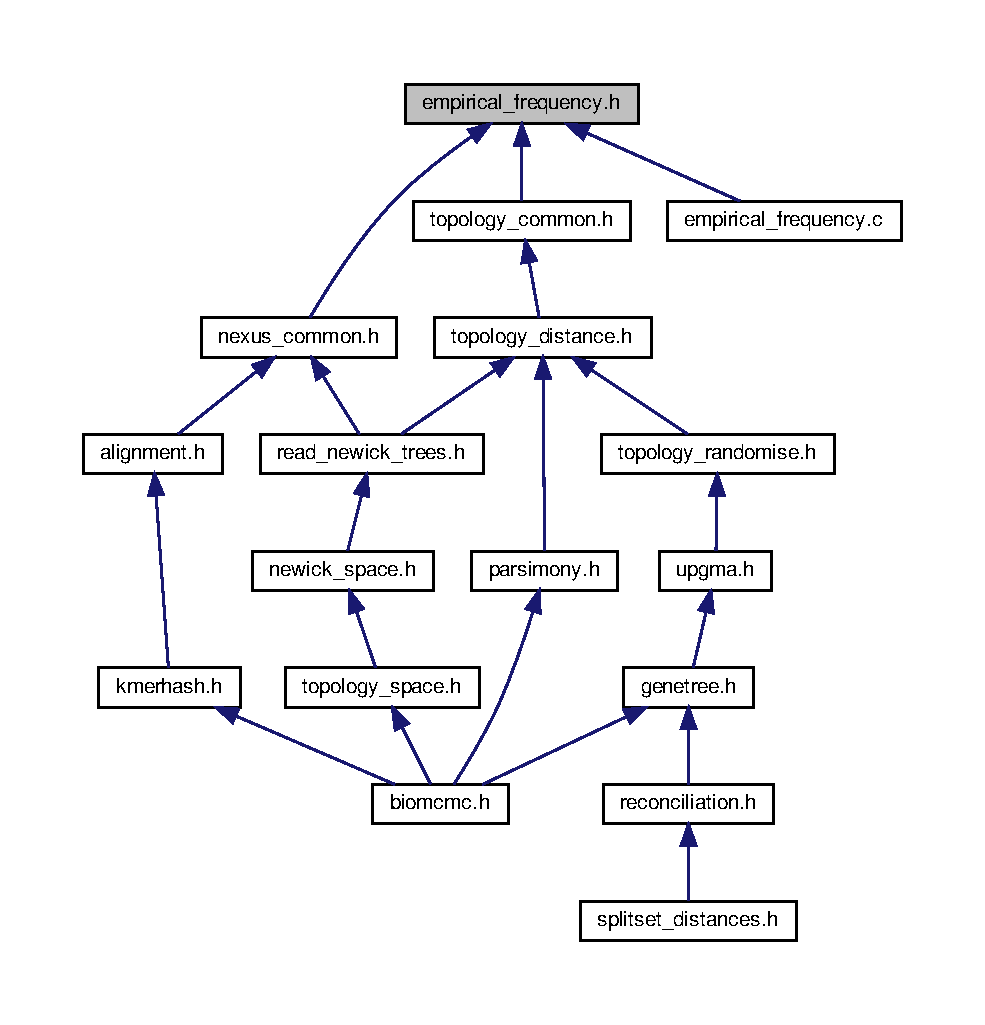
\includegraphics[width=350pt]{empirical__frequency_8h__dep__incl}
\end{center}
\end{figure}
\subsubsection*{Data Structures}
\begin{DoxyCompactItemize}
\item 
struct \hyperlink{structempfreq__element}{empfreq\+\_\+element}
\item 
struct \hyperlink{structempfreq__double__element}{empfreq\+\_\+double\+\_\+element}
\item 
struct \hyperlink{structempfreq__struct}{empfreq\+\_\+struct}
\item 
struct \hyperlink{structempfreq__double__struct}{empfreq\+\_\+double\+\_\+struct}
\end{DoxyCompactItemize}
\subsubsection*{Typedefs}
\begin{DoxyCompactItemize}
\item 
\mbox{\Hypertarget{empirical__frequency_8h_a34df158c1b2c356bd28d4869cc218c9f}\label{empirical__frequency_8h_a34df158c1b2c356bd28d4869cc218c9f}} 
typedef struct \hyperlink{structempfreq__struct}{empfreq\+\_\+struct} $\ast$ {\bfseries empfreq}
\item 
\mbox{\Hypertarget{empirical__frequency_8h_ad6b13ee850747205ac61777a7f331434}\label{empirical__frequency_8h_ad6b13ee850747205ac61777a7f331434}} 
typedef struct \hyperlink{structempfreq__double__struct}{empfreq\+\_\+double\+\_\+struct} $\ast$ {\bfseries empfreq\+\_\+double}
\end{DoxyCompactItemize}
\subsubsection*{Functions}
\begin{DoxyCompactItemize}
\item 
\mbox{\Hypertarget{empirical__frequency_8h_a883436dac9e99833cab9d62a553e3393}\label{empirical__frequency_8h_a883436dac9e99833cab9d62a553e3393}} 
void {\bfseries sort\+\_\+empfreq\+\_\+decreasing} (\hyperlink{structempfreq__struct}{empfreq} ef)
\item 
\mbox{\Hypertarget{empirical__frequency_8h_a4ca795838c0d6e8c921f41d04d72e7e7}\label{empirical__frequency_8h_a4ca795838c0d6e8c921f41d04d72e7e7}} 
void {\bfseries sort\+\_\+empfreq\+\_\+increasing} (\hyperlink{structempfreq__struct}{empfreq} ef)
\item 
\mbox{\Hypertarget{empirical__frequency_8h_ad796ad27f50c6a0de9076ba99bc1389c}\label{empirical__frequency_8h_ad796ad27f50c6a0de9076ba99bc1389c}} 
void {\bfseries sort\+\_\+empfreq\+\_\+double\+\_\+decreasing} (\hyperlink{structempfreq__double__struct}{empfreq\+\_\+double} efd)
\item 
\mbox{\Hypertarget{empirical__frequency_8h_a2baf312f7e3310e2c34add4174a38e61}\label{empirical__frequency_8h_a2baf312f7e3310e2c34add4174a38e61}} 
void {\bfseries sort\+\_\+empfreq\+\_\+double\+\_\+increasing} (\hyperlink{structempfreq__double__struct}{empfreq\+\_\+double} efd)
\item 
\mbox{\Hypertarget{empirical__frequency_8h_af29ae63dc2ba0e09a3ef17074ecc3722}\label{empirical__frequency_8h_af29ae63dc2ba0e09a3ef17074ecc3722}} 
\hyperlink{structempfreq__struct}{empfreq} {\bfseries new\+\_\+empfreq} (int n\+\_\+elements)
\item 
\mbox{\Hypertarget{empirical__frequency_8h_ab200afda862e45c81973c357d90f5c79}\label{empirical__frequency_8h_ab200afda862e45c81973c357d90f5c79}} 
void {\bfseries del\+\_\+empfreq} (\hyperlink{structempfreq__struct}{empfreq} ef)
\item 
\mbox{\Hypertarget{empirical__frequency_8h_a6979f32cf3c75655f5d5986d4a3154cb}\label{empirical__frequency_8h_a6979f32cf3c75655f5d5986d4a3154cb}} 
\hyperlink{structempfreq__double__struct}{empfreq\+\_\+double} {\bfseries new\+\_\+empfreq\+\_\+double} (int n\+\_\+elements)
\item 
\mbox{\Hypertarget{empirical__frequency_8h_a42542f31ac601f146512cf3db771ee19}\label{empirical__frequency_8h_a42542f31ac601f146512cf3db771ee19}} 
void {\bfseries del\+\_\+empfreq\+\_\+double} (\hyperlink{structempfreq__double__struct}{empfreq\+\_\+double} efd)
\item 
\mbox{\Hypertarget{empirical__frequency_8h_a5a2b2680c5665f5dbbba4203a3b2cccc}\label{empirical__frequency_8h_a5a2b2680c5665f5dbbba4203a3b2cccc}} 
\hyperlink{structempfreq__struct}{empfreq} {\bfseries new\+\_\+empfreq\+\_\+sort\+\_\+decreasing} (void $\ast$vec, int n, char type)
\item 
\mbox{\Hypertarget{empirical__frequency_8h_a439290b518a52dfeeacb2181098471b5}\label{empirical__frequency_8h_a439290b518a52dfeeacb2181098471b5}} 
\hyperlink{structempfreq__struct}{empfreq} {\bfseries new\+\_\+empfreq\+\_\+sort\+\_\+increasing} (void $\ast$vec, int n, char type)
\item 
\mbox{\Hypertarget{empirical__frequency_8h_a31c8b778edaf42c8e45167a3bd9224a2}\label{empirical__frequency_8h_a31c8b778edaf42c8e45167a3bd9224a2}} 
\hyperlink{structempfreq__double__struct}{empfreq\+\_\+double} {\bfseries new\+\_\+empfreq\+\_\+double\+\_\+sort\+\_\+decreasing} (double $\ast$vec, int n)
\item 
\mbox{\Hypertarget{empirical__frequency_8h_a65e22155e4908fd77debc350433548a8}\label{empirical__frequency_8h_a65e22155e4908fd77debc350433548a8}} 
\hyperlink{structempfreq__double__struct}{empfreq\+\_\+double} {\bfseries new\+\_\+empfreq\+\_\+double\+\_\+sort\+\_\+increasing} (double $\ast$vec, int n)
\item 
\mbox{\Hypertarget{empirical__frequency_8h_a5b18bcddcbbc46533f9b8bb9346449f5}\label{empirical__frequency_8h_a5b18bcddcbbc46533f9b8bb9346449f5}} 
\hyperlink{structempfreq__struct}{empfreq} {\bfseries new\+\_\+empfreq\+\_\+from\+\_\+int} (int $\ast$vec, int n)
\item 
\mbox{\Hypertarget{empirical__frequency_8h_a47713095e0b7efcba35914b682235779}\label{empirical__frequency_8h_a47713095e0b7efcba35914b682235779}} 
\hyperlink{structempfreq__struct}{empfreq} {\bfseries new\+\_\+empfreq\+\_\+from\+\_\+int\+\_\+weighted} (int $\ast$vec, int n, int $\ast$weight)
\item 
\mbox{\Hypertarget{empirical__frequency_8h_a93113277b6c277f54dff4538fcf1a3cd}\label{empirical__frequency_8h_a93113277b6c277f54dff4538fcf1a3cd}} 
int {\bfseries find\+\_\+mode\+\_\+int} (int $\ast$vec, int n)
\item 
\mbox{\Hypertarget{empirical__frequency_8h_a67c385d014f62ac7b7dd4cd34ae04dd0}\label{empirical__frequency_8h_a67c385d014f62ac7b7dd4cd34ae04dd0}} 
int {\bfseries find\+\_\+mode\+\_\+int\+\_\+weighted} (int $\ast$vec, int n, int $\ast$weight)
\end{DoxyCompactItemize}


\subsubsection{Detailed Description}
Creates a histogram of a vector, ordered by frequency. 

Sorts a vector of integers by their frequencies, preserving their original indexes. It is a simple extension to qsort where the original order can be reconstructed, or still a key/value sorting. 
\hypertarget{genetree_8h}{}\subsection{genetree.\+h File Reference}
\label{genetree_8h}\index{genetree.\+h@{genetree.\+h}}


gene tree and species tree structures, for reconciliation etc. This is the high-\/level file with globally exposed functions/structures.  


{\ttfamily \#include \char`\"{}upgma.\+h\char`\"{}}\newline
Include dependency graph for genetree.\+h\+:\nopagebreak
\begin{figure}[H]
\begin{center}
\leavevmode
\includegraphics[width=350pt]{genetree_8h__incl}
\end{center}
\end{figure}
This graph shows which files directly or indirectly include this file\+:\nopagebreak
\begin{figure}[H]
\begin{center}
\leavevmode
\includegraphics[width=257pt]{genetree_8h__dep__incl}
\end{center}
\end{figure}
\subsubsection*{Data Structures}
\begin{DoxyCompactItemize}
\item 
struct \hyperlink{structgenetree__struct}{genetree\+\_\+struct}
\item 
struct \hyperlink{structspeciestree__struct}{speciestree\+\_\+struct}
\item 
struct \hyperlink{structreconciliation__struct}{reconciliation\+\_\+struct}
\begin{DoxyCompactList}\small\item\em mapping between gene tree nodes (this) and (external) species tree nodes \end{DoxyCompactList}\item 
struct \hyperlink{structsplitset__struct}{splitset\+\_\+struct}
\end{DoxyCompactItemize}
\subsubsection*{Typedefs}
\begin{DoxyCompactItemize}
\item 
\mbox{\Hypertarget{genetree_8h_ac8233c1da03b04b0b1b04633f5cb3122}\label{genetree_8h_ac8233c1da03b04b0b1b04633f5cb3122}} 
typedef struct \hyperlink{structgenetree__struct}{genetree\+\_\+struct} $\ast$ {\bfseries genetree}
\item 
\mbox{\Hypertarget{genetree_8h_ac5f4c18d18cb939cffa9c726b3563b73}\label{genetree_8h_ac5f4c18d18cb939cffa9c726b3563b73}} 
typedef struct \hyperlink{structspeciestree__struct}{speciestree\+\_\+struct} $\ast$ {\bfseries speciestree}
\item 
\mbox{\Hypertarget{genetree_8h_a6596cf66810a5c9aec2262bc9f996e4d}\label{genetree_8h_a6596cf66810a5c9aec2262bc9f996e4d}} 
typedef struct \hyperlink{structreconciliation__struct}{reconciliation\+\_\+struct} $\ast$ {\bfseries reconciliation}
\item 
\mbox{\Hypertarget{genetree_8h_ae74a526102c780cf0d428626c5ae443d}\label{genetree_8h_ae74a526102c780cf0d428626c5ae443d}} 
typedef struct \hyperlink{structsplitset__struct}{splitset\+\_\+struct} $\ast$ {\bfseries splitset}
\end{DoxyCompactItemize}
\subsubsection*{Functions}
\begin{DoxyCompactItemize}
\item 
\mbox{\Hypertarget{genetree_8h_ac064bad64ced3e7de694ccfef830a91f}\label{genetree_8h_ac064bad64ced3e7de694ccfef830a91f}} 
\hyperlink{structgenetree__struct}{genetree} {\bfseries new\+\_\+genetree\+\_\+speciestree\+\_\+pair} (\hyperlink{structtopology__struct}{topology} gene, \hyperlink{structtopology__struct}{topology} species)
\item 
\mbox{\Hypertarget{genetree_8h_a6fec27b0080a0d115a076ced4086bd49}\label{genetree_8h_a6fec27b0080a0d115a076ced4086bd49}} 
\hyperlink{structgenetree__struct}{genetree} \hyperlink{genetree_8h_a6fec27b0080a0d115a076ced4086bd49}{new\+\_\+genetree} (\hyperlink{structtopology__struct}{topology} gene, \hyperlink{structspeciestree__struct}{speciestree} sptre)
\begin{DoxyCompactList}\small\item\em Allocate space for new \hyperlink{structgenetree__struct}{genetree\+\_\+struct}, given a gene topology and a specestree\+\_\+struct. \end{DoxyCompactList}\item 
\mbox{\Hypertarget{genetree_8h_a6501ac5fa8b692fcc4c6c653e10ba851}\label{genetree_8h_a6501ac5fa8b692fcc4c6c653e10ba851}} 
void {\bfseries del\+\_\+genetree} (\hyperlink{structgenetree__struct}{genetree} gtre)
\item 
\mbox{\Hypertarget{genetree_8h_a0296f1aa7c07a792dae428c4d7547bd1}\label{genetree_8h_a0296f1aa7c07a792dae428c4d7547bd1}} 
\hyperlink{structspeciestree__struct}{speciestree} \hyperlink{genetree_8h_a0296f1aa7c07a792dae428c4d7547bd1}{new\+\_\+speciestree} (\hyperlink{structtopology__struct}{topology} species, int $\ast$order\+\_\+of\+\_\+species\+\_\+names)
\begin{DoxyCompactList}\small\item\em Allocate space for new \hyperlink{structspeciestree__struct}{speciestree\+\_\+struct}, given a species topology and optionally the order of species names. \end{DoxyCompactList}\item 
\mbox{\Hypertarget{genetree_8h_ac6ae213c357f8d36cfdae38f62ca49d7}\label{genetree_8h_ac6ae213c357f8d36cfdae38f62ca49d7}} 
void {\bfseries del\+\_\+speciestree} (\hyperlink{structspeciestree__struct}{speciestree} sptre)
\item 
\mbox{\Hypertarget{genetree_8h_a490b42c86767967879c08d2383cffd9c}\label{genetree_8h_a490b42c86767967879c08d2383cffd9c}} 
void \hyperlink{genetree_8h_a490b42c86767967879c08d2383cffd9c}{genetree\+\_\+speciestree\+\_\+distances} (\hyperlink{structgenetree__struct}{genetree} gtre, \hyperlink{structspeciestree__struct}{speciestree} sptre)
\begin{DoxyCompactList}\small\item\em calculates all (discrete) distances and update min and max \end{DoxyCompactList}\item 
\mbox{\Hypertarget{genetree_8h_a6dfc3e77d436f595fa650f2b7daae3b5}\label{genetree_8h_a6dfc3e77d436f595fa650f2b7daae3b5}} 
int \hyperlink{genetree_8h_a6dfc3e77d436f595fa650f2b7daae3b5}{count\+\_\+species\+\_\+in\+\_\+index\+\_\+species\+\_\+gene} (int $\ast$sp\+\_\+id, int max\+\_\+sp, int n\+\_\+sp\+\_\+id)
\begin{DoxyCompactList}\small\item\em from gene-\/species map index, count number of distinct species represented \end{DoxyCompactList}\item 
\mbox{\Hypertarget{genetree_8h_a35e2a76279fd11bd044bfc7e352e3eda}\label{genetree_8h_a35e2a76279fd11bd044bfc7e352e3eda}} 
void \hyperlink{genetree_8h_a35e2a76279fd11bd044bfc7e352e3eda}{genetree\+\_\+reconcile\+\_\+speciestree} (\hyperlink{structgenetree__struct}{genetree} gtre, \hyperlink{structspeciestree__struct}{speciestree} sptre)
\begin{DoxyCompactList}\small\item\em $<$debug function$>$=\char`\"{}\char`\"{}$>$ dups.\+loss, ils calculation; accepts unseen \hyperlink{structspeciestree__struct}{speciestree\+\_\+struct} (i.\+e. updates mrca and pointers). Calls low-\/level hidden function. \end{DoxyCompactList}\item 
\mbox{\Hypertarget{genetree_8h_aa3341a36618b5176b3be8122fe94f512}\label{genetree_8h_aa3341a36618b5176b3be8122fe94f512}} 
void \hyperlink{genetree_8h_aa3341a36618b5176b3be8122fe94f512}{genetree\+\_\+d\+S\+P\+R\+\_\+speciestree} (\hyperlink{structgenetree__struct}{genetree} gtre, \hyperlink{structspeciestree__struct}{speciestree} sptre, int level)
\begin{DoxyCompactList}\small\item\em $<$debug function$>$=\char`\"{}\char`\"{}$>$ d\+S\+PR (level $>$ 1), hdist (level $>$ 0), and RF distances; doesn\textquotesingle{}t need to update sptree pointer \end{DoxyCompactList}\end{DoxyCompactItemize}


\subsubsection{Detailed Description}
gene tree and species tree structures, for reconciliation etc. This is the high-\/level file with globally exposed functions/structures. 


\hypertarget{hashfunctions_8h}{}\subsection{hashfunctions.\+h File Reference}
\label{hashfunctions_8h}\index{hashfunctions.\+h@{hashfunctions.\+h}}


Collections of hash functions for 32 and 64 bits, including one-\/liners, murmurhash, and xxhash.  


{\ttfamily \#include \char`\"{}bipartition.\+h\char`\"{}}\newline
Include dependency graph for hashfunctions.\+h\+:\nopagebreak
\begin{figure}[H]
\begin{center}
\leavevmode
\includegraphics[width=350pt]{hashfunctions_8h__incl}
\end{center}
\end{figure}
This graph shows which files directly or indirectly include this file\+:\nopagebreak
\begin{figure}[H]
\begin{center}
\leavevmode
\includegraphics[width=350pt]{hashfunctions_8h__dep__incl}
\end{center}
\end{figure}
\subsubsection*{Functions}
\begin{DoxyCompactItemize}
\item 
\mbox{\Hypertarget{hashfunctions_8h_a5ed1efbaea2dacdb2a1e27428367e222}\label{hashfunctions_8h_a5ed1efbaea2dacdb2a1e27428367e222}} 
uint32\+\_\+t {\bfseries biomcmc\+\_\+hashint\+\_\+salted} (uint32\+\_\+t a, int salt)
\item 
\mbox{\Hypertarget{hashfunctions_8h_a5d5e481c5c6d52a09133b9da67e2b1fa}\label{hashfunctions_8h_a5d5e481c5c6d52a09133b9da67e2b1fa}} 
uint32\+\_\+t {\bfseries biomcmc\+\_\+hashbyte\+\_\+salted} (const void $\ast$str, size\+\_\+t size, int salt)
\item 
\mbox{\Hypertarget{hashfunctions_8h_a39c01fc7a5971a7013795bad9bca0674}\label{hashfunctions_8h_a39c01fc7a5971a7013795bad9bca0674}} 
uint64\+\_\+t {\bfseries biomcmc\+\_\+hashint64\+\_\+salted} (uint64\+\_\+t k, int salt)
\item 
\mbox{\Hypertarget{hashfunctions_8h_a4df229d11173cb3e558776c1e72c9c4a}\label{hashfunctions_8h_a4df229d11173cb3e558776c1e72c9c4a}} 
uint32\+\_\+t {\bfseries biomcmc\+\_\+hashint\+\_\+mix\+\_\+salted} (uint32\+\_\+t a, uint32\+\_\+t b, int salt)
\item 
\mbox{\Hypertarget{hashfunctions_8h_a4529cba776203943aa189e6c0c6aceb0}\label{hashfunctions_8h_a4529cba776203943aa189e6c0c6aceb0}} 
uint64\+\_\+t {\bfseries biomcmc\+\_\+hashint64\+\_\+mix\+\_\+salted} (uint64\+\_\+t a, uint64\+\_\+t b, int salt)
\item 
\mbox{\Hypertarget{hashfunctions_8h_acf5cf2a44db38caf30017d7840560619}\label{hashfunctions_8h_acf5cf2a44db38caf30017d7840560619}} 
uint32\+\_\+t {\bfseries biomcmc\+\_\+hashint\+\_\+64to32\+\_\+seed} (uint64\+\_\+t x, int seed)
\item 
\mbox{\Hypertarget{hashfunctions_8h_adae64e5a3d45b692d8a5b3a41bb432a9}\label{hashfunctions_8h_adae64e5a3d45b692d8a5b3a41bb432a9}} 
uint32\+\_\+t {\bfseries biomcmc\+\_\+hashint\+\_\+64to32} (uint64\+\_\+t key)
\item 
\mbox{\Hypertarget{hashfunctions_8h_aebd4164021819d262fda153b33100031}\label{hashfunctions_8h_aebd4164021819d262fda153b33100031}} 
uint32\+\_\+t \hyperlink{hashfunctions_8h_aebd4164021819d262fda153b33100031}{bipartition\+\_\+hash} (\hyperlink{structbipartition__struct}{bipartition} bip)
\begin{DoxyCompactList}\small\item\em 32bits hash value for bipartition \end{DoxyCompactList}\item 
\mbox{\Hypertarget{hashfunctions_8h_ab7bcf54104f8b5e4544bd42380d0371c}\label{hashfunctions_8h_ab7bcf54104f8b5e4544bd42380d0371c}} 
uint64\+\_\+t \hyperlink{hashfunctions_8h_ab7bcf54104f8b5e4544bd42380d0371c}{biomcmc\+\_\+murmurhash3\+\_\+128bits} (const void $\ast$key, const size\+\_\+t len, const uint32\+\_\+t seed, void $\ast$out)
\begin{DoxyCompactList}\small\item\em murmurhash3 using 64bits to return 128 bits (4 ints) of hash into out\mbox{[}\mbox{]} and also 64 bits as return value The 64bits is the format used internally (for speed), but the input can be a vector of any size ($>$1 byte) \end{DoxyCompactList}\item 
\mbox{\Hypertarget{hashfunctions_8h_ad27b367cc83dd7d010d0db5126dd93a0}\label{hashfunctions_8h_ad27b367cc83dd7d010d0db5126dd93a0}} 
uint64\+\_\+t \hyperlink{hashfunctions_8h_ad27b367cc83dd7d010d0db5126dd93a0}{biomcmc\+\_\+murmurhash3\+\_\+64bits} (const void $\ast$key, const size\+\_\+t len, const uint32\+\_\+t seed)
\begin{DoxyCompactList}\small\item\em convenience function for calling mumurhash\+\_\+128bits without an output vector \end{DoxyCompactList}\item 
\mbox{\Hypertarget{hashfunctions_8h_ab980847c3c0969986f73c014b3c89ab9}\label{hashfunctions_8h_ab980847c3c0969986f73c014b3c89ab9}} 
uint32\+\_\+t \hyperlink{hashfunctions_8h_ab980847c3c0969986f73c014b3c89ab9}{biomcmc\+\_\+murmurhash3\+\_\+32bits} (const void $\ast$data, size\+\_\+t nbytes, const uint32\+\_\+t seed)
\begin{DoxyCompactList}\small\item\em murmurhash3 using 32bits to return 32 bits of hash as return value \end{DoxyCompactList}\item 
\mbox{\Hypertarget{hashfunctions_8h_ac1367dd588db379d808e0a57269ffebd}\label{hashfunctions_8h_ac1367dd588db379d808e0a57269ffebd}} 
uint64\+\_\+t \hyperlink{hashfunctions_8h_ac1367dd588db379d808e0a57269ffebd}{biomcmc\+\_\+xxh64} (const void $\ast$input, const size\+\_\+t len, const uint32\+\_\+t seed)
\begin{DoxyCompactList}\small\item\em xxhash function for 64 bits \end{DoxyCompactList}\end{DoxyCompactItemize}


\subsubsection{Detailed Description}
Collections of hash functions for 32 and 64 bits, including one-\/liners, murmurhash, and xxhash. 


\hypertarget{hashtable_8h}{}\subsection{hashtable.\+h File Reference}
\label{hashtable_8h}\index{hashtable.\+h@{hashtable.\+h}}


double hashing open-\/address hash table using strings as key -- also has distance matrix, that can be used in alignments and trees  


{\ttfamily \#include \char`\"{}hashfunctions.\+h\char`\"{}}\newline
Include dependency graph for hashtable.\+h\+:\nopagebreak
\begin{figure}[H]
\begin{center}
\leavevmode
\includegraphics[width=350pt]{hashtable_8h__incl}
\end{center}
\end{figure}
This graph shows which files directly or indirectly include this file\+:\nopagebreak
\begin{figure}[H]
\begin{center}
\leavevmode
\includegraphics[width=350pt]{hashtable_8h__dep__incl}
\end{center}
\end{figure}
\subsubsection*{Data Structures}
\begin{DoxyCompactItemize}
\item 
struct \hyperlink{structhashtable__item__struct}{hashtable\+\_\+item\+\_\+struct}
\begin{DoxyCompactList}\small\item\em key/value pair for hash table \end{DoxyCompactList}\item 
struct \hyperlink{structhashtable__struct}{hashtable\+\_\+struct}
\begin{DoxyCompactList}\small\item\em Hash table (vector indexed by strings). \end{DoxyCompactList}\item 
struct \hyperlink{structbip__hashtable__struct}{bip\+\_\+hashtable\+\_\+struct}
\begin{DoxyCompactList}\small\item\em Hash table of bipartitions (see \hyperlink{structhashtable__struct_ae77d63df7a927e68de61d431d5bc0ddc}{hashtable.\+h} for original version, with string keys and integer values) \end{DoxyCompactList}\item 
struct \hyperlink{structbip__hashitem__struct}{bip\+\_\+hashitem\+\_\+struct}
\begin{DoxyCompactList}\small\item\em key (bipartition) and value (frequency) pair for hash table of bipartitions \end{DoxyCompactList}\end{DoxyCompactItemize}
\subsubsection*{Typedefs}
\begin{DoxyCompactItemize}
\item 
\mbox{\Hypertarget{hashtable_8h_a3d036a0dfb1997b3455c3fc740dce82d}\label{hashtable_8h_a3d036a0dfb1997b3455c3fc740dce82d}} 
typedef struct \hyperlink{structhashtable__struct}{hashtable\+\_\+struct} $\ast$ {\bfseries hashtable}
\item 
\mbox{\Hypertarget{hashtable_8h_ad3ec0b15ea411a6fd676a92a2c6a0d5e}\label{hashtable_8h_ad3ec0b15ea411a6fd676a92a2c6a0d5e}} 
typedef struct \hyperlink{structhashtable__item__struct}{hashtable\+\_\+item\+\_\+struct} $\ast$ {\bfseries hashtable\+\_\+item}
\item 
\mbox{\Hypertarget{hashtable_8h_a0511173069218769fecd6e1b18c7675e}\label{hashtable_8h_a0511173069218769fecd6e1b18c7675e}} 
typedef struct \hyperlink{structbip__hashtable__struct}{bip\+\_\+hashtable\+\_\+struct} $\ast$ {\bfseries bip\+\_\+hashtable}
\item 
\mbox{\Hypertarget{hashtable_8h_ada62ee45becf6894f882a7ebb1113da8}\label{hashtable_8h_ada62ee45becf6894f882a7ebb1113da8}} 
typedef struct \hyperlink{structbip__hashitem__struct}{bip\+\_\+hashitem\+\_\+struct} $\ast$ {\bfseries bip\+\_\+hashitem}
\end{DoxyCompactItemize}
\subsubsection*{Functions}
\begin{DoxyCompactItemize}
\item 
\mbox{\Hypertarget{hashtable_8h_a140828121784faeb2f807c3ec86ba8cc}\label{hashtable_8h_a140828121784faeb2f807c3ec86ba8cc}} 
void \hyperlink{hashtable_8h_a140828121784faeb2f807c3ec86ba8cc}{insert\+\_\+hashtable} (\hyperlink{structhashtable__struct}{hashtable} ht, char $\ast$key, int value)
\begin{DoxyCompactList}\small\item\em Insert key/value pair into hashtable. \end{DoxyCompactList}\item 
\mbox{\Hypertarget{hashtable_8h_a6dee2263fe140e25a63dc95cae2764c9}\label{hashtable_8h_a6dee2263fe140e25a63dc95cae2764c9}} 
int \hyperlink{hashtable_8h_a6dee2263fe140e25a63dc95cae2764c9}{lookup\+\_\+hashtable} (\hyperlink{structhashtable__struct}{hashtable} ht, char $\ast$key)
\begin{DoxyCompactList}\small\item\em Return location (value) of corresponding key (string) or negative value if not found. \end{DoxyCompactList}\item 
\mbox{\Hypertarget{hashtable_8h_a6079cd50df581eacf89332c086316a7c}\label{hashtable_8h_a6079cd50df581eacf89332c086316a7c}} 
\hyperlink{structhashtable__struct}{hashtable} \hyperlink{hashtable_8h_a6079cd50df581eacf89332c086316a7c}{new\+\_\+hashtable} (int size)
\begin{DoxyCompactList}\small\item\em Create new hashtable of size elements. \end{DoxyCompactList}\item 
\mbox{\Hypertarget{hashtable_8h_ad1c181b652169a42ba74613ee5dedf64}\label{hashtable_8h_ad1c181b652169a42ba74613ee5dedf64}} 
void \hyperlink{hashtable_8h_ad1c181b652169a42ba74613ee5dedf64}{del\+\_\+hashtable} (\hyperlink{structhashtable__struct}{hashtable} ht)
\begin{DoxyCompactList}\small\item\em Free hashtable space. \end{DoxyCompactList}\item 
\mbox{\Hypertarget{hashtable_8h_a66c9267dd95b438668c5eefaa248a1be}\label{hashtable_8h_a66c9267dd95b438668c5eefaa248a1be}} 
\hyperlink{structbip__hashtable__struct}{bip\+\_\+hashtable} \hyperlink{hashtable_8h_a66c9267dd95b438668c5eefaa248a1be}{new\+\_\+bip\+\_\+hashtable} (int size)
\begin{DoxyCompactList}\small\item\em Create new hashtable of size bipartitions. \end{DoxyCompactList}\item 
\mbox{\Hypertarget{hashtable_8h_a6ab4da20b42d0420083b0547ee2fa68e}\label{hashtable_8h_a6ab4da20b42d0420083b0547ee2fa68e}} 
void \hyperlink{hashtable_8h_a6ab4da20b42d0420083b0547ee2fa68e}{del\+\_\+bip\+\_\+hashtable} (\hyperlink{structbip__hashtable__struct}{bip\+\_\+hashtable} ht)
\begin{DoxyCompactList}\small\item\em Free bipartition hashtable space. \end{DoxyCompactList}\item 
\mbox{\Hypertarget{hashtable_8h_a96ec589b598bc49a608caca5b6e1f320}\label{hashtable_8h_a96ec589b598bc49a608caca5b6e1f320}} 
void \hyperlink{hashtable_8h_a96ec589b598bc49a608caca5b6e1f320}{bip\+\_\+hashtable\+\_\+insert} (\hyperlink{structbip__hashtable__struct}{bip\+\_\+hashtable} ht, \hyperlink{structbipartition__struct}{bipartition} key)
\begin{DoxyCompactList}\small\item\em Insert key (bipartition) into bipartition hashtable, adding one to its count (freq). \end{DoxyCompactList}\item 
\mbox{\Hypertarget{hashtable_8h_a97657feb09deabd8e6f2ac124f816b01}\label{hashtable_8h_a97657feb09deabd8e6f2ac124f816b01}} 
double \hyperlink{hashtable_8h_a97657feb09deabd8e6f2ac124f816b01}{bip\+\_\+hashtable\+\_\+get\+\_\+frequency} (\hyperlink{structbip__hashtable__struct}{bip\+\_\+hashtable} ht, \hyperlink{structbipartition__struct}{bipartition} key)
\begin{DoxyCompactList}\small\item\em Return frequency of bipartition (count/maxfreq) or zero if not found. \end{DoxyCompactList}\end{DoxyCompactItemize}


\subsubsection{Detailed Description}
double hashing open-\/address hash table using strings as key -- also has distance matrix, that can be used in alignments and trees 

Hash tables allow us to search for the position of a key (taxa name) without scanning the whole vector (like in sequencial search). This code is derived from the software D\+C\+M3, released under the G\+PL license (Copyright (C) 2004 The University of Texas at Austin). 
\hypertarget{hll_8h}{}\subsection{hll.\+h File Reference}
\label{hll_8h}\index{hll.\+h@{hll.\+h}}


Hyper\+Log\+Log functions, based on code by Ivan Vitjuk \href{https://github.com/ivitjuk/libhll}{\tt https\+://github.\+com/ivitjuk/libhll} under an I\+SC License.  


{\ttfamily \#include \char`\"{}hashfunctions.\+h\char`\"{}}\newline
Include dependency graph for hll.\+h\+:\nopagebreak
\begin{figure}[H]
\begin{center}
\leavevmode
\includegraphics[width=350pt]{hll_8h__incl}
\end{center}
\end{figure}
\subsubsection*{Data Structures}
\begin{DoxyCompactItemize}
\item 
struct \hyperlink{structhll__estimate__s}{hll\+\_\+estimate\+\_\+s}
\end{DoxyCompactItemize}
\subsubsection*{Typedefs}
\begin{DoxyCompactItemize}
\item 
\mbox{\Hypertarget{hll_8h_af52266394d1d59494f6f2a0276727956}\label{hll_8h_af52266394d1d59494f6f2a0276727956}} 
typedef struct \hyperlink{structhll__s}{hll\+\_\+s} {\bfseries hll\+\_\+t}
\item 
typedef struct \hyperlink{structhll__estimate__s}{hll\+\_\+estimate\+\_\+s} \hyperlink{hll_8h_af3d44b090c21b883db098285e43c7245}{hll\+\_\+estimate\+\_\+t}
\item 
typedef uint64\+\_\+t($\ast$ \hyperlink{hll_8h_a4810b852ed49962affc0136b06664f06}{hll\+\_\+hash\+\_\+function\+\_\+t}) (const char $\ast$, size\+\_\+t)
\end{DoxyCompactItemize}
\subsubsection*{Functions}
\begin{DoxyCompactItemize}
\item 
\hyperlink{structhll__s}{hll\+\_\+t} $\ast$ \hyperlink{hll_8h_a1dfd551a4fd52b7956b6a6e22de6bb11}{hll\+\_\+create} (size\+\_\+t bucket\+\_\+bits)
\item 
void \hyperlink{hll_8h_a9029aef259a530d70638f60a0f95049d}{hll\+\_\+reset} (\hyperlink{structhll__s}{hll\+\_\+t} $\ast$hll)
\item 
void \hyperlink{hll_8h_a7978633d80ac55aa8b99c3d5acda0625}{hll\+\_\+release} (\hyperlink{structhll__s}{hll\+\_\+t} $\ast$hll)
\item 
void \hyperlink{hll_8h_a422812657b3fdd360f25ad2606bfcd2f}{hll\+\_\+add} (const \hyperlink{structhll__s}{hll\+\_\+t} $\ast$hll, const char $\ast$data, size\+\_\+t data\+\_\+len)
\item 
int \hyperlink{hll_8h_a812c5a2ec32a010a8a158510468d3256}{hll\+\_\+merge} (const \hyperlink{structhll__s}{hll\+\_\+t} $\ast$hll1, const \hyperlink{structhll__s}{hll\+\_\+t} $\ast$hll2)
\item 
\mbox{\Hypertarget{hll_8h_aab607ab1c482b8f0386ac512f5712dd6}\label{hll_8h_aab607ab1c482b8f0386ac512f5712dd6}} 
int {\bfseries hll\+\_\+set\+\_\+hash\+\_\+function} (\hyperlink{structhll__s}{hll\+\_\+t} $\ast$hll, \hyperlink{hll_8h_a4810b852ed49962affc0136b06664f06}{hll\+\_\+hash\+\_\+function\+\_\+t} hash\+\_\+function)
\item 
int \hyperlink{hll_8h_a0fae4c7f7a04303927f8b8977d3130e0}{hll\+\_\+get\+\_\+estimate} (const \hyperlink{structhll__s}{hll\+\_\+t} $\ast$hll, \hyperlink{hll_8h_af3d44b090c21b883db098285e43c7245}{hll\+\_\+estimate\+\_\+t} $\ast$estimate)
\end{DoxyCompactItemize}


\subsubsection{Detailed Description}
Hyper\+Log\+Log functions, based on code by Ivan Vitjuk \href{https://github.com/ivitjuk/libhll}{\tt https\+://github.\+com/ivitjuk/libhll} under an I\+SC License. 



\subsubsection{Typedef Documentation}
\mbox{\Hypertarget{hll_8h_af3d44b090c21b883db098285e43c7245}\label{hll_8h_af3d44b090c21b883db098285e43c7245}} 
\index{hll.\+h@{hll.\+h}!hll\+\_\+estimate\+\_\+t@{hll\+\_\+estimate\+\_\+t}}
\index{hll\+\_\+estimate\+\_\+t@{hll\+\_\+estimate\+\_\+t}!hll.\+h@{hll.\+h}}
\paragraph{\texorpdfstring{hll\+\_\+estimate\+\_\+t}{hll\_estimate\_t}}
{\footnotesize\ttfamily typedef struct \hyperlink{structhll__estimate__s}{hll\+\_\+estimate\+\_\+s} \hyperlink{hll_8h_af3d44b090c21b883db098285e43c7245}{hll\+\_\+estimate\+\_\+t}}

Estimation result type \mbox{\Hypertarget{hll_8h_a4810b852ed49962affc0136b06664f06}\label{hll_8h_a4810b852ed49962affc0136b06664f06}} 
\index{hll.\+h@{hll.\+h}!hll\+\_\+hash\+\_\+function\+\_\+t@{hll\+\_\+hash\+\_\+function\+\_\+t}}
\index{hll\+\_\+hash\+\_\+function\+\_\+t@{hll\+\_\+hash\+\_\+function\+\_\+t}!hll.\+h@{hll.\+h}}
\paragraph{\texorpdfstring{hll\+\_\+hash\+\_\+function\+\_\+t}{hll\_hash\_function\_t}}
{\footnotesize\ttfamily typedef uint64\+\_\+t($\ast$ hll\+\_\+hash\+\_\+function\+\_\+t) (const char $\ast$, size\+\_\+t)}

Hash function type

Even though hash funtion is expected to return a 64bit value, only 32 bits of entropy will be used. 

\subsubsection{Function Documentation}
\mbox{\Hypertarget{hll_8h_a1dfd551a4fd52b7956b6a6e22de6bb11}\label{hll_8h_a1dfd551a4fd52b7956b6a6e22de6bb11}} 
\index{hll.\+h@{hll.\+h}!hll\+\_\+create@{hll\+\_\+create}}
\index{hll\+\_\+create@{hll\+\_\+create}!hll.\+h@{hll.\+h}}
\paragraph{\texorpdfstring{hll\+\_\+create()}{hll\_create()}}
{\footnotesize\ttfamily \hyperlink{structhll__s}{hll\+\_\+t}$\ast$ hll\+\_\+create (\begin{DoxyParamCaption}\item[{size\+\_\+t}]{bucket\+\_\+bits }\end{DoxyParamCaption})}

Create H\+LL data structure


\begin{DoxyParams}{Parameters}
{\em bucket\+\_\+bits} & -\/ Number of bits to use for the buckets. Actual number of buckets will be 2$^\wedge$bucket\+\_\+bits. Must be 4 $<$= bucket\+\_\+bits $<$= 16. \\
\hline
\end{DoxyParams}
\begin{DoxyReturn}{Returns}
H\+LL data type or 0 on error. Error can be memory allocation failure or invalid bucket\+\_\+bits value. 
\end{DoxyReturn}
\mbox{\Hypertarget{hll_8h_a9029aef259a530d70638f60a0f95049d}\label{hll_8h_a9029aef259a530d70638f60a0f95049d}} 
\index{hll.\+h@{hll.\+h}!hll\+\_\+reset@{hll\+\_\+reset}}
\index{hll\+\_\+reset@{hll\+\_\+reset}!hll.\+h@{hll.\+h}}
\paragraph{\texorpdfstring{hll\+\_\+reset()}{hll\_reset()}}
{\footnotesize\ttfamily void hll\+\_\+reset (\begin{DoxyParamCaption}\item[{\hyperlink{structhll__s}{hll\+\_\+t} $\ast$}]{hll }\end{DoxyParamCaption})}

Reset state of the estimator


\begin{DoxyParams}{Parameters}
{\em hll} & -\/ H\+LL data type \\
\hline
\end{DoxyParams}
\mbox{\Hypertarget{hll_8h_a7978633d80ac55aa8b99c3d5acda0625}\label{hll_8h_a7978633d80ac55aa8b99c3d5acda0625}} 
\index{hll.\+h@{hll.\+h}!hll\+\_\+release@{hll\+\_\+release}}
\index{hll\+\_\+release@{hll\+\_\+release}!hll.\+h@{hll.\+h}}
\paragraph{\texorpdfstring{hll\+\_\+release()}{hll\_release()}}
{\footnotesize\ttfamily void hll\+\_\+release (\begin{DoxyParamCaption}\item[{\hyperlink{structhll__s}{hll\+\_\+t} $\ast$}]{hll }\end{DoxyParamCaption})}

Release H\+LL type previously allocated with \hyperlink{hll_8h_a1dfd551a4fd52b7956b6a6e22de6bb11}{hll\+\_\+create()}.


\begin{DoxyParams}{Parameters}
{\em hll} & -\/ H\+LL data type \\
\hline
\end{DoxyParams}
\mbox{\Hypertarget{hll_8h_a422812657b3fdd360f25ad2606bfcd2f}\label{hll_8h_a422812657b3fdd360f25ad2606bfcd2f}} 
\index{hll.\+h@{hll.\+h}!hll\+\_\+add@{hll\+\_\+add}}
\index{hll\+\_\+add@{hll\+\_\+add}!hll.\+h@{hll.\+h}}
\paragraph{\texorpdfstring{hll\+\_\+add()}{hll\_add()}}
{\footnotesize\ttfamily void hll\+\_\+add (\begin{DoxyParamCaption}\item[{const \hyperlink{structhll__s}{hll\+\_\+t} $\ast$}]{hll,  }\item[{const char $\ast$}]{data,  }\item[{size\+\_\+t}]{data\+\_\+len }\end{DoxyParamCaption})}

Add a sample to the H\+LL estimator


\begin{DoxyParams}{Parameters}
{\em hll} & -\/ H\+LL data type \\
\hline
{\em data} & -\/ Sample to be added to the estimator (underlying data type is not important) \\
\hline
{\em data\+\_\+len} & -\/ Lenght of the data sample in bytes \\
\hline
\end{DoxyParams}
\mbox{\Hypertarget{hll_8h_a812c5a2ec32a010a8a158510468d3256}\label{hll_8h_a812c5a2ec32a010a8a158510468d3256}} 
\index{hll.\+h@{hll.\+h}!hll\+\_\+merge@{hll\+\_\+merge}}
\index{hll\+\_\+merge@{hll\+\_\+merge}!hll.\+h@{hll.\+h}}
\paragraph{\texorpdfstring{hll\+\_\+merge()}{hll\_merge()}}
{\footnotesize\ttfamily int hll\+\_\+merge (\begin{DoxyParamCaption}\item[{const \hyperlink{structhll__s}{hll\+\_\+t} $\ast$}]{hll1,  }\item[{const \hyperlink{structhll__s}{hll\+\_\+t} $\ast$}]{hll2 }\end{DoxyParamCaption})}

Merge data from two H\+L\+Ls

Data from hll2 will be merged into hll2


\begin{DoxyParams}{Parameters}
{\em hll1} & -\/ First H\+LL data type \\
\hline
{\em hll2} & -\/ Second H\+LL data type \\
\hline
\end{DoxyParams}
\begin{DoxyReturn}{Returns}
1 on success, 0 on failure. Fails when number of buckets are not compatible. 
\end{DoxyReturn}
\mbox{\Hypertarget{hll_8h_a0fae4c7f7a04303927f8b8977d3130e0}\label{hll_8h_a0fae4c7f7a04303927f8b8977d3130e0}} 
\index{hll.\+h@{hll.\+h}!hll\+\_\+get\+\_\+estimate@{hll\+\_\+get\+\_\+estimate}}
\index{hll\+\_\+get\+\_\+estimate@{hll\+\_\+get\+\_\+estimate}!hll.\+h@{hll.\+h}}
\paragraph{\texorpdfstring{hll\+\_\+get\+\_\+estimate()}{hll\_get\_estimate()}}
{\footnotesize\ttfamily int hll\+\_\+get\+\_\+estimate (\begin{DoxyParamCaption}\item[{const \hyperlink{structhll__s}{hll\+\_\+t} $\ast$}]{hll,  }\item[{\hyperlink{hll_8h_af3d44b090c21b883db098285e43c7245}{hll\+\_\+estimate\+\_\+t} $\ast$}]{estimate }\end{DoxyParamCaption})}

Get the estimated cardinality based on the data added to the estimator


\begin{DoxyParams}{Parameters}
{\em hll} & -\/ H\+LL data type \\
\hline
{\em estimate} & -\/ Result of the estimation \\
\hline
\end{DoxyParams}
\begin{DoxyReturn}{Returns}
1 on success, 0 on failure. Fails only on N\+U\+LL input parameters. 
\end{DoxyReturn}

\hypertarget{kmerhash_8h}{}\subsection{kmerhash.\+h File Reference}
\label{kmerhash_8h}\index{kmerhash.\+h@{kmerhash.\+h}}


k-\/mer handling of D\+NA sequences, with hash transformation  


{\ttfamily \#include \char`\"{}alignment.\+h\char`\"{}}\newline
Include dependency graph for kmerhash.\+h\+:\nopagebreak
\begin{figure}[H]
\begin{center}
\leavevmode
\includegraphics[width=350pt]{kmerhash_8h__incl}
\end{center}
\end{figure}
This graph shows which files directly or indirectly include this file\+:\nopagebreak
\begin{figure}[H]
\begin{center}
\leavevmode
\includegraphics[width=148pt]{kmerhash_8h__dep__incl}
\end{center}
\end{figure}
\subsubsection*{Data Structures}
\begin{DoxyCompactItemize}
\item 
struct \hyperlink{structkmer__params__struct}{kmer\+\_\+params\+\_\+struct}
\item 
struct \hyperlink{structkmerhash__struct}{kmerhash\+\_\+struct}
\end{DoxyCompactItemize}
\subsubsection*{Typedefs}
\begin{DoxyCompactItemize}
\item 
\mbox{\Hypertarget{kmerhash_8h_a5169f8c940e8084e76583119f945c27a}\label{kmerhash_8h_a5169f8c940e8084e76583119f945c27a}} 
typedef struct \hyperlink{structkmer__params__struct}{kmer\+\_\+params\+\_\+struct} $\ast$ {\bfseries kmer\+\_\+params}
\item 
\mbox{\Hypertarget{kmerhash_8h_a5550bea76a69cdf266bb833179dd4008}\label{kmerhash_8h_a5550bea76a69cdf266bb833179dd4008}} 
typedef struct \hyperlink{structkmerhash__struct}{kmerhash\+\_\+struct} $\ast$ {\bfseries kmerhash}
\end{DoxyCompactItemize}
\subsubsection*{Functions}
\begin{DoxyCompactItemize}
\item 
\mbox{\Hypertarget{kmerhash_8h_a648290e37a603d85c7162f383d4d5184}\label{kmerhash_8h_a648290e37a603d85c7162f383d4d5184}} 
\hyperlink{structkmer__params__struct}{kmer\+\_\+params} {\bfseries new\+\_\+kmer\+\_\+params} (int mode)
\item 
\mbox{\Hypertarget{kmerhash_8h_a96c55272a247390bddb768ee956f0843}\label{kmerhash_8h_a96c55272a247390bddb768ee956f0843}} 
void {\bfseries del\+\_\+kmer\+\_\+params} (\hyperlink{structkmer__params__struct}{kmer\+\_\+params} p)
\item 
\mbox{\Hypertarget{kmerhash_8h_ae6094dc29f1ef6535ab9a0290ccfba0a}\label{kmerhash_8h_ae6094dc29f1ef6535ab9a0290ccfba0a}} 
\hyperlink{structkmerhash__struct}{kmerhash} {\bfseries new\+\_\+kmerhash} (int mode)
\item 
\mbox{\Hypertarget{kmerhash_8h_a18ef47efb9316ce467b7c63791f26ec6}\label{kmerhash_8h_a18ef47efb9316ce467b7c63791f26ec6}} 
void {\bfseries link\+\_\+kmerhash\+\_\+to\+\_\+dna\+\_\+sequence} (\hyperlink{structkmerhash__struct}{kmerhash} kmer, char $\ast$dna, size\+\_\+t dna\+\_\+length)
\item 
\mbox{\Hypertarget{kmerhash_8h_a1db0ecbb6e3582966a021a8d29799802}\label{kmerhash_8h_a1db0ecbb6e3582966a021a8d29799802}} 
void {\bfseries del\+\_\+kmerhash} (\hyperlink{structkmerhash__struct}{kmerhash} kmer)
\item 
\mbox{\Hypertarget{kmerhash_8h_a637be683e796bff4fabb929e7af2eeda}\label{kmerhash_8h_a637be683e796bff4fabb929e7af2eeda}} 
\hyperlink{lowlevel_8h_a97a80ca1602ebf2303258971a2c938e2}{bool} {\bfseries kmerhash\+\_\+iterator} (\hyperlink{structkmerhash__struct}{kmerhash} kmer)
\end{DoxyCompactItemize}
\subsubsection*{Variables}
\begin{DoxyCompactItemize}
\item 
\mbox{\Hypertarget{kmerhash_8h_a8b6e8e3c9b081feb2a3e56e6de53f8ff}\label{kmerhash_8h_a8b6e8e3c9b081feb2a3e56e6de53f8ff}} 
const char $\ast$ {\bfseries biomcmc\+\_\+kmer\+\_\+class\+\_\+string} \mbox{[}$\,$\mbox{]}
\end{DoxyCompactItemize}


\subsubsection{Detailed Description}
k-\/mer handling of D\+NA sequences, with hash transformation 


\hypertarget{lowlevel_8c}{}\subsection{lowlevel.\+c File Reference}
\label{lowlevel_8c}\index{lowlevel.\+c@{lowlevel.\+c}}


Lowest level basic functions, that should be available to all other modules.  


{\ttfamily \#include \char`\"{}lowlevel.\+h\char`\"{}}\newline
Include dependency graph for lowlevel.\+c\+:\nopagebreak
\begin{figure}[H]
\begin{center}
\leavevmode
\includegraphics[width=350pt]{lowlevel_8c__incl}
\end{center}
\end{figure}
\subsubsection*{Macros}
\begin{DoxyCompactItemize}
\item 
\mbox{\Hypertarget{lowlevel_8c_a6abf9044f0f099d035e869de71420b20}\label{lowlevel_8c_a6abf9044f0f099d035e869de71420b20}} 
\#define {\bfseries M\+I\+N\+\_\+\+C\+H\+U\+NK}~128
\end{DoxyCompactItemize}
\subsubsection*{Functions}
\begin{DoxyCompactItemize}
\item 
\mbox{\Hypertarget{lowlevel_8c_ad86ea3efe7e0d748eebfb276862cdaf4}\label{lowlevel_8c_ad86ea3efe7e0d748eebfb276862cdaf4}} 
void {\bfseries hungarian\+\_\+solve\+\_\+integer} (\hyperlink{structhungarian__struct}{hungarian} p, int this\+\_\+size)
\item 
\mbox{\Hypertarget{lowlevel_8c_a5d9e1128e39f3df861d48570be995edd}\label{lowlevel_8c_a5d9e1128e39f3df861d48570be995edd}} 
void {\bfseries hungarian\+\_\+solve\+\_\+double} (\hyperlink{structhungarian__struct}{hungarian} p, int this\+\_\+size)
\item 
void $\ast$ \hyperlink{lowlevel_8c_a03489792a53cd9a8143d22acb41d3ccb}{biomcmc\+\_\+malloc} (size\+\_\+t size)
\begin{DoxyCompactList}\small\item\em Memory-\/safe malloc() function. \end{DoxyCompactList}\item 
void $\ast$ \hyperlink{lowlevel_8c_a556c75ab0ff3b636f3ec6e6274b56c2b}{biomcmc\+\_\+realloc} (void $\ast$ptr, size\+\_\+t size)
\begin{DoxyCompactList}\small\item\em Memory-\/safe realloc() function. \end{DoxyCompactList}\item 
F\+I\+LE $\ast$ \hyperlink{lowlevel_8c_a05917fb802b4b01a7fa7c231ece428bc}{biomcmc\+\_\+fopen} (const char $\ast$path, const char $\ast$mode)
\begin{DoxyCompactList}\small\item\em Memory-\/safe fopen() function. \end{DoxyCompactList}\item 
void \hyperlink{lowlevel_8c_ae53e20539b8f993356c474ee5ce9d015}{biomcmc\+\_\+error} (const char $\ast$template,...)
\begin{DoxyCompactList}\small\item\em Prints error message and quits program. \end{DoxyCompactList}\item 
\mbox{\Hypertarget{lowlevel_8c_a575ea7031ae39728b5dcc166498218ce}\label{lowlevel_8c_a575ea7031ae39728b5dcc166498218ce}} 
int \hyperlink{lowlevel_8c_a575ea7031ae39728b5dcc166498218ce}{compare\+\_\+int\+\_\+increasing} (const void $\ast$a, const void $\ast$b)
\begin{DoxyCompactList}\small\item\em Comparison between integers, doubles, etc. used by qsort() \end{DoxyCompactList}\item 
\mbox{\Hypertarget{lowlevel_8c_ab6d93198c2c14cc938796a33e219c6bb}\label{lowlevel_8c_ab6d93198c2c14cc938796a33e219c6bb}} 
int {\bfseries compare\+\_\+int\+\_\+decreasing} (const void $\ast$a, const void $\ast$b)
\item 
\mbox{\Hypertarget{lowlevel_8c_a4f8f19647e583ee495e985f9e72cb0a7}\label{lowlevel_8c_a4f8f19647e583ee495e985f9e72cb0a7}} 
int {\bfseries compare\+\_\+uint64\+\_\+increasing} (const void $\ast$a, const void $\ast$b)
\item 
\mbox{\Hypertarget{lowlevel_8c_a70c52b239445db188b9d2b32b5c1114d}\label{lowlevel_8c_a70c52b239445db188b9d2b32b5c1114d}} 
int {\bfseries compare\+\_\+uint64\+\_\+decreasing} (const void $\ast$a, const void $\ast$b)
\item 
\mbox{\Hypertarget{lowlevel_8c_a64de9b12e94da118604945de339eda37}\label{lowlevel_8c_a64de9b12e94da118604945de339eda37}} 
int {\bfseries compare\+\_\+double\+\_\+increasing} (const void $\ast$a, const void $\ast$b)
\item 
\mbox{\Hypertarget{lowlevel_8c_a440b400b97864cd223027647e5e0b44c}\label{lowlevel_8c_a440b400b97864cd223027647e5e0b44c}} 
int {\bfseries compare\+\_\+double\+\_\+decreasing} (const void $\ast$a, const void $\ast$b)
\item 
int \hyperlink{lowlevel_8c_ac4ffb7e3af9f25f385ca591c747013a1}{biomcmc\+\_\+getline} (char $\ast$$\ast$lineptr, size\+\_\+t $\ast$n, F\+I\+LE $\ast$stream)
\begin{DoxyCompactList}\small\item\em read file line-\/by-\/line (like homonymous function from G\+NU C library) \end{DoxyCompactList}\item 
\mbox{\Hypertarget{lowlevel_8c_a3fa10d1d23cc57ad3d456984707aef9d}\label{lowlevel_8c_a3fa10d1d23cc57ad3d456984707aef9d}} 
uint32\+\_\+t \hyperlink{lowlevel_8c_a3fa10d1d23cc57ad3d456984707aef9d}{biomcmc\+\_\+levenshtein\+\_\+distance} (const char $\ast$s1, uint32\+\_\+t n1, const char $\ast$s2, uint32\+\_\+t n2, uint32\+\_\+t cost\+\_\+sub, uint32\+\_\+t cost\+\_\+indel, \hyperlink{lowlevel_8h_a97a80ca1602ebf2303258971a2c938e2}{bool} skip\+\_\+borders)
\begin{DoxyCompactList}\small\item\em edit distance between two sequences (slow), with option to allow one of sequences to terminate soon (o.\+w. global cost from end to end) \end{DoxyCompactList}\item 
\mbox{\Hypertarget{lowlevel_8c_a7d1522e9cdf0cd1f4059f3f2b287b4da}\label{lowlevel_8c_a7d1522e9cdf0cd1f4059f3f2b287b4da}} 
void {\bfseries hungarian\+\_\+reset} (\hyperlink{structhungarian__struct}{hungarian} p)
\item 
\mbox{\Hypertarget{lowlevel_8c_a89954b440edd0eaf326075a1f891c9b0}\label{lowlevel_8c_a89954b440edd0eaf326075a1f891c9b0}} 
\hyperlink{structhungarian__struct}{hungarian} {\bfseries new\+\_\+hungarian} (int size, \hyperlink{lowlevel_8h_a97a80ca1602ebf2303258971a2c938e2}{bool} is\+\_\+double)
\item 
\mbox{\Hypertarget{lowlevel_8c_a39b23a43e1079a5cd58256e346a0edfe}\label{lowlevel_8c_a39b23a43e1079a5cd58256e346a0edfe}} 
void {\bfseries hungarian\+\_\+update\+\_\+cost} (\hyperlink{structhungarian__struct}{hungarian} p, int row, int col, void $\ast$cost)
\item 
\mbox{\Hypertarget{lowlevel_8c_aac087a93e346f2757e12a4475fbe7593}\label{lowlevel_8c_aac087a93e346f2757e12a4475fbe7593}} 
void {\bfseries del\+\_\+hungarian} (\hyperlink{structhungarian__struct}{hungarian} p)
\item 
\mbox{\Hypertarget{lowlevel_8c_a14bb6fe5805097bce51c6037c68650b4}\label{lowlevel_8c_a14bb6fe5805097bce51c6037c68650b4}} 
void {\bfseries hungarian\+\_\+solve} (\hyperlink{structhungarian__struct}{hungarian} p, int this\+\_\+size)
\end{DoxyCompactItemize}


\subsubsection{Detailed Description}
Lowest level basic functions, that should be available to all other modules. 



\subsubsection{Function Documentation}
\mbox{\Hypertarget{lowlevel_8c_a03489792a53cd9a8143d22acb41d3ccb}\label{lowlevel_8c_a03489792a53cd9a8143d22acb41d3ccb}} 
\index{lowlevel.\+c@{lowlevel.\+c}!biomcmc\+\_\+malloc@{biomcmc\+\_\+malloc}}
\index{biomcmc\+\_\+malloc@{biomcmc\+\_\+malloc}!lowlevel.\+c@{lowlevel.\+c}}
\paragraph{\texorpdfstring{biomcmc\+\_\+malloc()}{biomcmc\_malloc()}}
{\footnotesize\ttfamily void$\ast$ biomcmc\+\_\+malloc (\begin{DoxyParamCaption}\item[{size\+\_\+t}]{size }\end{DoxyParamCaption})}



Memory-\/safe malloc() function. 

Allocates size bytes and returns a pointer to the allocated memory. An error message is thrown in case of failure. 
\begin{DoxyParams}[1]{Parameters}
\mbox{\tt in}  & {\em size} & allocated size, in bytes \\
\hline
\end{DoxyParams}
\begin{DoxyReturn}{Returns}
pointer to newly allocated memory 
\end{DoxyReturn}
\mbox{\Hypertarget{lowlevel_8c_a556c75ab0ff3b636f3ec6e6274b56c2b}\label{lowlevel_8c_a556c75ab0ff3b636f3ec6e6274b56c2b}} 
\index{lowlevel.\+c@{lowlevel.\+c}!biomcmc\+\_\+realloc@{biomcmc\+\_\+realloc}}
\index{biomcmc\+\_\+realloc@{biomcmc\+\_\+realloc}!lowlevel.\+c@{lowlevel.\+c}}
\paragraph{\texorpdfstring{biomcmc\+\_\+realloc()}{biomcmc\_realloc()}}
{\footnotesize\ttfamily void$\ast$ biomcmc\+\_\+realloc (\begin{DoxyParamCaption}\item[{void $\ast$}]{ptr,  }\item[{size\+\_\+t}]{size }\end{DoxyParamCaption})}



Memory-\/safe realloc() function. 

Changes the size of the memory block pointed to by ptr to size bytes. An error message is thrown in case of failure. 
\begin{DoxyParams}[1]{Parameters}
\mbox{\tt in}  & {\em size} & allocated size, in bytes \\
\hline
\mbox{\tt in,out}  & {\em ptr} & pointer to previously allocated memory \\
\hline
\end{DoxyParams}
\begin{DoxyReturn}{Returns}
pointer to newly allocated memory 
\end{DoxyReturn}
\mbox{\Hypertarget{lowlevel_8c_a05917fb802b4b01a7fa7c231ece428bc}\label{lowlevel_8c_a05917fb802b4b01a7fa7c231ece428bc}} 
\index{lowlevel.\+c@{lowlevel.\+c}!biomcmc\+\_\+fopen@{biomcmc\+\_\+fopen}}
\index{biomcmc\+\_\+fopen@{biomcmc\+\_\+fopen}!lowlevel.\+c@{lowlevel.\+c}}
\paragraph{\texorpdfstring{biomcmc\+\_\+fopen()}{biomcmc\_fopen()}}
{\footnotesize\ttfamily F\+I\+LE$\ast$ biomcmc\+\_\+fopen (\begin{DoxyParamCaption}\item[{const char $\ast$}]{path,  }\item[{const char $\ast$}]{mode }\end{DoxyParamCaption})}



Memory-\/safe fopen() function. 

Opens the file whose name is the string pointed to by path and associates a stream with it. An error message is thrown in case of failure. 
\begin{DoxyParams}[1]{Parameters}
\mbox{\tt in}  & {\em path} & file name \\
\hline
\mbox{\tt in}  & {\em mode} & opening mode (\char`\"{}r\char`\"{} for reading, \char`\"{}w\char`\"{} for writing, etc) \\
\hline
\end{DoxyParams}
\begin{DoxyReturn}{Returns}
pointer to file stream 
\end{DoxyReturn}
\mbox{\Hypertarget{lowlevel_8c_ae53e20539b8f993356c474ee5ce9d015}\label{lowlevel_8c_ae53e20539b8f993356c474ee5ce9d015}} 
\index{lowlevel.\+c@{lowlevel.\+c}!biomcmc\+\_\+error@{biomcmc\+\_\+error}}
\index{biomcmc\+\_\+error@{biomcmc\+\_\+error}!lowlevel.\+c@{lowlevel.\+c}}
\paragraph{\texorpdfstring{biomcmc\+\_\+error()}{biomcmc\_error()}}
{\footnotesize\ttfamily void biomcmc\+\_\+error (\begin{DoxyParamCaption}\item[{const char $\ast$}]{template,  }\item[{}]{... }\end{DoxyParamCaption})}



Prints error message and quits program. 

similar to fprintf (stderr, ...), but exits after printing the message 
\begin{DoxyParams}[1]{Parameters}
\mbox{\tt in}  & {\em template} & va\+\_\+list following same format as printf() \\
\hline
\end{DoxyParams}
\begin{DoxyReturn}{Returns}
exits program 
\end{DoxyReturn}
\mbox{\Hypertarget{lowlevel_8c_ac4ffb7e3af9f25f385ca591c747013a1}\label{lowlevel_8c_ac4ffb7e3af9f25f385ca591c747013a1}} 
\index{lowlevel.\+c@{lowlevel.\+c}!biomcmc\+\_\+getline@{biomcmc\+\_\+getline}}
\index{biomcmc\+\_\+getline@{biomcmc\+\_\+getline}!lowlevel.\+c@{lowlevel.\+c}}
\paragraph{\texorpdfstring{biomcmc\+\_\+getline()}{biomcmc\_getline()}}
{\footnotesize\ttfamily int biomcmc\+\_\+getline (\begin{DoxyParamCaption}\item[{char $\ast$$\ast$}]{lineptr,  }\item[{size\+\_\+t $\ast$}]{n,  }\item[{F\+I\+LE $\ast$}]{stream }\end{DoxyParamCaption})}



read file line-\/by-\/line (like homonymous function from G\+NU C library) 

This implementation is originally from the Cvs\+Gui project (\href{http://www.wincvs.org/}{\tt http\+://www.\+wincvs.\+org/}). The explanation from the original file adapted to our system follows\+: \begin{DoxyVerb}Read up to (and including) a newline ("\n") from STREAM into *LINEPTR and null-terminate it. *LINEPTR is a pointer 
returned from malloc (or NULL), pointing to *N characters of space.  It is realloc'd as necessary.  Return the 
number of characters read (not including the null terminator), or -1 on error or EOF. \end{DoxyVerb}
 
\hypertarget{lowlevel_8h}{}\subsection{lowlevel.\+h File Reference}
\label{lowlevel_8h}\index{lowlevel.\+h@{lowlevel.\+h}}


Lowest level header file. Header file for \hyperlink{lowlevel_8c}{lowlevel.\+c}.  


{\ttfamily \#include \char`\"{}config.\+h\char`\"{}}\newline
{\ttfamily \#include $<$stdio.\+h$>$}\newline
{\ttfamily \#include $<$stdlib.\+h$>$}\newline
{\ttfamily \#include $<$string.\+h$>$}\newline
{\ttfamily \#include $<$stdarg.\+h$>$}\newline
{\ttfamily \#include $<$stdint.\+h$>$}\newline
{\ttfamily \#include $<$ctype.\+h$>$}\newline
{\ttfamily \#include $<$math.\+h$>$}\newline
{\ttfamily \#include $<$float.\+h$>$}\newline
{\ttfamily \#include $<$time.\+h$>$}\newline
{\ttfamily \#include $<$unistd.\+h$>$}\newline
{\ttfamily \#include $<$sys/time.\+h$>$}\newline
{\ttfamily \#include $<$sys/times.\+h$>$}\newline
{\ttfamily \#include $<$sys/types.\+h$>$}\newline
{\ttfamily \#include $<$assert.\+h$>$}\newline
{\ttfamily \#include $<$libgen.\+h$>$}\newline
Include dependency graph for lowlevel.\+h\+:\nopagebreak
\begin{figure}[H]
\begin{center}
\leavevmode
\includegraphics[width=350pt]{lowlevel_8h__incl}
\end{center}
\end{figure}
This graph shows which files directly or indirectly include this file\+:\nopagebreak
\begin{figure}[H]
\begin{center}
\leavevmode
\includegraphics[width=350pt]{lowlevel_8h__dep__incl}
\end{center}
\end{figure}
\subsubsection*{Data Structures}
\begin{DoxyCompactItemize}
\item 
struct \hyperlink{structhungarian__struct}{hungarian\+\_\+struct}
\end{DoxyCompactItemize}
\subsubsection*{Macros}
\begin{DoxyCompactItemize}
\item 
\mbox{\Hypertarget{lowlevel_8h_a77277a1788b210f9519a0ac2abc97523}\label{lowlevel_8h_a77277a1788b210f9519a0ac2abc97523}} 
\#define {\bfseries E\+X\+P\+\_\+1}~2.\+71828182845904523536028747135266 /$\ast$ Euler\textquotesingle{}s number $\ast$/
\item 
\#define \hyperlink{lowlevel_8h_a41f9c5fb8b08eb5dc3edce4dcb37fee7}{true}~1U
\item 
\#define \hyperlink{lowlevel_8h_a65e9886d74aaee76545e83dd09011727}{false}~0U
\item 
\mbox{\Hypertarget{lowlevel_8h_a5c16687ffc94399f75e41128c480dc84}\label{lowlevel_8h_a5c16687ffc94399f75e41128c480dc84}} 
\#define {\bfseries attribute\+\_\+\+F\+A\+L\+L\+T\+H\+R\+O\+U\+GH}~((void)0);
\item 
\mbox{\Hypertarget{lowlevel_8h_a74e75242132eaabbc1c512488a135926}\label{lowlevel_8h_a74e75242132eaabbc1c512488a135926}} 
\#define {\bfseries M\+IN}(x,  y)~(((x)$<$(y)) ? (x) \+: (y))
\item 
\mbox{\Hypertarget{lowlevel_8h_aacc3ee1a7f283f8ef65cea31f4436a95}\label{lowlevel_8h_aacc3ee1a7f283f8ef65cea31f4436a95}} 
\#define {\bfseries M\+AX}(x,  y)~(((x)$>$(y)) ? (x) \+: (y))
\item 
\mbox{\Hypertarget{lowlevel_8h_aa1e26f19f1e6cf348e41511e7db90881}\label{lowlevel_8h_aa1e26f19f1e6cf348e41511e7db90881}} 
\#define {\bfseries M\+OD}(a)~(((a)$>$0)   ? (a) \+:(-\/a))
\end{DoxyCompactItemize}
\subsubsection*{Typedefs}
\begin{DoxyCompactItemize}
\item 
\mbox{\Hypertarget{lowlevel_8h_a97a80ca1602ebf2303258971a2c938e2}\label{lowlevel_8h_a97a80ca1602ebf2303258971a2c938e2}} 
typedef unsigned char \hyperlink{lowlevel_8h_a97a80ca1602ebf2303258971a2c938e2}{bool}
\begin{DoxyCompactList}\small\item\em Mnemonic for boolean (char is smaller than int) \end{DoxyCompactList}\item 
\mbox{\Hypertarget{lowlevel_8h_a6928dab729d1c1a54ea7dcb7057e2f44}\label{lowlevel_8h_a6928dab729d1c1a54ea7dcb7057e2f44}} 
typedef struct \hyperlink{structhungarian__struct}{hungarian\+\_\+struct} $\ast$ {\bfseries hungarian}
\end{DoxyCompactItemize}
\subsubsection*{Functions}
\begin{DoxyCompactItemize}
\item 
void $\ast$ \hyperlink{lowlevel_8h_a03489792a53cd9a8143d22acb41d3ccb}{biomcmc\+\_\+malloc} (size\+\_\+t size)
\begin{DoxyCompactList}\small\item\em Memory-\/safe malloc() function. \end{DoxyCompactList}\item 
void $\ast$ \hyperlink{lowlevel_8h_a556c75ab0ff3b636f3ec6e6274b56c2b}{biomcmc\+\_\+realloc} (void $\ast$ptr, size\+\_\+t size)
\begin{DoxyCompactList}\small\item\em Memory-\/safe realloc() function. \end{DoxyCompactList}\item 
F\+I\+LE $\ast$ \hyperlink{lowlevel_8h_a05917fb802b4b01a7fa7c231ece428bc}{biomcmc\+\_\+fopen} (const char $\ast$path, const char $\ast$mode)
\begin{DoxyCompactList}\small\item\em Memory-\/safe fopen() function. \end{DoxyCompactList}\item 
void \hyperlink{lowlevel_8h_ae53e20539b8f993356c474ee5ce9d015}{biomcmc\+\_\+error} (const char $\ast$template,...)
\begin{DoxyCompactList}\small\item\em Prints error message and quits program. \end{DoxyCompactList}\item 
\mbox{\Hypertarget{lowlevel_8h_a575ea7031ae39728b5dcc166498218ce}\label{lowlevel_8h_a575ea7031ae39728b5dcc166498218ce}} 
int \hyperlink{lowlevel_8h_a575ea7031ae39728b5dcc166498218ce}{compare\+\_\+int\+\_\+increasing} (const void $\ast$a, const void $\ast$b)
\begin{DoxyCompactList}\small\item\em Comparison between integers, doubles, etc. used by qsort() \end{DoxyCompactList}\item 
\mbox{\Hypertarget{lowlevel_8h_ab6d93198c2c14cc938796a33e219c6bb}\label{lowlevel_8h_ab6d93198c2c14cc938796a33e219c6bb}} 
int {\bfseries compare\+\_\+int\+\_\+decreasing} (const void $\ast$a, const void $\ast$b)
\item 
\mbox{\Hypertarget{lowlevel_8h_a4f8f19647e583ee495e985f9e72cb0a7}\label{lowlevel_8h_a4f8f19647e583ee495e985f9e72cb0a7}} 
int {\bfseries compare\+\_\+uint64\+\_\+increasing} (const void $\ast$a, const void $\ast$b)
\item 
\mbox{\Hypertarget{lowlevel_8h_a70c52b239445db188b9d2b32b5c1114d}\label{lowlevel_8h_a70c52b239445db188b9d2b32b5c1114d}} 
int {\bfseries compare\+\_\+uint64\+\_\+decreasing} (const void $\ast$a, const void $\ast$b)
\item 
\mbox{\Hypertarget{lowlevel_8h_a64de9b12e94da118604945de339eda37}\label{lowlevel_8h_a64de9b12e94da118604945de339eda37}} 
int {\bfseries compare\+\_\+double\+\_\+increasing} (const void $\ast$a, const void $\ast$b)
\item 
\mbox{\Hypertarget{lowlevel_8h_a440b400b97864cd223027647e5e0b44c}\label{lowlevel_8h_a440b400b97864cd223027647e5e0b44c}} 
int {\bfseries compare\+\_\+double\+\_\+decreasing} (const void $\ast$a, const void $\ast$b)
\item 
int \hyperlink{lowlevel_8h_ac4ffb7e3af9f25f385ca591c747013a1}{biomcmc\+\_\+getline} (char $\ast$$\ast$lineptr, size\+\_\+t $\ast$n, F\+I\+LE $\ast$stream)
\begin{DoxyCompactList}\small\item\em read file line-\/by-\/line (like homonymous function from G\+NU C library) \end{DoxyCompactList}\item 
\mbox{\Hypertarget{lowlevel_8h_a3fa10d1d23cc57ad3d456984707aef9d}\label{lowlevel_8h_a3fa10d1d23cc57ad3d456984707aef9d}} 
uint32\+\_\+t \hyperlink{lowlevel_8h_a3fa10d1d23cc57ad3d456984707aef9d}{biomcmc\+\_\+levenshtein\+\_\+distance} (const char $\ast$s1, uint32\+\_\+t n1, const char $\ast$s2, uint32\+\_\+t n2, uint32\+\_\+t cost\+\_\+sub, uint32\+\_\+t cost\+\_\+indel, \hyperlink{lowlevel_8h_a97a80ca1602ebf2303258971a2c938e2}{bool} skip\+\_\+borders)
\begin{DoxyCompactList}\small\item\em edit distance between two sequences (slow), with option to allow one of sequences to terminate soon (o.\+w. global cost from end to end) \end{DoxyCompactList}\item 
\mbox{\Hypertarget{lowlevel_8h_a89954b440edd0eaf326075a1f891c9b0}\label{lowlevel_8h_a89954b440edd0eaf326075a1f891c9b0}} 
\hyperlink{structhungarian__struct}{hungarian} {\bfseries new\+\_\+hungarian} (int size, \hyperlink{lowlevel_8h_a97a80ca1602ebf2303258971a2c938e2}{bool} is\+\_\+double)
\item 
\mbox{\Hypertarget{lowlevel_8h_a7d1522e9cdf0cd1f4059f3f2b287b4da}\label{lowlevel_8h_a7d1522e9cdf0cd1f4059f3f2b287b4da}} 
void {\bfseries hungarian\+\_\+reset} (\hyperlink{structhungarian__struct}{hungarian} p)
\item 
\mbox{\Hypertarget{lowlevel_8h_a39b23a43e1079a5cd58256e346a0edfe}\label{lowlevel_8h_a39b23a43e1079a5cd58256e346a0edfe}} 
void {\bfseries hungarian\+\_\+update\+\_\+cost} (\hyperlink{structhungarian__struct}{hungarian} p, int row, int col, void $\ast$cost)
\item 
\mbox{\Hypertarget{lowlevel_8h_aac087a93e346f2757e12a4475fbe7593}\label{lowlevel_8h_aac087a93e346f2757e12a4475fbe7593}} 
void {\bfseries del\+\_\+hungarian} (\hyperlink{structhungarian__struct}{hungarian} p)
\item 
\mbox{\Hypertarget{lowlevel_8h_a14bb6fe5805097bce51c6037c68650b4}\label{lowlevel_8h_a14bb6fe5805097bce51c6037c68650b4}} 
void {\bfseries hungarian\+\_\+solve} (\hyperlink{structhungarian__struct}{hungarian} p, int this\+\_\+size)
\end{DoxyCompactItemize}


\subsubsection{Detailed Description}
Lowest level header file. Header file for \hyperlink{lowlevel_8c}{lowlevel.\+c}. 



\subsubsection{Macro Definition Documentation}
\mbox{\Hypertarget{lowlevel_8h_a41f9c5fb8b08eb5dc3edce4dcb37fee7}\label{lowlevel_8h_a41f9c5fb8b08eb5dc3edce4dcb37fee7}} 
\index{lowlevel.\+h@{lowlevel.\+h}!true@{true}}
\index{true@{true}!lowlevel.\+h@{lowlevel.\+h}}
\paragraph{\texorpdfstring{true}{true}}
{\footnotesize\ttfamily \#define true~1U}

Boolean T\+R\+UE \mbox{\Hypertarget{lowlevel_8h_a65e9886d74aaee76545e83dd09011727}\label{lowlevel_8h_a65e9886d74aaee76545e83dd09011727}} 
\index{lowlevel.\+h@{lowlevel.\+h}!false@{false}}
\index{false@{false}!lowlevel.\+h@{lowlevel.\+h}}
\paragraph{\texorpdfstring{false}{false}}
{\footnotesize\ttfamily \#define false~0U}

Boolean F\+A\+L\+SE 

\subsubsection{Function Documentation}
\mbox{\Hypertarget{lowlevel_8h_a03489792a53cd9a8143d22acb41d3ccb}\label{lowlevel_8h_a03489792a53cd9a8143d22acb41d3ccb}} 
\index{lowlevel.\+h@{lowlevel.\+h}!biomcmc\+\_\+malloc@{biomcmc\+\_\+malloc}}
\index{biomcmc\+\_\+malloc@{biomcmc\+\_\+malloc}!lowlevel.\+h@{lowlevel.\+h}}
\paragraph{\texorpdfstring{biomcmc\+\_\+malloc()}{biomcmc\_malloc()}}
{\footnotesize\ttfamily void$\ast$ biomcmc\+\_\+malloc (\begin{DoxyParamCaption}\item[{size\+\_\+t}]{size }\end{DoxyParamCaption})}



Memory-\/safe malloc() function. 

Allocates size bytes and returns a pointer to the allocated memory. An error message is thrown in case of failure. 
\begin{DoxyParams}[1]{Parameters}
\mbox{\tt in}  & {\em size} & allocated size, in bytes \\
\hline
\end{DoxyParams}
\begin{DoxyReturn}{Returns}
pointer to newly allocated memory 
\end{DoxyReturn}
\mbox{\Hypertarget{lowlevel_8h_a556c75ab0ff3b636f3ec6e6274b56c2b}\label{lowlevel_8h_a556c75ab0ff3b636f3ec6e6274b56c2b}} 
\index{lowlevel.\+h@{lowlevel.\+h}!biomcmc\+\_\+realloc@{biomcmc\+\_\+realloc}}
\index{biomcmc\+\_\+realloc@{biomcmc\+\_\+realloc}!lowlevel.\+h@{lowlevel.\+h}}
\paragraph{\texorpdfstring{biomcmc\+\_\+realloc()}{biomcmc\_realloc()}}
{\footnotesize\ttfamily void$\ast$ biomcmc\+\_\+realloc (\begin{DoxyParamCaption}\item[{void $\ast$}]{ptr,  }\item[{size\+\_\+t}]{size }\end{DoxyParamCaption})}



Memory-\/safe realloc() function. 

Changes the size of the memory block pointed to by ptr to size bytes. An error message is thrown in case of failure. 
\begin{DoxyParams}[1]{Parameters}
\mbox{\tt in}  & {\em size} & allocated size, in bytes \\
\hline
\mbox{\tt in,out}  & {\em ptr} & pointer to previously allocated memory \\
\hline
\end{DoxyParams}
\begin{DoxyReturn}{Returns}
pointer to newly allocated memory 
\end{DoxyReturn}
\mbox{\Hypertarget{lowlevel_8h_a05917fb802b4b01a7fa7c231ece428bc}\label{lowlevel_8h_a05917fb802b4b01a7fa7c231ece428bc}} 
\index{lowlevel.\+h@{lowlevel.\+h}!biomcmc\+\_\+fopen@{biomcmc\+\_\+fopen}}
\index{biomcmc\+\_\+fopen@{biomcmc\+\_\+fopen}!lowlevel.\+h@{lowlevel.\+h}}
\paragraph{\texorpdfstring{biomcmc\+\_\+fopen()}{biomcmc\_fopen()}}
{\footnotesize\ttfamily F\+I\+LE$\ast$ biomcmc\+\_\+fopen (\begin{DoxyParamCaption}\item[{const char $\ast$}]{path,  }\item[{const char $\ast$}]{mode }\end{DoxyParamCaption})}



Memory-\/safe fopen() function. 

Opens the file whose name is the string pointed to by path and associates a stream with it. An error message is thrown in case of failure. 
\begin{DoxyParams}[1]{Parameters}
\mbox{\tt in}  & {\em path} & file name \\
\hline
\mbox{\tt in}  & {\em mode} & opening mode (\char`\"{}r\char`\"{} for reading, \char`\"{}w\char`\"{} for writing, etc) \\
\hline
\end{DoxyParams}
\begin{DoxyReturn}{Returns}
pointer to file stream 
\end{DoxyReturn}
\mbox{\Hypertarget{lowlevel_8h_ae53e20539b8f993356c474ee5ce9d015}\label{lowlevel_8h_ae53e20539b8f993356c474ee5ce9d015}} 
\index{lowlevel.\+h@{lowlevel.\+h}!biomcmc\+\_\+error@{biomcmc\+\_\+error}}
\index{biomcmc\+\_\+error@{biomcmc\+\_\+error}!lowlevel.\+h@{lowlevel.\+h}}
\paragraph{\texorpdfstring{biomcmc\+\_\+error()}{biomcmc\_error()}}
{\footnotesize\ttfamily void biomcmc\+\_\+error (\begin{DoxyParamCaption}\item[{const char $\ast$}]{template,  }\item[{}]{... }\end{DoxyParamCaption})}



Prints error message and quits program. 

similar to fprintf (stderr, ...), but exits after printing the message 
\begin{DoxyParams}[1]{Parameters}
\mbox{\tt in}  & {\em template} & va\+\_\+list following same format as printf() \\
\hline
\end{DoxyParams}
\begin{DoxyReturn}{Returns}
exits program 
\end{DoxyReturn}
\mbox{\Hypertarget{lowlevel_8h_ac4ffb7e3af9f25f385ca591c747013a1}\label{lowlevel_8h_ac4ffb7e3af9f25f385ca591c747013a1}} 
\index{lowlevel.\+h@{lowlevel.\+h}!biomcmc\+\_\+getline@{biomcmc\+\_\+getline}}
\index{biomcmc\+\_\+getline@{biomcmc\+\_\+getline}!lowlevel.\+h@{lowlevel.\+h}}
\paragraph{\texorpdfstring{biomcmc\+\_\+getline()}{biomcmc\_getline()}}
{\footnotesize\ttfamily int biomcmc\+\_\+getline (\begin{DoxyParamCaption}\item[{char $\ast$$\ast$}]{lineptr,  }\item[{size\+\_\+t $\ast$}]{n,  }\item[{F\+I\+LE $\ast$}]{stream }\end{DoxyParamCaption})}



read file line-\/by-\/line (like homonymous function from G\+NU C library) 

This implementation is originally from the Cvs\+Gui project (\href{http://www.wincvs.org/}{\tt http\+://www.\+wincvs.\+org/}). The explanation from the original file adapted to our system follows\+: \begin{DoxyVerb}Read up to (and including) a newline ("\n") from STREAM into *LINEPTR and null-terminate it. *LINEPTR is a pointer 
returned from malloc (or NULL), pointing to *N characters of space.  It is realloc'd as necessary.  Return the 
number of characters read (not including the null terminator), or -1 on error or EOF. \end{DoxyVerb}
 
\hypertarget{newick__space_8h}{}\subsection{newick\+\_\+space.\+h File Reference}
\label{newick__space_8h}\index{newick\+\_\+space.\+h@{newick\+\_\+space.\+h}}


Reads a list of trees in newick format and creates vector of topologies.  


{\ttfamily \#include \char`\"{}read\+\_\+newick\+\_\+trees.\+h\char`\"{}}\newline
Include dependency graph for newick\+\_\+space.\+h\+:\nopagebreak
\begin{figure}[H]
\begin{center}
\leavevmode
\includegraphics[width=350pt]{newick__space_8h__incl}
\end{center}
\end{figure}
This graph shows which files directly or indirectly include this file\+:\nopagebreak
\begin{figure}[H]
\begin{center}
\leavevmode
\includegraphics[width=173pt]{newick__space_8h__dep__incl}
\end{center}
\end{figure}
\subsubsection*{Data Structures}
\begin{DoxyCompactItemize}
\item 
struct \hyperlink{structnewick__space__struct}{newick\+\_\+space\+\_\+struct}
\begin{DoxyCompactList}\small\item\em Collection of topologies from tree file. Each topology will have its own char\+\_\+vector. \end{DoxyCompactList}\end{DoxyCompactItemize}
\subsubsection*{Typedefs}
\begin{DoxyCompactItemize}
\item 
\mbox{\Hypertarget{newick__space_8h_a810aa56c85378a00c626d83c5c850521}\label{newick__space_8h_a810aa56c85378a00c626d83c5c850521}} 
typedef struct \hyperlink{structnewick__space__struct}{newick\+\_\+space\+\_\+struct} $\ast$ {\bfseries newick\+\_\+space}
\end{DoxyCompactItemize}
\subsubsection*{Functions}
\begin{DoxyCompactItemize}
\item 
\mbox{\Hypertarget{newick__space_8h_a88357e09206bdeb39a842bad00bc7555}\label{newick__space_8h_a88357e09206bdeb39a842bad00bc7555}} 
\hyperlink{structnewick__space__struct}{newick\+\_\+space} {\bfseries new\+\_\+newick\+\_\+space} ()
\item 
\mbox{\Hypertarget{newick__space_8h_a8acb5388275c55735a659bf4e4a17c1c}\label{newick__space_8h_a8acb5388275c55735a659bf4e4a17c1c}} 
void {\bfseries del\+\_\+newick\+\_\+space} (\hyperlink{structnewick__space__struct}{newick\+\_\+space} nwk)
\item 
\mbox{\Hypertarget{newick__space_8h_a37c6c173ad588bc30e56647361f806d5}\label{newick__space_8h_a37c6c173ad588bc30e56647361f806d5}} 
\hyperlink{structtopology__struct}{topology} \hyperlink{newick__space_8h_a37c6c173ad588bc30e56647361f806d5}{new\+\_\+single\+\_\+topology\+\_\+from\+\_\+newick\+\_\+file} (char $\ast$filename)
\begin{DoxyCompactList}\small\item\em Convenience function to read one newick tree from file, skipping checks (comments, multiline trees, etc.) \end{DoxyCompactList}\item 
\mbox{\Hypertarget{newick__space_8h_ab97c35dd64c96fa17dafc4940532c8cd}\label{newick__space_8h_ab97c35dd64c96fa17dafc4940532c8cd}} 
\hyperlink{structnewick__space__struct}{newick\+\_\+space} {\bfseries new\+\_\+newick\+\_\+space\+\_\+from\+\_\+file} (char $\ast$filename)
\item 
\mbox{\Hypertarget{newick__space_8h_a95982f27ac4023fa42f63bedcf20a612}\label{newick__space_8h_a95982f27ac4023fa42f63bedcf20a612}} 
void {\bfseries update\+\_\+newick\+\_\+space\+\_\+from\+\_\+file} (\hyperlink{structnewick__space__struct}{newick\+\_\+space} nwk, char $\ast$filename)
\item 
\mbox{\Hypertarget{newick__space_8h_affdaddbf2f750a51d47504b21959256c}\label{newick__space_8h_affdaddbf2f750a51d47504b21959256c}} 
void {\bfseries update\+\_\+newick\+\_\+space\+\_\+from\+\_\+string} (\hyperlink{structnewick__space__struct}{newick\+\_\+space} nwk, char $\ast$tree\+\_\+string, size\+\_\+t string\+\_\+size)
\item 
\mbox{\Hypertarget{newick__space_8h_af1ca31845a159e2cf90a209a84b28253}\label{newick__space_8h_af1ca31845a159e2cf90a209a84b28253}} 
void {\bfseries update\+\_\+newick\+\_\+space\+\_\+from\+\_\+topology} (\hyperlink{structnewick__space__struct}{newick\+\_\+space} nwk, \hyperlink{structtopology__struct}{topology} topol)
\end{DoxyCompactItemize}


\subsubsection{Detailed Description}
Reads a list of trees in newick format and creates vector of topologies. 

Currently does not check for duplicated trees, or same leaf names on a tree 
\hypertarget{nexus__common_8h}{}\subsection{nexus\+\_\+common.\+h File Reference}
\label{nexus__common_8h}\index{nexus\+\_\+common.\+h@{nexus\+\_\+common.\+h}}


File handling functions for nexus format in general.  


{\ttfamily \#include \char`\"{}char\+\_\+vector.\+h\char`\"{}}\newline
{\ttfamily \#include \char`\"{}empirical\+\_\+frequency.\+h\char`\"{}}\newline
Include dependency graph for nexus\+\_\+common.\+h\+:\nopagebreak
\begin{figure}[H]
\begin{center}
\leavevmode
\includegraphics[width=350pt]{nexus__common_8h__incl}
\end{center}
\end{figure}
This graph shows which files directly or indirectly include this file\+:\nopagebreak
\begin{figure}[H]
\begin{center}
\leavevmode
\includegraphics[width=272pt]{nexus__common_8h__dep__incl}
\end{center}
\end{figure}
\subsubsection*{Macros}
\begin{DoxyCompactItemize}
\item 
\mbox{\Hypertarget{nexus__common_8h_a0c397a708cec89c74029582574516b30}\label{nexus__common_8h_a0c397a708cec89c74029582574516b30}} 
\#define \hyperlink{nexus__common_8h_a0c397a708cec89c74029582574516b30}{M\+A\+X\+\_\+\+N\+A\+M\+E\+\_\+\+L\+E\+N\+G\+TH}~4096
\begin{DoxyCompactList}\small\item\em maximum name length for taxa (alignment and tree files). \end{DoxyCompactList}\end{DoxyCompactItemize}
\subsubsection*{Functions}
\begin{DoxyCompactItemize}
\item 
\mbox{\Hypertarget{nexus__common_8h_a70de40a0b5802b9872d5eb6578adf2ae}\label{nexus__common_8h_a70de40a0b5802b9872d5eb6578adf2ae}} 
\hyperlink{structchar__vector__struct}{char\+\_\+vector} \hyperlink{nexus__common_8h_a70de40a0b5802b9872d5eb6578adf2ae}{new\+\_\+char\+\_\+vector\+\_\+from\+\_\+file} (char $\ast$filename)
\begin{DoxyCompactList}\small\item\em General function that stores file content into \hyperlink{structchar__vector__struct}{char\+\_\+vector\+\_\+struct}, removing shell-\/type comments. \end{DoxyCompactList}\item 
\mbox{\Hypertarget{nexus__common_8h_a9a128198714a639addc6de4cf2275bb5}\label{nexus__common_8h_a9a128198714a639addc6de4cf2275bb5}} 
char $\ast$ \hyperlink{nexus__common_8h_a9a128198714a639addc6de4cf2275bb5}{remove\+\_\+nexus\+\_\+comments} (char $\ast$$\ast$string, size\+\_\+t $\ast$stringsize, F\+I\+LE $\ast$stream)
\begin{DoxyCompactList}\small\item\em Removes (possible nested/multiline) nexus comments of the form \mbox{[}\mbox{]} (brackets). \end{DoxyCompactList}\item 
\mbox{\Hypertarget{nexus__common_8h_a56e4bf527c90e85fc27c0d22f890b2f6}\label{nexus__common_8h_a56e4bf527c90e85fc27c0d22f890b2f6}} 
char $\ast$ \hyperlink{nexus__common_8h_a56e4bf527c90e85fc27c0d22f890b2f6}{lowercase\+\_\+string} (char $\ast$string)
\begin{DoxyCompactList}\small\item\em Changes uppercase characters by lowercase versions. \end{DoxyCompactList}\item 
\mbox{\Hypertarget{nexus__common_8h_ab8a0419bb27553b8a72130408b8fd80d}\label{nexus__common_8h_ab8a0419bb27553b8a72130408b8fd80d}} 
char $\ast$ \hyperlink{nexus__common_8h_ab8a0419bb27553b8a72130408b8fd80d}{uppercase\+\_\+string} (char $\ast$string)
\begin{DoxyCompactList}\small\item\em Changes lowercase characters by uppercase versions. \end{DoxyCompactList}\item 
\mbox{\Hypertarget{nexus__common_8h_af80ded34ac04673b62074e2c488bf67f}\label{nexus__common_8h_af80ded34ac04673b62074e2c488bf67f}} 
char $\ast$ \hyperlink{nexus__common_8h_af80ded34ac04673b62074e2c488bf67f}{remove\+\_\+space\+\_\+from\+\_\+string} (char $\ast$string)
\begin{DoxyCompactList}\small\item\em Removes spaces, tabs from string. \end{DoxyCompactList}\item 
\mbox{\Hypertarget{nexus__common_8h_a92a23cb00fe8faf3adc02c466036096c}\label{nexus__common_8h_a92a23cb00fe8faf3adc02c466036096c}} 
\hyperlink{lowlevel_8h_a97a80ca1602ebf2303258971a2c938e2}{bool} \hyperlink{nexus__common_8h_a92a23cb00fe8faf3adc02c466036096c}{nonempty\+\_\+string} (char $\ast$string)
\begin{DoxyCompactList}\small\item\em returns bool\+::false if string is composed only of space characters (\textquotesingle{} \textquotesingle{}, \textquotesingle{}~\newline
\textquotesingle{}, \textquotesingle{}\textquotesingle{}, \textquotesingle{}\textquotesingle{}, etc). \end{DoxyCompactList}\item 
\mbox{\Hypertarget{nexus__common_8h_a1346c5e9f354e51fb241b6f115869e45}\label{nexus__common_8h_a1346c5e9f354e51fb241b6f115869e45}} 
\hyperlink{lowlevel_8h_a97a80ca1602ebf2303258971a2c938e2}{bool} \hyperlink{nexus__common_8h_a1346c5e9f354e51fb241b6f115869e45}{nonempty\+\_\+fasta\+\_\+line} (char $\ast$string)
\begin{DoxyCompactList}\small\item\em returns bool\+::false if first nonspace character of string is \textquotesingle{};\textquotesingle{} (F\+A\+S\+TA comment) or \textquotesingle{}\#\textquotesingle{} (H\+U\+PO extension) \end{DoxyCompactList}\end{DoxyCompactItemize}


\subsubsection{Detailed Description}
File handling functions for nexus format in general. 


\hypertarget{parsimony_8h}{}\subsection{parsimony.\+h File Reference}
\label{parsimony_8h}\index{parsimony.\+h@{parsimony.\+h}}


binary and multistate parsimony matrices, together with bipartition extraction for M\+RP  


{\ttfamily \#include \char`\"{}topology\+\_\+distance.\+h\char`\"{}}\newline
Include dependency graph for parsimony.\+h\+:\nopagebreak
\begin{figure}[H]
\begin{center}
\leavevmode
\includegraphics[width=350pt]{parsimony_8h__incl}
\end{center}
\end{figure}
This graph shows which files directly or indirectly include this file\+:\nopagebreak
\begin{figure}[H]
\begin{center}
\leavevmode
\includegraphics[width=150pt]{parsimony_8h__dep__incl}
\end{center}
\end{figure}
\subsubsection*{Data Structures}
\begin{DoxyCompactItemize}
\item 
struct \hyperlink{structbinary__parsimony__datamatrix__struct}{binary\+\_\+parsimony\+\_\+datamatrix\+\_\+struct}
\begin{DoxyCompactList}\small\item\em used by matrix representation with parsimony (01 10 11 sequences) \end{DoxyCompactList}\item 
struct \hyperlink{structbinary__parsimony__struct}{binary\+\_\+parsimony\+\_\+struct}
\end{DoxyCompactItemize}
\subsubsection*{Typedefs}
\begin{DoxyCompactItemize}
\item 
\mbox{\Hypertarget{parsimony_8h_af628c6dffb965db21af9d29de5a0cc0e}\label{parsimony_8h_af628c6dffb965db21af9d29de5a0cc0e}} 
typedef struct \hyperlink{structbinary__parsimony__datamatrix__struct}{binary\+\_\+parsimony\+\_\+datamatrix\+\_\+struct} $\ast$ {\bfseries binary\+\_\+parsimony\+\_\+datamatrix}
\item 
\mbox{\Hypertarget{parsimony_8h_aa5c51d54081328b5e237c6cfa58e928c}\label{parsimony_8h_aa5c51d54081328b5e237c6cfa58e928c}} 
typedef struct \hyperlink{structbinary__parsimony__struct}{binary\+\_\+parsimony\+\_\+struct} $\ast$ {\bfseries binary\+\_\+parsimony}
\end{DoxyCompactItemize}
\subsubsection*{Functions}
\begin{DoxyCompactItemize}
\item 
\mbox{\Hypertarget{parsimony_8h_a8b876d0166ab6fd2ae313de33d785f11}\label{parsimony_8h_a8b876d0166ab6fd2ae313de33d785f11}} 
\hyperlink{structbinary__parsimony__datamatrix__struct}{binary\+\_\+parsimony\+\_\+datamatrix} {\bfseries new\+\_\+binary\+\_\+parsimony\+\_\+datamatrix} (int n\+\_\+sequences)
\item 
\mbox{\Hypertarget{parsimony_8h_ad5ed7b01887f71f2c89ac7d0609f03b7}\label{parsimony_8h_ad5ed7b01887f71f2c89ac7d0609f03b7}} 
\hyperlink{structbinary__parsimony__datamatrix__struct}{binary\+\_\+parsimony\+\_\+datamatrix} {\bfseries new\+\_\+binary\+\_\+parsimony\+\_\+datamatrix\+\_\+fixed\+\_\+length} (int n\+\_\+sequences, int n\+\_\+sites)
\item 
\mbox{\Hypertarget{parsimony_8h_a6f9160a1ad928e05b35cebe9350adf8c}\label{parsimony_8h_a6f9160a1ad928e05b35cebe9350adf8c}} 
void {\bfseries del\+\_\+binary\+\_\+parsimony\+\_\+datamatrix} (\hyperlink{structbinary__parsimony__datamatrix__struct}{binary\+\_\+parsimony\+\_\+datamatrix} mrp)
\item 
\mbox{\Hypertarget{parsimony_8h_a3a19f2f9548c3629e05fdf6b3dc79647}\label{parsimony_8h_a3a19f2f9548c3629e05fdf6b3dc79647}} 
\hyperlink{structbinary__parsimony__struct}{binary\+\_\+parsimony} {\bfseries new\+\_\+binary\+\_\+parsimony} (int n\+\_\+sequences)
\item 
\mbox{\Hypertarget{parsimony_8h_a128b698c99fd4f1f81c79697f784c76c}\label{parsimony_8h_a128b698c99fd4f1f81c79697f784c76c}} 
\hyperlink{structbinary__parsimony__struct}{binary\+\_\+parsimony} {\bfseries new\+\_\+binary\+\_\+parsimony\+\_\+fixed\+\_\+length} (int n\+\_\+sequences, int n\+\_\+sites)
\item 
\mbox{\Hypertarget{parsimony_8h_abaa2f3915fbfe12fdf6bfcbdfcfe4ab0}\label{parsimony_8h_abaa2f3915fbfe12fdf6bfcbdfcfe4ab0}} 
void {\bfseries del\+\_\+binary\+\_\+parsimony} (\hyperlink{structbinary__parsimony__struct}{binary\+\_\+parsimony} pars)
\item 
\mbox{\Hypertarget{parsimony_8h_a796714094efa5c18e596e52be4f65974}\label{parsimony_8h_a796714094efa5c18e596e52be4f65974}} 
void \hyperlink{parsimony_8h_a796714094efa5c18e596e52be4f65974}{update\+\_\+binary\+\_\+parsimony\+\_\+from\+\_\+topology} (\hyperlink{structbinary__parsimony__struct}{binary\+\_\+parsimony} pars, \hyperlink{structtopology__struct}{topology} t, int $\ast$map, int n\+\_\+species)
\begin{DoxyCompactList}\small\item\em given a map\mbox{[}\mbox{]} with location in sptree of gene tree leaves, update binary matrix with splits from genetree \end{DoxyCompactList}\item 
\mbox{\Hypertarget{parsimony_8h_a4961d8e31eb3b4936f4e7c7c0d0e93c2}\label{parsimony_8h_a4961d8e31eb3b4936f4e7c7c0d0e93c2}} 
int {\bfseries binary\+\_\+parsimony\+\_\+score\+\_\+of\+\_\+topology} (\hyperlink{structbinary__parsimony__struct}{binary\+\_\+parsimony} pars, \hyperlink{structtopology__struct}{topology} t)
\item 
\mbox{\Hypertarget{parsimony_8h_a9482a5cd45b56359cfc9c2d5fd56c292}\label{parsimony_8h_a9482a5cd45b56359cfc9c2d5fd56c292}} 
void {\bfseries pairwise\+\_\+distances\+\_\+from\+\_\+binary\+\_\+parsimony\+\_\+datamatrix} (\hyperlink{structbinary__parsimony__datamatrix__struct}{binary\+\_\+parsimony\+\_\+datamatrix} mrp, double $\ast$$\ast$dist, int n\+\_\+dist)
\end{DoxyCompactItemize}


\subsubsection{Detailed Description}
binary and multistate parsimony matrices, together with bipartition extraction for M\+RP 


\hypertarget{prob__distribution_8h}{}\subsection{prob\+\_\+distribution.\+h File Reference}
\label{prob__distribution_8h}\index{prob\+\_\+distribution.\+h@{prob\+\_\+distribution.\+h}}


Probability distribution functions and auxiliary mathematical functions from statistical package R.  


{\ttfamily \#include \char`\"{}lowlevel.\+h\char`\"{}}\newline
{\ttfamily \#include \char`\"{}random\+\_\+number.\+h\char`\"{}}\newline
Include dependency graph for prob\+\_\+distribution.\+h\+:\nopagebreak
\begin{figure}[H]
\begin{center}
\leavevmode
\includegraphics[width=350pt]{prob__distribution_8h__incl}
\end{center}
\end{figure}
This graph shows which files directly or indirectly include this file\+:\nopagebreak
\begin{figure}[H]
\begin{center}
\leavevmode
\includegraphics[width=350pt]{prob__distribution_8h__dep__incl}
\end{center}
\end{figure}
\subsubsection*{Data Structures}
\begin{DoxyCompactItemize}
\item 
struct \hyperlink{structdiscrete__sample__struct}{discrete\+\_\+sample\+\_\+struct}
\end{DoxyCompactItemize}
\subsubsection*{Typedefs}
\begin{DoxyCompactItemize}
\item 
\mbox{\Hypertarget{prob__distribution_8h_a97894f80e8538bd09fb2d0e3506fa358}\label{prob__distribution_8h_a97894f80e8538bd09fb2d0e3506fa358}} 
typedef struct \hyperlink{structdiscrete__sample__struct}{discrete\+\_\+sample\+\_\+struct} $\ast$ {\bfseries discrete\+\_\+sample}
\end{DoxyCompactItemize}
\subsubsection*{Functions}
\begin{DoxyCompactItemize}
\item 
\mbox{\Hypertarget{prob__distribution_8h_a73fd29df2d61da07ed6bfc6f0fe2b531}\label{prob__distribution_8h_a73fd29df2d61da07ed6bfc6f0fe2b531}} 
void \hyperlink{prob__distribution_8h_a73fd29df2d61da07ed6bfc6f0fe2b531}{biomcmc\+\_\+discrete\+\_\+gamma} (double alpha, double beta, double $\ast$rate, int nrates)
\begin{DoxyCompactList}\small\item\em Ziheng Yang\textquotesingle{}s gamma discretization of rates. \end{DoxyCompactList}\item 
double \hyperlink{prob__distribution_8h_a88c8490d706f874d7914a49e2ca57725}{biomcmc\+\_\+dexp\+\_\+dt} (double d, double lambda, double m, \hyperlink{lowlevel_8h_a97a80ca1602ebf2303258971a2c938e2}{bool} log\+\_\+p)
\begin{DoxyCompactList}\small\item\em pdf of discrete truncated exponential (d is discrete, m is maximum value) \end{DoxyCompactList}\item 
\mbox{\Hypertarget{prob__distribution_8h_a6d3934571fa5cc2765140ca91fed1f5b}\label{prob__distribution_8h_a6d3934571fa5cc2765140ca91fed1f5b}} 
double \hyperlink{prob__distribution_8h_a6d3934571fa5cc2765140ca91fed1f5b}{biomcmc\+\_\+pexp\+\_\+dt} (double d, double lambda, double m, \hyperlink{lowlevel_8h_a97a80ca1602ebf2303258971a2c938e2}{bool} log\+\_\+p)
\begin{DoxyCompactList}\small\item\em cdf of discrete truncated exponential (d is discrete, m is maximum value)\+: calculates P(D $<$= d) \end{DoxyCompactList}\item 
\mbox{\Hypertarget{prob__distribution_8h_a9f9e09d86eb2e838a03a920ecc8ca9d1}\label{prob__distribution_8h_a9f9e09d86eb2e838a03a920ecc8ca9d1}} 
double \hyperlink{prob__distribution_8h_a9f9e09d86eb2e838a03a920ecc8ca9d1}{biomcmc\+\_\+qexp\+\_\+dt} (double p, double lambda, double m, \hyperlink{lowlevel_8h_a97a80ca1602ebf2303258971a2c938e2}{bool} log\+\_\+p)
\begin{DoxyCompactList}\small\item\em quantile of discrete truncated exponential, that is, finds d s.\+t. P(D $<$= d) $>$= p \end{DoxyCompactList}\item 
\mbox{\Hypertarget{prob__distribution_8h_a4e3e58f056e950b2dd28b851a03b480b}\label{prob__distribution_8h_a4e3e58f056e950b2dd28b851a03b480b}} 
double \hyperlink{prob__distribution_8h_a4e3e58f056e950b2dd28b851a03b480b}{biomcmc\+\_\+dgamma} (double x, double alpha, double beta, \hyperlink{lowlevel_8h_a97a80ca1602ebf2303258971a2c938e2}{bool} log\+\_\+p)
\begin{DoxyCompactList}\small\item\em gamma density \end{DoxyCompactList}\item 
\mbox{\Hypertarget{prob__distribution_8h_a03ca8bc4bf4d793a9491652b9b948fa9}\label{prob__distribution_8h_a03ca8bc4bf4d793a9491652b9b948fa9}} 
double \hyperlink{prob__distribution_8h_a03ca8bc4bf4d793a9491652b9b948fa9}{biomcmc\+\_\+qgamma} (double p, double alpha, double beta, \hyperlink{lowlevel_8h_a97a80ca1602ebf2303258971a2c938e2}{bool} log\+\_\+p)
\begin{DoxyCompactList}\small\item\em gamma quantile (inverse C\+DF) \end{DoxyCompactList}\item 
\mbox{\Hypertarget{prob__distribution_8h_afbd4bb7864ab888bd1028f91e3a06a05}\label{prob__distribution_8h_afbd4bb7864ab888bd1028f91e3a06a05}} 
double \hyperlink{prob__distribution_8h_afbd4bb7864ab888bd1028f91e3a06a05}{biomcmc\+\_\+pgamma} (double x, double alpha, double beta, \hyperlink{lowlevel_8h_a97a80ca1602ebf2303258971a2c938e2}{bool} log\+\_\+p)
\begin{DoxyCompactList}\small\item\em computes the cummulative distribution function for the gamma distribution with shape parameter alpha and rate parameter beta, s.\+t. $ E[X] = \alpha/\beta $. The same as the (lower) incomplete gamma function. \end{DoxyCompactList}\item 
\mbox{\Hypertarget{prob__distribution_8h_a62f8429632008f0bbd6189cdb40ac348}\label{prob__distribution_8h_a62f8429632008f0bbd6189cdb40ac348}} 
double {\bfseries biomcmc\+\_\+dnorm} (double x, double mu, double sigma, \hyperlink{lowlevel_8h_a97a80ca1602ebf2303258971a2c938e2}{bool} log\+\_\+p)
\item 
\mbox{\Hypertarget{prob__distribution_8h_a8aaef10dee497c6190c6a879194df2ba}\label{prob__distribution_8h_a8aaef10dee497c6190c6a879194df2ba}} 
double {\bfseries biomcmc\+\_\+qnorm} (double p, double mu, double sigma, \hyperlink{lowlevel_8h_a97a80ca1602ebf2303258971a2c938e2}{bool} log\+\_\+p)
\item 
\mbox{\Hypertarget{prob__distribution_8h_a7f7ad72dce1e22c3955f36220c0c97ae}\label{prob__distribution_8h_a7f7ad72dce1e22c3955f36220c0c97ae}} 
double {\bfseries biomcmc\+\_\+pnorm} (double x, double mu, double sigma, \hyperlink{lowlevel_8h_a97a80ca1602ebf2303258971a2c938e2}{bool} log\+\_\+p)
\item 
\mbox{\Hypertarget{prob__distribution_8h_a83ed55030da96560d9911ec8467561ca}\label{prob__distribution_8h_a83ed55030da96560d9911ec8467561ca}} 
double {\bfseries biomcmc\+\_\+dlnorm} (double x, double meanlog, double sdlog, \hyperlink{lowlevel_8h_a97a80ca1602ebf2303258971a2c938e2}{bool} log\+\_\+p)
\item 
\mbox{\Hypertarget{prob__distribution_8h_a87057af5495b4cf1b47825be7103bed3}\label{prob__distribution_8h_a87057af5495b4cf1b47825be7103bed3}} 
double {\bfseries biomcmc\+\_\+qlnorm} (double p, double meanlog, double sdlog, \hyperlink{lowlevel_8h_a97a80ca1602ebf2303258971a2c938e2}{bool} log\+\_\+p)
\item 
\mbox{\Hypertarget{prob__distribution_8h_abb5c9ac409793cdd4c1904fddaf30c3c}\label{prob__distribution_8h_abb5c9ac409793cdd4c1904fddaf30c3c}} 
double {\bfseries biomcmc\+\_\+plnorm} (double x, double meanlog, double sdlog, \hyperlink{lowlevel_8h_a97a80ca1602ebf2303258971a2c938e2}{bool} log\+\_\+p)
\item 
\mbox{\Hypertarget{prob__distribution_8h_ae12b7e30b5f53414cd2442f019d7c2dd}\label{prob__distribution_8h_ae12b7e30b5f53414cd2442f019d7c2dd}} 
double {\bfseries biomcmc\+\_\+dpois} (double x, double lambda, \hyperlink{lowlevel_8h_a97a80ca1602ebf2303258971a2c938e2}{bool} log\+\_\+p)
\item 
\mbox{\Hypertarget{prob__distribution_8h_a4dab97c31eb644182e8d517aeebdf272}\label{prob__distribution_8h_a4dab97c31eb644182e8d517aeebdf272}} 
double {\bfseries biomcmc\+\_\+qpois} (double p, double lambda, \hyperlink{lowlevel_8h_a97a80ca1602ebf2303258971a2c938e2}{bool} log\+\_\+p)
\item 
\mbox{\Hypertarget{prob__distribution_8h_a123b7ab4e4d9aa54bdc6b6d33db05e9e}\label{prob__distribution_8h_a123b7ab4e4d9aa54bdc6b6d33db05e9e}} 
double {\bfseries biomcmc\+\_\+ppois} (double x, double lambda, \hyperlink{lowlevel_8h_a97a80ca1602ebf2303258971a2c938e2}{bool} log\+\_\+p)
\item 
\mbox{\Hypertarget{prob__distribution_8h_a0608aa98208da0150444253b4fb5d924}\label{prob__distribution_8h_a0608aa98208da0150444253b4fb5d924}} 
double {\bfseries biomcmc\+\_\+rng\+\_\+gamma} (double alpha, double beta)
\item 
\mbox{\Hypertarget{prob__distribution_8h_aadba5497e04e9f5457828b0c381c9cc9}\label{prob__distribution_8h_aadba5497e04e9f5457828b0c381c9cc9}} 
double \hyperlink{prob__distribution_8h_aadba5497e04e9f5457828b0c381c9cc9}{biomcmc\+\_\+rng\+\_\+norm} (double mu, double sigma)
\begin{DoxyCompactList}\small\item\em Returns a random number from a Normal distribution N(mu, sigma$^\wedge$2) using 52 bits of precision. \end{DoxyCompactList}\item 
\mbox{\Hypertarget{prob__distribution_8h_acd2748dc39115fca65d43af9a872481a}\label{prob__distribution_8h_acd2748dc39115fca65d43af9a872481a}} 
double {\bfseries biomcmc\+\_\+rng\+\_\+lnorm} (double meanlog, double sdlog)
\item 
\mbox{\Hypertarget{prob__distribution_8h_a676f8a3bd210cf4866352a6de3610533}\label{prob__distribution_8h_a676f8a3bd210cf4866352a6de3610533}} 
double {\bfseries biomcmc\+\_\+rng\+\_\+pois} (double mu)
\item 
\mbox{\Hypertarget{prob__distribution_8h_a82eb3462c75be07d719e34eee13ded3e}\label{prob__distribution_8h_a82eb3462c75be07d719e34eee13ded3e}} 
double {\bfseries biomcmc\+\_\+lgammafn} (double x, int $\ast$sgn)
\item 
\mbox{\Hypertarget{prob__distribution_8h_a3f7c83cbd1b3a3614a3bbc689459d431}\label{prob__distribution_8h_a3f7c83cbd1b3a3614a3bbc689459d431}} 
double {\bfseries biomcmc\+\_\+gammafn} (double x)
\item 
\mbox{\Hypertarget{prob__distribution_8h_a26c9720b4ab62ddfdd79d895eabe6228}\label{prob__distribution_8h_a26c9720b4ab62ddfdd79d895eabe6228}} 
double \hyperlink{prob__distribution_8h_a26c9720b4ab62ddfdd79d895eabe6228}{biomcmc\+\_\+log1p} (double x)
\begin{DoxyCompactList}\small\item\em compute the relative error logarithm $ \log(1 + x)$ (C99 standard) \end{DoxyCompactList}\item 
\mbox{\Hypertarget{prob__distribution_8h_ae2e2c04e796a50f34dd4733fff2a0cfe}\label{prob__distribution_8h_ae2e2c04e796a50f34dd4733fff2a0cfe}} 
double \hyperlink{prob__distribution_8h_ae2e2c04e796a50f34dd4733fff2a0cfe}{biomcmc\+\_\+log1pmx} (double x)
\begin{DoxyCompactList}\small\item\em accurate calculation of $\log(1+x)-x$, particularly for small x \end{DoxyCompactList}\item 
\mbox{\Hypertarget{prob__distribution_8h_a7a8f5ff734e5bd99c42feab68d987616}\label{prob__distribution_8h_a7a8f5ff734e5bd99c42feab68d987616}} 
double \hyperlink{prob__distribution_8h_a7a8f5ff734e5bd99c42feab68d987616}{biomcmc\+\_\+expm1} (double x)
\begin{DoxyCompactList}\small\item\em compute $ \exp(x) - 1$ accurately also when x is close to zero, i.\+e. $|x| \ll 1 $ \end{DoxyCompactList}\item 
\mbox{\Hypertarget{prob__distribution_8h_a1dc125c51e53403a651f7276f6c302e1}\label{prob__distribution_8h_a1dc125c51e53403a651f7276f6c302e1}} 
\hyperlink{structdiscrete__sample__struct}{discrete\+\_\+sample} {\bfseries new\+\_\+discrete\+\_\+sample\+\_\+from\+\_\+frequencies} (double $\ast$prob, size\+\_\+t size)
\item 
\mbox{\Hypertarget{prob__distribution_8h_a3565720f993b7e9072dc9b2188d03be9}\label{prob__distribution_8h_a3565720f993b7e9072dc9b2188d03be9}} 
void {\bfseries del\+\_\+discrete\+\_\+sample} (\hyperlink{structdiscrete__sample__struct}{discrete\+\_\+sample} g)
\item 
\mbox{\Hypertarget{prob__distribution_8h_a116f5d23fb7146de98ae4c909fca0c0f}\label{prob__distribution_8h_a116f5d23fb7146de98ae4c909fca0c0f}} 
size\+\_\+t {\bfseries biomcmc\+\_\+rng\+\_\+discrete} (\hyperlink{structdiscrete__sample__struct}{discrete\+\_\+sample} g)
\item 
\mbox{\Hypertarget{prob__distribution_8h_a47a7d08ece437027b8ac3e7565204e1c}\label{prob__distribution_8h_a47a7d08ece437027b8ac3e7565204e1c}} 
double {\bfseries biomcmc\+\_\+discrete\+\_\+sample\+\_\+pdf} (\hyperlink{structdiscrete__sample__struct}{discrete\+\_\+sample} g, size\+\_\+t k)
\item 
\mbox{\Hypertarget{prob__distribution_8h_a3a72ec6bb4c6a3f1e27eac7ffb819658}\label{prob__distribution_8h_a3a72ec6bb4c6a3f1e27eac7ffb819658}} 
double {\bfseries biomcmc\+\_\+logspace\+\_\+add} (double logx, double logy)
\item 
\mbox{\Hypertarget{prob__distribution_8h_a76ecfdb1a63044d807a8866028deea5a}\label{prob__distribution_8h_a76ecfdb1a63044d807a8866028deea5a}} 
double {\bfseries biomcmc\+\_\+logspace\+\_\+sub} (double logx, double logy)
\item 
\mbox{\Hypertarget{prob__distribution_8h_accfc39840db06eef9e7f9a70acef6636}\label{prob__distribution_8h_accfc39840db06eef9e7f9a70acef6636}} 
\hyperlink{lowlevel_8h_a97a80ca1602ebf2303258971a2c938e2}{bool} \hyperlink{prob__distribution_8h_accfc39840db06eef9e7f9a70acef6636}{biomcmc\+\_\+isfinite} (double x)
\begin{DoxyCompactList}\small\item\em check if number is between minus infinity and plus infinity, or NaN \end{DoxyCompactList}\end{DoxyCompactItemize}


\subsubsection{Detailed Description}
Probability distribution functions and auxiliary mathematical functions from statistical package R. 

Code derived from the \href{http://www.r-project.org/}{\tt R project for Statistical Computing} version 2.\+9.\+1, available under the G\+PL license. It might be possible to use directly the standalone mathematical library \char`\"{}\+Rmath.\+h\char`\"{} from the R project instead of our implementation. The advantage would be a library updated more often than mine, at the cost of delegating to the guenomu user the installation and maintenance of the extra libraries (like G\+SL, for instance). In Debian this library can be installed through the package \char`\"{}r-\/mathlib\char`\"{}. The original R library checks for several built-\/in compiler functions (like log1p(e) for calculating log(e+1) ) but I simply assume the compiler has none and reimplement them. The C\+D\+Fs always assume the lower tail (upper tails must use 1. -\/ lower tail) or equivalent.

The code for the discrete sampling comes from the G\+NU Scientific Library version 1.\+14 

\subsubsection{Function Documentation}
\mbox{\Hypertarget{prob__distribution_8h_a88c8490d706f874d7914a49e2ca57725}\label{prob__distribution_8h_a88c8490d706f874d7914a49e2ca57725}} 
\index{prob\+\_\+distribution.\+h@{prob\+\_\+distribution.\+h}!biomcmc\+\_\+dexp\+\_\+dt@{biomcmc\+\_\+dexp\+\_\+dt}}
\index{biomcmc\+\_\+dexp\+\_\+dt@{biomcmc\+\_\+dexp\+\_\+dt}!prob\+\_\+distribution.\+h@{prob\+\_\+distribution.\+h}}
\paragraph{\texorpdfstring{biomcmc\+\_\+dexp\+\_\+dt()}{biomcmc\_dexp\_dt()}}
{\footnotesize\ttfamily double biomcmc\+\_\+dexp\+\_\+dt (\begin{DoxyParamCaption}\item[{double}]{d,  }\item[{double}]{lambda,  }\item[{double}]{m,  }\item[{\hyperlink{lowlevel_8h_a97a80ca1602ebf2303258971a2c938e2}{bool}}]{log\+\_\+p }\end{DoxyParamCaption})}



pdf of discrete truncated exponential (d is discrete, m is maximum value) 

pdf of discrete truncated exponential (d is discrete, m is maximum value) 
\hypertarget{prob__distribution__aux_8h}{}\subsection{prob\+\_\+distribution\+\_\+aux.\+h File Reference}
\label{prob__distribution__aux_8h}\index{prob\+\_\+distribution\+\_\+aux.\+h@{prob\+\_\+distribution\+\_\+aux.\+h}}


Auxiliary (low level) functions for prob\+\_\+distribution.\+c.  


{\ttfamily \#include \char`\"{}prob\+\_\+distribution.\+h\char`\"{}}\newline
Include dependency graph for prob\+\_\+distribution\+\_\+aux.\+h\+:\nopagebreak
\begin{figure}[H]
\begin{center}
\leavevmode
\includegraphics[width=350pt]{prob__distribution__aux_8h__incl}
\end{center}
\end{figure}
\subsubsection*{Macros}
\begin{DoxyCompactItemize}
\item 
\mbox{\Hypertarget{prob__distribution__aux_8h_aee788537be9a4062852c84bf698c96ac}\label{prob__distribution__aux_8h_aee788537be9a4062852c84bf698c96ac}} 
\#define {\bfseries R\+\_\+\+L\+N2}~0.\+693147180559945309417232121458  /$\ast$ ln(2) $\ast$/
\item 
\mbox{\Hypertarget{prob__distribution__aux_8h_a90a776e0934d8ad6c271f2655b9dd626}\label{prob__distribution__aux_8h_a90a776e0934d8ad6c271f2655b9dd626}} 
\#define {\bfseries R\+\_\+\+PI}~3.\+141592653589793238462643383280  /$\ast$ pi $\ast$/
\item 
\mbox{\Hypertarget{prob__distribution__aux_8h_a2d60f288e703f93feef490351e280725}\label{prob__distribution__aux_8h_a2d60f288e703f93feef490351e280725}} 
\#define {\bfseries R\+\_\+2\+PI}~6.\+283185307179586476925286766559  /$\ast$ 2$\ast$pi $\ast$/
\item 
\mbox{\Hypertarget{prob__distribution__aux_8h_a6b6455894729e7cbf2f526f47d1e142a}\label{prob__distribution__aux_8h_a6b6455894729e7cbf2f526f47d1e142a}} 
\#define {\bfseries R\+\_\+\+E\+X\+P\+\_\+\+M1}~0.\+367879441171442321595523770161  /$\ast$ exp(-\/1) = 1/e $\ast$/
\item 
\mbox{\Hypertarget{prob__distribution__aux_8h_a740e505ff7123f7e0583f8b033f1979a}\label{prob__distribution__aux_8h_a740e505ff7123f7e0583f8b033f1979a}} 
\#define {\bfseries R\+\_\+\+S\+Q\+R\+T\+\_\+32}~5.\+656854249492380195206754896838  /$\ast$ sqrt(32) $\ast$/
\item 
\mbox{\Hypertarget{prob__distribution__aux_8h_ae222157d420aa5cb484cd5afa47c2c73}\label{prob__distribution__aux_8h_ae222157d420aa5cb484cd5afa47c2c73}} 
\#define {\bfseries R\+\_\+1\+\_\+\+S\+Q\+R\+T\+\_\+2\+PI}~0.\+398942280401432677939946059934  /$\ast$ 1/sqrt(2$\ast$pi) $\ast$/
\item 
\mbox{\Hypertarget{prob__distribution__aux_8h_a4f7d9a3960930f008a07968bfb91ac67}\label{prob__distribution__aux_8h_a4f7d9a3960930f008a07968bfb91ac67}} 
\#define {\bfseries R\+\_\+\+L\+N\+\_\+\+S\+Q\+R\+T\+\_\+2\+PI}~0.\+918938533204672741780329736406  /$\ast$ log(sqrt(2$\ast$pi)) = log(2$\ast$pi)/2 $\ast$/
\item 
\mbox{\Hypertarget{prob__distribution__aux_8h_a2153057e17f52b3d89b39d35773c283a}\label{prob__distribution__aux_8h_a2153057e17f52b3d89b39d35773c283a}} 
\#define {\bfseries R\+\_\+\+L\+N\+\_\+\+S\+Q\+R\+T\+\_\+\+P\+Id2}~0.\+225791352644727432363097614947  /$\ast$ log(sqrt(pi/2)) $\ast$/
\end{DoxyCompactItemize}
\subsubsection*{Functions}
\begin{DoxyCompactItemize}
\item 
\mbox{\Hypertarget{prob__distribution__aux_8h_a1c5be36692baac01da19fd8deb48e3fc}\label{prob__distribution__aux_8h_a1c5be36692baac01da19fd8deb48e3fc}} 
double {\bfseries lgammacor} (double x)
\item 
\mbox{\Hypertarget{prob__distribution__aux_8h_a16eb29d267398ae82a9ea7a3f19faa0a}\label{prob__distribution__aux_8h_a16eb29d267398ae82a9ea7a3f19faa0a}} 
int {\bfseries chebyshev\+\_\+init} (const double $\ast$dos, int nos, double eta)
\item 
\mbox{\Hypertarget{prob__distribution__aux_8h_a57081695a3a3a8c8174b7c06c33ac8f2}\label{prob__distribution__aux_8h_a57081695a3a3a8c8174b7c06c33ac8f2}} 
double {\bfseries chebyshev\+\_\+eval} (double x, const double $\ast$a, const int n)
\item 
\mbox{\Hypertarget{prob__distribution__aux_8h_a3ec403d2d1a710989b579a1a12d20bf3}\label{prob__distribution__aux_8h_a3ec403d2d1a710989b579a1a12d20bf3}} 
void {\bfseries gammalims} (double $\ast$xmin, double $\ast$xmax)
\item 
\mbox{\Hypertarget{prob__distribution__aux_8h_a226e2e4114634c4e3963ef90af30d6d8}\label{prob__distribution__aux_8h_a226e2e4114634c4e3963ef90af30d6d8}} 
double {\bfseries logcf} (double x, double i, double d, double eps)
\item 
\mbox{\Hypertarget{prob__distribution__aux_8h_a688b0a7d00e143a3366856046234e0b7}\label{prob__distribution__aux_8h_a688b0a7d00e143a3366856046234e0b7}} 
double {\bfseries lgamma1p} (double a)
\item 
\mbox{\Hypertarget{prob__distribution__aux_8h_a63b8c9e953adb2f7dcadeb11aa81a7ae}\label{prob__distribution__aux_8h_a63b8c9e953adb2f7dcadeb11aa81a7ae}} 
double {\bfseries dpois\+\_\+wrap} (double x\+\_\+plus\+\_\+1, double lambda, \hyperlink{lowlevel_8h_a97a80ca1602ebf2303258971a2c938e2}{bool} log\+\_\+p)
\item 
\mbox{\Hypertarget{prob__distribution__aux_8h_a12f4de3cc9130468301d61f55dd4fd12}\label{prob__distribution__aux_8h_a12f4de3cc9130468301d61f55dd4fd12}} 
double {\bfseries dpois\+\_\+raw} (double x, double lambda, \hyperlink{lowlevel_8h_a97a80ca1602ebf2303258971a2c938e2}{bool} log\+\_\+p)
\item 
\mbox{\Hypertarget{prob__distribution__aux_8h_ae42424ce0c4b043cba57f61691f960a7}\label{prob__distribution__aux_8h_ae42424ce0c4b043cba57f61691f960a7}} 
double {\bfseries stirlerr} (double n)
\item 
\mbox{\Hypertarget{prob__distribution__aux_8h_a03ec0ebd4613812c80a2adc16719530b}\label{prob__distribution__aux_8h_a03ec0ebd4613812c80a2adc16719530b}} 
double {\bfseries bd0} (double x, double np)
\item 
\mbox{\Hypertarget{prob__distribution__aux_8h_ae98e79d6b037fd9888d1537c4cf71185}\label{prob__distribution__aux_8h_ae98e79d6b037fd9888d1537c4cf71185}} 
double {\bfseries pgamma\+\_\+smallx} (double x, double alph, \hyperlink{lowlevel_8h_a97a80ca1602ebf2303258971a2c938e2}{bool} log\+\_\+p)
\item 
\mbox{\Hypertarget{prob__distribution__aux_8h_a0ac822104212a48a7ca1f07e804d5c69}\label{prob__distribution__aux_8h_a0ac822104212a48a7ca1f07e804d5c69}} 
double {\bfseries pd\+\_\+upper\+\_\+series} (double x, double y, \hyperlink{lowlevel_8h_a97a80ca1602ebf2303258971a2c938e2}{bool} log\+\_\+p)
\item 
\mbox{\Hypertarget{prob__distribution__aux_8h_a6ae230747a0da310b77d74621da32b80}\label{prob__distribution__aux_8h_a6ae230747a0da310b77d74621da32b80}} 
double {\bfseries pd\+\_\+lower\+\_\+series} (double lambda, double y)
\item 
\mbox{\Hypertarget{prob__distribution__aux_8h_af9fb8308ecd1451ea2ca9162df4071c2}\label{prob__distribution__aux_8h_af9fb8308ecd1451ea2ca9162df4071c2}} 
double {\bfseries pd\+\_\+lower\+\_\+cf} (double i, double d)
\item 
\mbox{\Hypertarget{prob__distribution__aux_8h_abccebf3d9edf903ac2e8339881068659}\label{prob__distribution__aux_8h_abccebf3d9edf903ac2e8339881068659}} 
double {\bfseries dpnorm} (double x, double lp)
\item 
\mbox{\Hypertarget{prob__distribution__aux_8h_a01c4d9fc0dee43c5663b538f302679d6}\label{prob__distribution__aux_8h_a01c4d9fc0dee43c5663b538f302679d6}} 
double {\bfseries ppois\+\_\+asymp} (double x, double lambda, \hyperlink{lowlevel_8h_a97a80ca1602ebf2303258971a2c938e2}{bool} log\+\_\+p)
\item 
\mbox{\Hypertarget{prob__distribution__aux_8h_a34e900634a586c2cc8911a906b2cf274}\label{prob__distribution__aux_8h_a34e900634a586c2cc8911a906b2cf274}} 
double {\bfseries pgamma\+\_\+raw} (double x, double alph, \hyperlink{lowlevel_8h_a97a80ca1602ebf2303258971a2c938e2}{bool} log\+\_\+p)
\item 
\mbox{\Hypertarget{prob__distribution__aux_8h_a88ec5a5ec6953320ea283b56fc37cf37}\label{prob__distribution__aux_8h_a88ec5a5ec6953320ea283b56fc37cf37}} 
double {\bfseries qchisq\+\_\+appr} (double p, double nu, double g, \hyperlink{lowlevel_8h_a97a80ca1602ebf2303258971a2c938e2}{bool} log\+\_\+p, double tol)
\item 
\mbox{\Hypertarget{prob__distribution__aux_8h_aa53520e8edd48131e2e378568e66a105}\label{prob__distribution__aux_8h_aa53520e8edd48131e2e378568e66a105}} 
void {\bfseries pnorm\+\_\+both} (double x, double $\ast$cum, double $\ast$ccum, int i\+\_\+tail, \hyperlink{lowlevel_8h_a97a80ca1602ebf2303258971a2c938e2}{bool} log\+\_\+p)
\item 
\mbox{\Hypertarget{prob__distribution__aux_8h_a61d20d0e10e0f7341d19deb32606e89c}\label{prob__distribution__aux_8h_a61d20d0e10e0f7341d19deb32606e89c}} 
double {\bfseries do\+\_\+poisson\+\_\+search} (double y, double $\ast$z, double p, double lambda, double incr)
\end{DoxyCompactItemize}
\subsubsection*{Variables}
\begin{DoxyCompactItemize}
\item 
\mbox{\Hypertarget{prob__distribution__aux_8h_a338df40d8cc1cd225dd4119e4ecb5cc6}\label{prob__distribution__aux_8h_a338df40d8cc1cd225dd4119e4ecb5cc6}} 
const double {\bfseries p\+Inf} = 1./0.
\item 
\mbox{\Hypertarget{prob__distribution__aux_8h_afd867b63fc7070486a0c484e968ff072}\label{prob__distribution__aux_8h_afd867b63fc7070486a0c484e968ff072}} 
const double {\bfseries m\+Inf} = -\/1./0.
\item 
\mbox{\Hypertarget{prob__distribution__aux_8h_ab4ff070ea4fc5d50ffe530252867dc44}\label{prob__distribution__aux_8h_ab4ff070ea4fc5d50ffe530252867dc44}} 
const double {\bfseries NaN} = 0./0.
\item 
\mbox{\Hypertarget{prob__distribution__aux_8h_a62837625dcc3bbf0c4e3149c7caffe22}\label{prob__distribution__aux_8h_a62837625dcc3bbf0c4e3149c7caffe22}} 
const double {\bfseries scalefactor} = 115792089237316195423570985008687907853269984665640564039457584007913129639936.
\item 
\mbox{\Hypertarget{prob__distribution__aux_8h_a18f407b38407d459d63b8522975e821b}\label{prob__distribution__aux_8h_a18f407b38407d459d63b8522975e821b}} 
const double {\bfseries M\+\_\+cutoff} = R\+\_\+\+L\+N2 $\ast$ D\+B\+L\+\_\+\+M\+A\+X\+\_\+\+E\+XP / D\+B\+L\+\_\+\+E\+P\+S\+I\+L\+ON
\end{DoxyCompactItemize}


\subsubsection{Detailed Description}
Auxiliary (low level) functions for prob\+\_\+distribution.\+c. 


\hypertarget{quickselect__quantile_8h}{}\subsection{quickselect\+\_\+quantile.\+h File Reference}
\label{quickselect__quantile_8h}\index{quickselect\+\_\+quantile.\+h@{quickselect\+\_\+quantile.\+h}}


find k smallest element in vector  


{\ttfamily \#include \char`\"{}lowlevel.\+h\char`\"{}}\newline
Include dependency graph for quickselect\+\_\+quantile.\+h\+:\nopagebreak
\begin{figure}[H]
\begin{center}
\leavevmode
\includegraphics[width=350pt]{quickselect__quantile_8h__incl}
\end{center}
\end{figure}
This graph shows which files directly or indirectly include this file\+:\nopagebreak
\begin{figure}[H]
\begin{center}
\leavevmode
\includegraphics[width=193pt]{quickselect__quantile_8h__dep__incl}
\end{center}
\end{figure}
\subsubsection*{Functions}
\begin{DoxyCompactItemize}
\item 
\mbox{\Hypertarget{quickselect__quantile_8h_af9eefedc49133b247142813e70a4af46}\label{quickselect__quantile_8h_af9eefedc49133b247142813e70a4af46}} 
double {\bfseries biomcmc\+\_\+quantile\+\_\+double} (double $\ast$original\+\_\+vector, int n, double quantile)
\item 
\mbox{\Hypertarget{quickselect__quantile_8h_a48dc34a36954e9086954baf6382c82c3}\label{quickselect__quantile_8h_a48dc34a36954e9086954baf6382c82c3}} 
void {\bfseries biomcmc\+\_\+quantile\+\_\+vector\+\_\+double} (double $\ast$original\+\_\+vector, int n, double $\ast$quantile, int n\+\_\+quantile, double $\ast$result)
\item 
\mbox{\Hypertarget{quickselect__quantile_8h_a16f7b048dadf92616e772bda4e7dc267}\label{quickselect__quantile_8h_a16f7b048dadf92616e772bda4e7dc267}} 
double \hyperlink{quickselect__quantile_8h_a16f7b048dadf92616e772bda4e7dc267}{biomcmc\+\_\+wirth\+\_\+algorithm} (double $\ast$a, int n, int k)
\begin{DoxyCompactList}\small\item\em find k-\/smallest element, changing vector a\mbox{[}\mbox{]} \end{DoxyCompactList}\end{DoxyCompactItemize}


\subsubsection{Detailed Description}
find k smallest element in vector 


\hypertarget{random__number_8h}{}\subsection{random\+\_\+number.\+h File Reference}
\label{random__number_8h}\index{random\+\_\+number.\+h@{random\+\_\+number.\+h}}


Random number generation, with algorithms from the Gnu Scientific Library (G\+SL) and motivation from the Scalable Parallel Pseudo Random Number Generators Library (S\+P\+R\+NG).  


{\ttfamily \#include \char`\"{}random\+\_\+number\+\_\+gen.\+h\char`\"{}}\newline
Include dependency graph for random\+\_\+number.\+h\+:\nopagebreak
\begin{figure}[H]
\begin{center}
\leavevmode
\includegraphics[width=350pt]{random__number_8h__incl}
\end{center}
\end{figure}
This graph shows which files directly or indirectly include this file\+:\nopagebreak
\begin{figure}[H]
\begin{center}
\leavevmode
\includegraphics[width=350pt]{random__number_8h__dep__incl}
\end{center}
\end{figure}
\subsubsection*{Data Structures}
\begin{DoxyCompactItemize}
\item 
struct \hyperlink{structbiomcmc__rng__struct}{biomcmc\+\_\+rng\+\_\+struct}
\begin{DoxyCompactList}\small\item\em Random number structure (combined Tausworthe algorithm) \end{DoxyCompactList}\end{DoxyCompactItemize}
\subsubsection*{Typedefs}
\begin{DoxyCompactItemize}
\item 
\mbox{\Hypertarget{random__number_8h_a7ab6b2fbca811d4db16dafffc88bd902}\label{random__number_8h_a7ab6b2fbca811d4db16dafffc88bd902}} 
typedef struct \hyperlink{structbiomcmc__rng__struct}{biomcmc\+\_\+rng\+\_\+struct} $\ast$ {\bfseries biomcmc\+\_\+rng}
\end{DoxyCompactItemize}
\subsubsection*{Functions}
\begin{DoxyCompactItemize}
\item 
void \hyperlink{random__number_8h_a9d5045f3aa04de0b94b321aea043dada}{biomcmc\+\_\+random\+\_\+number\+\_\+init} (unsigned long long int seed)
\begin{DoxyCompactList}\small\item\em High-\/level setup of a simple random number generator and initialization with a seed (not to be mixed with other low-\/level functions that update the seed or allocate memory). \end{DoxyCompactList}\item 
\mbox{\Hypertarget{random__number_8h_ace9dead018c13a4d682a3b1cc5defc76}\label{random__number_8h_ace9dead018c13a4d682a3b1cc5defc76}} 
void \hyperlink{random__number_8h_ace9dead018c13a4d682a3b1cc5defc76}{biomcmc\+\_\+random\+\_\+number\+\_\+finalize} (void)
\begin{DoxyCompactList}\small\item\em High-\/level finalization (memory release etc.) of the random number environment. \end{DoxyCompactList}\item 
\mbox{\Hypertarget{random__number_8h_adeea4bf21dbe5cbfc7d545e8435b6855}\label{random__number_8h_adeea4bf21dbe5cbfc7d545e8435b6855}} 
\hyperlink{structbiomcmc__rng__struct}{biomcmc\+\_\+rng} \hyperlink{random__number_8h_adeea4bf21dbe5cbfc7d545e8435b6855}{new\+\_\+biomcmc\+\_\+rng} (unsigned long long int seed, int stream\+\_\+number)
\begin{DoxyCompactList}\small\item\em Allocate memory for new (Tausworthe + M\+T19937) generator from a pool of streams. \end{DoxyCompactList}\item 
\mbox{\Hypertarget{random__number_8h_a7556fab9f7482092b8106b1ab54a5b1c}\label{random__number_8h_a7556fab9f7482092b8106b1ab54a5b1c}} 
void \hyperlink{random__number_8h_a7556fab9f7482092b8106b1ab54a5b1c}{del\+\_\+biomcmc\+\_\+rng} (\hyperlink{structbiomcmc__rng__struct}{biomcmc\+\_\+rng} r)
\begin{DoxyCompactList}\small\item\em Release memory occupied by biomcmc\+\_\+rng\+:\+: \end{DoxyCompactList}\item 
\mbox{\Hypertarget{random__number_8h_aac2831fa8bcae85637cce1f0c4c5d562}\label{random__number_8h_aac2831fa8bcae85637cce1f0c4c5d562}} 
unsigned long long int \hyperlink{random__number_8h_aac2831fa8bcae85637cce1f0c4c5d562}{biomcmc\+\_\+rng\+\_\+get\+\_\+initial\+\_\+seed} (void)
\begin{DoxyCompactList}\small\item\em Create initial seed based on time, combining time in microseconds and seconds (user-\/controled seed is not uint64\+\_\+t) \end{DoxyCompactList}\item 
\mbox{\Hypertarget{random__number_8h_a8f7d8f4c1e5de930c88330b52d17538e}\label{random__number_8h_a8f7d8f4c1e5de930c88330b52d17538e}} 
\hyperlink{structbiomcmc__rng__struct}{biomcmc\+\_\+rng} \hyperlink{random__number_8h_a8f7d8f4c1e5de930c88330b52d17538e}{new\+\_\+biomcmc\+\_\+rng\+\_\+from\+\_\+seed} (unsigned long long int seed, int stream\+\_\+number)
\begin{DoxyCompactList}\small\item\em Generate a vector of seeds (based on initial one), create and initialize stream with an element of this vector. \end{DoxyCompactList}\item 
\mbox{\Hypertarget{random__number_8h_a6b5a367c8a609ab0292430306ae7d93a}\label{random__number_8h_a6b5a367c8a609ab0292430306ae7d93a}} 
double \hyperlink{random__number_8h_a6b5a367c8a609ab0292430306ae7d93a}{biomcmc\+\_\+rng\+\_\+snorm32} (void)
\begin{DoxyCompactList}\small\item\em Returns a random number from a Standard Normal distribution N(0,1) -\/ \hyperlink{prob__distribution_8h}{prob\+\_\+distribution.\+h} has general case. \end{DoxyCompactList}\item 
\mbox{\Hypertarget{random__number_8h_ad33735d55fad58caeb2bf7b5b56cdc44}\label{random__number_8h_ad33735d55fad58caeb2bf7b5b56cdc44}} 
double \hyperlink{random__number_8h_ad33735d55fad58caeb2bf7b5b56cdc44}{biomcmc\+\_\+rng\+\_\+snorm} (void)
\begin{DoxyCompactList}\small\item\em Returns a random number from a Standard Normal distribution with maximum (52 bits) integer precision. \end{DoxyCompactList}\item 
\mbox{\Hypertarget{random__number_8h_aa0dfcb9f5e5f636d9ee87756c3e04cf2}\label{random__number_8h_aa0dfcb9f5e5f636d9ee87756c3e04cf2}} 
double \hyperlink{random__number_8h_aa0dfcb9f5e5f636d9ee87756c3e04cf2}{biomcmc\+\_\+rng\+\_\+unif} (void)
\begin{DoxyCompactList}\small\item\em Returns a random number between 0 and 1 (including 1) with precision $\approx 10^{-15}$ (52 bits). \end{DoxyCompactList}\item 
\mbox{\Hypertarget{random__number_8h_a1c1442aeea748b656e9efb98e5d725ab}\label{random__number_8h_a1c1442aeea748b656e9efb98e5d725ab}} 
double \hyperlink{random__number_8h_a1c1442aeea748b656e9efb98e5d725ab}{biomcmc\+\_\+rng\+\_\+unif\+\_\+pos} (void)
\begin{DoxyCompactList}\small\item\em Returns a positive random number between 0 and 1 (excluding 0 and including 1) (52 bits). \end{DoxyCompactList}\item 
\mbox{\Hypertarget{random__number_8h_a26cc568dce9194edff7278e9721251ef}\label{random__number_8h_a26cc568dce9194edff7278e9721251ef}} 
uint64\+\_\+t \hyperlink{random__number_8h_a26cc568dce9194edff7278e9721251ef}{biomcmc\+\_\+rng\+\_\+unif\+\_\+int64} (uint64\+\_\+t n)
\begin{DoxyCompactList}\small\item\em Returns a long integer (64 bits) random number between 0 and n (excluding n), with $n < 10^{15}$. \end{DoxyCompactList}\item 
\mbox{\Hypertarget{random__number_8h_a46f7b9363d5cb324e8cc18d5d2b6016d}\label{random__number_8h_a46f7b9363d5cb324e8cc18d5d2b6016d}} 
double \hyperlink{random__number_8h_a46f7b9363d5cb324e8cc18d5d2b6016d}{biomcmc\+\_\+rng\+\_\+unif32} (void)
\begin{DoxyCompactList}\small\item\em Returns a random number between 0 and 1 (including 1) with precision $\approx 10^{-9}$ (32 int bits). \end{DoxyCompactList}\item 
\mbox{\Hypertarget{random__number_8h_aa2307df858407307b7f3a0970dbbef84}\label{random__number_8h_aa2307df858407307b7f3a0970dbbef84}} 
double \hyperlink{random__number_8h_aa2307df858407307b7f3a0970dbbef84}{biomcmc\+\_\+rng\+\_\+unif\+\_\+pos32} (void)
\begin{DoxyCompactList}\small\item\em Returns a positive random number between 0 and 1 (including 1) (32 int bits). \end{DoxyCompactList}\item 
\mbox{\Hypertarget{random__number_8h_a366c181844faba3c00096cc755f3d762}\label{random__number_8h_a366c181844faba3c00096cc755f3d762}} 
uint32\+\_\+t \hyperlink{random__number_8h_a366c181844faba3c00096cc755f3d762}{biomcmc\+\_\+rng\+\_\+unif\+\_\+int} (uint32\+\_\+t n)
\begin{DoxyCompactList}\small\item\em Returns an integer (32 bits) random number between 0 and n (excluding n), provided $n < 4 10^9$ approx. \end{DoxyCompactList}\item 
\mbox{\Hypertarget{random__number_8h_a2f093666e5bc35f2639c5a6d7951a96b}\label{random__number_8h_a2f093666e5bc35f2639c5a6d7951a96b}} 
uint64\+\_\+t \hyperlink{random__number_8h_a2f093666e5bc35f2639c5a6d7951a96b}{biomcmc\+\_\+rng\+\_\+get} (void)
\begin{DoxyCompactList}\small\item\em new value with 64 random bits \end{DoxyCompactList}\item 
\mbox{\Hypertarget{random__number_8h_af97680c1cf83fb81cfe52dc56ab37275}\label{random__number_8h_af97680c1cf83fb81cfe52dc56ab37275}} 
double \hyperlink{random__number_8h_af97680c1cf83fb81cfe52dc56ab37275}{biomcmc\+\_\+rng\+\_\+get\+\_\+52} (void)
\begin{DoxyCompactList}\small\item\em new value with 52 random bits as a double precision float \end{DoxyCompactList}\item 
\mbox{\Hypertarget{random__number_8h_a83059b4f006f03468c36a15acb55d773}\label{random__number_8h_a83059b4f006f03468c36a15acb55d773}} 
uint32\+\_\+t \hyperlink{random__number_8h_a83059b4f006f03468c36a15acb55d773}{biomcmc\+\_\+rng\+\_\+get\+\_\+32} (void)
\begin{DoxyCompactList}\small\item\em new value with 32 random bits \end{DoxyCompactList}\item 
\mbox{\Hypertarget{random__number_8h_a62a8cc19475bef4fe1477ba42e14a821}\label{random__number_8h_a62a8cc19475bef4fe1477ba42e14a821}} 
void \hyperlink{random__number_8h_a62a8cc19475bef4fe1477ba42e14a821}{biomcmc\+\_\+get\+\_\+time} (int $\ast$time)
\begin{DoxyCompactList}\small\item\em get current time with maximum precision and soter in vector time\mbox{[}2\mbox{]} \end{DoxyCompactList}\item 
\mbox{\Hypertarget{random__number_8h_a3444330ddcef251cc035a2d5d28cfb46}\label{random__number_8h_a3444330ddcef251cc035a2d5d28cfb46}} 
double \hyperlink{random__number_8h_a3444330ddcef251cc035a2d5d28cfb46}{biomcmc\+\_\+elapsed\+\_\+time} (int $\ast$now, int $\ast$past)
\begin{DoxyCompactList}\small\item\em returns the floating-\/point time in seconds elapsed between past\mbox{[}2\mbox{]} and now\mbox{[}2\mbox{]} \end{DoxyCompactList}\end{DoxyCompactItemize}
\subsubsection*{Variables}
\begin{DoxyCompactItemize}
\item 
\mbox{\Hypertarget{random__number_8h_aa6d5847992f74a215315ce3bb63dfd5f}\label{random__number_8h_aa6d5847992f74a215315ce3bb63dfd5f}} 
\hyperlink{structbiomcmc__rng__struct}{biomcmc\+\_\+rng} \hyperlink{random__number_8h_aa6d5847992f74a215315ce3bb63dfd5f}{biomcmc\+\_\+random\+\_\+number}
\begin{DoxyCompactList}\small\item\em pointer to pseudo-\/random number generator (should point to real stream, even when there are several) \end{DoxyCompactList}\end{DoxyCompactItemize}


\subsubsection{Detailed Description}
Random number generation, with algorithms from the Gnu Scientific Library (G\+SL) and motivation from the Scalable Parallel Pseudo Random Number Generators Library (S\+P\+R\+NG). 

There are two ways of setting up the pseudo-\/random number generation\+: a high-\/level approach where we simply call one function before start using the generator and another after we finished using it, and a lower-\/level approach where we must allocate, seed and free the streams by hand. Both approaches are completely incompatible, and there is no check to avoid this mistake so the programmer should use the first, high-\/level approach unless he understand well the algorithms. The high-\/level approach is useful when one stream is enough (for instance, a serial program). In this case we use a (modified) maximally-\/equidistributed combined Linear Feedback Shift Register (L\+F\+SR, or Tausworthe) pseudo-\/random number generator (P\+R\+NG) whose seed is based on time of day.

The low level approach is useful if one needs several uncorrelated streams -\/ for example a parallel program where each node must have its own stream of pseudo-\/random numbers and a common stream shared by all nodes. For this we implemented a modified \href{http://www.mcs.anl.gov/~itf/dbpp/text/node119.html}{\tt random tree method} where a lagged-\/\+Fibonacci generator (two-\/tap Generalised Feedback Shift Register -\/ G\+F\+S\+R4) P\+R\+NG is used to generate the seeds for the (modified) Tausworthe streams. The seed for this G\+F\+S\+R4 generator is given by the time of day and should be set only once by the program, given its low randomness. The G\+F\+S\+R4 uses a vector of size $2^14$ which is initialized by an (quick-\/and-\/dirty) xorshift randomization of the seed, which makes it sensitive to the choice of this seed. I included a \href{http://ianbullard.squarespace.com/journal/2009/4/28/why-you-should-never-use-rand.html}{\tt gamerand fast randomization} over each element of the vector, modified for 64 bits (the algorithm is too simple to require a license and I\textquotesingle{}ve seen public domain versions of it; the original disclaimer is G\+P\+L-\/like). A more robust alternative {\bfseries not implemented here} would be to use a better P\+R\+NG to feed the initial vector of the G\+F\+S\+R4 generator. As noticed by \href{http://www.springerlink.com/content/ek34q1jwla5b6438/}{\tt C\+JK Tan and J\+AR Blais (H\+P\+CN 2000, L\+N\+CS 1823, 127-\/135)} another random tree method could be constructed with parallel G\+F\+S\+R4 streams where the initial states are created by an P\+R\+NG -\/ equivalent to our seed generator, but providing not only the seed but all $2^{14}$ elements to each stream. To ensure independence of streams -\/ since different seeds are just different points of the same stream -\/ we implemented all 150 parameter sets provided by \href{http://www.iro.umontreal.ca/~lecuyer/myftp/papers/tausme2.ps}{\tt L\textquotesingle{}ecuyer (Maths Comput 1999, pp.\+261)}for the Tausworthe generators. So we have at least 150 independent streams, with periods between $10^{14}$ and $10^{35}$ -\/ if I understood correctly the interpretation of the number of non-\/zero solutions of the polynomials $N_1$.

Our modification to the original Tausworthe (L\+F\+SR) algorithms is to combine it with the \href{http://wwwmaths.anu.edu.au/~brent/random.html}{\tt generalized Marsaglias\textquotesingle{}s xorshift P\+R\+NG called xorgens}, developed by Richard Brent and available under a G\+PL license. So the L\+F\+SR has one extra component from this independent xorshift (combined through a X\+OR). The seed for the xorshift is the same as for the Tausworthe.

All streams are of 64 bits (dependent on a \char`\"{}long long int\char`\"{} having 64 bits) but 32 bits or even 16 bits are available through wrapper functions. If your system does not provide 64 bit integers use the unwrapped versions instead. When working with more than one stream at the same time -\/ by the same node, using the example of a parallel program -\/ we must update by hand the variable pointed to by the global variable \+::random\+\_\+number to indicate which stream should be used.

Some original comments from the G\+SL can be found on \char`\"{}doc/random\+\_\+number\+\_\+generation.\+txt\char`\"{} 

\subsubsection{Function Documentation}
\mbox{\Hypertarget{random__number_8h_a9d5045f3aa04de0b94b321aea043dada}\label{random__number_8h_a9d5045f3aa04de0b94b321aea043dada}} 
\index{random\+\_\+number.\+h@{random\+\_\+number.\+h}!biomcmc\+\_\+random\+\_\+number\+\_\+init@{biomcmc\+\_\+random\+\_\+number\+\_\+init}}
\index{biomcmc\+\_\+random\+\_\+number\+\_\+init@{biomcmc\+\_\+random\+\_\+number\+\_\+init}!random\+\_\+number.\+h@{random\+\_\+number.\+h}}
\paragraph{\texorpdfstring{biomcmc\+\_\+random\+\_\+number\+\_\+init()}{biomcmc\_random\_number\_init()}}
{\footnotesize\ttfamily void biomcmc\+\_\+random\+\_\+number\+\_\+init (\begin{DoxyParamCaption}\item[{unsigned long long int}]{seed }\end{DoxyParamCaption})}



High-\/level setup of a simple random number generator and initialization with a seed (not to be mixed with other low-\/level functions that update the seed or allocate memory). 

The seed may be provided by calling function (mostly for debug) if not zero otherwise it is based on present time of day, and uses the Tausworthe pseudo-\/random number generator. The Tausworthe generator we use has a period of (at least?) $10^{35}$. This function allocates memory to global variable \+::random\+\_\+number directly 
\hypertarget{random__number__aux_8h}{}\subsection{random\+\_\+number\+\_\+aux.\+h File Reference}
\label{random__number__aux_8h}\index{random\+\_\+number\+\_\+aux.\+h@{random\+\_\+number\+\_\+aux.\+h}}


Variables and structures local to random\+\_\+number.\+c (should be opaque to user)  


\subsubsection*{Variables}
\begin{DoxyCompactItemize}
\item 
uint64\+\_\+t \hyperlink{random__number__aux_8h_a8b4eacb54ca8b772cecbc032e1985de2}{s\+Table76} \mbox{[}44\mbox{]}\mbox{[}5\mbox{]}
\begin{DoxyCompactList}\small\item\em Five-\/element streams for L\textquotesingle{}ecuyer\textquotesingle{}s combined L\+F\+SR (Tausworthe) generator. \end{DoxyCompactList}\item 
\mbox{\Hypertarget{random__number__aux_8h_acfe84e71977f167668562b4897f3e439}\label{random__number__aux_8h_acfe84e71977f167668562b4897f3e439}} 
uint64\+\_\+t \hyperlink{random__number__aux_8h_acfe84e71977f167668562b4897f3e439}{s\+Table543} \mbox{[}106\mbox{]}\mbox{[}4\mbox{]}
\begin{DoxyCompactList}\small\item\em Four-\/element streams for L\textquotesingle{}ecuyer\textquotesingle{}s combined L\+F\+SR (Tausworthe) generator. \end{DoxyCompactList}\item 
\mbox{\Hypertarget{random__number__aux_8h_ab3d5b98003dd00af3d5037ab6f21c23b}\label{random__number__aux_8h_ab3d5b98003dd00af3d5037ab6f21c23b}} 
uint64\+\_\+t {\bfseries q\+Table76} \mbox{[}2\mbox{]}\mbox{[}5\mbox{]} = \{ \{1\+U\+L\+L, 7\+U\+L\+L, 24\+U\+L\+L, 3\+U\+L\+L, 5\+U\+L\+L\}, \{1\+U\+L\+L, 24\+U\+L\+L, 3\+U\+L\+L, 5\+U\+L\+L, 3\+U\+L\+L\} \}
\item 
\mbox{\Hypertarget{random__number__aux_8h_a12d06376d55cdbec5a600ebb6390fa0f}\label{random__number__aux_8h_a12d06376d55cdbec5a600ebb6390fa0f}} 
uint64\+\_\+t {\bfseries k\+Table76} \mbox{[}2\mbox{]}\mbox{[}5\mbox{]} = \{ \{63\+U\+L\+L, 57\+U\+L\+L, 55\+U\+L\+L, 52\+U\+L\+L, 47\+U\+L\+L\}, \{63\+U\+L\+L, 55\+U\+L\+L, 52\+U\+L\+L, 47\+U\+L\+L, 41\+U\+L\+L\} \}
\item 
uint64\+\_\+t {\bfseries q\+Table543} \mbox{[}4\mbox{]}\mbox{[}4\mbox{]}
\item 
uint64\+\_\+t {\bfseries k\+Table543} \mbox{[}4\mbox{]}\mbox{[}4\mbox{]}
\item 
uint64\+\_\+t {\bfseries Cmask} \mbox{[}28\mbox{]}
\item 
uint32\+\_\+t {\bfseries marsaglia\+\_\+constants} \mbox{[}81\mbox{]}
\end{DoxyCompactItemize}


\subsubsection{Detailed Description}
Variables and structures local to random\+\_\+number.\+c (should be opaque to user) 



\subsubsection{Variable Documentation}
\mbox{\Hypertarget{random__number__aux_8h_a8b4eacb54ca8b772cecbc032e1985de2}\label{random__number__aux_8h_a8b4eacb54ca8b772cecbc032e1985de2}} 
\index{random\+\_\+number\+\_\+aux.\+h@{random\+\_\+number\+\_\+aux.\+h}!s\+Table76@{s\+Table76}}
\index{s\+Table76@{s\+Table76}!random\+\_\+number\+\_\+aux.\+h@{random\+\_\+number\+\_\+aux.\+h}}
\paragraph{\texorpdfstring{s\+Table76}{sTable76}}
{\footnotesize\ttfamily uint64\+\_\+t s\+Table76\mbox{[}44\mbox{]}\mbox{[}5\mbox{]}}

{\bfseries Initial value\+:}
\begin{DoxyCode}
= \{
  
   \{9ULL, 34ULL, 5ULL, 26ULL, 18ULL\},  \{9ULL, 32ULL, 5ULL, 31ULL, 6ULL\},   \{9ULL, 25ULL, 5ULL, 37ULL, 22ULL
      \},
   \{10ULL, 24ULL, 5ULL, 7ULL, 12ULL\},  \{12ULL, 17ULL, 5ULL, 14ULL, 8ULL\},  \{12ULL, 40ULL, 5ULL, 16ULL, 22
      ULL\}, 
   \{12ULL, 26ULL, 5ULL, 34ULL, 23ULL\}, \{17ULL, 27ULL, 5ULL, 13ULL, 9ULL\},  \{17ULL, 8ULL, 5ULL, 37ULL, 19ULL
      \},
   \{20ULL, 41ULL, 5ULL, 14ULL, 6ULL\},  \{22ULL, 40ULL, 5ULL, 4ULL, 18ULL\},  \{22ULL, 19ULL, 5ULL, 14ULL, 19
      ULL\},
   \{22ULL, 41ULL, 5ULL, 16ULL, 6ULL\},  \{22ULL, 16ULL, 5ULL, 32ULL, 4ULL\},  \{26ULL, 9ULL, 5ULL, 11ULL, 14ULL
      \},
   \{26ULL, 19ULL, 5ULL, 29ULL, 3ULL\},  \{44ULL, 20ULL, 5ULL, 8ULL, 6ULL\},   \{44ULL, 31ULL, 5ULL, 22ULL, 14
      ULL\},
   \{53ULL, 8ULL, 5ULL, 23ULL, 17ULL\},  \{53ULL, 12ULL, 5ULL, 31ULL, 18ULL\},
   
   \{10ULL, 5ULL, 29ULL, 23ULL, 8ULL\},  \{12ULL, 5ULL, 11ULL, 16ULL, 15ULL\}, \{17ULL, 5ULL, 16ULL, 6ULL, 7ULL\}
      ,
   \{17ULL, 5ULL, 19ULL, 16ULL, 14ULL\}, \{18ULL, 5ULL, 37ULL, 7ULL, 3ULL\},   \{19ULL, 5ULL, 31ULL, 15ULL, 13
      ULL\},
   \{20ULL, 5ULL, 11ULL, 13ULL, 6ULL\},  \{22ULL, 5ULL, 17ULL, 10ULL, 11ULL\}, \{23ULL, 5ULL, 37ULL, 13ULL, 7ULL
      \},
   \{24ULL, 5ULL, 7ULL, 16ULL, 8ULL\},   \{26ULL, 5ULL, 22ULL, 4ULL, 9ULL\},   \{26ULL, 5ULL, 26ULL, 13ULL, 12
      ULL\},
   \{26ULL, 5ULL, 31ULL, 14ULL, 13ULL\}, \{36ULL, 5ULL, 32ULL, 16ULL, 8ULL\},  \{36ULL, 5ULL, 32ULL, 21ULL, 8ULL
      \},
   \{39ULL, 5ULL, 19ULL, 6ULL, 8ULL\},   \{43ULL, 5ULL, 14ULL, 20ULL, 15ULL\}, \{44ULL, 5ULL, 14ULL, 15ULL, 15
      ULL\},
   \{44ULL, 5ULL, 29ULL, 6ULL, 13ULL\},  \{44ULL, 5ULL, 34ULL, 25ULL, 9ULL\},  \{45ULL, 5ULL, 16ULL, 21ULL, 8ULL
      \},
   \{51ULL, 5ULL, 28ULL, 3ULL, 12ULL\},  \{53ULL, 5ULL, 26ULL, 16ULL, 8ULL\},  \{54ULL, 5ULL, 28ULL, 13ULL, 3ULL
      \}
\}
\end{DoxyCode}


Five-\/element streams for L\textquotesingle{}ecuyer\textquotesingle{}s combined L\+F\+SR (Tausworthe) generator. 

\mbox{\Hypertarget{random__number__aux_8h_acd8133203c248c01c193d0d6104734b3}\label{random__number__aux_8h_acd8133203c248c01c193d0d6104734b3}} 
\index{random\+\_\+number\+\_\+aux.\+h@{random\+\_\+number\+\_\+aux.\+h}!q\+Table543@{q\+Table543}}
\index{q\+Table543@{q\+Table543}!random\+\_\+number\+\_\+aux.\+h@{random\+\_\+number\+\_\+aux.\+h}}
\paragraph{\texorpdfstring{q\+Table543}{qTable543}}
{\footnotesize\ttfamily uint64\+\_\+t q\+Table543\mbox{[}4\mbox{]}\mbox{[}4\mbox{]}}

{\bfseries Initial value\+:}
\begin{DoxyCode}
= \{
   \{31ULL, 1ULL, 19ULL, 22ULL\}, \{31ULL, 11ULL, 19ULL, 22ULL\}, \{1ULL, 19ULL, 7ULL, 24ULL\}, \{31ULL, 19ULL, 24
      ULL, 21ULL\}
\}
\end{DoxyCode}
\mbox{\Hypertarget{random__number__aux_8h_aa334198a309b95aedb18d929aef7494c}\label{random__number__aux_8h_aa334198a309b95aedb18d929aef7494c}} 
\index{random\+\_\+number\+\_\+aux.\+h@{random\+\_\+number\+\_\+aux.\+h}!k\+Table543@{k\+Table543}}
\index{k\+Table543@{k\+Table543}!random\+\_\+number\+\_\+aux.\+h@{random\+\_\+number\+\_\+aux.\+h}}
\paragraph{\texorpdfstring{k\+Table543}{kTable543}}
{\footnotesize\ttfamily uint64\+\_\+t k\+Table543\mbox{[}4\mbox{]}\mbox{[}4\mbox{]}}

{\bfseries Initial value\+:}
\begin{DoxyCode}
= \{
   \{63ULL, 60ULL, 58ULL, 57ULL\}, \{63ULL, 60ULL, 58ULL, 57ULL\}, \{63ULL, 58ULL, 57ULL, 55ULL\}, \{63ULL, 58ULL,
       55ULL, 47ULL\}
\}
\end{DoxyCode}
\mbox{\Hypertarget{random__number__aux_8h_a6331f8c72f1fded63a53fd280388d557}\label{random__number__aux_8h_a6331f8c72f1fded63a53fd280388d557}} 
\index{random\+\_\+number\+\_\+aux.\+h@{random\+\_\+number\+\_\+aux.\+h}!Cmask@{Cmask}}
\index{Cmask@{Cmask}!random\+\_\+number\+\_\+aux.\+h@{random\+\_\+number\+\_\+aux.\+h}}
\paragraph{\texorpdfstring{Cmask}{Cmask}}
{\footnotesize\ttfamily uint64\+\_\+t Cmask\mbox{[}28\mbox{]}}

{\bfseries Initial value\+:}
\begin{DoxyCode}
= \{
  0xfffffffff0000000ULL, 0xfffffffff8000000ULL, 0xfffffffffc000000ULL, 0xfffffffffe000000ULL, 
  0xffffffffff000000ULL, 0xffffffffff800000ULL, 0xffffffffffc00000ULL, 0xffffffffffe00000ULL, 
  0xfffffffffff00000ULL, 0xfffffffffff80000ULL, 0xfffffffffffc0000ULL, 0xfffffffffffe0000ULL, 
  0xffffffffffff0000ULL, 0xffffffffffff8000ULL, 0xffffffffffffc000ULL, 0xffffffffffffe000ULL, 
  0xfffffffffffff000ULL, 0xfffffffffffff800ULL, 0xfffffffffffffc00ULL, 0xfffffffffffffe00ULL, 
  0xffffffffffffff00ULL, 0xffffffffffffff80ULL, 0xffffffffffffffc0ULL, 0xffffffffffffffe0ULL, 
  0xfffffffffffffff0ULL, 0xfffffffffffffff8ULL, 0xfffffffffffffffcULL, 0xfffffffffffffffeULL  
\}
\end{DoxyCode}
\mbox{\Hypertarget{random__number__aux_8h_abfd8b513a80592f1a69c5adf475c7c36}\label{random__number__aux_8h_abfd8b513a80592f1a69c5adf475c7c36}} 
\index{random\+\_\+number\+\_\+aux.\+h@{random\+\_\+number\+\_\+aux.\+h}!marsaglia\+\_\+constants@{marsaglia\+\_\+constants}}
\index{marsaglia\+\_\+constants@{marsaglia\+\_\+constants}!random\+\_\+number\+\_\+aux.\+h@{random\+\_\+number\+\_\+aux.\+h}}
\paragraph{\texorpdfstring{marsaglia\+\_\+constants}{marsaglia\_constants}}
{\footnotesize\ttfamily uint32\+\_\+t marsaglia\+\_\+constants\mbox{[}81\mbox{]}}

{\bfseries Initial value\+:}
\begin{DoxyCode}
= \{
  18000, 18030, 18273, 18513, 18879, 19074, 19098, 19164, 19215, 19584, 19599, 19950, 20088, 20508, 20544, 
      20664, 20814,
  20970, 21153, 21243, 21423, 21723, 21954, 22125, 22188, 22293, 22860, 22938, 22965, 22974, 23109, 23124, 
      23163, 23208,
  23508, 23520, 23553, 23658, 23865, 24114, 24219, 24660, 24699, 24864, 24948, 25023, 25308, 25443, 26004, 
      26088, 26154,
  26550, 26679, 26838, 27183, 27258, 27753, 27795, 27810, 27834, 27960, 28320, 28380, 28689, 28710, 28794, 
      28854, 28959,
  28980, 29013, 29379, 29889, 30135, 30345, 30459, 30714, 30903, 30963, 31059, 31083, 36969
\}
\end{DoxyCode}

\hypertarget{read__newick__trees_8h}{}\subsection{read\+\_\+newick\+\_\+trees.\+h File Reference}
\label{read__newick__trees_8h}\index{read\+\_\+newick\+\_\+trees.\+h@{read\+\_\+newick\+\_\+trees.\+h}}


Low-\/level functions for reading newick strings.  


{\ttfamily \#include \char`\"{}topology\+\_\+distance.\+h\char`\"{}}\newline
{\ttfamily \#include \char`\"{}nexus\+\_\+common.\+h\char`\"{}}\newline
Include dependency graph for read\+\_\+newick\+\_\+trees.\+h\+:\nopagebreak
\begin{figure}[H]
\begin{center}
\leavevmode
\includegraphics[width=350pt]{read__newick__trees_8h__incl}
\end{center}
\end{figure}
This graph shows which files directly or indirectly include this file\+:\nopagebreak
\begin{figure}[H]
\begin{center}
\leavevmode
\includegraphics[width=187pt]{read__newick__trees_8h__dep__incl}
\end{center}
\end{figure}
\subsubsection*{Data Structures}
\begin{DoxyCompactItemize}
\item 
struct \hyperlink{structnewick__node__struct}{newick\+\_\+node\+\_\+struct}
\begin{DoxyCompactList}\small\item\em newick trees have minimal information, unlike \hyperlink{structtopology__struct}{topology\+\_\+struct} \end{DoxyCompactList}\item 
struct \hyperlink{structnewick__tree__struct}{newick\+\_\+tree\+\_\+struct}
\end{DoxyCompactItemize}
\subsubsection*{Typedefs}
\begin{DoxyCompactItemize}
\item 
\mbox{\Hypertarget{read__newick__trees_8h_a17eff5f5c07a12cad4a872a8f17f1d48}\label{read__newick__trees_8h_a17eff5f5c07a12cad4a872a8f17f1d48}} 
typedef struct \hyperlink{structnewick__node__struct}{newick\+\_\+node\+\_\+struct} $\ast$ {\bfseries newick\+\_\+node}
\item 
\mbox{\Hypertarget{read__newick__trees_8h_a85503f4d822790af9454dffbdbf92da8}\label{read__newick__trees_8h_a85503f4d822790af9454dffbdbf92da8}} 
typedef struct \hyperlink{structnewick__tree__struct}{newick\+\_\+tree\+\_\+struct} $\ast$ {\bfseries newick\+\_\+tree}
\end{DoxyCompactItemize}
\subsubsection*{Functions}
\begin{DoxyCompactItemize}
\item 
\mbox{\Hypertarget{read__newick__trees_8h_a00f92762292f167cbfbdd44a551ab915}\label{read__newick__trees_8h_a00f92762292f167cbfbdd44a551ab915}} 
\hyperlink{structnewick__tree__struct}{newick\+\_\+tree} \hyperlink{read__newick__trees_8h_a00f92762292f167cbfbdd44a551ab915}{new\+\_\+newick\+\_\+tree} (int nleaves)
\begin{DoxyCompactList}\small\item\em Allocates memory for \hyperlink{structnewick__tree__struct}{newick\+\_\+tree\+\_\+struct}. \end{DoxyCompactList}\item 
\mbox{\Hypertarget{read__newick__trees_8h_a1ef0c8916f83b5468835e754ff163b7b}\label{read__newick__trees_8h_a1ef0c8916f83b5468835e754ff163b7b}} 
void \hyperlink{read__newick__trees_8h_a1ef0c8916f83b5468835e754ff163b7b}{del\+\_\+newick\+\_\+tree} (\hyperlink{structnewick__tree__struct}{newick\+\_\+tree} T)
\begin{DoxyCompactList}\small\item\em Frees memory used by tree. \end{DoxyCompactList}\item 
\mbox{\Hypertarget{read__newick__trees_8h_a942dbdba070e3936bbea94269070d3cb}\label{read__newick__trees_8h_a942dbdba070e3936bbea94269070d3cb}} 
void \hyperlink{read__newick__trees_8h_a942dbdba070e3936bbea94269070d3cb}{copy\+\_\+topology\+\_\+from\+\_\+newick\+\_\+tree} (\hyperlink{structtopology__struct}{topology} tree, \hyperlink{structnewick__tree__struct}{newick\+\_\+tree} nwk\+\_\+tree, \hyperlink{lowlevel_8h_a97a80ca1602ebf2303258971a2c938e2}{bool} create\+\_\+tree\+\_\+taxlabel)
\begin{DoxyCompactList}\small\item\em Copy information from newick\+\_\+tree struct to \hyperlink{structtopology__struct}{topology\+\_\+struct}; newick\+\_\+space copies taxlabels but topology\+\_\+space (from nexus files) share the taxlabel and thus don\textquotesingle{}t copy from \hyperlink{structnewick__tree__struct}{newick\+\_\+tree\+\_\+struct}. \end{DoxyCompactList}\item 
\mbox{\Hypertarget{read__newick__trees_8h_ae74ba79f809568d031c2e23b70520149}\label{read__newick__trees_8h_ae74ba79f809568d031c2e23b70520149}} 
\hyperlink{structnewick__tree__struct}{newick\+\_\+tree} \hyperlink{read__newick__trees_8h_ae74ba79f809568d031c2e23b70520149}{new\+\_\+newick\+\_\+tree\+\_\+from\+\_\+string} (char $\ast$external\+\_\+string)
\begin{DoxyCompactList}\small\item\em Creates newick\+\_\+tree structure. \end{DoxyCompactList}\item 
\mbox{\Hypertarget{read__newick__trees_8h_a340cb8e9eebf86519b2373059146c065}\label{read__newick__trees_8h_a340cb8e9eebf86519b2373059146c065}} 
\hyperlink{structnewick__node__struct}{newick\+\_\+node} \hyperlink{read__newick__trees_8h_a340cb8e9eebf86519b2373059146c065}{subtree\+\_\+newick\+\_\+tree} (\hyperlink{structnewick__tree__struct}{newick\+\_\+tree} tree, char $\ast$lsptr, char $\ast$rsptr, int $\ast$node\+\_\+id, \hyperlink{structnewick__node__struct}{newick\+\_\+node} up)
\begin{DoxyCompactList}\small\item\em Recursive function that creates a node based on parenthetic structure. \end{DoxyCompactList}\item 
\mbox{\Hypertarget{read__newick__trees_8h_a75d85e08fe5c0f6e7466af8b11b0684a}\label{read__newick__trees_8h_a75d85e08fe5c0f6e7466af8b11b0684a}} 
int \hyperlink{read__newick__trees_8h_a75d85e08fe5c0f6e7466af8b11b0684a}{number\+\_\+of\+\_\+leaves\+\_\+in\+\_\+newick} (char $\ast$$\ast$string, int $\ast$number\+\_\+branches)
\begin{DoxyCompactList}\small\item\em Counts the number of leaves and resolves (one) trifurcation of tree string. \end{DoxyCompactList}\end{DoxyCompactItemize}


\subsubsection{Detailed Description}
Low-\/level functions for reading newick strings. 

Currently does not check for duplicated trees, or same leaf names on a tree 
\hypertarget{reconciliation_8h}{}\subsection{reconciliation.\+h File Reference}
\label{reconciliation_8h}\index{reconciliation.\+h@{reconciliation.\+h}}


low-\/level file for gene tree and species tree reconciliation. This file is hidden from user and contains the L\+C\+A-\/based reconciliation distances.  


{\ttfamily \#include \char`\"{}genetree.\+h\char`\"{}}\newline
Include dependency graph for reconciliation.\+h\+:\nopagebreak
\begin{figure}[H]
\begin{center}
\leavevmode
\includegraphics[width=350pt]{reconciliation_8h__incl}
\end{center}
\end{figure}
This graph shows which files directly or indirectly include this file\+:\nopagebreak
\begin{figure}[H]
\begin{center}
\leavevmode
\includegraphics[width=184pt]{reconciliation_8h__dep__incl}
\end{center}
\end{figure}
\subsubsection*{Functions}
\begin{DoxyCompactItemize}
\item 
\mbox{\Hypertarget{reconciliation_8h_a4e43d27ac7571ea9ff7249f8ff2ca7d2}\label{reconciliation_8h_a4e43d27ac7571ea9ff7249f8ff2ca7d2}} 
\hyperlink{structreconciliation__struct}{reconciliation} \hyperlink{reconciliation_8h_a4e43d27ac7571ea9ff7249f8ff2ca7d2}{new\+\_\+reconciliation} (int gene\+\_\+nleaves, int sp\+\_\+nleaves)
\begin{DoxyCompactList}\small\item\em Allocate space for new \hyperlink{structreconciliation__struct}{reconciliation\+\_\+struct} (other functions defined in topology\+\_\+mrca.\+c) \end{DoxyCompactList}\item 
\mbox{\Hypertarget{reconciliation_8h_a0af77d1572501544af818118413a48dd}\label{reconciliation_8h_a0af77d1572501544af818118413a48dd}} 
\hyperlink{structreconciliation__struct}{reconciliation} \hyperlink{reconciliation_8h_a0af77d1572501544af818118413a48dd}{new\+\_\+reconciliation\+\_\+from\+\_\+reconciliation} (int gene\+\_\+nleaves, int sp\+\_\+nleaves, \hyperlink{structreconciliation__struct}{reconciliation} from)
\begin{DoxyCompactList}\small\item\em Create new reconciliation struct and copy values (except species tree info) from another struct. \end{DoxyCompactList}\item 
\mbox{\Hypertarget{reconciliation_8h_a7ea99a5f35402402814684554d873ff2}\label{reconciliation_8h_a7ea99a5f35402402814684554d873ff2}} 
void \hyperlink{reconciliation_8h_a7ea99a5f35402402814684554d873ff2}{del\+\_\+reconciliation} (\hyperlink{structreconciliation__struct}{reconciliation} r)
\begin{DoxyCompactList}\small\item\em release allocated memory for \hyperlink{structreconciliation__struct}{reconciliation\+\_\+struct} \end{DoxyCompactList}\item 
\mbox{\Hypertarget{reconciliation_8h_accc5e78e8e66699960a1cb629d967e26}\label{reconciliation_8h_accc5e78e8e66699960a1cb629d967e26}} 
void \hyperlink{reconciliation_8h_accc5e78e8e66699960a1cb629d967e26}{initialize\+\_\+reconciliation\+\_\+sp\+\_\+count} (\hyperlink{structreconciliation__struct}{reconciliation} rec, int n\+\_\+sp, int n\+\_\+idx)
\begin{DoxyCompactList}\small\item\em Fill rec-\/$>$sp\+\_\+count\mbox{[}\mbox{]} with the number of representatives of each species (idexed by rec-\/$>$sp\+\_\+id\mbox{[}\mbox{]}) \end{DoxyCompactList}\item 
\mbox{\Hypertarget{reconciliation_8h_a41510c89f1d063d405eac3db5df97479}\label{reconciliation_8h_a41510c89f1d063d405eac3db5df97479}} 
void \hyperlink{reconciliation_8h_a41510c89f1d063d405eac3db5df97479}{initialize\+\_\+reconciliation\+\_\+from\+\_\+new\+\_\+species\+\_\+tree} (\hyperlink{structgenetree__struct}{genetree} gtre, \hyperlink{structspeciestree__struct}{speciestree} sptre)
\begin{DoxyCompactList}\small\item\em transform indexes found in index\+\_\+sptaxa\+\_\+to\+\_\+genetaxa() to pointers to species nodes \end{DoxyCompactList}\item 
\mbox{\Hypertarget{reconciliation_8h_ac111f700f45f29cb39ecdd14b7903297}\label{reconciliation_8h_ac111f700f45f29cb39ecdd14b7903297}} 
void \hyperlink{reconciliation_8h_ac111f700f45f29cb39ecdd14b7903297}{reconciliation\+\_\+gene\+\_\+tree\+\_\+reconcile} (\hyperlink{structgenetree__struct}{genetree} gtre, \hyperlink{structspeciestree__struct}{speciestree} sptre)
\begin{DoxyCompactList}\small\item\em Find reconciliation map between gene and species trees. \end{DoxyCompactList}\end{DoxyCompactItemize}


\subsubsection{Detailed Description}
low-\/level file for gene tree and species tree reconciliation. This file is hidden from user and contains the L\+C\+A-\/based reconciliation distances. 


\hypertarget{splitset__distances_8h}{}\subsection{splitset\+\_\+distances.\+h File Reference}
\label{splitset__distances_8h}\index{splitset\+\_\+distances.\+h@{splitset\+\_\+distances.\+h}}


Low-\/level functions that use only the split bipartitions of topologies -- treating them as unrooted usually.  


{\ttfamily \#include \char`\"{}reconciliation.\+h\char`\"{}}\newline
Include dependency graph for splitset\+\_\+distances.\+h\+:\nopagebreak
\begin{figure}[H]
\begin{center}
\leavevmode
\includegraphics[width=350pt]{splitset__distances_8h__incl}
\end{center}
\end{figure}
\subsubsection*{Functions}
\begin{DoxyCompactItemize}
\item 
\mbox{\Hypertarget{splitset__distances_8h_a17b5845e332a9eda6a20373fb9d910b9}\label{splitset__distances_8h_a17b5845e332a9eda6a20373fb9d910b9}} 
\hyperlink{structsplitset__struct}{splitset} \hyperlink{splitset__distances_8h_a17b5845e332a9eda6a20373fb9d910b9}{new\+\_\+splitset\+\_\+genespecies} (\hyperlink{structtopology__struct}{topology} gene, \hyperlink{structtopology__struct}{topology} species, \hyperlink{structreconciliation__struct}{reconciliation} rec)
\begin{DoxyCompactList}\small\item\em Splitset structure for d\+S\+PR calculation (also allocates aux vectors) \end{DoxyCompactList}\item 
\mbox{\Hypertarget{splitset__distances_8h_a0158ea2246ac03204cf66f0e6b95866c}\label{splitset__distances_8h_a0158ea2246ac03204cf66f0e6b95866c}} 
void \hyperlink{splitset__distances_8h_a0158ea2246ac03204cf66f0e6b95866c}{del\+\_\+splitset} (\hyperlink{structsplitset__struct}{splitset} split)
\begin{DoxyCompactList}\small\item\em free memory allocated for splitset structure \end{DoxyCompactList}\item 
\mbox{\Hypertarget{splitset__distances_8h_aec3b49df05b411245005015c601e6920}\label{splitset__distances_8h_aec3b49df05b411245005015c601e6920}} 
int \hyperlink{splitset__distances_8h_aec3b49df05b411245005015c601e6920}{d\+S\+P\+R\+\_\+gene\+\_\+species} (\hyperlink{structtopology__struct}{topology} gene, \hyperlink{structtopology__struct}{topology} species, \hyperlink{structsplitset__struct}{splitset} split)
\begin{DoxyCompactList}\small\item\em approximate d\+S\+PR between unrooted gene and species trees (leafset mapping) \end{DoxyCompactList}\item 
\mbox{\Hypertarget{splitset__distances_8h_a9fd60ac1e2b81b0e4bd8125a6ef2a3dd}\label{splitset__distances_8h_a9fd60ac1e2b81b0e4bd8125a6ef2a3dd}} 
int \hyperlink{splitset__distances_8h_a9fd60ac1e2b81b0e4bd8125a6ef2a3dd}{d\+S\+P\+R\+\_\+gene\+\_\+species\+\_\+rf} (\hyperlink{structtopology__struct}{topology} gene, \hyperlink{structtopology__struct}{topology} species, \hyperlink{structsplitset__struct}{splitset} split)
\begin{DoxyCompactList}\small\item\em RF distance between unrooted gene and species trees (leafset mapping) \end{DoxyCompactList}\item 
\mbox{\Hypertarget{splitset__distances_8h_af7b75ecc862db6e6e486e6227c140017}\label{splitset__distances_8h_af7b75ecc862db6e6e486e6227c140017}} 
int \hyperlink{splitset__distances_8h_af7b75ecc862db6e6e486e6227c140017}{d\+S\+P\+R\+\_\+gene\+\_\+species\+\_\+hdist} (\hyperlink{structtopology__struct}{topology} gene, \hyperlink{structtopology__struct}{topology} species, \hyperlink{structsplitset__struct}{splitset} split)
\begin{DoxyCompactList}\small\item\em h distance (edge disagreement assignment cost) between unrooted gene and species trees (leafset mapping) \end{DoxyCompactList}\end{DoxyCompactItemize}


\subsubsection{Detailed Description}
Low-\/level functions that use only the split bipartitions of topologies -- treating them as unrooted usually. 

Use a \char`\"{}splitset\char`\"{} structure that copies the bipartition information of all nodes (so that original trees are untouched) and then modifies this splitset. These functions assume a gene tree (mul-\/tree) and a species tree (N\+OT mul-\/tree). Compared to guenomu and genefam-\/dist, I removed the simpler \textquotesingle{}orthologous\textquotesingle{} functions since they assumed \+\_\+same\+\_\+leaves on both trees, which is not usual even without multrees. 
\hypertarget{topology__common_8h}{}\subsection{topology\+\_\+common.\+h File Reference}
\label{topology__common_8h}\index{topology\+\_\+common.\+h@{topology\+\_\+common.\+h}}


General-\/purpose topology structures created from nexus\+\_\+tree\+\_\+struct (and low-\/level functions)  


{\ttfamily \#include \char`\"{}bipartition.\+h\char`\"{}}\newline
{\ttfamily \#include \char`\"{}distance\+\_\+matrix.\+h\char`\"{}}\newline
{\ttfamily \#include \char`\"{}empirical\+\_\+frequency.\+h\char`\"{}}\newline
Include dependency graph for topology\+\_\+common.\+h\+:\nopagebreak
\begin{figure}[H]
\begin{center}
\leavevmode
\includegraphics[width=350pt]{topology__common_8h__incl}
\end{center}
\end{figure}
This graph shows which files directly or indirectly include this file\+:\nopagebreak
\begin{figure}[H]
\begin{center}
\leavevmode
\includegraphics[width=350pt]{topology__common_8h__dep__incl}
\end{center}
\end{figure}
\subsubsection*{Data Structures}
\begin{DoxyCompactItemize}
\item 
struct \hyperlink{structtopol__node__struct}{topol\+\_\+node\+\_\+struct}
\begin{DoxyCompactList}\small\item\em Information of a node (binary tree). \end{DoxyCompactList}\item 
struct \hyperlink{structtopology__struct}{topology\+\_\+struct}
\begin{DoxyCompactList}\small\item\em Binary unrooted topology (rooted at leaf with ID zero) \end{DoxyCompactList}\end{DoxyCompactItemize}
\subsubsection*{Typedefs}
\begin{DoxyCompactItemize}
\item 
\mbox{\Hypertarget{topology__common_8h_a996cc8f62d29656325d956b30b1d7cdf}\label{topology__common_8h_a996cc8f62d29656325d956b30b1d7cdf}} 
typedef struct \hyperlink{structtopol__node__struct}{topol\+\_\+node\+\_\+struct} $\ast$ {\bfseries topol\+\_\+node}
\item 
\mbox{\Hypertarget{topology__common_8h_a84f4179678a44fe3dd321d10fc4d58a0}\label{topology__common_8h_a84f4179678a44fe3dd321d10fc4d58a0}} 
typedef struct \hyperlink{structtopology__struct}{topology\+\_\+struct} $\ast$ {\bfseries topology}
\end{DoxyCompactItemize}
\subsubsection*{Functions}
\begin{DoxyCompactItemize}
\item 
\mbox{\Hypertarget{topology__common_8h_ac8291febbe6145a25c3f21931ddc4f12}\label{topology__common_8h_ac8291febbe6145a25c3f21931ddc4f12}} 
\hyperlink{structtopology__struct}{topology} \hyperlink{topology__common_8h_ac8291febbe6145a25c3f21931ddc4f12}{new\+\_\+topology} (int nleaves)
\begin{DoxyCompactList}\small\item\em Allocate space for new \hyperlink{structtopology__struct}{topology\+\_\+struct}. \end{DoxyCompactList}\item 
\mbox{\Hypertarget{topology__common_8h_afef9dfca253f6e961e349f289b10c7d8}\label{topology__common_8h_afef9dfca253f6e961e349f289b10c7d8}} 
void \hyperlink{topology__common_8h_afef9dfca253f6e961e349f289b10c7d8}{topology\+\_\+malloc\+\_\+blength} (\hyperlink{structtopology__struct}{topology} tree)
\begin{DoxyCompactList}\small\item\em Allocate vector for branch lengths (3 vectors\+: mean, min and max values observed in topol\+\_\+space collection) \end{DoxyCompactList}\item 
\mbox{\Hypertarget{topology__common_8h_a43cdaa9b821e3e8059be8097576921d5}\label{topology__common_8h_a43cdaa9b821e3e8059be8097576921d5}} 
void \hyperlink{topology__common_8h_a43cdaa9b821e3e8059be8097576921d5}{del\+\_\+topology} (\hyperlink{structtopology__struct}{topology} topol)
\begin{DoxyCompactList}\small\item\em Free space allocated by \hyperlink{structtopology__struct}{topology\+\_\+struct}. \end{DoxyCompactList}\item 
\mbox{\Hypertarget{topology__common_8h_a1044e831883af50f68ed2819ca81272b}\label{topology__common_8h_a1044e831883af50f68ed2819ca81272b}} 
void {\bfseries debug\+\_\+topol} (\hyperlink{structtopology__struct}{topology} tree)
\item 
void \hyperlink{topology__common_8h_a83d1514270e2f2575eaa94f454b425d5}{copy\+\_\+topology\+\_\+from\+\_\+topology} (\hyperlink{structtopology__struct}{topology} to\+\_\+tree, \hyperlink{structtopology__struct}{topology} from\+\_\+tree)
\begin{DoxyCompactList}\small\item\em Copy information from \hyperlink{structtopology__struct}{topology\+\_\+struct}. \end{DoxyCompactList}\item 
\mbox{\Hypertarget{topology__common_8h_ad1ae251ff6844438a1891ee3ab10ad70}\label{topology__common_8h_ad1ae251ff6844438a1891ee3ab10ad70}} 
void \hyperlink{topology__common_8h_ad1ae251ff6844438a1891ee3ab10ad70}{update\+\_\+topology\+\_\+sisters} (\hyperlink{structtopology__struct}{topology} tree)
\begin{DoxyCompactList}\small\item\em Update pointers to topol\+\_\+node\+\_\+struct\+::sister. \end{DoxyCompactList}\item 
\mbox{\Hypertarget{topology__common_8h_a2ff833f0afb5478b2da6c2e3591750e3}\label{topology__common_8h_a2ff833f0afb5478b2da6c2e3591750e3}} 
void \hyperlink{topology__common_8h_a2ff833f0afb5478b2da6c2e3591750e3}{update\+\_\+topology\+\_\+traversal} (\hyperlink{structtopology__struct}{topology} tree)
\begin{DoxyCompactList}\small\item\em Update topol\+\_\+node\+::preorder, topol\+\_\+node\+::postorder, topol\+\_\+node\+::bipartition and order siblings by number of descendants. \end{DoxyCompactList}\item 
\mbox{\Hypertarget{topology__common_8h_a6835412616c6e3aee7a752664ab2d452}\label{topology__common_8h_a6835412616c6e3aee7a752664ab2d452}} 
\hyperlink{lowlevel_8h_a97a80ca1602ebf2303258971a2c938e2}{bool} \hyperlink{topology__common_8h_a6835412616c6e3aee7a752664ab2d452}{topology\+\_\+is\+\_\+equal} (\hyperlink{structtopology__struct}{topology} t1, \hyperlink{structtopology__struct}{topology} t2)
\begin{DoxyCompactList}\small\item\em Compare two topologies based on bipartitions as clades (not on branch lengths) \end{DoxyCompactList}\item 
\mbox{\Hypertarget{topology__common_8h_abf57ef1d396f3f84fcaedda2529009fb}\label{topology__common_8h_abf57ef1d396f3f84fcaedda2529009fb}} 
\hyperlink{lowlevel_8h_a97a80ca1602ebf2303258971a2c938e2}{bool} \hyperlink{topology__common_8h_abf57ef1d396f3f84fcaedda2529009fb}{topology\+\_\+is\+\_\+equal\+\_\+unrooted} (\hyperlink{structtopology__struct}{topology} t1, \hyperlink{structtopology__struct}{topology} t2, \hyperlink{lowlevel_8h_a97a80ca1602ebf2303258971a2c938e2}{bool} use\+\_\+root\+\_\+later)
\begin{DoxyCompactList}\small\item\em Compare two topologies based on bipartitions neglecting root; boolean ask if split should be reverted to original orientation. \end{DoxyCompactList}\item 
\mbox{\Hypertarget{topology__common_8h_af11e8e50c89c3e943661968aed34fb0b}\label{topology__common_8h_af11e8e50c89c3e943661968aed34fb0b}} 
void \hyperlink{topology__common_8h_af11e8e50c89c3e943661968aed34fb0b}{reorder\+\_\+topology\+\_\+leaves} (\hyperlink{structtopology__struct}{topology} tree)
\begin{DoxyCompactList}\small\item\em Reorder \hyperlink{structchar__vector__struct}{char\+\_\+vector\+\_\+struct}; leaf node ids (and bipartitions) must then follow this order. \end{DoxyCompactList}\item 
\mbox{\Hypertarget{topology__common_8h_a9a1a22b2dec13f46ba3b68e83477cd12}\label{topology__common_8h_a9a1a22b2dec13f46ba3b68e83477cd12}} 
\hyperlink{lowlevel_8h_a97a80ca1602ebf2303258971a2c938e2}{bool} \hyperlink{topology__common_8h_a9a1a22b2dec13f46ba3b68e83477cd12}{node1\+\_\+is\+\_\+child\+\_\+of\+\_\+node2} (\hyperlink{structtopol__node__struct}{topol\+\_\+node} node1, \hyperlink{structtopol__node__struct}{topol\+\_\+node} node2)
\begin{DoxyCompactList}\small\item\em Boolean if node2 is on the path of node1 to the root. \end{DoxyCompactList}\item 
char $\ast$ \hyperlink{topology__common_8h_a6db1cb85d5a57b3a3c91fe735861204a}{topology\+\_\+to\+\_\+string\+\_\+by\+\_\+id} (const \hyperlink{structtopology__struct}{topology} tree, double $\ast$blen)
\begin{DoxyCompactList}\small\item\em Print subtree in newick format to string using leaf I\+Ds. \end{DoxyCompactList}\item 
char $\ast$ \hyperlink{topology__common_8h_aa60cb33af89c2c7b74bb218eb9468bf3}{topology\+\_\+to\+\_\+string\+\_\+create\+\_\+name} (const \hyperlink{structtopology__struct}{topology} tree, double $\ast$blen)
\begin{DoxyCompactList}\small\item\em Print subtree in newick format to string creating names (based on leaf I\+Ds.) \end{DoxyCompactList}\item 
char $\ast$ \hyperlink{topology__common_8h_aa728f9d79edb4799b279bd837398b75d}{topology\+\_\+to\+\_\+string\+\_\+by\+\_\+name} (const \hyperlink{structtopology__struct}{topology} tree, double $\ast$blen)
\begin{DoxyCompactList}\small\item\em Print subtree in newick format to string using leaf names. \end{DoxyCompactList}\item 
void \hyperlink{topology__common_8h_afee3da24d5b00f28be299e8231dc7789}{graphviz\+\_\+file\+\_\+topology} (F\+I\+LE $\ast$fout, char $\ast$label, const \hyperlink{structtopology__struct}{topology} tree)
\begin{DoxyCompactList}\small\item\em Prints subtree in dot format to file. \end{DoxyCompactList}\item 
void \hyperlink{topology__common_8h_ac0b9b2dacd758c4a9a79075fd582e824}{apply\+\_\+spr\+\_\+at\+\_\+nodes} (\hyperlink{structtopology__struct}{topology} p, \hyperlink{structtopol__node__struct}{topol\+\_\+node} prune, \hyperlink{structtopol__node__struct}{topol\+\_\+node} regraft, \hyperlink{lowlevel_8h_a97a80ca1602ebf2303258971a2c938e2}{bool} update\+\_\+done)
\begin{DoxyCompactList}\small\item\em Apply one subtree prune-\/and-\/regraft (S\+PR branch swapping) operation at specified nodes. \end{DoxyCompactList}\item 
\mbox{\Hypertarget{topology__common_8h_a62e09c235d771e69aee2993e79e9731c}\label{topology__common_8h_a62e09c235d771e69aee2993e79e9731c}} 
void \hyperlink{topology__common_8h_a62e09c235d771e69aee2993e79e9731c}{apply\+\_\+spr\+\_\+at\+\_\+nodes\+\_\+\+L\+C\+Aprune} (\hyperlink{structtopology__struct}{topology} tree, \hyperlink{structtopol__node__struct}{topol\+\_\+node} prune, \hyperlink{structtopol__node__struct}{topol\+\_\+node} regraft, \hyperlink{lowlevel_8h_a97a80ca1602ebf2303258971a2c938e2}{bool} update\+\_\+done)
\begin{DoxyCompactList}\small\item\em Apply one S\+PR branch swapping at specified nodes when prune subtree is above prune node. \end{DoxyCompactList}\item 
void \hyperlink{topology__common_8h_aa3d4404bbf462e60510a35810d617d3f}{apply\+\_\+spr\+\_\+at\+\_\+nodes\+\_\+not\+L\+C\+Aprune} (\hyperlink{structtopology__struct}{topology} tree, \hyperlink{structtopol__node__struct}{topol\+\_\+node} prune, \hyperlink{structtopol__node__struct}{topol\+\_\+node} regraft, \hyperlink{lowlevel_8h_a97a80ca1602ebf2303258971a2c938e2}{bool} update\+\_\+done)
\begin{DoxyCompactList}\small\item\em Apply one S\+PR branch swapping at specified nodes when subtree to be pruned is below prune node. \end{DoxyCompactList}\item 
\mbox{\Hypertarget{topology__common_8h_ae95c8cdd4571f36a098d29b2a1d54f3d}\label{topology__common_8h_ae95c8cdd4571f36a098d29b2a1d54f3d}} 
void \hyperlink{topology__common_8h_ae95c8cdd4571f36a098d29b2a1d54f3d}{topology\+\_\+undo\+\_\+random\+\_\+move} (\hyperlink{structtopology__struct}{topology} tree, \hyperlink{lowlevel_8h_a97a80ca1602ebf2303258971a2c938e2}{bool} update\+\_\+done)
\begin{DoxyCompactList}\small\item\em revert last S\+PR branch swapping \end{DoxyCompactList}\item 
\mbox{\Hypertarget{topology__common_8h_acd897c1f66dc20e16d13606f3c7d2684}\label{topology__common_8h_acd897c1f66dc20e16d13606f3c7d2684}} 
void \hyperlink{topology__common_8h_acd897c1f66dc20e16d13606f3c7d2684}{clear\+\_\+topology\+\_\+flags} (\hyperlink{structtopology__struct}{topology} tree)
\begin{DoxyCompactList}\small\item\em reset all d\+\_\+done and u\+\_\+done booleans to \char`\"{}true\char`\"{} (when rejecting a new state in M\+C\+MC) \end{DoxyCompactList}\item 
\mbox{\Hypertarget{topology__common_8h_a02592320bb8d6c0d6c587e3fe67a290e}\label{topology__common_8h_a02592320bb8d6c0d6c587e3fe67a290e}} 
void \hyperlink{topology__common_8h_a02592320bb8d6c0d6c587e3fe67a290e}{raise\+\_\+topology\+\_\+flags} (\hyperlink{structtopology__struct}{topology} tree)
\begin{DoxyCompactList}\small\item\em reset all d\+\_\+done and u\+\_\+done booleans to \char`\"{}false\char`\"{} (when updating a model parameter with M\+TM) \end{DoxyCompactList}\item 
\mbox{\Hypertarget{topology__common_8h_ae10e4d2ac03cd340e2bdbc955deeb98d}\label{topology__common_8h_ae10e4d2ac03cd340e2bdbc955deeb98d}} 
void \hyperlink{topology__common_8h_ae10e4d2ac03cd340e2bdbc955deeb98d}{topology\+\_\+reset\+\_\+random\+\_\+move} (\hyperlink{structtopology__struct}{topology} tree)
\begin{DoxyCompactList}\small\item\em revert last S\+PR branch swapping and clear flags (reject last proposal, in M\+C\+MC) \end{DoxyCompactList}\item 
\mbox{\Hypertarget{topology__common_8h_a1dc404c846a472241f1d8bee9ff69196}\label{topology__common_8h_a1dc404c846a472241f1d8bee9ff69196}} 
int \hyperlink{topology__common_8h_a1dc404c846a472241f1d8bee9ff69196}{copy\+\_\+topology\+\_\+to\+\_\+intvector\+\_\+by\+\_\+postorder} (\hyperlink{structtopology__struct}{topology} tree, int $\ast$ivec)
\begin{DoxyCompactList}\small\item\em store ID of each node\textquotesingle{}s parent (in postorder) into vector, returning number of stored nodes \end{DoxyCompactList}\item 
\mbox{\Hypertarget{topology__common_8h_a877c063091488c9440864b537074b2a2}\label{topology__common_8h_a877c063091488c9440864b537074b2a2}} 
int \hyperlink{topology__common_8h_a877c063091488c9440864b537074b2a2}{copy\+\_\+intvector\+\_\+to\+\_\+topology\+\_\+by\+\_\+postorder} (\hyperlink{structtopology__struct}{topology} tree, int $\ast$ivec)
\begin{DoxyCompactList}\small\item\em restore topological structure based on postordered ID vector, returning number of restored nodes \end{DoxyCompactList}\item 
\mbox{\Hypertarget{topology__common_8h_a35b2182e8fe4a91acdbe04f4a3b6a9ef}\label{topology__common_8h_a35b2182e8fe4a91acdbe04f4a3b6a9ef}} 
void \hyperlink{topology__common_8h_a35b2182e8fe4a91acdbe04f4a3b6a9ef}{copy\+\_\+topology\+\_\+to\+\_\+intvector\+\_\+by\+\_\+id} (\hyperlink{structtopology__struct}{topology} tree, int $\ast$ivec)
\begin{DoxyCompactList}\small\item\em store ID of each node\textquotesingle{}s parent into vector \end{DoxyCompactList}\item 
\mbox{\Hypertarget{topology__common_8h_a2e10f61f4c12949770e11fd17cee1144}\label{topology__common_8h_a2e10f61f4c12949770e11fd17cee1144}} 
void \hyperlink{topology__common_8h_a2e10f61f4c12949770e11fd17cee1144}{copy\+\_\+intvector\+\_\+to\+\_\+topology\+\_\+by\+\_\+id} (\hyperlink{structtopology__struct}{topology} tree, int $\ast$ivec)
\begin{DoxyCompactList}\small\item\em restore topological structure based on ID vector \end{DoxyCompactList}\end{DoxyCompactItemize}


\subsubsection{Detailed Description}
General-\/purpose topology structures created from nexus\+\_\+tree\+\_\+struct (and low-\/level functions) 

The topology structure should actually be called \char`\"{}tree\char`\"{} since it has information about branch lengths, but these functions neglect branch lenght information. Here we have functions that create split bipartitions for edges (stored by nodes below the edge) and compare distinct topologies based on these bipartitions. We also have here the lowest-\/level function that apply an S\+PR on a topology (again, without caring about the branch length). 

\subsubsection{Function Documentation}
\mbox{\Hypertarget{topology__common_8h_a83d1514270e2f2575eaa94f454b425d5}\label{topology__common_8h_a83d1514270e2f2575eaa94f454b425d5}} 
\index{topology\+\_\+common.\+h@{topology\+\_\+common.\+h}!copy\+\_\+topology\+\_\+from\+\_\+topology@{copy\+\_\+topology\+\_\+from\+\_\+topology}}
\index{copy\+\_\+topology\+\_\+from\+\_\+topology@{copy\+\_\+topology\+\_\+from\+\_\+topology}!topology\+\_\+common.\+h@{topology\+\_\+common.\+h}}
\paragraph{\texorpdfstring{copy\+\_\+topology\+\_\+from\+\_\+topology()}{copy\_topology\_from\_topology()}}
{\footnotesize\ttfamily void copy\+\_\+topology\+\_\+from\+\_\+topology (\begin{DoxyParamCaption}\item[{\hyperlink{structtopology__struct}{topology}}]{to\+\_\+tree,  }\item[{\hyperlink{structtopology__struct}{topology}}]{from\+\_\+tree }\end{DoxyParamCaption})}



Copy information from \hyperlink{structtopology__struct}{topology\+\_\+struct}. 

Since I\+Ds do not change, this function only needs to update topol\+\_\+node\+\_\+struct\+::up, topol\+\_\+node\+\_\+struct\+::right, and topol\+\_\+node\+\_\+struct\+::left pointers and topol\+\_\+node\+\_\+struct\+::map\+\_\+id from internal nodes; update of topol\+\_\+node\+::sister is handled by function \hyperlink{topology__common_8h_ad1ae251ff6844438a1891ee3ab10ad70}{update\+\_\+topology\+\_\+sisters()}. 
\begin{DoxyParams}[1]{Parameters}
\mbox{\tt in}  & {\em from\+\_\+tree} & original \hyperlink{structtopology__struct}{topology\+\_\+struct} \\
\hline
\mbox{\tt out}  & {\em to\+\_\+tree} & (previously allocated) copied \hyperlink{structtopology__struct}{topology\+\_\+struct} \\
\hline
\end{DoxyParams}
\mbox{\Hypertarget{topology__common_8h_a6db1cb85d5a57b3a3c91fe735861204a}\label{topology__common_8h_a6db1cb85d5a57b3a3c91fe735861204a}} 
\index{topology\+\_\+common.\+h@{topology\+\_\+common.\+h}!topology\+\_\+to\+\_\+string\+\_\+by\+\_\+id@{topology\+\_\+to\+\_\+string\+\_\+by\+\_\+id}}
\index{topology\+\_\+to\+\_\+string\+\_\+by\+\_\+id@{topology\+\_\+to\+\_\+string\+\_\+by\+\_\+id}!topology\+\_\+common.\+h@{topology\+\_\+common.\+h}}
\paragraph{\texorpdfstring{topology\+\_\+to\+\_\+string\+\_\+by\+\_\+id()}{topology\_to\_string\_by\_id()}}
{\footnotesize\ttfamily char$\ast$ topology\+\_\+to\+\_\+string\+\_\+by\+\_\+id (\begin{DoxyParamCaption}\item[{const \hyperlink{structtopology__struct}{topology}}]{tree,  }\item[{double $\ast$}]{blen }\end{DoxyParamCaption})}



Print subtree in newick format to string using leaf I\+Ds. 

Stores in string the tree in newick format, using leaf ID numbers (in practical applications needs a T\+R\+A\+N\+S\+L\+A\+T\+I\+ON nexus block). Memory allocation is handled by this function, but needs to be freed by the calling function. 
\begin{DoxyParams}[1]{Parameters}
\mbox{\tt in}  & {\em tree} & tree to be printed \\
\hline
\mbox{\tt in}  & {\em blen} & vector with branch lengths (usually tree-\/$>$blength) \\
\hline
\end{DoxyParams}
\begin{DoxyReturn}{Returns}
a pointer to newly allocated string 
\end{DoxyReturn}
\mbox{\Hypertarget{topology__common_8h_aa60cb33af89c2c7b74bb218eb9468bf3}\label{topology__common_8h_aa60cb33af89c2c7b74bb218eb9468bf3}} 
\index{topology\+\_\+common.\+h@{topology\+\_\+common.\+h}!topology\+\_\+to\+\_\+string\+\_\+create\+\_\+name@{topology\+\_\+to\+\_\+string\+\_\+create\+\_\+name}}
\index{topology\+\_\+to\+\_\+string\+\_\+create\+\_\+name@{topology\+\_\+to\+\_\+string\+\_\+create\+\_\+name}!topology\+\_\+common.\+h@{topology\+\_\+common.\+h}}
\paragraph{\texorpdfstring{topology\+\_\+to\+\_\+string\+\_\+create\+\_\+name()}{topology\_to\_string\_create\_name()}}
{\footnotesize\ttfamily char$\ast$ topology\+\_\+to\+\_\+string\+\_\+create\+\_\+name (\begin{DoxyParamCaption}\item[{const \hyperlink{structtopology__struct}{topology}}]{tree,  }\item[{double $\ast$}]{blen }\end{DoxyParamCaption})}



Print subtree in newick format to string creating names (based on leaf I\+Ds.) 

Stores in string the tree in newick format, using newly-\/created names based on leaf ID numbers (useful for generating random trees that must be read by other programs.) Memory allocation is handled by this function, but needs to be freed by the calling function. 
\begin{DoxyParams}[1]{Parameters}
\mbox{\tt in}  & {\em tree} & tree to be printed \\
\hline
\mbox{\tt in}  & {\em blen} & vector with branch lengths (usually tree-\/$>$blength) \\
\hline
\end{DoxyParams}
\begin{DoxyReturn}{Returns}
a pointer to newly allocated string 
\end{DoxyReturn}
\mbox{\Hypertarget{topology__common_8h_aa728f9d79edb4799b279bd837398b75d}\label{topology__common_8h_aa728f9d79edb4799b279bd837398b75d}} 
\index{topology\+\_\+common.\+h@{topology\+\_\+common.\+h}!topology\+\_\+to\+\_\+string\+\_\+by\+\_\+name@{topology\+\_\+to\+\_\+string\+\_\+by\+\_\+name}}
\index{topology\+\_\+to\+\_\+string\+\_\+by\+\_\+name@{topology\+\_\+to\+\_\+string\+\_\+by\+\_\+name}!topology\+\_\+common.\+h@{topology\+\_\+common.\+h}}
\paragraph{\texorpdfstring{topology\+\_\+to\+\_\+string\+\_\+by\+\_\+name()}{topology\_to\_string\_by\_name()}}
{\footnotesize\ttfamily char$\ast$ topology\+\_\+to\+\_\+string\+\_\+by\+\_\+name (\begin{DoxyParamCaption}\item[{const \hyperlink{structtopology__struct}{topology}}]{tree,  }\item[{double $\ast$}]{blen }\end{DoxyParamCaption})}



Print subtree in newick format to string using leaf names. 

Stores in string the tree in newick format, preserving sequence names if available. Memory allocation is handled by this function, but needs to be freed by the calling function. 
\begin{DoxyParams}[1]{Parameters}
\mbox{\tt in}  & {\em tree} & tree to be printed \\
\hline
\mbox{\tt in}  & {\em blen} & vector with branch lengths (usually tree-\/$>$blength) \\
\hline
\end{DoxyParams}
\begin{DoxyReturn}{Returns}
a pointer to newly allocated string 
\end{DoxyReturn}
\mbox{\Hypertarget{topology__common_8h_afee3da24d5b00f28be299e8231dc7789}\label{topology__common_8h_afee3da24d5b00f28be299e8231dc7789}} 
\index{topology\+\_\+common.\+h@{topology\+\_\+common.\+h}!graphviz\+\_\+file\+\_\+topology@{graphviz\+\_\+file\+\_\+topology}}
\index{graphviz\+\_\+file\+\_\+topology@{graphviz\+\_\+file\+\_\+topology}!topology\+\_\+common.\+h@{topology\+\_\+common.\+h}}
\paragraph{\texorpdfstring{graphviz\+\_\+file\+\_\+topology()}{graphviz\_file\_topology()}}
{\footnotesize\ttfamily void graphviz\+\_\+file\+\_\+topology (\begin{DoxyParamCaption}\item[{F\+I\+LE $\ast$}]{fout,  }\item[{char $\ast$}]{label,  }\item[{const \hyperlink{structtopology__struct}{topology}}]{tree }\end{DoxyParamCaption})}



Prints subtree in dot format to file. 

Prints to file the tree in dot format (undirected graph). The dot format can be used with the \href{http://www.graphviz.org/}{\tt graphviz} suite of programs, and is not restricted to trees but can also handle arbitrary graph structures. Notice that we do not make use of the graphviz library, we simply create the text file graphviz programs take as input. Unfortunately, it is not helpful to print the nexus\+\_\+tree\+\_\+struct since the program works basically with the \hyperlink{structtopology__struct}{topology\+\_\+struct}. On the other hand it is easy to change this function to make it work with \hyperlink{structtopology__struct}{topology\+\_\+struct}. 
\begin{DoxyParams}[1]{Parameters}
\mbox{\tt in,out}  & {\em fout} & pointer to file handler where tree is to be printed; \\
\hline
\mbox{\tt in}  & {\em label} & graph name or any other label; \\
\hline
\mbox{\tt in}  & {\em tree} & \hyperlink{structtopology__struct}{topology\+\_\+struct} to be printed; \\
\hline
\end{DoxyParams}
\mbox{\Hypertarget{topology__common_8h_ac0b9b2dacd758c4a9a79075fd582e824}\label{topology__common_8h_ac0b9b2dacd758c4a9a79075fd582e824}} 
\index{topology\+\_\+common.\+h@{topology\+\_\+common.\+h}!apply\+\_\+spr\+\_\+at\+\_\+nodes@{apply\+\_\+spr\+\_\+at\+\_\+nodes}}
\index{apply\+\_\+spr\+\_\+at\+\_\+nodes@{apply\+\_\+spr\+\_\+at\+\_\+nodes}!topology\+\_\+common.\+h@{topology\+\_\+common.\+h}}
\paragraph{\texorpdfstring{apply\+\_\+spr\+\_\+at\+\_\+nodes()}{apply\_spr\_at\_nodes()}}
{\footnotesize\ttfamily void apply\+\_\+spr\+\_\+at\+\_\+nodes (\begin{DoxyParamCaption}\item[{\hyperlink{structtopology__struct}{topology}}]{p,  }\item[{\hyperlink{structtopol__node__struct}{topol\+\_\+node}}]{prune,  }\item[{\hyperlink{structtopol__node__struct}{topol\+\_\+node}}]{regraft,  }\item[{\hyperlink{lowlevel_8h_a97a80ca1602ebf2303258971a2c938e2}{bool}}]{update\+\_\+done }\end{DoxyParamCaption})}



Apply one subtree prune-\/and-\/regraft (S\+PR branch swapping) operation at specified nodes. 

Each node is associated to one edge (the branch immediately above it), thus the location of the regraft node will impose the direction of pruning -\/ the prune edge will always detach away from subtree containing regraft. The actual S\+PR move needs to handle two cases\+: {\bfseries prune node is in the path from regraft node to the root} (prune node is least common ancestor between prune and regraft) and {\bfseries prune node is not in the path from regraft node to root} (prune and regraft nodes share a distinct common ancestor). When prune node is the root, the first case implies in rerooting. Checking against illegal moves (prune==regraft, prune==regraft-\/$>$up, etc) should be done previous to this function call. This function will call the corresponding lower-\/level one based on position of prune node. If you know the direction of pruning (rerooting, e.\+g.) you can call the other two functions directly.


\begin{DoxyParams}[1]{Parameters}
\mbox{\tt in,out}  & {\em p} & topology over which to apply move \\
\hline
\mbox{\tt in}  & {\em prune} & node to be pruned (detached). Direction determined by regraft \\
\hline
\mbox{\tt in}  & {\em regraft} & node above which prune node will be reattached \\
\hline
\end{DoxyParams}
\mbox{\Hypertarget{topology__common_8h_aa3d4404bbf462e60510a35810d617d3f}\label{topology__common_8h_aa3d4404bbf462e60510a35810d617d3f}} 
\index{topology\+\_\+common.\+h@{topology\+\_\+common.\+h}!apply\+\_\+spr\+\_\+at\+\_\+nodes\+\_\+not\+L\+C\+Aprune@{apply\+\_\+spr\+\_\+at\+\_\+nodes\+\_\+not\+L\+C\+Aprune}}
\index{apply\+\_\+spr\+\_\+at\+\_\+nodes\+\_\+not\+L\+C\+Aprune@{apply\+\_\+spr\+\_\+at\+\_\+nodes\+\_\+not\+L\+C\+Aprune}!topology\+\_\+common.\+h@{topology\+\_\+common.\+h}}
\paragraph{\texorpdfstring{apply\+\_\+spr\+\_\+at\+\_\+nodes\+\_\+not\+L\+C\+Aprune()}{apply\_spr\_at\_nodes\_notLCAprune()}}
{\footnotesize\ttfamily void apply\+\_\+spr\+\_\+at\+\_\+nodes\+\_\+not\+L\+C\+Aprune (\begin{DoxyParamCaption}\item[{\hyperlink{structtopology__struct}{topology}}]{tree,  }\item[{\hyperlink{structtopol__node__struct}{topol\+\_\+node}}]{prune,  }\item[{\hyperlink{structtopol__node__struct}{topol\+\_\+node}}]{regraft,  }\item[{\hyperlink{lowlevel_8h_a97a80ca1602ebf2303258971a2c938e2}{bool}}]{update\+\_\+done }\end{DoxyParamCaption})}



Apply one S\+PR branch swapping at specified nodes when subtree to be pruned is below prune node. 

{\bfseries prune is not lca}\+: Detach the prune subtree and reinsert it just above the regraft node (regraft node may be root).

\begin{DoxyVerb}*  Prune: 
*
*  p.left\              /p.up.up                       p.left\                |p.up.up                  
*         \prune___p.up/                       ==>            \p_______prune  |                         
*         /            \                                      /               |                         
* p.right/              \p.up.left || p.up.right      p.right/                |p.up.left || p.up.right  
*
* \end{DoxyVerb}


\begin{DoxyVerb}*  Regraft: 
*
*  p.left\                |r.up        p.left\               /prune.up (=r.up.up)
*         \p_______prune  |      ==>          \p_______prune/ 
*         /               |                   /             \
* p.right/                |r          p.right/               \r
*
* \end{DoxyVerb}

\hypertarget{topology__distance_8h}{}\subsection{topology\+\_\+distance.\+h File Reference}
\label{topology__distance_8h}\index{topology\+\_\+distance.\+h@{topology\+\_\+distance.\+h}}


branch length operations on topologies, including patristic distances  


{\ttfamily \#include \char`\"{}topology\+\_\+common.\+h\char`\"{}}\newline
Include dependency graph for topology\+\_\+distance.\+h\+:\nopagebreak
\begin{figure}[H]
\begin{center}
\leavevmode
\includegraphics[width=350pt]{topology__distance_8h__incl}
\end{center}
\end{figure}
This graph shows which files directly or indirectly include this file\+:\nopagebreak
\begin{figure}[H]
\begin{center}
\leavevmode
\includegraphics[width=350pt]{topology__distance_8h__dep__incl}
\end{center}
\end{figure}
\subsubsection*{Functions}
\begin{DoxyCompactItemize}
\item 
\mbox{\Hypertarget{topology__distance_8h_ad834cbf1b1f719a7f2dc6e97477d35fa}\label{topology__distance_8h_ad834cbf1b1f719a7f2dc6e97477d35fa}} 
\hyperlink{structdistance__matrix__struct}{distance\+\_\+matrix} \hyperlink{topology__distance_8h_ad834cbf1b1f719a7f2dc6e97477d35fa}{new\+\_\+distance\+\_\+matrix\+\_\+for\+\_\+topology} (int nleaves)
\begin{DoxyCompactList}\small\item\em allocate memory for a new distance\+\_\+matrix that will be used on topologies \end{DoxyCompactList}\item 
\mbox{\Hypertarget{topology__distance_8h_abea64c3b255f5e196ca35c1aa0156118}\label{topology__distance_8h_abea64c3b255f5e196ca35c1aa0156118}} 
void \hyperlink{topology__distance_8h_abea64c3b255f5e196ca35c1aa0156118}{fill\+\_\+distance\+\_\+matrix\+\_\+from\+\_\+topology} (\hyperlink{structdistance__matrix__struct}{distance\+\_\+matrix} dist, \hyperlink{structtopology__struct}{topology} tree, double $\ast$blen, \hyperlink{lowlevel_8h_a97a80ca1602ebf2303258971a2c938e2}{bool} use\+\_\+upper)
\begin{DoxyCompactList}\small\item\em fill in distance\+\_\+matrix with the patristic distances from topology (can be used with distinct branch length vectors to fill upper and lower diagonals \end{DoxyCompactList}\item 
\mbox{\Hypertarget{topology__distance_8h_af5c318c29a4326587f789156cb7a2920}\label{topology__distance_8h_af5c318c29a4326587f789156cb7a2920}} 
void \hyperlink{topology__distance_8h_af5c318c29a4326587f789156cb7a2920}{patristic\+\_\+distances\+\_\+from\+\_\+topology\+\_\+to\+\_\+vectors} (\hyperlink{structtopology__struct}{topology} tree, double $\ast$$\ast$dist, double $\ast$scaling, int n\+\_\+dists, double tolerance)
\begin{DoxyCompactList}\small\item\em calculates rescaled patristic distances returning up to 6 distinct 1D vectors \#dist (externally allocated) The \textquotesingle{}tolerance\textquotesingle{} is the minimum branch length to be considered a multifurcation (length zero) \end{DoxyCompactList}\item 
\mbox{\Hypertarget{topology__distance_8h_af9e8db28d44e3ea3e21490c5fc8f49ea}\label{topology__distance_8h_af9e8db28d44e3ea3e21490c5fc8f49ea}} 
int $\ast$ \hyperlink{topology__distance_8h_af9e8db28d44e3ea3e21490c5fc8f49ea}{create\+\_\+vector\+\_\+with\+\_\+idx\+\_\+leaves\+\_\+below\+\_\+for\+\_\+patristic} (\hyperlink{structtopology__struct}{topology} tree)
\begin{DoxyCompactList}\small\item\em similar to an Euler tour, has list of leaves below each node \end{DoxyCompactList}\item 
\mbox{\Hypertarget{topology__distance_8h_ac502470fcb7e7f629768c2abe5ff150a}\label{topology__distance_8h_ac502470fcb7e7f629768c2abe5ff150a}} 
void {\bfseries estimate\+\_\+topology\+\_\+branch\+\_\+lengths\+\_\+from\+\_\+distances} (\hyperlink{structtopology__struct}{topology} tree, double $\ast$dist)
\item 
\mbox{\Hypertarget{topology__distance_8h_ab2a31c506b57263187cea55a24919fca}\label{topology__distance_8h_ab2a31c506b57263187cea55a24919fca}} 
double $\ast$ {\bfseries new\+\_\+topology\+\_\+branch\+\_\+lengths\+\_\+from\+\_\+distances} (\hyperlink{structtopology__struct}{topology} tree, double $\ast$dist)
\item 
\mbox{\Hypertarget{topology__distance_8h_af1b5f4c60c82ff649a59c2b0dff34bcd}\label{topology__distance_8h_af1b5f4c60c82ff649a59c2b0dff34bcd}} 
void {\bfseries correct\+\_\+negative\+\_\+branch\+\_\+lengths\+\_\+from\+\_\+topology} (\hyperlink{structtopology__struct}{topology} t, double $\ast$blength)
\end{DoxyCompactItemize}


\subsubsection{Detailed Description}
branch length operations on topologies, including patristic distances 


\hypertarget{topology__randomise_8h}{}\subsection{topology\+\_\+randomise.\+h File Reference}
\label{topology__randomise_8h}\index{topology\+\_\+randomise.\+h@{topology\+\_\+randomise.\+h}}


Creation of random topologies and modification of existing ones through branch swapping.  


{\ttfamily \#include \char`\"{}topology\+\_\+distance.\+h\char`\"{}}\newline
{\ttfamily \#include \char`\"{}prob\+\_\+distribution.\+h\char`\"{}}\newline
Include dependency graph for topology\+\_\+randomise.\+h\+:\nopagebreak
\begin{figure}[H]
\begin{center}
\leavevmode
\includegraphics[width=350pt]{topology__randomise_8h__incl}
\end{center}
\end{figure}
This graph shows which files directly or indirectly include this file\+:\nopagebreak
\begin{figure}[H]
\begin{center}
\leavevmode
\includegraphics[width=257pt]{topology__randomise_8h__dep__incl}
\end{center}
\end{figure}
\subsubsection*{Functions}
\begin{DoxyCompactItemize}
\item 
\mbox{\Hypertarget{topology__randomise_8h_a86c6ffd23f769a00290ecea0559fcfdd}\label{topology__randomise_8h_a86c6ffd23f769a00290ecea0559fcfdd}} 
void \hyperlink{topology__randomise_8h_a86c6ffd23f769a00290ecea0559fcfdd}{randomise\+\_\+topology} (\hyperlink{structtopology__struct}{topology} tree)
\begin{DoxyCompactList}\small\item\em low level function that generates a random tree (equiv. to random refinement of a star topology) \end{DoxyCompactList}\item 
\mbox{\Hypertarget{topology__randomise_8h_a402a34347aa4c49383725257126e8e36}\label{topology__randomise_8h_a402a34347aa4c49383725257126e8e36}} 
void \hyperlink{topology__randomise_8h_a402a34347aa4c49383725257126e8e36}{quasi\+\_\+randomise\+\_\+topology} (\hyperlink{structtopology__struct}{topology} tree, int sample\+\_\+type)
\begin{DoxyCompactList}\small\item\em generates a random topology if sample\+\_\+type==0, but can reuse some info later to create a \char`\"{}correlated\char`\"{} tree \end{DoxyCompactList}\item 
\mbox{\Hypertarget{topology__randomise_8h_a8559a8154c6a9e38d85bd2f7a1188e4a}\label{topology__randomise_8h_a8559a8154c6a9e38d85bd2f7a1188e4a}} 
void \hyperlink{topology__randomise_8h_a8559a8154c6a9e38d85bd2f7a1188e4a}{create\+\_\+parent\+\_\+node\+\_\+from\+\_\+children} (\hyperlink{structtopology__struct}{topology} tree, int parent, int lchild, int rchild)
\begin{DoxyCompactList}\small\item\em create internal node with given children (children coalesce into parent node) \end{DoxyCompactList}\item 
\mbox{\Hypertarget{topology__randomise_8h_a632fe94e8fb3b671a716240b05887f2d}\label{topology__randomise_8h_a632fe94e8fb3b671a716240b05887f2d}} 
void \hyperlink{topology__randomise_8h_a632fe94e8fb3b671a716240b05887f2d}{topology\+\_\+apply\+\_\+rerooting} (\hyperlink{structtopology__struct}{topology} tree, \hyperlink{lowlevel_8h_a97a80ca1602ebf2303258971a2c938e2}{bool} update\+\_\+done)
\begin{DoxyCompactList}\small\item\em random rerooting \end{DoxyCompactList}\item 
\mbox{\Hypertarget{topology__randomise_8h_a784a6686a1b15ea4c3a95e7a077d6f0e}\label{topology__randomise_8h_a784a6686a1b15ea4c3a95e7a077d6f0e}} 
void \hyperlink{topology__randomise_8h_a784a6686a1b15ea4c3a95e7a077d6f0e}{topology\+\_\+apply\+\_\+shortspr} (\hyperlink{structtopology__struct}{topology} tree, \hyperlink{lowlevel_8h_a97a80ca1602ebf2303258971a2c938e2}{bool} update\+\_\+done)
\begin{DoxyCompactList}\small\item\em recursive S\+PR over all internal nodes, assuming common prob of swap per node \end{DoxyCompactList}\item 
\mbox{\Hypertarget{topology__randomise_8h_a1122af5bc2a6bbc5412bd0bb3fc54446}\label{topology__randomise_8h_a1122af5bc2a6bbc5412bd0bb3fc54446}} 
void \hyperlink{topology__randomise_8h_a1122af5bc2a6bbc5412bd0bb3fc54446}{topology\+\_\+apply\+\_\+shortspr\+\_\+weighted} (\hyperlink{structtopology__struct}{topology} tree, double $\ast$prob, \hyperlink{lowlevel_8h_a97a80ca1602ebf2303258971a2c938e2}{bool} update\+\_\+done)
\begin{DoxyCompactList}\small\item\em recursive S\+PR over all internal nodes, using prob\mbox{[}\mbox{]} vector as rough guide of error rate for node \end{DoxyCompactList}\item 
\mbox{\Hypertarget{topology__randomise_8h_a96f574bd85d2994dc9a370d7517c55d8}\label{topology__randomise_8h_a96f574bd85d2994dc9a370d7517c55d8}} 
void \hyperlink{topology__randomise_8h_a96f574bd85d2994dc9a370d7517c55d8}{topology\+\_\+apply\+\_\+spr\+\_\+on\+\_\+subtree} (\hyperlink{structtopology__struct}{topology} tree, \hyperlink{structtopol__node__struct}{topol\+\_\+node} lca, \hyperlink{lowlevel_8h_a97a80ca1602ebf2303258971a2c938e2}{bool} update\+\_\+done)
\begin{DoxyCompactList}\small\item\em random Subtree Prune-\/and-\/\+Regraft branch swapping for subtree below lca node \end{DoxyCompactList}\item 
\mbox{\Hypertarget{topology__randomise_8h_a57ab4071eee8501035a8ebd245a8d5f7}\label{topology__randomise_8h_a57ab4071eee8501035a8ebd245a8d5f7}} 
void \hyperlink{topology__randomise_8h_a57ab4071eee8501035a8ebd245a8d5f7}{topology\+\_\+apply\+\_\+spr} (\hyperlink{structtopology__struct}{topology} tree, \hyperlink{lowlevel_8h_a97a80ca1602ebf2303258971a2c938e2}{bool} update\+\_\+done)
\begin{DoxyCompactList}\small\item\em random Subtree Prune-\/and-\/\+Regraft branch swapping \end{DoxyCompactList}\item 
\mbox{\Hypertarget{topology__randomise_8h_ab7fbc8681f8e613d20b9f8b9cb6d9bba}\label{topology__randomise_8h_ab7fbc8681f8e613d20b9f8b9cb6d9bba}} 
void \hyperlink{topology__randomise_8h_ab7fbc8681f8e613d20b9f8b9cb6d9bba}{topology\+\_\+apply\+\_\+spr\+\_\+unrooted} (\hyperlink{structtopology__struct}{topology} tree, \hyperlink{lowlevel_8h_a97a80ca1602ebf2303258971a2c938e2}{bool} update\+\_\+done)
\begin{DoxyCompactList}\small\item\em random Subtree Prune-\/and-\/\+Regraft branch swapping generalized (neglecting root) \end{DoxyCompactList}\item 
\mbox{\Hypertarget{topology__randomise_8h_ae5f8ee906bafa7328698de604008b802}\label{topology__randomise_8h_ae5f8ee906bafa7328698de604008b802}} 
void \hyperlink{topology__randomise_8h_ae5f8ee906bafa7328698de604008b802}{topology\+\_\+apply\+\_\+nni} (\hyperlink{structtopology__struct}{topology} tree, \hyperlink{lowlevel_8h_a97a80ca1602ebf2303258971a2c938e2}{bool} update\+\_\+done)
\begin{DoxyCompactList}\small\item\em random Nearest Neighbor Interchange branch swapping (S\+PR where regraft node is close to prune node) \end{DoxyCompactList}\item 
\mbox{\Hypertarget{topology__randomise_8h_a2785fdf50bfbb77e54ae2e495972c9e8}\label{topology__randomise_8h_a2785fdf50bfbb77e54ae2e495972c9e8}} 
\hyperlink{lowlevel_8h_a97a80ca1602ebf2303258971a2c938e2}{bool} \hyperlink{topology__randomise_8h_a2785fdf50bfbb77e54ae2e495972c9e8}{cant\+\_\+apply\+\_\+swap} (\hyperlink{structtopology__struct}{topology} tree)
\begin{DoxyCompactList}\small\item\em check if it is possible to apply S\+P\+R/\+N\+NI without rerooting (used by \hyperlink{topology__randomise_8h_a57ab4071eee8501035a8ebd245a8d5f7}{topology\+\_\+apply\+\_\+spr()} and M\+C\+MC functions) \end{DoxyCompactList}\end{DoxyCompactItemize}


\subsubsection{Detailed Description}
Creation of random topologies and modification of existing ones through branch swapping. 


\hypertarget{topology__space_8h}{}\subsection{topology\+\_\+space.\+h File Reference}
\label{topology__space_8h}\index{topology\+\_\+space.\+h@{topology\+\_\+space.\+h}}


Reads tree files in nexus format and creates a vector of topologies.  


{\ttfamily \#include \char`\"{}newick\+\_\+space.\+h\char`\"{}}\newline
Include dependency graph for topology\+\_\+space.\+h\+:\nopagebreak
\begin{figure}[H]
\begin{center}
\leavevmode
\includegraphics[width=350pt]{topology__space_8h__incl}
\end{center}
\end{figure}
This graph shows which files directly or indirectly include this file\+:\nopagebreak
\begin{figure}[H]
\begin{center}
\leavevmode
\includegraphics[width=173pt]{topology__space_8h__dep__incl}
\end{center}
\end{figure}
\subsubsection*{Data Structures}
\begin{DoxyCompactItemize}
\item 
struct \hyperlink{structtopology__space__struct}{topology\+\_\+space\+\_\+struct}
\begin{DoxyCompactList}\small\item\em Collection of topologies from tree file. When topologies have no branch lengths we store only unique topologies. \end{DoxyCompactList}\end{DoxyCompactItemize}
\subsubsection*{Typedefs}
\begin{DoxyCompactItemize}
\item 
\mbox{\Hypertarget{topology__space_8h_a98480ee0db3ab3c62ea9089fd6c3ea08}\label{topology__space_8h_a98480ee0db3ab3c62ea9089fd6c3ea08}} 
typedef struct \hyperlink{structtopology__space__struct}{topology\+\_\+space\+\_\+struct} $\ast$ {\bfseries topology\+\_\+space}
\end{DoxyCompactItemize}
\subsubsection*{Functions}
\begin{DoxyCompactItemize}
\item 
void \hyperlink{topology__space_8h_a9812241b6bfd3354ba325212ee599a08}{add\+\_\+string\+\_\+with\+\_\+size\+\_\+to\+\_\+topology\+\_\+space} (\hyperlink{structtopology__space__struct}{topology\+\_\+space} $\ast$tsp\+\_\+address, char $\ast$long\+\_\+string, size\+\_\+t string\+\_\+size, \hyperlink{lowlevel_8h_a97a80ca1602ebf2303258971a2c938e2}{bool} use\+\_\+root\+\_\+location)
\begin{DoxyCompactList}\small\item\em Read tree in newick format until char string\+\_\+size, returning updated topolgy\+\_\+space. Auxiliary for python module. \end{DoxyCompactList}\item 
\mbox{\Hypertarget{topology__space_8h_a6691c5176f14a3754257c979c786cbfa}\label{topology__space_8h_a6691c5176f14a3754257c979c786cbfa}} 
void \hyperlink{topology__space_8h_a6691c5176f14a3754257c979c786cbfa}{add\+\_\+topology\+\_\+to\+\_\+topology\+\_\+space\+\_\+if\+\_\+distinct} (\hyperlink{structtopology__struct}{topology} topol, \hyperlink{structtopology__space__struct}{topology\+\_\+space} tsp, double tree\+\_\+weight, \hyperlink{lowlevel_8h_a97a80ca1602ebf2303258971a2c938e2}{bool} use\+\_\+root\+\_\+location)
\begin{DoxyCompactList}\small\item\em Add topology to topology\+\_\+space only if unrooted version is distinct, updating freqs, trees\mbox{[}\mbox{]} etc. Aux for python module. \end{DoxyCompactList}\item 
\mbox{\Hypertarget{topology__space_8h_a6aeb6f6740d6ed2cdf14eaffb7f6bb23}\label{topology__space_8h_a6aeb6f6740d6ed2cdf14eaffb7f6bb23}} 
\hyperlink{structtopology__space__struct}{topology\+\_\+space} \hyperlink{topology__space_8h_a6aeb6f6740d6ed2cdf14eaffb7f6bb23}{read\+\_\+topology\+\_\+space\+\_\+from\+\_\+file} (char $\ast$seqfilename, \hyperlink{structhashtable__struct}{hashtable} external\+\_\+taxhash, \hyperlink{lowlevel_8h_a97a80ca1602ebf2303258971a2c938e2}{bool} use\+\_\+root\+\_\+location)
\begin{DoxyCompactList}\small\item\em Read tree file and store info in \hyperlink{structtopology__space__struct}{topology\+\_\+space\+\_\+struct} with possible external hashtable to impose the leaf ordering. \end{DoxyCompactList}\item 
\mbox{\Hypertarget{topology__space_8h_a67141711b4fca49610bd8386ee4a0281}\label{topology__space_8h_a67141711b4fca49610bd8386ee4a0281}} 
\hyperlink{structtopology__space__struct}{topology\+\_\+space} \hyperlink{topology__space_8h_a67141711b4fca49610bd8386ee4a0281}{read\+\_\+topology\+\_\+space\+\_\+from\+\_\+file\+\_\+with\+\_\+burnin\+\_\+thin} (char $\ast$seqfilename, \hyperlink{structhashtable__struct}{hashtable} external\+\_\+taxhash, int burnin, int thin, \hyperlink{lowlevel_8h_a97a80ca1602ebf2303258971a2c938e2}{bool} use\+\_\+root\+\_\+location)
\begin{DoxyCompactList}\small\item\em lower level function where we can specify burnin and thinning factor, in iterations \end{DoxyCompactList}\item 
\mbox{\Hypertarget{topology__space_8h_a97f05e898158a85af830c2d392e0d372}\label{topology__space_8h_a97f05e898158a85af830c2d392e0d372}} 
void \hyperlink{topology__space_8h_a97f05e898158a85af830c2d392e0d372}{merge\+\_\+topology\+\_\+spaces} (\hyperlink{structtopology__space__struct}{topology\+\_\+space} ts1, \hyperlink{structtopology__space__struct}{topology\+\_\+space} ts2, double weight\+\_\+ts1, \hyperlink{lowlevel_8h_a97a80ca1602ebf2303258971a2c938e2}{bool} use\+\_\+root\+\_\+location)
\begin{DoxyCompactList}\small\item\em merge trees from two topology\+\_\+space objects, assuming names hashtable is the same \end{DoxyCompactList}\item 
\mbox{\Hypertarget{topology__space_8h_a02669c01364154bb8666a3ab8b1290e5}\label{topology__space_8h_a02669c01364154bb8666a3ab8b1290e5}} 
void {\bfseries sort\+\_\+topology\+\_\+space\+\_\+by\+\_\+frequency} (\hyperlink{structtopology__space__struct}{topology\+\_\+space} tsp, double $\ast$external\+\_\+freqs)
\item 
\mbox{\Hypertarget{topology__space_8h_af756d62d1010e19c2b6b8db87e9d52cf}\label{topology__space_8h_af756d62d1010e19c2b6b8db87e9d52cf}} 
void \hyperlink{topology__space_8h_af756d62d1010e19c2b6b8db87e9d52cf}{save\+\_\+topology\+\_\+space\+\_\+to\+\_\+trprobs\+\_\+file} (\hyperlink{structtopology__space__struct}{topology\+\_\+space} tsp, char $\ast$filename, double credible)
\begin{DoxyCompactList}\small\item\em Save topology\+\_\+space to a file, in format nexus w/ trprobs, up to \char`\"{}credible\char`\"{} cummul frequency. \end{DoxyCompactList}\item 
\mbox{\Hypertarget{topology__space_8h_afe56b9362ac66dcd3f91f7571e8331ab}\label{topology__space_8h_afe56b9362ac66dcd3f91f7571e8331ab}} 
int \hyperlink{topology__space_8h_afe56b9362ac66dcd3f91f7571e8331ab}{estimate\+\_\+treesize\+\_\+from\+\_\+file} (char $\ast$seqfilename)
\begin{DoxyCompactList}\small\item\em Quickly counts the number of leaves in a tree file, without storing any info. Assumes file and trees are well-\/formed. \end{DoxyCompactList}\item 
\mbox{\Hypertarget{topology__space_8h_ad2d4a28cd52c004895e09d95165b3a82}\label{topology__space_8h_ad2d4a28cd52c004895e09d95165b3a82}} 
\hyperlink{structtopology__space__struct}{topology\+\_\+space} \hyperlink{topology__space_8h_ad2d4a28cd52c004895e09d95165b3a82}{new\+\_\+topology\+\_\+space} (void)
\begin{DoxyCompactList}\small\item\em Allocates memory for \hyperlink{structtopology__space__struct}{topology\+\_\+space\+\_\+struct} (set of trees present in nexus file). \end{DoxyCompactList}\item 
\mbox{\Hypertarget{topology__space_8h_a82636048ffc42d4cf8cd4f5f6c162322}\label{topology__space_8h_a82636048ffc42d4cf8cd4f5f6c162322}} 
void \hyperlink{topology__space_8h_a82636048ffc42d4cf8cd4f5f6c162322}{del\+\_\+topology\+\_\+space} (\hyperlink{structtopology__space__struct}{topology\+\_\+space} tsp)
\begin{DoxyCompactList}\small\item\em Free memory from \hyperlink{structtopology__space__struct}{topology\+\_\+space\+\_\+struct}. \end{DoxyCompactList}\end{DoxyCompactItemize}


\subsubsection{Detailed Description}
Reads tree files in nexus format and creates a vector of topologies. 

The \hyperlink{structtopology__space__struct}{topology\+\_\+space\+\_\+struct} is distinct from the \hyperlink{structnewick__space__struct}{newick\+\_\+space\+\_\+struct} since all trees here must share same char\+\_\+vector (newick spaces can have general, uncomparable trees), and also since we store the distribution of trees (that is, each tree will have a frequency/representativity associated to it, as typical from Bayesian analyes). 

\subsubsection{Function Documentation}
\mbox{\Hypertarget{topology__space_8h_a9812241b6bfd3354ba325212ee599a08}\label{topology__space_8h_a9812241b6bfd3354ba325212ee599a08}} 
\index{topology\+\_\+space.\+h@{topology\+\_\+space.\+h}!add\+\_\+string\+\_\+with\+\_\+size\+\_\+to\+\_\+topology\+\_\+space@{add\+\_\+string\+\_\+with\+\_\+size\+\_\+to\+\_\+topology\+\_\+space}}
\index{add\+\_\+string\+\_\+with\+\_\+size\+\_\+to\+\_\+topology\+\_\+space@{add\+\_\+string\+\_\+with\+\_\+size\+\_\+to\+\_\+topology\+\_\+space}!topology\+\_\+space.\+h@{topology\+\_\+space.\+h}}
\paragraph{\texorpdfstring{add\+\_\+string\+\_\+with\+\_\+size\+\_\+to\+\_\+topology\+\_\+space()}{add\_string\_with\_size\_to\_topology\_space()}}
{\footnotesize\ttfamily void add\+\_\+string\+\_\+with\+\_\+size\+\_\+to\+\_\+topology\+\_\+space (\begin{DoxyParamCaption}\item[{\hyperlink{structtopology__space__struct}{topology\+\_\+space} $\ast$}]{tsp,  }\item[{char $\ast$}]{long\+\_\+string,  }\item[{size\+\_\+t}]{string\+\_\+size,  }\item[{\hyperlink{lowlevel_8h_a97a80ca1602ebf2303258971a2c938e2}{bool}}]{use\+\_\+root\+\_\+location }\end{DoxyParamCaption})}



Read tree in newick format until char string\+\_\+size, returning updated topolgy\+\_\+space. Auxiliary for python module. 

Read tree in newick format until char string\+\_\+size, returning updated topolgy\+\_\+space. Auxiliary for python module. 
\hypertarget{upgma_8h}{}\subsection{upgma.\+h File Reference}
\label{upgma_8h}\index{upgma.\+h@{upgma.\+h}}


U\+P\+G\+MA and bio\+NJ from (onedimensional representation of) distance matrices.  


{\ttfamily \#include \char`\"{}topology\+\_\+randomise.\+h\char`\"{}}\newline
Include dependency graph for upgma.\+h\+:\nopagebreak
\begin{figure}[H]
\begin{center}
\leavevmode
\includegraphics[width=350pt]{upgma_8h__incl}
\end{center}
\end{figure}
This graph shows which files directly or indirectly include this file\+:\nopagebreak
\begin{figure}[H]
\begin{center}
\leavevmode
\includegraphics[width=257pt]{upgma_8h__dep__incl}
\end{center}
\end{figure}
\subsubsection*{Functions}
\begin{DoxyCompactItemize}
\item 
\mbox{\Hypertarget{upgma_8h_aa88919f6a222c6dbbca34f774b8b94d5}\label{upgma_8h_aa88919f6a222c6dbbca34f774b8b94d5}} 
void \hyperlink{upgma_8h_aa88919f6a222c6dbbca34f774b8b94d5}{upgma\+\_\+from\+\_\+distance\+\_\+matrix} (\hyperlink{structtopology__struct}{topology} tree, \hyperlink{structdistance__matrix__struct}{distance\+\_\+matrix} dist, \hyperlink{lowlevel_8h_a97a80ca1602ebf2303258971a2c938e2}{bool} single\+\_\+linkage)
\begin{DoxyCompactList}\small\item\em lowlevel U\+P\+G\+MA (or single-\/linkage) function that depends on a topology and a matrix\+\_\+distance \end{DoxyCompactList}\item 
\mbox{\Hypertarget{upgma_8h_a87e0f3c4e22444435a2096916b6948ea}\label{upgma_8h_a87e0f3c4e22444435a2096916b6948ea}} 
void \hyperlink{upgma_8h_a87e0f3c4e22444435a2096916b6948ea}{bionj\+\_\+from\+\_\+distance\+\_\+matrix} (\hyperlink{structtopology__struct}{topology} tree, \hyperlink{structdistance__matrix__struct}{distance\+\_\+matrix} dist)
\begin{DoxyCompactList}\small\item\em lowlevel bio\+NJ function (Gascuel and Cuong implementation) that depends on a topology and a matrix\+\_\+distance \end{DoxyCompactList}\end{DoxyCompactItemize}


\subsubsection{Detailed Description}
U\+P\+G\+MA and bio\+NJ from (onedimensional representation of) distance matrices. 


%--- End generated contents ---

% Index
\newpage
\phantomsection
\clearemptydoublepage
\addcontentsline{toc}{section}{Index}
\printindex

\end{document}
